\documentclass[11pt,a4paper]{article}

% ---------- Encoding ----------
\usepackage[utf8]{inputenc}

% ---------- Math ----------
\usepackage{amsmath,amssymb,amsthm}

% ---------- Graphics & TikZ ----------
\usepackage{graphicx}
\usepackage{tikz}
\usetikzlibrary{arrows,shapes,positioning,calc}
\usepackage{pgfplots}
\pgfplotsset{compat=1.18}

% ---------- Algorithms ----------
\usepackage{algorithm}
\usepackage{algpseudocode}

% ---------- Code ----------
\usepackage{listings}
\usepackage{xcolor}
\usepackage[utf8]{inputenc}
\lstset{
    basicstyle=\ttfamily\small,
    breaklines=true,
    inputencoding=utf8,
    extendedchars=true
}

% ---------- Boxes ----------
\usepackage{tcolorbox}

% ---------- Layout ----------
\usepackage{geometry}

\geometry{margin=1in}  

\begin{document}

% Python code styling
\lstset{
    language=Python,
    basicstyle=\ttfamily\small,
    keywordstyle=\color{blue},
    commentstyle=\color{green!60!black},
    stringstyle=\color{red},
    showstringspaces=false,
    breaklines=true,
    frame=single,
    numbers=left,
    numberstyle=\tiny\color{gray}
}

% Custom boxes
\newtcolorbox{keyidea}{
    colback=blue!5,
    colframe=blue!75!black,
    title=Key Idea
}

\newtcolorbox{insight}{
    colback=orange!5,
    colframe=orange!75!black,
    title=Strang's Insight
}

\newtcolorbox{warning}{
    colback=red!5,
    colframe=red!75!black,
    title=Common Pitfall
}

\theoremstyle{definition}
\newtheorem{theorem}{Theorem}
\newtheorem{definition}{Definition}
\newtheorem{example}{Example}

\title{\textbf{Chapter 1: Computational Thinking \& Complexity Analysis} \\
\large{The Foundation of Algorithm Design}}
\author{}
\date{}

\maketitle

\begin{center}
\textit{"The purpose of computing is insight, not numbers."} — Richard Hamming
\end{center}

\section{The Big Picture: Why Does Complexity Matter?}

Imagine you're organizing a library with a million books. If you use one method, finding a book takes 1 second. With another method, it takes 1 million seconds (about 11 days!). The \textbf{algorithm} is the difference.

\begin{insight}
The most important question in algorithm design is not "Does it work?" but rather "How does it scale?" A slow correct algorithm is often useless for large inputs, while a fast approximate algorithm can be revolutionary.
\end{insight}

We need a language to describe how algorithms behave as input size grows. This language is \textbf{asymptotic analysis}, and its notation is \textbf{Big O}.

\section{Mental Model: The Growth Rate Hierarchy}

Think of algorithm complexity like compound interest rates. Small differences in rates create \textbf{massive} differences over time.
\begin{center}
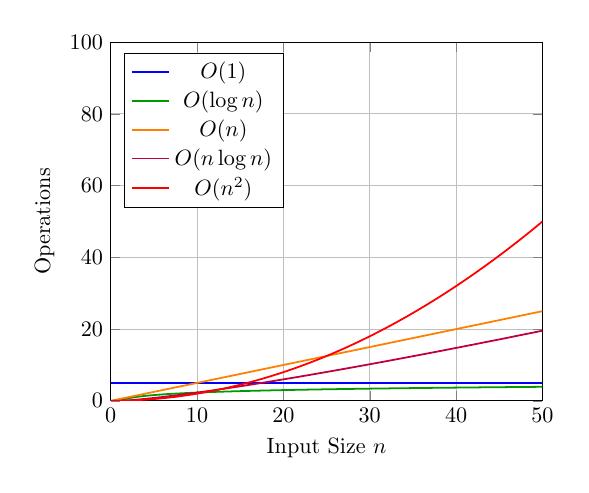
\begin{tikzpicture}[scale=0.8]
\begin{axis}[
    xlabel={Input Size $n$},
    ylabel={Operations},
    xmin=0, xmax=50,
    ymin=0, ymax=100,
    grid=major,
    legend pos=north west,
    samples=200
]

\addplot[blue, thick, domain=0:50] {5};
\addlegendentry{$O(1)$}

\addplot[green!60!black, thick, domain=1:50] {ln(x)};
\addlegendentry{$O(\log n)$}

\addplot[orange, thick, domain=0:50] {x/2};
\addlegendentry{$O(n)$}

\addplot[purple, thick, domain=1:50] {x*ln(x)/10};
\addlegendentry{$O(n\log n)$}

\addplot[red, thick, domain=0:50] {x^2/50};
\addlegendentry{$O(n^2)$}

\end{axis}
\end{tikzpicture}
\end{center}


\textbf{Growth Hierarchy (from best to worst):}
\[
O(1) \ll O(\log n) \ll O(n) \ll O(n \log n) \ll O(n^2) \ll O(2^n) \ll O(n!)
\]

\begin{keyidea}
For large $n$, the \textbf{shape of the curve} matters far more than constant factors. An $O(n)$ algorithm with a constant of 1000 will eventually beat an $O(n^2)$ algorithm with a constant of 1.
\end{keyidea}

\subsection{Concrete Examples: Time for $n = 1,000,000$}

Assuming 1 billion operations per second:

\begin{center}
\begin{tabular}{|c|c|c|}
\hline
\textbf{Complexity} & \textbf{Operations} & \textbf{Time} \\
\hline
$O(1)$ & 1 & 1 nanosecond \\
$O(\log n)$ & $\approx 20$ & 20 nanoseconds \\
$O(n)$ & $10^6$ & 1 millisecond \\
$O(n \log n)$ & $2 \times 10^7$ & 20 milliseconds \\
$O(n^2)$ & $10^{12}$ & \textbf{11.5 days} \\
$O(2^n)$ & $2^{1000000}$ & \textbf{Heat death of universe} \\
\hline
\end{tabular}
\end{center}

\section{Formal Definitions: The Mathematics of Big O}

\begin{definition}[Big O Notation]
We say $f(n) = O(g(n))$ if there exist constants $c > 0$ and $n_0 > 0$ such that:
\[
f(n) \leq c \cdot g(n) \quad \text{for all } n \geq n_0
\]
\end{definition}

\textbf{Translation:} $f$ grows no faster than $g$ (up to a constant multiple), for sufficiently large $n$.

\begin{example}
Prove that $3n^2 + 5n + 2 = O(n^2)$.

\textbf{Proof:} For $n \geq 1$:
\begin{align*}
3n^2 + 5n + 2 &\leq 3n^2 + 5n^2 + 2n^2 \\
&= 10n^2
\end{align*}
So choose $c = 10$ and $n_0 = 1$. Then $f(n) \leq 10 \cdot n^2$ for all $n \geq 1$.
\end{example}

\subsection{The Complete Family: Big O, Big Omega, Big Theta}

\begin{center}
\begin{tabular}{|c|l|l|}
\hline
\textbf{Notation} & \textbf{Meaning} & \textbf{Analogy} \\
\hline
$O(g(n))$ & Upper bound & "$\leq$" \\
$\Omega(g(n))$ & Lower bound & "$\geq$" \\
$\Theta(g(n))$ & Tight bound & "$=$" \\
\hline
\end{tabular}
\end{center}

\begin{definition}[Big Omega]
$f(n) = \Omega(g(n))$ if there exist $c > 0$ and $n_0 > 0$ such that:
\[
f(n) \geq c \cdot g(n) \quad \text{for all } n \geq n_0
\]
\end{definition}

\begin{definition}[Big Theta]
$f(n) = \Theta(g(n))$ if $f(n) = O(g(n))$ \textbf{and} $f(n) = \Omega(g(n))$.
\end{definition}

\begin{insight}
Big O is like saying "my algorithm takes \textit{at most} this long." Big Theta is saying "my algorithm takes \textit{exactly} this long (asymptotically)." Most of the time, we want Big Theta, but we often use Big O notation loosely to mean Theta.
\end{insight}

\section{Analyzing Code: From Python to Big O}

\subsection{Rule 1: Sequential Operations Add}

\begin{lstlisting}
def process_data(arr):
    # Step 1: O(n)
    total = sum(arr)
    
    # Step 2: O(n)
    for x in arr:
        print(x)
    
    # Step 3: O(1)
    return total / len(arr)
\end{lstlisting}

\textbf{Analysis:} $O(n) + O(n) + O(1) = O(n)$

\begin{keyidea}
When operations happen sequentially, we \textbf{add} their complexities, then take the dominant term.
\end{keyidea}

\subsection{Rule 2: Nested Loops Multiply}

\begin{lstlisting}
def print_pairs(arr):
    n = len(arr)
    for i in range(n):      # O(n)
        for j in range(n):  # O(n)
            print(arr[i], arr[j])
\end{lstlisting}

\textbf{Analysis:} Outer loop: $n$ iterations. Inner loop: $n$ iterations each.
Total: $n \times n = O(n^2)$

\subsection{Rule 3: Logarithmic Complexity from Halving}

\begin{lstlisting}
def binary_search(arr, target):
    left, right = 0, len(arr) - 1
    
    while left <= right:
        mid = (left + right) // 2
        if arr[mid] == target:
            return mid
        elif arr[mid] < target:
            left = mid + 1
        else:
            right = mid - 1
    
    return -1
\end{lstlisting}

\textbf{Analysis:} Each iteration cuts the search space in half.
\begin{align*}
n \to \frac{n}{2} \to \frac{n}{4} \to \cdots \to 1
\end{align*}

Number of halvings until we reach 1: $\log_2 n$

Therefore: $O(\log n)$

\begin{insight}
Whenever you see the input size being \textbf{divided} (usually by 2) at each step, think logarithmic complexity. This is the signature of divide-and-conquer algorithms.
\end{insight}

\section{The Master Method: A Preview}

For recursive algorithms of the form:
\[
T(n) = a \cdot T\left(\frac{n}{b}\right) + f(n)
\]

where we divide the problem into $a$ subproblems of size $\frac{n}{b}$, and $f(n)$ is the work to combine them.

\textbf{Quick Rules:}
\begin{enumerate}
    \item If $f(n) = O(n^c)$ where $c < \log_b a$, then $T(n) = \Theta(n^{\log_b a})$
    \item If $f(n) = \Theta(n^c \log^k n)$ where $c = \log_b a$, then $T(n) = \Theta(n^c \log^{k+1} n)$
    \item If $f(n) = \Omega(n^c)$ where $c > \log_b a$, then $T(n) = \Theta(f(n))$
\end{enumerate}

\textbf{We'll explore this deeply in later chapters.}

\section{Space Complexity: The Other Dimension}

Time isn't everything. Memory matters too!

\begin{lstlisting}
def create_matrix(n):
    # Creates an n x n matrix
    matrix = [[0] * n for _ in range(n)]
    return matrix
\end{lstlisting}

\textbf{Space Complexity:} $O(n^2)$ — we allocate $n \times n$ integers.

\subsection{Auxiliary Space vs Total Space}

\begin{itemize}
    \item \textbf{Total Space:} Input + auxiliary
    \item \textbf{Auxiliary Space:} Extra space used by algorithm (excluding input)
\end{itemize}

\begin{example}[In-place vs Not In-place]

\textbf{Not in-place} (creates new array):
\begin{lstlisting}
def reverse_copy(arr):
    return arr[::-1]  # O(n) auxiliary space
\end{lstlisting}

\textbf{In-place} (modifies original):
\begin{lstlisting}
def reverse_inplace(arr):
    left, right = 0, len(arr) - 1
    while left < right:
        arr[left], arr[right] = arr[right], arr[left]
        left += 1
        right -= 1
    # O(1) auxiliary space
\end{lstlisting}
\end{example}

\section{Best, Worst, and Average Case Analysis}

Not all inputs are created equal!

\begin{example}[Linear Search]
\begin{lstlisting}
def linear_search(arr, target):
    for i in range(len(arr)):
        if arr[i] == target:
            return i
    return -1
\end{lstlisting}

\textbf{Best Case:} $O(1)$ — target is first element \\
\textbf{Worst Case:} $O(n)$ — target is last or not present \\
\textbf{Average Case:} $O(n/2) = O(n)$ — target equally likely anywhere
\end{example}

\begin{keyidea}
We typically analyze \textbf{worst-case} complexity because it gives guarantees. Average-case requires assumptions about input distribution.
\end{keyidea}

\section{Common Complexity Classes: A Visual Guide}

\begin{center}
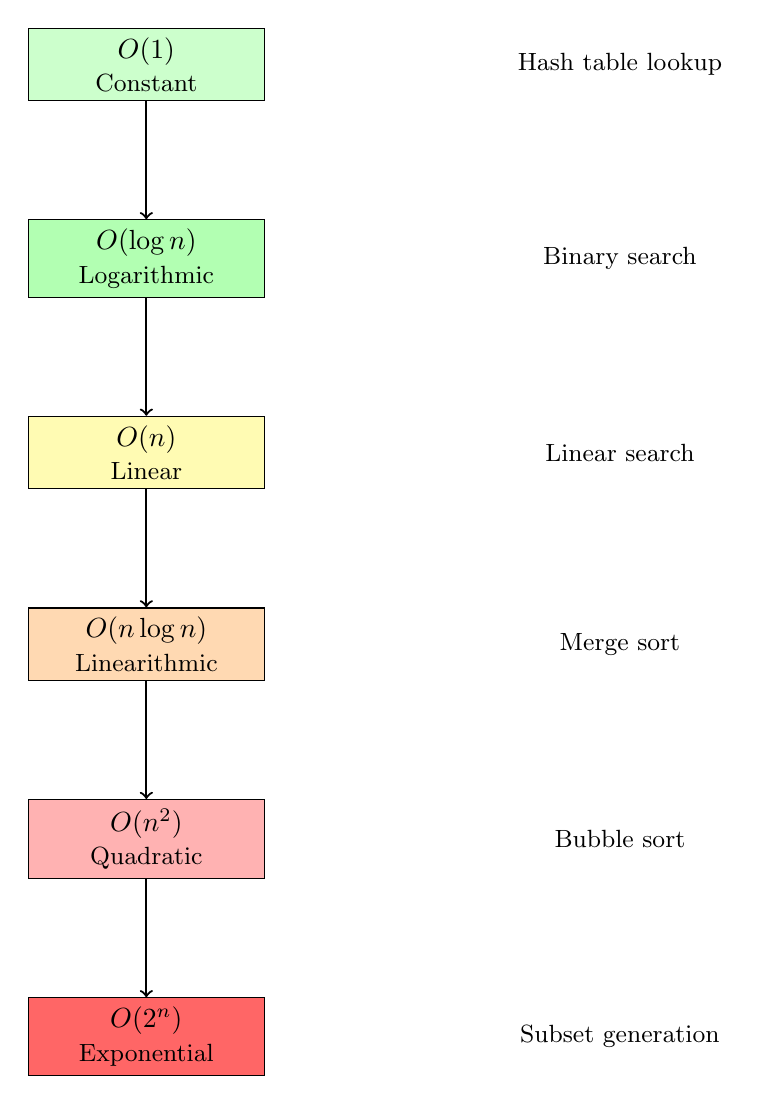
\begin{tikzpicture}[
    node distance=1.5cm,
    every node/.style={rectangle, draw, minimum width=3cm, minimum height=0.8cm, align=center}
]
    \node (constant) [fill=green!20] {$O(1)$ \\ \small Constant};
    \node (log) [below=of constant, fill=green!30] {$O(\log n)$ \\ \small Logarithmic};
    \node (linear) [below=of log, fill=yellow!30] {$O(n)$ \\ \small Linear};
    \node (nlogn) [below=of linear, fill=orange!30] {$O(n \log n)$ \\ \small Linearithmic};
    \node (quadratic) [below=of nlogn, fill=red!30] {$O(n^2)$ \\ \small Quadratic};
    \node (exponential) [below=of quadratic, fill=red!60] {$O(2^n)$ \\ \small Exponential};
    
    \draw[->, thick] (constant) -- (log);
    \draw[->, thick] (log) -- (linear);
    \draw[->, thick] (linear) -- (nlogn);
    \draw[->, thick] (nlogn) -- (quadratic);
    \draw[->, thick] (quadratic) -- (exponential);
    
    \node[right=3cm of constant, draw=none] {\small Hash table lookup};
    \node[right=3cm of log, draw=none] {\small Binary search};
    \node[right=3cm of linear, draw=none] {\small Linear search};
    \node[right=3cm of nlogn, draw=none] {\small Merge sort};
    \node[right=3cm of quadratic, draw=none] {\small Bubble sort};
    \node[right=3cm of exponential, draw=none] {\small Subset generation};
\end{tikzpicture}
\end{center}

\section{Practice Problems}

\subsection{Problem 1: Analyze This Code}

\begin{lstlisting}
def mystery_function(n):
    count = 0
    i = n
    while i > 0:
        j = 0
        while j < n:
            count += 1
            j += 1
        i = i // 2
    return count
\end{lstlisting}

\textbf{Solution:} 
\begin{itemize}
    \item Outer loop: $i$ is halved each time, so $\log n$ iterations
    \item Inner loop: Always runs $n$ times
    \item Total: $O(n \log n)$
\end{itemize}

\subsection{Problem 2: True or False?}

\begin{enumerate}
    \item $n^2 + 100n = O(n^2)$ \hfill \textbf{TRUE}
    \item $2^n = O(n^2)$ \hfill \textbf{FALSE}
    \item $\log(n^2) = O(\log n)$ \hfill \textbf{TRUE} (since $\log(n^2) = 2\log n$)
    \item $n! = O(2^n)$ \hfill \textbf{FALSE} ($n!$ grows faster)
\end{enumerate}

\subsection{Problem 3: Space vs Time Tradeoff}

\begin{lstlisting}
# Version 1: Time O(n), Space O(1)
def has_duplicates_v1(arr):
    n = len(arr)
    for i in range(n):
        for j in range(i+1, n):
            if arr[i] == arr[j]:
                return True
    return False

# Version 2: Time O(n), Space O(n)
def has_duplicates_v2(arr):
    seen = set()
    for x in arr:
        if x in seen:
            return True
        seen.add(x)
    return False
\end{lstlisting}

\textbf{Question:} Which is better?

\textbf{Answer:} Depends on constraints! If memory is tight, use v1. If speed matters and memory is available, use v2. This is the essence of algorithm design.

\section{Key Takeaways}

\begin{enumerate}
    \item \textbf{Big O describes growth rate}, not exact running time
    \item \textbf{Drop constants and lower-order terms}: $3n^2 + 5n = O(n^2)$
    \item \textbf{Sequential = Add, Nested = Multiply}
    \item \textbf{Halving = Logarithmic}
    \item \textbf{Consider both time and space complexity}
    \item \textbf{Worst-case analysis gives guarantees}
\end{enumerate}

\begin{insight}
Gilbert Strang often says: "Mathematics is not about formulas, it's about understanding." The same is true for algorithms. Big O notation is not about memorizing formulas—it's about developing an intuition for how algorithms scale. Once you have that intuition, the notation becomes second nature.
\end{insight}

\section{Looking Ahead}

In Chapter 2, we'll apply these concepts to our first data structure: \textbf{Arrays and Lists}. We'll see how different operations (access, insertion, deletion) have different complexities, and why understanding these tradeoffs is crucial for choosing the right data structure.

\vspace{1cm}

\begin{center}
\rule{0.5\textwidth}{0.4pt}

\textit{"An algorithm must be seen to be believed."} — Donald Knuth

\rule{0.5\textwidth}{0.4pt}
\end{center}
\pagebreak

\section{Chapter 2: Arrays, Lists, and Dynamic Arrays}
\subsection*{The Foundation of All Data Structures}

\begin{center}
\textit{"To understand a data structure, imagine you're the computer's memory manager."} — Our Journey Begins
\end{center}

\section{The Big Picture: What Problem Are We Solving?}

Imagine you're organizing a music playlist with 1000 songs. You need to:
\begin{enumerate}
    \item Play song number 437 instantly
    \item Add a new song at the end
    \item Insert a song in the middle of your favorites
    \item Remove a song you don't like anymore
\end{enumerate}

Different data structures make different operations fast or slow. Let's start from absolute zero and build up!

\begin{insight}
The most fundamental question in computer science: \textbf{"Where do we put stuff in memory, and how do we find it again?"} Everything else builds on this.
\end{insight}

\section{First Principles: How Computer Memory Actually Works}

\subsection{Memory is Like an Apartment Building}

Think of your computer's memory (RAM) as a giant apartment building with billions of rooms. Each room:
\begin{itemize}
    \item Has a unique \textbf{address} (like "Room 1043")
    \item Can store one piece of data (a number, a letter, etc.)
    \item Is the same size as every other room
\end{itemize}

\begin{center}
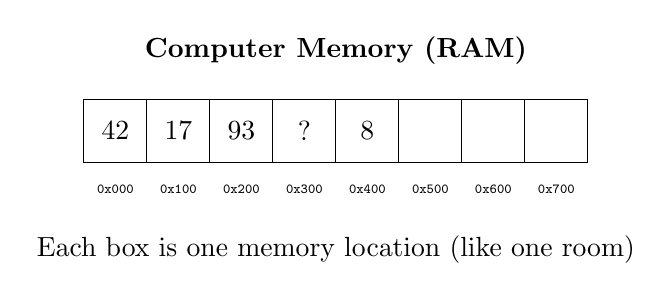
\begin{tikzpicture}[scale=0.8]
    % Draw memory cells
    \foreach \x in {0,1,2,3,4,5,6,7} {
        \draw (\x,0) rectangle (\x+1,1);
        \node[below] at (\x+0.5, -0.2) {\tiny \texttt{0x\x 00}};
    }
    
    % Add some data
    \node at (0.5, 0.5) {42};
    \node at (1.5, 0.5) {17};
    \node at (2.5, 0.5) {93};
    \node at (3.5, 0.5) {?};
    \node at (4.5, 0.5) {8};
    
    \node[above] at (4, 1.4) {\textbf{Computer Memory (RAM)}};
    \node[below] at (4, -1) {Each box is one memory location (like one room)};
\end{tikzpicture}
\end{center}

\textbf{Key Fact:} If you know the address, you can jump to that room \textbf{instantly} — this is called \textbf{random access}. It takes the same time whether it's room 5 or room 5 million!

\section{The Array: Sequential Rooms in a Row}

\subsection{Mental Model: A Row of Lockers}

An array is like renting a \textbf{row of consecutive rooms} in our memory building.

\begin{center}
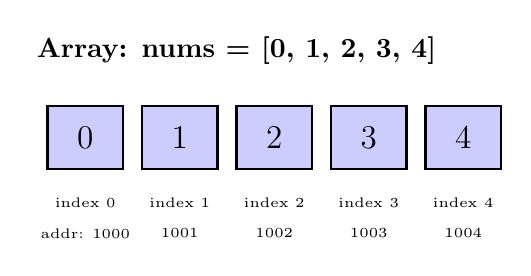
\begin{tikzpicture}[scale=0.8]
    % Array visualization
    \foreach \x in {0,1,2,3,4} {
        \draw[thick, fill=blue!20] (\x*1.5,0) rectangle (\x*1.5+1.2,1);
        \node at (\x*1.5+0.6, 0.5) {\large \x};
    }
    
    % Labels
    \node[above] at (3, 1.5) {\textbf{Array: nums = [0, 1, 2, 3, 4]}};
    
    % Index labels
    \foreach \x in {0,1,2,3,4} {
        \node[below] at (\x*1.5+0.6, -0.3) {\tiny index \x};
    }
    
    % Memory addresses
    \node[below] at (0.6, -0.8) {\tiny addr: 1000};
    \node[below] at (2.1, -0.8) {\tiny 1001};
    \node[below] at (3.6, -0.8) {\tiny 1002};
    \node[below] at (5.1, -0.8) {\tiny 1003};
    \node[below] at (6.6, -0.8) {\tiny 1004};
\end{tikzpicture}
\end{center}

\begin{keyidea}
\textbf{The Magic Formula:} If the array starts at address 1000, where is element at index 3?

\[
\text{Address of element[i]} = \text{start\_address} + (\text{i} \times \text{element\_size})
\]

So element[3] is at: $1000 + (3 \times 1) = 1003$

This is why accessing \texttt{nums[437]} is just as fast as \texttt{nums[0]} — it's just one calculation!
\end{keyidea}

\subsection{Python Lists ARE Arrays (Mostly)}

In Python, when you write:
\begin{lstlisting}
nums = [10, 20, 30, 40, 50]
\end{lstlisting}

Python creates an array behind the scenes. Let's see what we can do:

\begin{lstlisting}
# Access - O(1) - INSTANT!
print(nums[2])  # Prints 30

# Update - O(1) - INSTANT!
nums[2] = 999   # Now nums = [10, 20, 999, 40, 50]

# Length - O(1) - INSTANT!
print(len(nums))  # Prints 5
\end{lstlisting}

\textbf{Why so fast?} The computer just jumps to the exact memory address. No searching needed!

\section{The Problem: Arrays Have Fixed Size}

\subsection{What Happens When We Run Out of Space?}

Here's the harsh reality: when you create an array of size 5, you get exactly 5 consecutive rooms. What if you want to add a 6th element?

\begin{center}
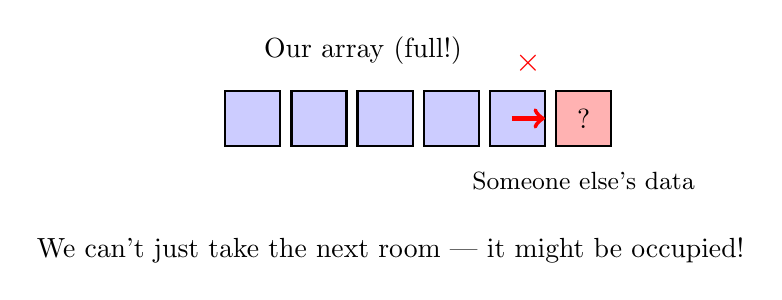
\begin{tikzpicture}[scale=0.7]
    % Original array
    \foreach \x in {0,1,2,3,4} {
        \draw[thick, fill=blue!20] (\x*1.2,2) rectangle (\x*1.2+1,3);
    }
    \node[above] at (2.5, 3.3) {Our array (full!)};
    
    % Someone else's data
    \draw[thick, fill=red!30] (6,2) rectangle (7,3);
    \node at (6.5, 2.5) {?};
    \node[below] at (6.5, 1.7) {\small Someone else's data};
    
    % Can't expand
    \draw[->, ultra thick, red] (5.2, 2.5) -- (5.8, 2.5);
    \node[red] at (5.5, 3.5) {\large $\times$};
    
    \node[below] at (3, 0.5) {We can't just take the next room — it might be occupied!};
\end{tikzpicture}
\end{center}

\textbf{Solution:} We have to:
\begin{enumerate}
    \item Find a new, bigger space (say, 10 rooms)
    \item Copy all our data to the new space
    \item Free up the old space
\end{enumerate}

This is \textbf{expensive}! But Python does this automatically for you.

\section{Dynamic Arrays: The Clever Trick}

\subsection{The Doubling Strategy}

Python lists are \textbf{dynamic arrays}. Here's the genius idea:

\begin{keyidea}
When the array gets full:
\begin{enumerate}
    \item Create a new array that's \textbf{twice as big}
    \item Copy everything over
    \item Add your new element
\end{enumerate}

Why double? Because it means we don't have to resize very often!
\end{keyidea}

\begin{center}
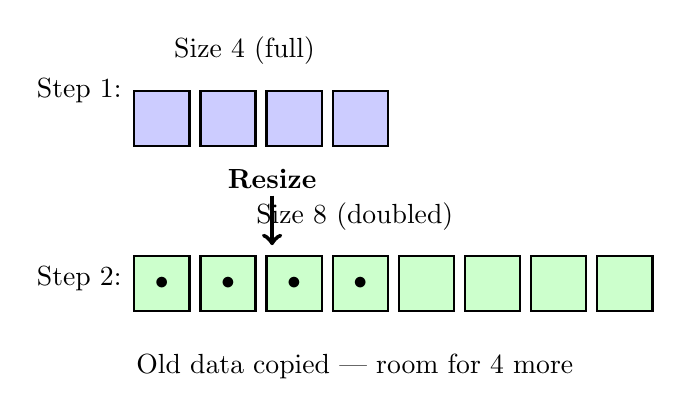
\begin{tikzpicture}[scale=0.7]

    % ---------------- Step 1 ----------------
    \node at (-1, 5) {Step 1:};
    \foreach \x in {0,1,2,3} {
        \draw[thick, fill=blue!20] (\x*1.2,4) rectangle (\x*1.2+1,5);
    }
    \node[above] at (2, 5.3) {Size 4 (full)};
    
    % ---------------- Arrow ----------------
    \node at (2.5, 3.4) {\textbf{Resize}};
    \draw[->, ultra thick] (2.5, 3.1) -- (2.5, 2.2);
    
    % ---------------- Step 2 ----------------
    \node at (-1, 1.6) {Step 2:};
    \foreach \x in {0,1,2,3,4,5,6,7} {
        \draw[thick, fill=green!20] (\x*1.2,1) rectangle (\x*1.2+1,2);
    }
    \node[above] at (4, 2.3) {Size 8 (doubled)};
    
    % ---------------- Copied data ----------------
    \foreach \x in {0,1,2,3} {
        \node at (\x*1.2+0.5, 1.5) {$\bullet$};
    }
    \node[below] at (4, 0.4) {Old data copied — room for 4 more};

\end{tikzpicture}
\end{center}

\subsection{Amortized Analysis: The Sneaky Math}

Let's add 8 elements to an empty dynamic array starting with size 1:

\begin{center}
\begin{tabular}{|c|c|c|c|}
\hline
\textbf{Element \#} & \textbf{Array Size} & \textbf{Resize?} & \textbf{Copies Made} \\
\hline
1 & 1 & Yes (size 1) & 0 \\
2 & 2 & Yes (size 2) & 1 \\
3 & 4 & Yes (size 4) & 2 \\
4 & 4 & No & 0 \\
5 & 8 & Yes (size 8) & 4 \\
6 & 8 & No & 0 \\
7 & 8 & No & 0 \\
8 & 8 & No & 0 \\
\hline
\multicolumn{3}{|r|}{\textbf{Total copies:}} & \textbf{7} \\
\hline
\end{tabular}
\end{center}

Total work: 8 insertions + 7 copies = 15 operations for 8 elements.

Average per insertion: $15/8 \approx 1.875$ operations

\begin{insight}
Even though \textit{some} insertions are expensive (when we resize), \textit{most} are cheap. On average, appending is $O(1)$ — we call this \textbf{amortized $O(1)$}.

Think of it like paying rent: most months you just pay rent (cheap), but occasionally you also pay a security deposit (expensive). On average over many months, the cost per month is still low.
\end{insight}

\section{Array Operations: The Complete Picture}

\begin{center}
\begin{tabular}{|l|c|l|}
\hline
\textbf{Operation} & \textbf{Time} & \textbf{Why?} \\
\hline
\texttt{arr[i]} (access) & $O(1)$ & Jump to address directly \\
\texttt{arr[i] = x} (update) & $O(1)$ & Jump to address, write \\
\texttt{len(arr)} & $O(1)$ & Stored as metadata \\
\texttt{arr.append(x)} & $O(1)^*$ & Amortized (usually free space) \\
\texttt{arr.pop()} & $O(1)$ & Remove from end \\
\texttt{arr.insert(i, x)} & $O(n)$ & Need to shift elements \\
\texttt{arr.remove(x)} & $O(n)$ & Search + shift \\
\texttt{arr.pop(i)} & $O(n)$ & Need to shift elements \\
\hline
\end{tabular}

*Amortized constant time
\end{center}

\subsection{Why is Insert in the Middle So Slow?}
\begin{center}
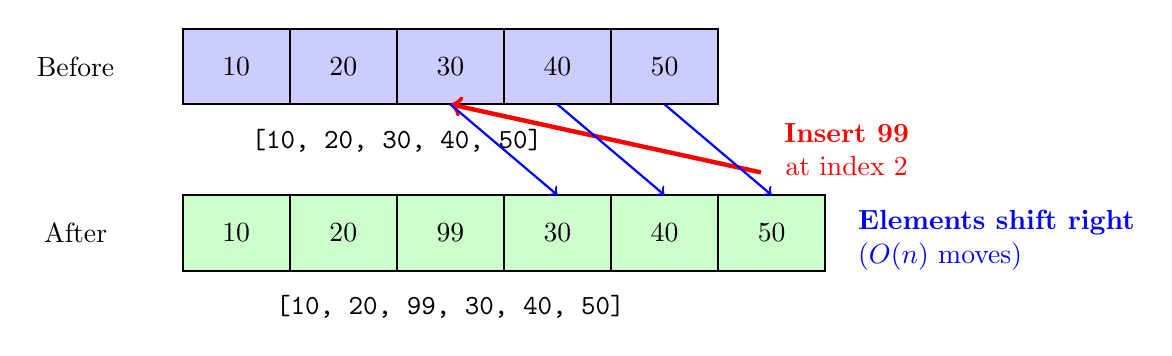
\begin{tikzpicture}[scale=0.8, x=1.7cm, y=1.2cm]

    % ---------------- Before ----------------
    \node at (-1, 3) {Before};
    \foreach \x/\val in {0/10,1/20,2/30,3/40,4/50} {
        \draw[thick, fill=blue!20] (\x,2.5) rectangle (\x+1,3.5);
        \node at (\x+0.5,3) {\val};
    }
    \node[below] at (2,2.3) {\texttt{[10, 20, 30, 40, 50]}};

    % ---------------- Insert annotation ----------------
    \node[red, align=center] at (6.2,1.9)
        {\textbf{Insert 99}\\at index 2};
    \draw[->, ultra thick, red] (5.4,1.6) -- (2.5,2.5);

    % ---------------- After ----------------
    \node at (-1,0.8) {After};
    \foreach \x/\val in {0/10,1/20,2/99,3/30,4/40,5/50} {
        \draw[thick, fill=green!20] (\x,0.3) rectangle (\x+1,1.3);
        \node at (\x+0.5,0.8) {\val};
    }
    \node[below] at (2.5,0.1) {\texttt{[10, 20, 99, 30, 40, 50]}};

    % ---------------- Shift arrows ----------------
    \draw[->, thick, blue] (2.5,2.5) -- (3.5,1.3);
    \draw[->, thick, blue] (3.5,2.5) -- (4.5,1.3);
    \draw[->, thick, blue] (4.5,2.5) -- (5.5,1.3);

    % ---------------- Shift label (safe zone) ----------------
    \node[blue, align=left] at (7.6,0.7)
        {\textbf{Elements shift right}\\($O(n)$ moves)};

\end{tikzpicture}
\end{center}

\textbf{The Work Required:}
\begin{enumerate}
    \item Make space by shifting all elements after index 2 to the right
    \item In worst case (insert at index 0), shift $n$ elements
    \item Therefore: $O(n)$ time
\end{enumerate}

\section{Python List Examples: Learning by Doing}

\subsection{Example 1: Building Your Intuition}

\begin{lstlisting}
# Create a list
numbers = [5, 2, 8, 1, 9]

# Fast operations - O(1)
print(numbers[2])        # 8 - instant access
numbers[2] = 100         # instant update
numbers.append(7)        # add at end (amortized O(1))
numbers.pop()            # remove from end - O(1)

# Slow operations - O(n)
numbers.insert(0, 999)   # insert at start - shifts everyone!
numbers.remove(2)        # find and remove - must search
first = numbers.pop(0)   # remove from start - shifts everyone!
\end{lstlisting}

\subsection{Example 2: When Does the Resizing Happen?}

\begin{lstlisting}
import sys

arr = []
previous_size = 0

for i in range(20):
    arr.append(i)
    current_size = sys.getsizeof(arr)
    
    if current_size != previous_size:
        print(f"After adding element {i}:")
        print(f"  Array capacity changed to ~{len(arr)} elements")
        previous_size = current_size
\end{lstlisting}

\textbf{Output (approximate):}
\begin{verbatim}
After adding element 0: Array capacity changed
After adding element 4: Array capacity changed  
After adding element 8: Array capacity changed
After adding element 16: Array capacity changed
\end{verbatim}

See the doubling pattern? Python grows the array strategically!

\section{Common Patterns and Tricks}

\subsection{Pattern 1: Two Pointers}

When you need to work with two positions in an array:

\begin{lstlisting}
def reverse_array(arr):
    """Reverse array in-place using two pointers"""
    left = 0
    right = len(arr) - 1
    
    while left < right:
        # Swap elements
        arr[left], arr[right] = arr[right], arr[left]
        left += 1
        right -= 1
    
    return arr

# Example
nums = [1, 2, 3, 4, 5]
reverse_array(nums)  # nums is now [5, 4, 3, 2, 1]
\end{lstlisting}

\textbf{Time:} $O(n)$ — visit each element once \\
\textbf{Space:} $O(1)$ — only use two variables!

\subsection{Pattern 2: Sliding Window}

Find the sum of every 3 consecutive elements:

\begin{lstlisting}
def sliding_window_sum(arr, k=3):
    """Find max sum of k consecutive elements"""
    if len(arr) < k:
        return None
    
    # Compute first window
    window_sum = sum(arr[0:k])
    max_sum = window_sum
    
    # Slide the window
    for i in range(k, len(arr)):
        # Remove leftmost element, add rightmost element
        window_sum = window_sum - arr[i-k] + arr[i]
        max_sum = max(max_sum, window_sum)
    
    return max_sum

# Example: find max sum of 3 consecutive numbers
nums = [1, 3, 2, 6, -1, 4, 1, 8, 2]
print(sliding_window_sum(nums, 3))  # 13 (from 4+1+8)
\end{lstlisting}

\textbf{Time:} $O(n)$ — one pass through array \\
\textbf{Space:} $O(1)$ — only store the sum

\section{Lists vs Arrays in Other Languages}

\begin{center}
\begin{tabular}{|l|l|l|}
\hline
\textbf{Language} & \textbf{Fixed Array} & \textbf{Dynamic Array} \\
\hline
Python & (Use NumPy) & \texttt{list} \\
Java & \texttt{int[]} & \texttt{ArrayList} \\
C++ & \texttt{int arr[]} & \texttt{vector} \\
JavaScript & — & \texttt{Array} \\
\hline
\end{tabular}
\end{center}

\section{Practice Problems}

\subsection{Problem 1: Remove Duplicates (In-Place)}

Given a sorted array, remove duplicates without using extra space.

\begin{lstlisting}
def remove_duplicates(arr):
    """
    Remove duplicates from sorted array in-place.
    Return the new length.
    """
    if not arr:
        return 0
    
    # Write pointer - where to place next unique element
    write_idx = 1
    
    # Read through array
    for read_idx in range(1, len(arr)):
        # If different from previous, it's unique
        if arr[read_idx] != arr[read_idx - 1]:
            arr[write_idx] = arr[read_idx]
            write_idx += 1
    
    return write_idx

# Test
nums = [1, 1, 2, 2, 2, 3, 4, 4, 5]
new_length = remove_duplicates(nums)
print(nums[:new_length])  # [1, 2, 3, 4, 5]
\end{lstlisting}

\textbf{Analysis:}
\begin{itemize}
    \item Time: $O(n)$ — single pass
    \item Space: $O(1)$ — no extra arrays
    \item Key idea: Two pointers (read and write)
\end{itemize}

\subsection{Problem 2: Rotate Array}

Rotate array to the right by $k$ positions.

\begin{lstlisting}
def rotate_array(arr, k):
    """
    Rotate array to the right by k positions.
    Example: [1,2,3,4,5], k=2 -> [4,5,1,2,3]
    """
    n = len(arr)
    k = k % n  # Handle k > n
    
    # Helper function to reverse portion of array
    def reverse(start, end):
        while start < end:
            arr[start], arr[end] = arr[end], arr[start]
            start += 1
            end -= 1
    
    # Three reverses trick!
    reverse(0, n - 1)      # Reverse entire array
    reverse(0, k - 1)      # Reverse first k elements
    reverse(k, n - 1)      # Reverse remaining elements
    
    return arr

# Test
nums = [1, 2, 3, 4, 5]
rotate_array(nums, 2)
print(nums)  # [4, 5, 1, 2, 3]
\end{lstlisting}

\begin{keyidea}
\textbf{The Reversal Trick:}
\begin{align*}
[1,2,3,4,5] &\xrightarrow{\text{reverse all}} [5,4,3,2,1] \\
&\xrightarrow{\text{reverse first 2}} [4,5,3,2,1] \\
&\xrightarrow{\text{reverse last 3}} [4,5,1,2,3]
\end{align*}

This is a classic example of clever thinking making algorithms elegant!
\end{keyidea}

\subsection{Problem 3: Find Missing Number}

Array contains $n$ distinct numbers from $0$ to $n$. One is missing. Find it.

\begin{lstlisting}
def find_missing(arr):
    """
    Array has numbers 0 to n with one missing.
    Example: [0,1,3] -> missing is 2
    """
    n = len(arr)
    
    # Expected sum: 0+1+2+...+n = n*(n+1)/2
    expected_sum = n * (n + 1) // 2
    
    # Actual sum
    actual_sum = sum(arr)
    
    # Difference is the missing number
    return expected_sum - actual_sum

# Test
print(find_missing([0, 1, 3]))  # 2
print(find_missing([0, 1, 2, 3, 4, 6]))  # 5
\end{lstlisting}

\textbf{Analysis:}
\begin{itemize}
    \item Time: $O(n)$
    \item Space: $O(1)$
    \item Key idea: Mathematical formula instead of searching!
\end{itemize}

\section{Memory Layout: Seeing Like the Computer}

Let's visualize what actually happens in memory:

\begin{lstlisting}
# In Python
my_list = [10, 20, 30]
\end{lstlisting}

\begin{center}
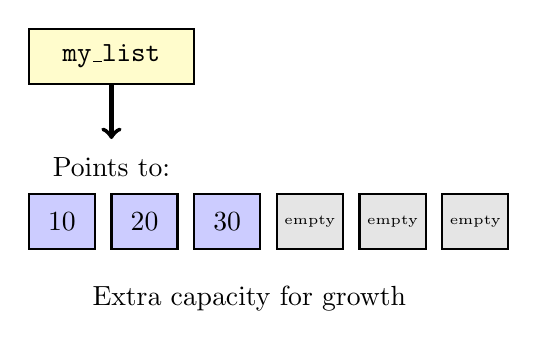
\begin{tikzpicture}[scale=0.7]
    % The list object
    \draw[thick, fill=yellow!20] (0,3) rectangle (3,4);
    \node at (1.5, 3.5) {\texttt{my\_list}};
    
    % Arrow to array
    \draw[->, ultra thick] (1.5, 3) -- (1.5, 2);
    
    % The actual array in memory
    \node at (1.5, 1.5) {Points to:};
    \foreach \x/\val in {0/10,1/20,2/30} {
        \draw[thick, fill=blue!20] (\x*1.5,0) rectangle (\x*1.5+1.2,1);
        \node at (\x*1.5+0.6, 0.5) {\val};
    }
    
    % Extra capacity (not visible to user)
    \foreach \x in {3,4,5} {
        \draw[thick, fill=gray!20] (\x*1.5,0) rectangle (\x*1.5+1.2,1);
        \node at (\x*1.5+0.6, 0.5) {\tiny empty};
    }
    
    \node[below] at (4, -0.5) {Extra capacity for growth};
\end{tikzpicture}
\end{center}

\section{Key Takeaways: What You Must Remember}

\begin{enumerate}
    \item \textbf{Arrays are contiguous memory} — elements sit next to each other like a row of lockers
    
    \item \textbf{Random access is magic} — accessing \texttt{arr[i]} is $O(1)$ because:
    \[
    \text{address} = \text{start} + (i \times \text{element\_size})
    \]
    
    \item \textbf{Dynamic arrays double in size} — this makes append $O(1)$ amortized
    
    \item \textbf{Inserting in middle is expensive} — requires shifting $n$ elements, so $O(n)$
    
    \item \textbf{Think about tradeoffs}:
    \begin{itemize}
        \item Good at: Random access, appending
        \item Bad at: Inserting/deleting in middle, resizing
    \end{itemize}
\end{enumerate}

\begin{insight}
Gilbert Strang would say: "Don't just memorize the complexities. Understand \textit{why} they are what they are. Picture the memory, imagine the shifting, feel the doubling. Once you truly see it, you'll never forget it."
\end{insight}

\section{Looking Ahead to Chapter 3}

Arrays are fast for access but slow for insertion. What if we need fast insertion?

That's where \textbf{Linked Lists} come in — a completely different way of organizing data where elements can live anywhere in memory, connected by pointers like a treasure hunt!

But that's for next time...

\vspace{1cm}

\begin{center}
\rule{0.5\textwidth}{0.4pt}

\textit{"The secret to understanding algorithms is to think like the computer, but explain like a teacher."}

\rule{0.5\textwidth}{0.4pt}
\end{center}
\pagebreak
\section{Chapter 3: Recursion and the Call Stack}
\subsection*{How Functions Call Themselves (And Why Your Brain Will Hurt, Then Click)}

\begin{center}
\textit{"To understand recursion, you must first understand recursion."} — Classic Programmer Joke
\end{center}

\section{The Big Picture: What IS Recursion?}

Imagine you're in a line of 100 people waiting for concert tickets. You want to know your position. You could:

\textbf{Option 1 (Iterative):} Walk to the front, count everyone, walk back. \\
\textbf{Option 2 (Recursive):} Ask the person in front of you: "What's your position?" Then add 1.

The person in front asks the person in front of them, and so on, until someone at the front says "I'm first!" Then the answer travels back.

\begin{keyidea}
\textbf{Recursion} is when a function calls itself to solve a smaller version of the same problem.

It's like those Russian nesting dolls — each doll contains a smaller version of itself, until you reach the tiniest one.
\end{keyidea}

\begin{center}
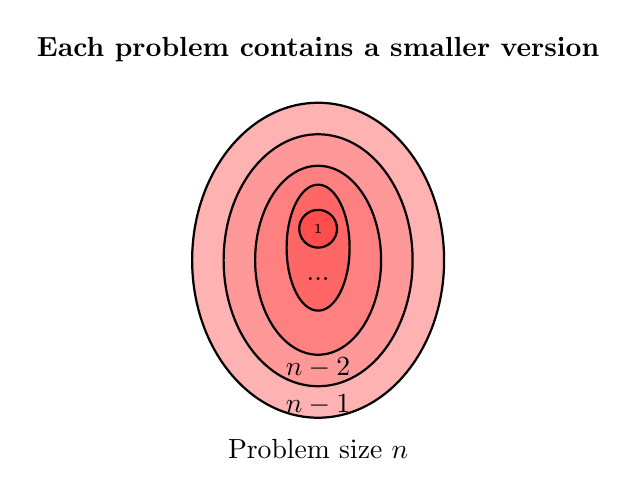
\begin{tikzpicture}[scale=0.8]
    % Matryoshka dolls representation
    \draw[thick, fill=red!30] (0,0) ellipse (2 and 2.5);
    \node at (0, -3) {Problem size $n$};
    
    \draw[thick, fill=red!40] (0,0) ellipse (1.5 and 2);
    \node at (0, -2.3) {$n-1$};
    
    \draw[thick, fill=red!50] (0,0) ellipse (1 and 1.5);
    \node at (0, -1.7) {$n-2$};
    
    \draw[thick, fill=red!60] (0,0.2) ellipse (0.5 and 1);
    \node at (0, -0.3) {$...$};
    
    \draw[thick, fill=red!70] (0,0.5) circle (0.3);
    \node at (0, 0.5) {\tiny 1};
    
    \node[above] at (0, 3) {\textbf{Each problem contains a smaller version}};
\end{tikzpicture}
\end{center}

\section{First Principles: How Do Functions Actually Work?}

\subsection{The Call Stack: Your Computer's To-Do List}

When you call a function, the computer needs to remember:
\begin{enumerate}
    \item Where to return when the function finishes
    \item The function's local variables
    \item The function's parameters
\end{enumerate}

This information is stored in a \textbf{stack} — think of it like a stack of plates.

\begin{center}
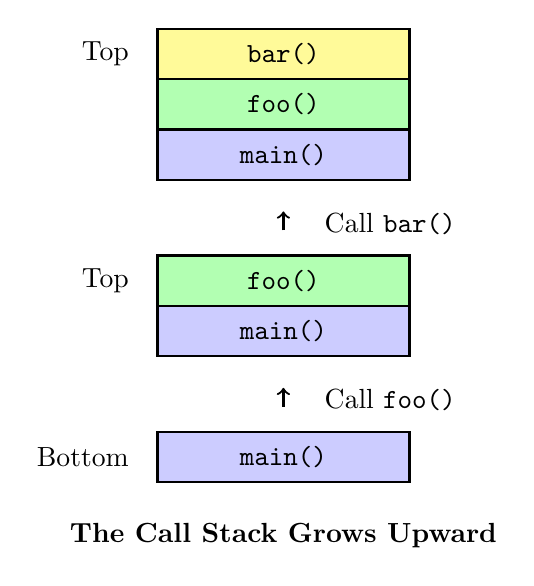
\begin{tikzpicture}[scale=0.8]
    % Stack visualization
    \draw[thick, fill=blue!20] (0,0) rectangle (4,0.8);
    \node at (2, 0.4) {\texttt{main()}};
    \node[left] at (-0.3, 0.4) {Bottom};
    
    \draw[->, thick] (2, 1.2) -- (2, 1.5);
    \node[right] at (2.5, 1.3) {Call \texttt{foo()}};
    
    \draw[thick, fill=blue!20] (0,2) rectangle (4,2.8);
    \node at (2, 2.4) {\texttt{main()}};
    \draw[thick, fill=green!30] (0,2.8) rectangle (4,3.6);
    \node at (2, 3.2) {\texttt{foo()}};
    \node[left] at (-0.3, 3.2) {Top};
    
    \draw[->, thick] (2, 4) -- (2, 4.3);
    \node[right] at (2.5, 4.1) {Call \texttt{bar()}};
    
    \draw[thick, fill=blue!20] (0,4.8) rectangle (4,5.6);
    \node at (2, 5.2) {\texttt{main()}};
    \draw[thick, fill=green!30] (0,5.6) rectangle (4,6.4);
    \node at (2, 6.0) {\texttt{foo()}};
    \draw[thick, fill=yellow!40] (0,6.4) rectangle (4,7.2);
    \node at (2, 6.8) {\texttt{bar()}};
    \node[left] at (-0.3, 6.8) {Top};
    
    \node[below] at (2, -0.5) {\textbf{The Call Stack Grows Upward}};
\end{tikzpicture}
\end{center}

\textbf{Key Rules:}
\begin{itemize}
    \item \textbf{Push:} When you call a function, add it to the top
    \item \textbf{Pop:} When a function returns, remove it from the top
    \item \textbf{LIFO:} Last In, First Out (like a stack of plates!)
\end{itemize}

\section{Your First Recursive Function: Countdown}

Let's write the simplest recursive function:

\begin{lstlisting}
def countdown(n):
    # Base case: when to stop
    if n == 0:
        print("Blastoff!")
        return
    
    # Recursive case: do work and call yourself
    print(n)
    countdown(n - 1)  # Call with smaller problem

# Try it!
countdown(3)
\end{lstlisting}

\textbf{Output:}
\begin{verbatim}
3
2
1
Blastoff!
\end{verbatim}

\subsection{What Happens in Memory (Step by Step)}

\begin{center}
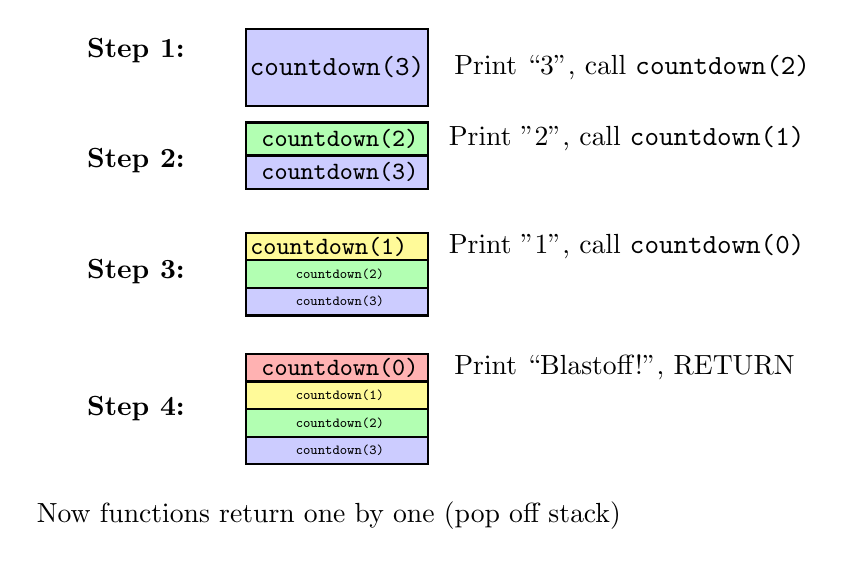
\begin{tikzpicture}[scale=0.7]
    % Step 1
    \node at (-2, 6) {\textbf{Step 1:}};

    \draw[thick, fill=blue!20] (0,5.0) rectangle (3.3,6.4);
    \node at (1.65, 5.7) {\texttt{countdown(3)}};

    \node[right] at (3.6, 5.7)
        {Print ``3'', call \texttt{countdown(2)}};
    
    % Step 2
    \node at (-2, 4) {\textbf{Step 2:}};
    \draw[thick, fill=blue!20] (0,3.5) rectangle (3.3,4.1);
    \node[font=\small] at (1.7, 3.8) {\texttt{countdown(3)}};
    \draw[thick, fill=green!30] (0,4.1) rectangle (3.3,4.7);
    \node[font=\small] at (1.7, 4.4) {\texttt{countdown(2)}};
    \node[right] at (3.5, 4.4) {Print "2", call \texttt{countdown(1)}};
    
    % Step 3
    \node at (-2, 2) {\textbf{Step 3:}};
    \draw[thick, fill=blue!20] (0,1.2) rectangle (3.3,1.7);
    \node[font=\tiny] at (1.7, 1.45) {\texttt{countdown(3)}};
    \draw[thick, fill=green!30] (0,1.7) rectangle (3.3,2.2);
    \node[font=\tiny] at (1.7, 1.95) {\texttt{countdown(2)}};
    \draw[thick, fill=yellow!40] (0,2.2) rectangle (3.3,2.7);
    \node[font=\small] at (1.5, 2.45) {\texttt{countdown(1)}};
    \node[right] at (3.5, 2.45) {Print "1", call \texttt{countdown(0)}};
    
    % Step 4
    \node at (-2, -0.5) {\textbf{Step 4:}};

    \draw[thick, fill=blue!20] (0,-1.5) rectangle (3.3,-1.0);
    \node[font=\tiny] at (1.7, -1.25) {\texttt{countdown(3)}};

    \draw[thick, fill=green!30] (0,-1.0) rectangle (3.3,-0.5);
    \node[font=\tiny] at (1.7, -0.75) {\texttt{countdown(2)}};

    \draw[thick, fill=yellow!40] (0,-0.5) rectangle (3.3,0);
    \node[font=\tiny] at (1.7, -0.25) {\texttt{countdown(1)}};

    \draw[thick, fill=red!30] (0,0) rectangle (3.3,0.5);
    \node[font=\small] at (1.7, 0.25) {\texttt{countdown(0)}};

    \node[right] at (3.6, 0.25) {Print ``Blastoff!'', RETURN};

    \node[below] at (1.5, -2) {Now functions return one by one (pop off stack)};
\end{tikzpicture}
\end{center}

\begin{insight}
The computer doesn't forget about \texttt{countdown(3)} when it calls \texttt{countdown(2)}. It puts \texttt{countdown(3)} on pause, stacks \texttt{countdown(2)} on top, and comes back later!

This is why recursion works — the call stack remembers everything.
\end{insight}

\section{The Two Essential Parts of Recursion}

Every recursive function MUST have:

\begin{enumerate}
    \item \textbf{Base Case:} When to stop (prevents infinite recursion)
    \item \textbf{Recursive Case:} How to break problem into smaller pieces
\end{enumerate}

\begin{warning}
\textbf{Forget the base case = Stack Overflow!}

If you never stop recursing, you'll keep adding frames to the stack until memory runs out.

\begin{lstlisting}
def infinite_recursion(n):
    print(n)
    infinite_recursion(n + 1)  # Never stops!

# This will crash!
# infinite_recursion(1)  # Don't run this!
\end{lstlisting}
\end{warning}

\section{Classic Example: Factorial}

The factorial of $n$ is: $n! = n \times (n-1) \times (n-2) \times ... \times 1$

\textbf{Key Insight:} $n! = n \times (n-1)!$

This is a \textbf{recursive definition}!

\begin{lstlisting}
def factorial(n):
    # Base case
    if n == 0 or n == 1:
        return 1
    
    # Recursive case
    return n * factorial(n - 1)

# Test it
print(factorial(5))  # 5 * 4 * 3 * 2 * 1 = 120
\end{lstlisting}

\subsection{Tracing factorial(5) by Hand}

\begin{align*}
\text{factorial}(5) &= 5 \times \text{factorial}(4) \\
&= 5 \times (4 \times \text{factorial}(3)) \\
&= 5 \times (4 \times (3 \times \text{factorial}(2))) \\
&= 5 \times (4 \times (3 \times (2 \times \text{factorial}(1)))) \\
&= 5 \times (4 \times (3 \times (2 \times 1))) \\
&= 5 \times (4 \times (3 \times 2)) \\
&= 5 \times (4 \times 6) \\
&= 5 \times 24 \\
&= 120
\end{align*}

\begin{keyidea}
Recursion happens in two phases:
\begin{enumerate}
    \item \textbf{Winding up:} Making recursive calls (going down)
    \item \textbf{Unwinding:} Returning values (coming back up)
\end{enumerate}

The work can happen during either phase!
\end{keyidea}

\section{Recursion vs Iteration: Same Problem, Different Approaches}

Let's sum numbers from 1 to $n$:

\subsection{Iterative Approach}

\begin{lstlisting}
def sum_iterative(n):
    total = 0
    for i in range(1, n + 1):
        total += i
    return total

print(sum_iterative(5))  # 15
\end{lstlisting}

\textbf{Stack usage:} $O(1)$ — just one function call

\subsection{Recursive Approach}

\begin{lstlisting}
def sum_recursive(n):
    # Base case
    if n == 0:
        return 0
    
    # Recursive case
    return n + sum_recursive(n - 1)

print(sum_recursive(5))  # 15
\end{lstlisting}

\textbf{Stack usage:} $O(n)$ — $n$ function calls on the stack!

\begin{center}
\begin{tabular}{|l|c|c|}
\hline
\textbf{Aspect} & \textbf{Iteration} & \textbf{Recursion} \\
\hline
Space & $O(1)$ & $O(n)$ (call stack) \\
Speed & Usually faster & Function call overhead \\
Readability & Sometimes complex & Often cleaner \\
Natural for & Loops, sequences & Trees, divide-and-conquer \\
\hline
\end{tabular}
\end{center}

\begin{insight}
\textbf{When to use recursion:}
\begin{itemize}
    \item Problem is naturally recursive (trees, graphs)
    \item Code becomes much simpler
    \item Stack depth won't be too large
\end{itemize}

\textbf{When to use iteration:}
\begin{itemize}
    \item Simple loops work fine
    \item Memory is tight
    \item Performance is critical
\end{itemize}
\end{insight}

\section{The Power of Recursion: Fibonacci Numbers}

The Fibonacci sequence: $0, 1, 1, 2, 3, 5, 8, 13, 21, ...$

Rule: Each number is the sum of the previous two.

\subsection{The Natural Recursive Solution}

\begin{lstlisting}
def fib(n):
    # Base cases
    if n == 0:
        return 0
    if n == 1:
        return 1
    
    # Recursive case
    return fib(n - 1) + fib(n - 2)

print(fib(6))  # 8
\end{lstlisting}

\subsection{The Problem: Exponential Time!}

Let's trace \texttt{fib(5)}:
\begin{center}
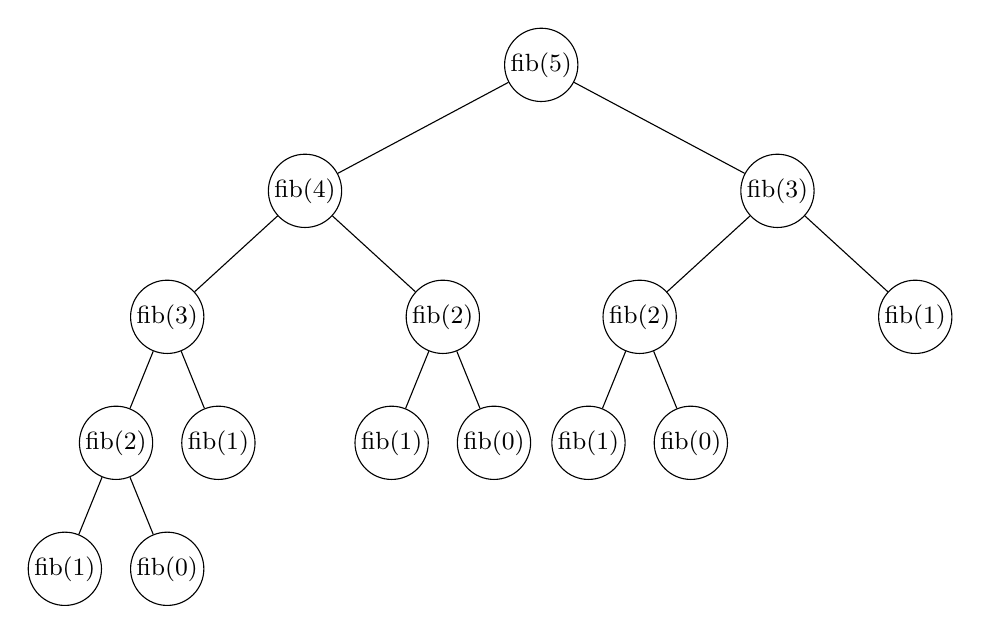
\begin{tikzpicture}[
    grow=down,
    level distance=1.6cm,
    level 1/.style={sibling distance=6cm},
    level 2/.style={sibling distance=3.5cm},
    level 3/.style={sibling distance=1.3cm}, 
    every node/.style={
        circle,
        draw,
        minimum size=7mm,
        inner sep=1pt,
        font=\small
    },
    edge from parent/.style={draw,-}
]

\node {fib(5)}
    child { node {fib(4)}
        child { node {fib(3)}
            child { node {fib(2)}
                child { node {fib(1)}}
                child { node {fib(0)}}
            }
            child { node {fib(1)}}
        }
        child { node {fib(2)}
            child { node {fib(1)}}
            child { node {fib(0)}}
        }
    }
    child { node {fib(3)}
        child { node {fib(2)}
            child { node {fib(1)}}
            child { node {fib(0)}}
        }
        child { node {fib(1)}}
    };

\end{tikzpicture}
\end{center}

\textbf{Notice:} We calculate \texttt{fib(3)} twice, \texttt{fib(2)} three times!

\begin{warning}
Time complexity: $O(2^n)$ — EXPONENTIAL!

\texttt{fib(40)} makes about 330 million function calls. \texttt{fib(50)} would take years!
\end{warning}

\subsection{The Solution: Memoization}

Remember results we've already computed:

\begin{lstlisting}
def fib_memo(n, memo={}):
    # Check if already computed
    if n in memo:
        return memo[n]
    
    # Base cases
    if n == 0:
        return 0
    if n == 1:
        return 1
    
    # Compute and store result
    memo[n] = fib_memo(n - 1, memo) + fib_memo(n - 2, memo)
    return memo[n]

print(fib_memo(50))  # Instant! 12586269025
\end{lstlisting}

\textbf{Time complexity:} $O(n)$ — each number computed once! \\
\textbf{Space complexity:} $O(n)$ — memo dictionary + call stack

\begin{keyidea}
\textbf{Memoization = Remember Results}

Store expensive function results. If called again with same input, return stored result instead of recomputing.

This turns exponential algorithms into polynomial ones!
\end{keyidea}

\section{Recursion with Multiple Branches: Tree Thinking}

\subsection{Example: Sum of Digits}

Find sum of all digits in a number. $1234 \to 1+2+3+4 = 10$

\begin{lstlisting}
def sum_of_digits(n):
    # Base case: single digit
    if n < 10:
        return n
    
    # Recursive case: last digit + sum of rest
    return (n % 10) + sum_of_digits(n // 10)

print(sum_of_digits(1234))  # 10
\end{lstlisting}

\textbf{How it works:}
\begin{align*}
\text{sum\_of\_digits}(1234) &= 4 + \text{sum\_of\_digits}(123) \\
&= 4 + (3 + \text{sum\_of\_digits}(12)) \\
&= 4 + (3 + (2 + \text{sum\_of\_digits}(1))) \\
&= 4 + (3 + (2 + 1)) \\
&= 10
\end{align*}

\section{Recursion on Arrays and Lists}

\subsection{Example 1: Find Maximum in Array}

\begin{lstlisting}
def find_max(arr, index=0):
    # Base case: last element
    if index == len(arr) - 1:
        return arr[index]
    
    # Recursive case: max of current vs max of rest
    max_of_rest = find_max(arr, index + 1)
    return max(arr[index], max_of_rest)

numbers = [3, 7, 2, 9, 1, 5]
print(find_max(numbers))  # 9
\end{lstlisting}

\subsection{Example 2: Reverse a String}

\begin{lstlisting}
def reverse_string(s):
    # Base case: empty or single character
    if len(s) <= 1:
        return s
    
    # Recursive case: last char + reverse of rest
    return s[-1] + reverse_string(s[:-1])

print(reverse_string("hello"))  # "olleh"
\end{lstlisting}

\textbf{Trace:}
\begin{align*}
\text{reverse}(\text{"hello"}) &= \text{"o"} + \text{reverse}(\text{"hell"}) \\
&= \text{"o"} + (\text{"l"} + \text{reverse}(\text{"hel"})) \\
&= \text{"o"} + (\text{"l"} + (\text{"l"} + \text{reverse}(\text{"he"}))) \\
&= \text{"o"} + (\text{"l"} + (\text{"l"} + (\text{"e"} + \text{reverse}(\text{"h"})))) \\
&= \text{"o"} + (\text{"l"} + (\text{"l"} + (\text{"e"} + \text{"h"}))) \\
&= \text{"olleh"}
\end{align*}

\section{Advanced: Tail Recursion}

\subsection{Regular Recursion (Work on the Way Back)}

\begin{lstlisting}
def factorial_regular(n):
    if n <= 1:
        return 1
    return n * factorial_regular(n - 1)  # Multiply AFTER return
\end{lstlisting}

Stack needs to remember $n$ for the multiplication after the recursive call returns.

\subsection{Tail Recursion (Work on the Way Down)}

\begin{lstlisting}
def factorial_tail(n, accumulator=1):
    if n <= 1:
        return accumulator
    return factorial_tail(n - 1, n * accumulator)  # Multiply BEFORE call

print(factorial_tail(5))  # 120
\end{lstlisting}

\begin{keyidea}
\textbf{Tail Recursion:} The recursive call is the last thing the function does (no work after it returns).

Some compilers can optimize this into a loop (called "tail call optimization"), saving stack space. Python doesn't do this, but other languages do!
\end{keyidea}

\section{The Recursion Tree: Visualizing Complexity}

For \texttt{fib(n)}, let's count function calls:

\begin{center}
\begin{tabular}{|c|c|c|}
\hline
$n$ & \textbf{Calls} & \textbf{Pattern} \\
\hline
0 & 1 & Base case \\
1 & 1 & Base case \\
2 & 3 & 1 + 1 + 1 \\
3 & 5 & 3 + 1 + 1 \\
4 & 9 & 5 + 3 + 1 \\
5 & 15 & 9 + 5 + 1 \\
$n$ & $\approx 2^n$ & Exponential! \\
\hline
\end{tabular}
\end{center}

\textbf{Height of tree:} $n$ \\
\textbf{Max nodes at each level:} $2^{\text{level}}$ \\
\textbf{Total nodes:} $O(2^n)$

\section{Practice Problems}

\subsection{Problem 1: Power Function}

Compute $x^n$ recursively.

\begin{lstlisting}
def power(x, n):
    """
    Compute x^n recursively.
    Example: power(2, 3) = 8
    """
    # Base case
    if n == 0:
        return 1
    
    # Recursive case
    return x * power(x, n - 1)

print(power(2, 10))  # 1024
\end{lstlisting}

\textbf{Optimization — Fast Power:}

\begin{lstlisting}
def fast_power(x, n):
    """
    Compute x^n in O(log n) time.
    Key insight: x^8 = (x^4)^2 = ((x^2)^2)^2
    """
    if n == 0:
        return 1
    
    if n % 2 == 0:
        # Even: x^n = (x^(n/2))^2
        half = fast_power(x, n // 2)
        return half * half
    else:
        # Odd: x^n = x * x^(n-1)
        return x * fast_power(x, n - 1)

print(fast_power(2, 10))  # 1024, but only 4 recursive calls!
\end{lstlisting}

\begin{keyidea}
Regular power: $O(n)$ multiplications \\
Fast power: $O(\log n)$ multiplications

For \texttt{power(2, 1000)}: \\
Regular: 1000 multiplications \\
Fast: Only 10 multiplications!
\end{keyidea}

\subsection{Problem 2: Check if String is Palindrome}

\begin{lstlisting}
def is_palindrome(s):
    """
    Check if string reads same forwards and backwards.
    Examples: "racecar" -> True, "hello" -> False
    """
    # Base case: 0 or 1 character
    if len(s) <= 1:
        return True
    
    # Check first and last characters
    if s[0] != s[-1]:
        return False
    
    # Recursively check the middle
    return is_palindrome(s[1:-1])

print(is_palindrome("racecar"))  # True
print(is_palindrome("hello"))    # False
print(is_palindrome("a"))        # True
\end{lstlisting}

\subsection{Problem 3: Generate All Permutations}

Generate all ways to arrange letters in a string.

\begin{lstlisting}
def permutations(s):
    """
    Generate all permutations of string s.
    Example: "abc" -> ["abc", "acb", "bac", "bca", "cab", "cba"]
    """
    # Base case: one character
    if len(s) <= 1:
        return [s]
    
    result = []
    
    # For each character, make it first, permute the rest
    for i in range(len(s)):
        first_char = s[i]
        remaining = s[:i] + s[i+1:]
        
        # Get all permutations of remaining characters
        for perm in permutations(remaining):
            result.append(first_char + perm)
    
    return result

print(permutations("abc"))
# ['abc', 'acb', 'bac', 'bca', 'cab', 'cba']
\end{lstlisting}

\textbf{Analysis:}
\begin{itemize}
    \item $n!$ permutations exist
    \item Each requires work to construct
    \item Time: $O(n \cdot n!)$
\end{itemize}

\section{Common Recursion Patterns}

\subsection{Pattern 1: Linear Recursion}

One recursive call per function call. Examples: factorial, countdown.
\begin{center}
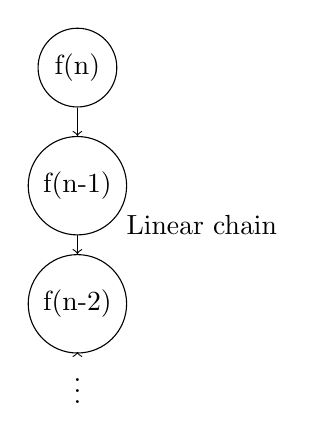
\begin{tikzpicture}
    \node[circle, draw, minimum size=1cm] (a) at (0,0) {f(n)};
    \node[circle, draw, minimum size=1cm] (b) at (0,-1.5) {f(n-1)};
    \node[circle, draw, minimum size=1cm] (c) at (0,-3) {f(n-2)};
    \node (d) at (0,-4) {$\vdots$};
    \draw[->] (a) -- (b);
    \draw[->] (b) -- (c);
    \draw[->] (c) -- (d);
    \node[right] at (0.5, -2) {Linear chain};
\end{tikzpicture}
\end{center}

\subsection{Pattern 2: Binary Recursion}

Two recursive calls. Examples: Fibonacci, binary tree traversal.

\begin{center}
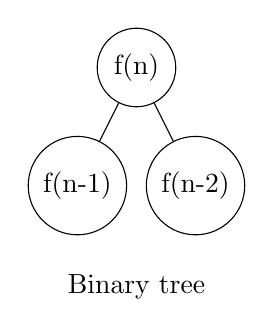
\begin{tikzpicture}[level distance=1.5cm]
    \node[circle, draw] {f(n)}
        child {node[circle, draw] {f(n-1)}}
        child {node[circle, draw] {f(n-2)}};
    
    \node[below] at (0, -2.5) {Binary tree};
\end{tikzpicture}
\end{center}

\subsection{Pattern 3: Multiple Recursion}

Many recursive calls. Example: tree with many branches.

\section{Debugging Recursive Functions}

\subsection{Tip 1: Add Print Statements}

\begin{lstlisting}
def factorial_debug(n, depth=0):
    indent = "  " * depth  # Indentation shows depth
    print(f"{indent}factorial({n}) called")
    
    if n <= 1:
        print(f"{indent}factorial({n}) returns 1")
        return 1
    
    result = n * factorial_debug(n - 1, depth + 1)
    print(f"{indent}factorial({n}) returns {result}")
    return result

factorial_debug(4)
\end{lstlisting}

\textbf{Output:}
\begin{verbatim}
factorial(4) called
  factorial(3) called
    factorial(2) called
      factorial(1) called
      factorial(1) returns 1
    factorial(2) returns 2
  factorial(3) returns 6
factorial(4) returns 24
\end{verbatim}

\subsection{Tip 2: Think in Terms of Trust}

When writing recursion:
\begin{enumerate}
    \item \textbf{Trust} that the recursive call works for smaller input
    \item Focus only on: base case + how to use the recursive result
    \item Don't try to trace the entire recursion in your head!
\end{enumerate}

\section{Key Takeaways}

\begin{enumerate}
    \item \textbf{Recursion = Self-Reference:} Function calls itself with smaller input
    
    \item \textbf{Must have Base Case:} Without it, infinite recursion!
    
    \item \textbf{Call Stack Remembers:} Each function call added to stack, removed when returns
    
    \item \textbf{Space Complexity:} Recursive functions use $O(\text{depth})$ stack space
    
    \item \textbf{When to Use:}
    \begin{itemize}
        \item Problem naturally recursive (trees, divide-and-conquer)
        \item Makes code much simpler and clearer
        \item Stack depth won't be excessive
    \end{itemize}
    
    \item \textbf{Memoization:} Remember results to avoid recomputation
    
    \item \textbf{Trace by Hand:} Best way to understand is to trace small examples
\end{enumerate}

\begin{insight}
Gilbert Strang's advice: "When learning recursion, start with the simplest examples. Trace them by hand. Draw the call stack. Only when you \textit{see} what's happening will the 'aha!' moment come. And when it does, recursion becomes your superpower for solving complex problems elegantly."
\end{insight}

\section{Looking Ahead to Chapter 4}

Now that you understand how functions work under the hood with the call stack, we're ready to use the stack as a \textbf{data structure} in its own right!

In Chapter 4, we'll explore \textbf{Stacks and Queues} — two fundamental data structures that model real-world scenarios like:
\begin{itemize}
    \item Browser back button (stack)
    \item Printer job queue (queue)  
    \item Expression evaluation (stack)
    \item Breadth-first search (queue)
\end{itemize}

Get ready — these are the building blocks of countless algorithms!

\vspace{1cm}

\begin{center}
\rule{0.5\textwidth}{0.4pt}

\textit{"Recursion is the art of solving problems by pretending they're already solved."}

\rule{0.5\textwidth}{0.4pt}
\end{center}
\pagebreak
\section{Chapter 4: Stacks and Queues}
\subsection*{The Two Most Natural Ways to Organize a Line}

\begin{center}
\textit{"A stack is a pile. A queue is a line. That's all you need to know to start."} 
\end{center}

\section{The Big Picture: Two Fundamental Orderings}

Think about real life:

\textbf{Stack of plates:} You add plates on top, remove from top. Last plate you put on is first one you take off.

\textbf{Line at a store:} People join at the back, leave from the front. First person in line is first to be served.

These are the TWO fundamental ways to order things:
\begin{itemize}
    \item \textbf{LIFO:} Last In, First Out (Stack)
    \item \textbf{FIFO:} First In, First Out (Queue)
\end{itemize}

\begin{insight}
Everything in computer science that involves ordering or sequencing comes down to these two patterns. Master stacks and queues, and you've mastered the foundation of algorithms.
\end{insight}

\section{Part I: THE STACK}

\subsection{First Principles: What IS a Stack?}

A stack is a collection where you can only:
\begin{enumerate}
    \item \textbf{Push:} Add an item to the top
    \item \textbf{Pop:} Remove the item from the top
    \item \textbf{Peek/Top:} Look at the top item (without removing)
\end{enumerate}

That's it. You CANNOT:
\begin{itemize}
    \item Access the middle
    \item Remove from the bottom
    \item Insert in the middle
\end{itemize}

\begin{center}
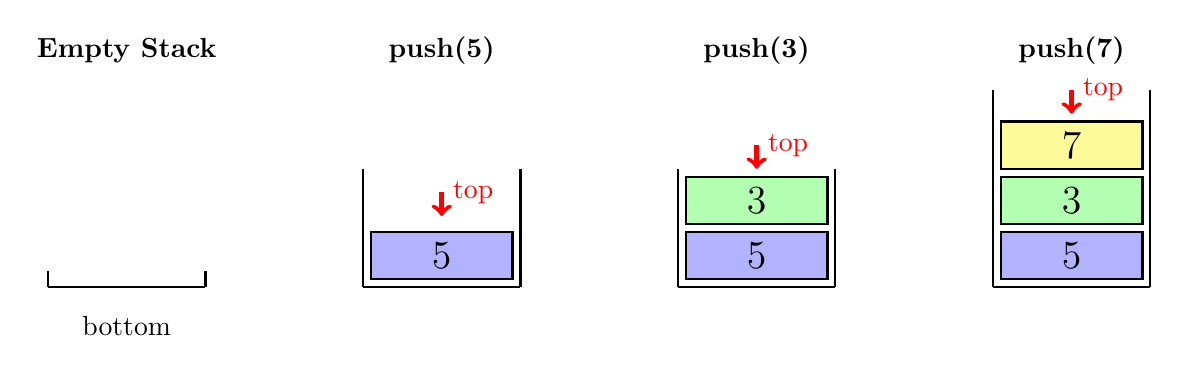
\begin{tikzpicture}[scale=1]
    % Empty stack
    \node at (-2, 3) {\textbf{Empty Stack}};
    \draw[thick] (-3, 0) -- (-1, 0);
    \draw[thick] (-3, 0) -- (-3, 0.2);
    \draw[thick] (-1, 0) -- (-1, 0.2);
    \node at (-2, -0.5) {bottom};
    
    % After push(5)
    \node at (2, 3) {\textbf{push(5)}};
    \draw[thick] (1, 0) -- (3, 0);
    \draw[thick] (1, 0) -- (1, 1.5);
    \draw[thick] (3, 0) -- (3, 1.5);
    \draw[thick, fill=blue!30] (1.1, 0.1) rectangle (2.9, 0.7);
    \node at (2, 0.4) {\Large 5};
    \draw[->, ultra thick, red] (2, 1.2) -- (2, 0.9);
    \node[red] at (2.4, 1.2) {top};
    
    % After push(3)
    \node at (6, 3) {\textbf{push(3)}};
    \draw[thick] (5, 0) -- (7, 0);
    \draw[thick] (5, 0) -- (5, 1.5);
    \draw[thick] (7, 0) -- (7, 1.5);
    \draw[thick, fill=blue!30] (5.1, 0.1) rectangle (6.9, 0.7);
    \node at (6, 0.4) {\Large 5};
    \draw[thick, fill=green!30] (5.1, 0.8) rectangle (6.9, 1.4);
    \node at (6, 1.1) {\Large 3};
    \draw[->, ultra thick, red] (6, 1.8) -- (6, 1.5);
    \node[red] at (6.4, 1.8) {top};
    
    % After push(7)
    \node at (10, 3) {\textbf{push(7)}};
    \draw[thick] (9, 0) -- (11, 0);
    \draw[thick] (9, 0) -- (9, 2.5);
    \draw[thick] (11, 0) -- (11, 2.5);
    \draw[thick, fill=blue!30] (9.1, 0.1) rectangle (10.9, 0.7);
    \node at (10, 0.4) {\Large 5};
    \draw[thick, fill=green!30] (9.1, 0.8) rectangle (10.9, 1.4);
    \node at (10, 1.1) {\Large 3};
    \draw[thick, fill=yellow!40] (9.1, 1.5) rectangle (10.9, 2.1);
    \node at (10, 1.8) {\Large 7};
    \draw[->, ultra thick, red] (10, 2.5) -- (10, 2.2);
    \node[red] at (10.4, 2.5) {top};
\end{tikzpicture}
\end{center}

\begin{center}
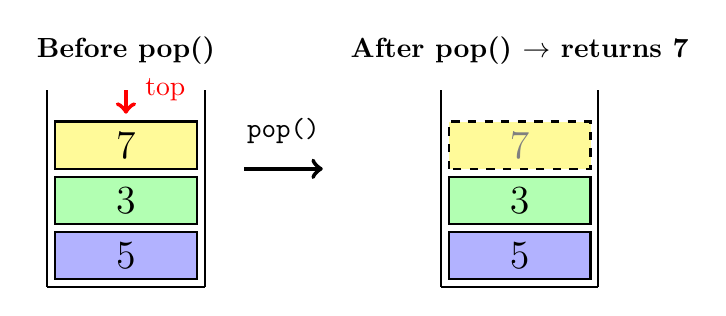
\begin{tikzpicture}[scale=1]
    % Before pop
    \node at (2, 3) {\textbf{Before pop()}};
    \draw[thick] (1, 0) -- (3, 0);
    \draw[thick] (1, 0) -- (1, 2.5);
    \draw[thick] (3, 0) -- (3, 2.5);
    \draw[thick, fill=blue!30] (1.1, 0.1) rectangle (2.9, 0.7);
    \node at (2, 0.4) {\Large 5};
    \draw[thick, fill=green!30] (1.1, 0.8) rectangle (2.9, 1.4);
    \node at (2, 1.1) {\Large 3};
    \draw[thick, fill=yellow!40] (1.1, 1.5) rectangle (2.9, 2.1);
    \node at (2, 1.8) {\Large 7};
    \draw[->, ultra thick, red] (2, 2.5) -- (2, 2.2);
    \node[red] at (2.5, 2.5) {top};
    
    % Arrow
    \draw[->, ultra thick] (3.5, 1.5) -- (4.5, 1.5);
    \node[above] at (4, 1.7) {\texttt{pop()}};
    
    % After pop (returns 7)
    \node at (7, 3) {\textbf{After pop() $\to$ returns 7}};
    \draw[thick] (6, 0) -- (8, 0);
    \draw[thick] (6, 0) -- (6, 2.5);
    \draw[thick] (8, 0) -- (8, 2.5);
    \draw[thick, fill=blue!30] (6.1, 0.1) rectangle (7.9, 0.7);
    \node at (7, 0.4) {\Large 5};
    \draw[thick, fill=green!30] (6.1, 0.8) rectangle (7.9, 1.4);
    \node at (7, 1.1) {\Large 3};
    \draw[->, ultra thick, red] (7, 1.8) -- (7, 1.5);
    \node[red] at (7.5, 1.8) {top};
    
    % Show removed element
    \draw[thick, fill=yellow!40, dashed] (6.1, 1.5) rectangle (7.9, 2.1);
    \node[gray] at (7, 1.8) {\Large 7};
\end{tikzpicture}
\end{center}

\begin{keyidea}
\textbf{The Stack Property:} The most recently added item is the first one removed.

Think of it as a \textbf{reversing mechanism} — whatever order things go in, they come out in REVERSE order.
\end{keyidea}

\subsection{Stack Implementation in Python}

Python lists make perfect stacks!

\begin{lstlisting}
class Stack:
    def __init__(self):
        self.items = []  # Use list as underlying storage
    
    def push(self, item):
        """Add item to top of stack"""
        self.items.append(item)  # O(1) amortized
    
    def pop(self):
        """Remove and return top item"""
        if self.is_empty():
            raise IndexError("Pop from empty stack")
        return self.items.pop()  # O(1)
    
    def peek(self):
        """Return top item without removing"""
        if self.is_empty():
            raise IndexError("Peek from empty stack")
        return self.items[-1]  # O(1)
    
    def is_empty(self):
        """Check if stack is empty"""
        return len(self.items) == 0  # O(1)
    
    def size(self):
        """Return number of items"""
        return len(self.items)  # O(1)
    
    def __str__(self):
        """String representation (top to bottom)"""
        return " <- ".join(str(item) for item in reversed(self.items))

# Let's use it!
stack = Stack()
stack.push(5)
stack.push(3)
stack.push(7)
print(stack)  # 7 <- 3 <- 5 (top to bottom)

print(stack.pop())  # 7
print(stack.peek()) # 3 (doesn't remove)
print(stack.pop())  # 3
\end{lstlisting}

\textbf{All operations are $O(1)$ — constant time!}

\subsection{Why Does This Matter? Real Applications}

\subsubsection{Application 1: Undo Functionality}

Every time you make a change, push it onto a stack:

\begin{lstlisting}
class TextEditor:
    def __init__(self):
        self.text = ""
        self.undo_stack = Stack()
    
    def write(self, new_text):
        # Save current state before modifying
        self.undo_stack.push(self.text)
        self.text = new_text
    
    def undo(self):
        if not self.undo_stack.is_empty():
            self.text = self.undo_stack.pop()

# Try it
editor = TextEditor()
editor.write("Hello")
editor.write("Hello World")
editor.write("Hello World!")
print(editor.text)  # "Hello World!"

editor.undo()
print(editor.text)  # "Hello World"

editor.undo()
print(editor.text)  # "Hello"
\end{lstlisting}

\subsubsection{Application 2: Balanced Parentheses}

Check if brackets are properly matched: \texttt{(([])\{\})} is valid, \texttt{([)] } is not.

\begin{lstlisting}
def is_balanced(expression):
    """
    Check if parentheses/brackets/braces are balanced.
    Examples:
        "(())" -> True
        "([)]" -> False
        "{[()]}" -> True
    """
    stack = Stack()
    matching = {'(': ')', '[': ']', '{': '}'}
    
    for char in expression:
        if char in matching:  # Opening bracket
            stack.push(char)
        elif char in matching.values():  # Closing bracket
            if stack.is_empty():
                return False  # Closing with no opening
            if matching[stack.pop()] != char:
                return False  # Mismatched pair
    
    return stack.is_empty()  # All opened should be closed

# Tests
print(is_balanced("((()))"))     # True
print(is_balanced("([{}])"))     # True
print(is_balanced("([)]"))       # False
print(is_balanced("((()"))       # False
\end{lstlisting}

\begin{center}
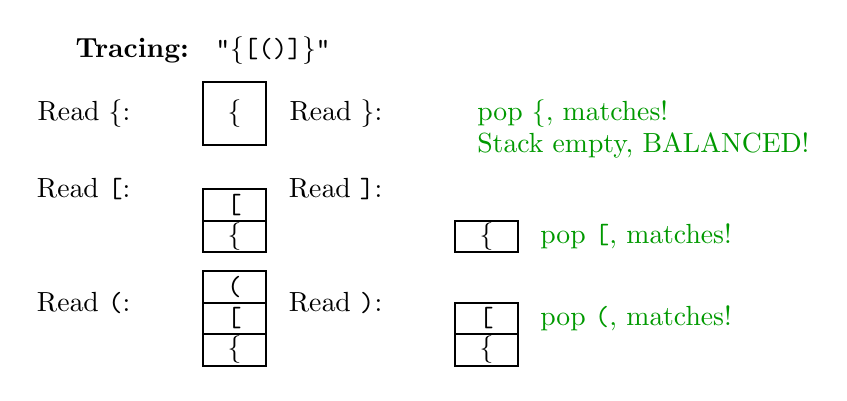
\begin{tikzpicture}[scale=0.8]
    \node at (0, 3.5) {\textbf{Tracing: } \texttt{"\{[()]\}"}};
    
    % Step by step
    \node[left] at (-1, 2.5) {Read \texttt{\{}:};
    \draw[thick] (0, 2) rectangle (1, 3);
    \node at (0.5, 2.5) {\texttt{\{}};
    
    \node[left] at (-1, 1.3) {Read \texttt{[}:};
    \draw[thick] (0, 0.3) rectangle (1, 0.8);
    \node at (0.5, 0.55) {\texttt{\{}};
    \draw[thick] (0, 0.8) rectangle (1, 1.3);
    \node at (0.5, 1.05) {\texttt{[}};
    
    \node[left] at (-1, -0.5) {Read \texttt{(}:};
    \draw[thick] (0, -1.5) rectangle (1, -1);
    \node at (0.5, -1.25) {\texttt{\{}};
    \draw[thick] (0, -1) rectangle (1, -0.5);
    \node at (0.5, -0.75) {\texttt{[}};
    \draw[thick] (0, -0.5) rectangle (1, 0);
    \node at (0.5, -0.25) {\texttt{(}};
    
    \node[left] at (3, -0.5) {Read \texttt{)}:};
    \draw[thick] (4, -1.5) rectangle (5, -1);
    \node at (4.5, -1.25) {\texttt{\{}};
    \draw[thick] (4, -1) rectangle (5, -0.5);
    \node at (4.5, -0.75) {\texttt{[}};
    \node[right, green!60!black] at (5.2, -0.75) {pop \texttt{(}, matches!};
    
    \node[left] at (3, 1.3) {Read \texttt{]}:};
    \draw[thick] (4, 0.3) rectangle (5, 0.8);
    \node at (4.5, 0.55) {\texttt{\{}};
    \node[right, green!60!black] at (5.2, 0.55) {pop \texttt{[}, matches!};
    
    \node[left] at (3, 2.5) {Read \texttt{\}}:};
    \node[right, green!60!black] at (4.2, 2.5) {pop \texttt{\{}, matches!};
    \node[right, green!60!black] at (4.2, 2) {Stack empty, BALANCED!};
\end{tikzpicture}
\end{center}

\begin{insight}
Why does a stack work here? Because brackets must be closed in REVERSE order of opening! The last opened bracket must be the first closed. That's exactly what a stack does.
\end{insight}

\subsubsection{Application 3: Evaluating Expressions}

Convert infix notation \texttt{3 + 4 * 2} to postfix \texttt{3 4 2 * +} using stacks.

\textbf{Postfix evaluation is simple:}

\begin{lstlisting}
def evaluate_postfix(expression):
    """
    Evaluate postfix expression.
    Example: "3 4 2 * +" means 3 + (4 * 2) = 11
    """
    stack = Stack()
    
    for token in expression.split():
        if token.isdigit():
            stack.push(int(token))
        else:  # It's an operator
            # Pop two operands (note the order!)
            right = stack.pop()
            left = stack.pop()
            
            # Apply operator
            if token == '+':
                result = left + right
            elif token == '-':
                result = left - right
            elif token == '*':
                result = left * right
            elif token == '/':
                result = left // right
            
            # Push result back
            stack.push(result)
    
    return stack.pop()

print(evaluate_postfix("3 4 2 * +"))  # 11
print(evaluate_postfix("5 1 2 + 4 * + 3 -"))  # 14
\end{lstlisting}
\begin{center}
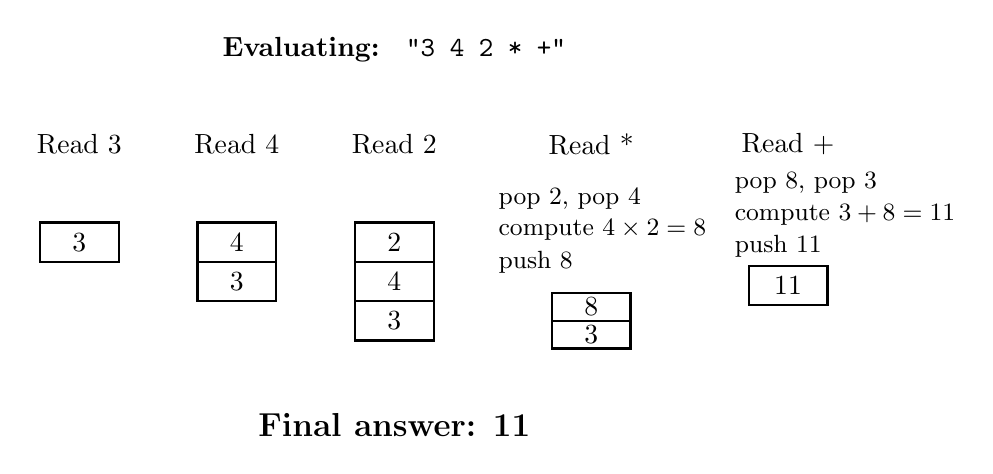
\begin{tikzpicture}[scale=1.0]
    \node at (5, 6.7) {\textbf{Evaluating: } \texttt{"3 4 2 * +"}};
    
    % Read 3
    \node at (1, 5.5) {Read 3};
    \draw[thick] (0.5, 4) rectangle (1.5, 4.5);
    \node at (1, 4.25) {3};
    
    % Read 4
    \node at (3, 5.5) {Read 4};
    \draw[thick] (2.5, 3.5) rectangle (3.5, 4);
    \node at (3, 3.75) {3};
    \draw[thick] (2.5, 4) rectangle (3.5, 4.5);
    \node at (3, 4.25) {4};
    
    % Read 2
    \node at (5, 5.5) {Read 2};
    \draw[thick] (4.5, 3) rectangle (5.5, 3.5);
    \node at (5, 3.25) {3};
    \draw[thick] (4.5, 3.5) rectangle (5.5, 4);
    \node at (5, 3.75) {4};
    \draw[thick] (4.5, 4) rectangle (5.5, 4.5);
    \node at (5, 4.25) {2};
    
    % Read *
    \node at (7.5, 5.5) {Read *};
    \node[font=\small, anchor=west] at (6.2, 4.8) {pop 2, pop 4};
    \node[font=\small, anchor=west] at (6.2, 4.4) {compute $4 \times 2 = 8$};
    \node[font=\small, anchor=west] at (6.2, 4.0) {push 8};
    \begin{scope}[yshift=-0.25cm]  % change this value to move more/less
        % Bottom rectangle
        \draw[thick] (7, 3.15) rectangle (8, 3.50);
        \node at (7.5, 3.325) {3};

        % Top rectangle
        \draw[thick] (7, 3.50) rectangle (8, 3.85);
        \node at (7.5, 3.675) {8};
    \end{scope}

    % Read +
    \node at (10, 5.5) {Read +};
    \node[font=\small, anchor=west] at (9.2, 5.0) {pop 8, pop 3};
    \node[font=\small, anchor=west] at (9.2, 4.6) {compute $3 + 8 = 11$};
    \node[font=\small, anchor=west] at (9.2, 4.2) {push 11};
    \draw[thick] (9.5, 3.45) rectangle (10.5, 3.95);
    \node at (10, 3.70) {11};

    
    \node[below, font=\large] at (5, 2.2) {\textbf{Final answer: 11}};
\end{tikzpicture}
\end{center}

\section{Part II: THE QUEUE}

\subsection{First Principles: What IS a Queue?}

A queue is a line where:
\begin{enumerate}
    \item \textbf{Enqueue:} Add item to the back/rear
    \item \textbf{Dequeue:} Remove item from the front
    \item \textbf{Peek/Front:} Look at front item (without removing)
\end{enumerate}

\begin{center}
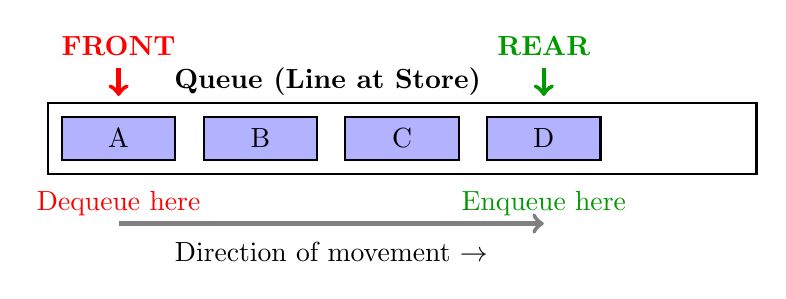
\begin{tikzpicture}[scale=0.9]
    % Queue representation
    \node at (3.95, 2.8) {\textbf{Queue (Line at Store)}};
    
    \draw[thick] (0, 1.5) rectangle (10, 2.5);
    
    % People in queue
    \draw[thick, fill=blue!30] (0.2, 1.7) rectangle (1.8, 2.3);
    \node at (1, 2) {A};
    
    \draw[thick, fill=blue!30] (2.2, 1.7) rectangle (3.8, 2.3);
    \node at (3, 2) {B};
    
    \draw[thick, fill=blue!30] (4.2, 1.7) rectangle (5.8, 2.3);
    \node at (5, 2) {C};
    
    \draw[thick, fill=blue!30] (6.2, 1.7) rectangle (7.8, 2.3);
    \node at (7, 2) {D};
    
    % Front and rear labels
    \draw[->, ultra thick, red] (1, 3) -- (1, 2.6);
    \node[red] at (1, 3.3) {\textbf{FRONT}};
    \node[red, below] at (1, 1.4) {Dequeue here};
    
    \draw[->, ultra thick, green!60!black] (7, 3) -- (7, 2.6);
    \node[green!60!black] at (7, 3.3) {\textbf{REAR}};
    \node[green!60!black, below] at (7, 1.4) {Enqueue here};
    
    % Show direction
    \draw[->, ultra thick, gray] (1, 0.8) -- (7, 0.8);
    \node at (4, 0.4) {Direction of movement $\to$};
\end{tikzpicture}
\end{center}

\begin{keyidea}
\textbf{The Queue Property:} First person in line is first person served.

Think of it as a \textbf{fair ordering mechanism} — no cutting in line! Items are processed in the exact order they arrive.
\end{keyidea}

\subsection{Queue Operations Visualized}

\begin{center}
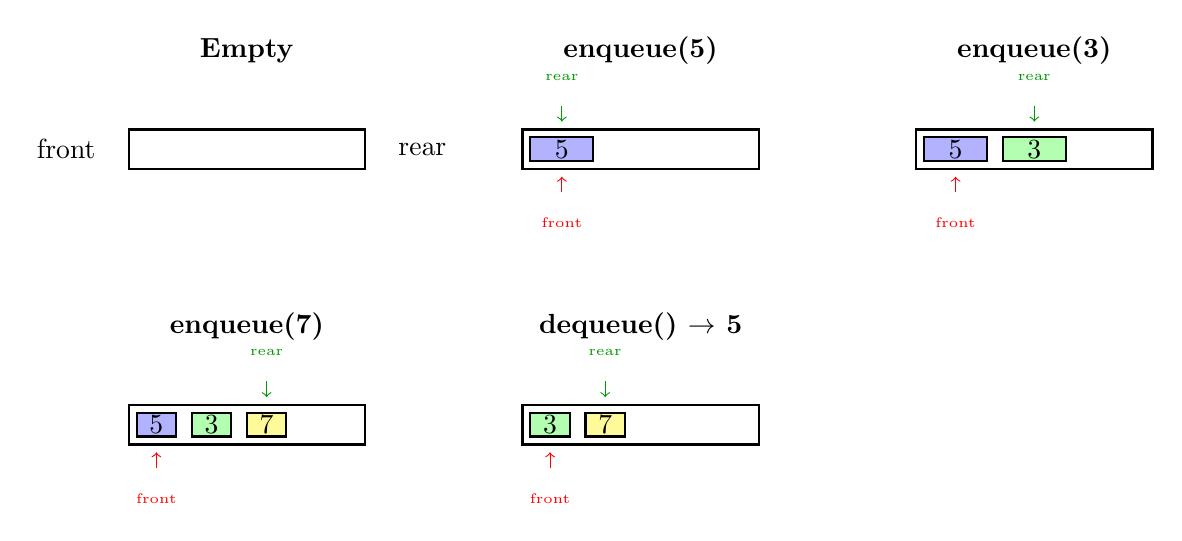
\begin{tikzpicture}[scale=1.0]
    % Empty queue
    \node at (1.5, 4) {\textbf{Empty}};
    \draw[thick] (0, 2.5) rectangle (3, 3);
    \node[left] at (-0.3, 2.75) {front};
    \node[right] at (3.3, 2.75) {rear};
    
    % After enqueue(5)
    \node at (6.5, 4) {\textbf{enqueue(5)}};
    \draw[thick] (5, 2.5) rectangle (8, 3);
    \draw[thick, fill=blue!30] (5.1, 2.6) rectangle (5.9, 2.9);
    \node at (5.5, 2.75) {5};
    \draw[->, red] (5.5, 2.2) -- (5.5, 2.4);
    \node[red, below, font=\tiny] at (5.5, 2) {front};
    \draw[->, green!60!black] (5.5, 3.3) -- (5.5, 3.1);
    \node[green!60!black, above, font=\tiny] at (5.5, 3.5) {rear};
    
    % After enqueue(3)
    \node at (11.5, 4) {\textbf{enqueue(3)}};
    \draw[thick] (10, 2.5) rectangle (13, 3);
    \draw[thick, fill=blue!30] (10.1, 2.6) rectangle (10.9, 2.9);
    \node at (10.5, 2.75) {5};
    \draw[thick, fill=green!30] (11.1, 2.6) rectangle (11.9, 2.9);
    \node at (11.5, 2.75) {3};
    \draw[->, red] (10.5, 2.2) -- (10.5, 2.4);
    \node[red, below, font=\tiny] at (10.5, 2) {front};
    \draw[->, green!60!black] (11.5, 3.3) -- (11.5, 3.1);
    \node[green!60!black, above, font=\tiny] at (11.5, 3.5) {rear};
    
    % After enqueue(7)
    \node at (1.5, 0.5) {\textbf{enqueue(7)}};
    \draw[thick] (0, -1) rectangle (3, -0.5);
    \draw[thick, fill=blue!30] (0.1, -0.9) rectangle (0.6, -0.6);
    \node at (0.35, -0.75) {5};
    \draw[thick, fill=green!30] (0.8, -0.9) rectangle (1.3, -0.6);
    \node at (1.05, -0.75) {3};
    \draw[thick, fill=yellow!40] (1.5, -0.9) rectangle (2.0, -0.6);
    \node at (1.75, -0.75) {7};
    \draw[->, red] (0.35, -1.3) -- (0.35, -1.1);
    \node[red, below, font=\tiny] at (0.35, -1.5) {front};
    \draw[->, green!60!black] (1.75, -0.2) -- (1.75, -0.4);
    \node[green!60!black, above, font=\tiny] at (1.75, 0) {rear};
    
    % After dequeue
    \node at (6.5, 0.5) {\textbf{dequeue() $\to$ 5}};
    \draw[thick] (5, -1) rectangle (8, -0.5);
    \draw[thick, fill=green!30] (5.1, -0.9) rectangle (5.6, -0.6);
    \node at (5.35, -0.75) {3};
    \draw[thick, fill=yellow!40] (5.8, -0.9) rectangle (6.3, -0.6);
    \node at (6.05, -0.75) {7};
    \draw[->, red] (5.35, -1.3) -- (5.35, -1.1);
    \node[red, below, font=\tiny] at (5.35, -1.5) {front};
    \draw[->, green!60!black] (6.05, -0.2) -- (6.05, -0.4);
    \node[green!60!black, above, font=\tiny] at (6.05, 0) {rear};
\end{tikzpicture}
\end{center}

\subsection{Queue Implementation Using List}

\begin{lstlisting}
class Queue:
    def __init__(self):
        self.items = []
    
    def enqueue(self, item):
        """Add item to rear of queue"""
        self.items.append(item)  # O(1) amortized
    
    def dequeue(self):
        """Remove and return front item"""
        if self.is_empty():
            raise IndexError("Dequeue from empty queue")
        return self.items.pop(0)  # O(n) - SLOW!
    
    def front(self):
        """Return front item without removing"""
        if self.is_empty():
            raise IndexError("Front from empty queue")
        return self.items[0]  # O(1)
    
    def is_empty(self):
        return len(self.items) == 0
    
    def size(self):
        return len(self.items)
    
    def __str__(self):
        return " <- ".join(str(item) for item in self.items)

# Usage
queue = Queue()
queue.enqueue(5)
queue.enqueue(3)
queue.enqueue(7)
print(queue)  # 5 <- 3 <- 7 (front to rear)

print(queue.dequeue())  # 5 (first in, first out!)
print(queue.front())    # 3
\end{lstlisting}

\begin{warning}
\textbf{Problem:} \texttt{pop(0)} is $O(n)$ because it shifts all remaining elements!

For a real queue, we need a better implementation...
\end{warning}

\subsection{Better Queue: Using collections.deque}

Python's \texttt{deque} (double-ended queue) is optimized for both ends:

\begin{lstlisting}
from collections import deque

class Queue:
    def __init__(self):
        self.items = deque()  # O(1) operations on both ends!
    
    def enqueue(self, item):
        self.items.append(item)  # O(1)
    
    def dequeue(self):
        if self.is_empty():
            raise IndexError("Dequeue from empty queue")
        return self.items.popleft()  # O(1) - FAST!
    
    def front(self):
        if self.is_empty():
            raise IndexError("Front from empty queue")
        return self.items[0]  # O(1)
    
    def is_empty(self):
        return len(self.items) == 0
    
    def size(self):
        return len(self.items)

# Now all operations are O(1)!
\end{lstlisting}

\section{Queue Applications: Where FIFO Matters}

\subsection{Application 1: Print Queue}

Documents are printed in order of submission:

\begin{lstlisting}
class PrintQueue:
    def __init__(self):
        self.queue = Queue()
    
    def add_job(self, document):
        """Submit a print job"""
        print(f"Adding to queue: {document}")
        self.queue.enqueue(document)
    
    def print_next(self):
        """Print the next document"""
        if not self.queue.is_empty():
            doc = self.queue.dequeue()
            print(f"Printing: {doc}")
        else:
            print("Queue is empty!")

# Simulate printer
printer = PrintQueue()
printer.add_job("Report.pdf")
printer.add_job("Resume.docx")
printer.add_job("Photo.jpg")

printer.print_next()  # Prints: Report.pdf (first in)
printer.print_next()  # Prints: Resume.docx
printer.print_next()  # Prints: Photo.jpg (last in)
\end{lstlisting}

\subsection{Application 2: Breadth-First Search (Preview)}

When exploring a graph or tree level by level, use a queue:

\begin{lstlisting}
def bfs_tree_levels(root):
    """
    Visit tree level by level (we'll learn trees later!)
    For now, just see how queue ensures level-order.
    """
    if not root:
        return
    
    queue = Queue()
    queue.enqueue(root)
    
    while not queue.is_empty():
        node = queue.dequeue()  # Process front node
        print(node.value)
        
        # Add children to queue (rear)
        if node.left:
            queue.enqueue(node.left)
        if node.right:
            queue.enqueue(node.right)
    
    # Result: level 1, then level 2, then level 3, etc.
\end{lstlisting}

\begin{center}
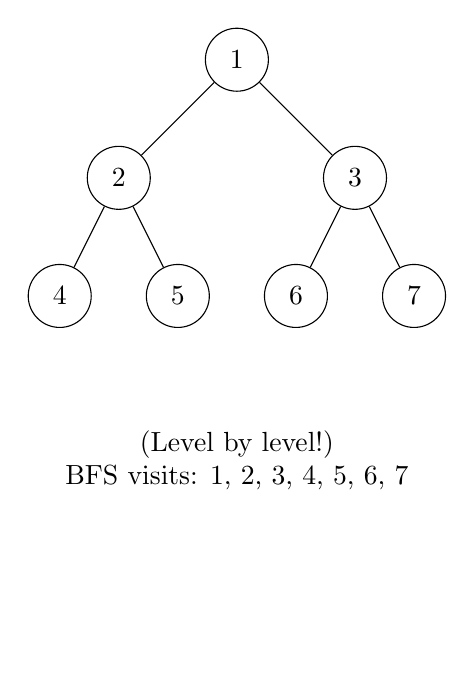
\begin{tikzpicture}[
    level distance=1.5cm,
    level 1/.style={sibling distance=3cm},
    level 2/.style={sibling distance=1.5cm},
    every node/.style={circle, draw, minimum size=0.8cm}
]

\node {1}
    child {node {2}
        child {node {4}}
        child {node {5}}
    }
    child {node {3}
        child {node {6}}
        child {node {7}}
    };

\node[below, draw=none] at (0, -3) {BFS visits: 1, 2, 3, 4, 5, 6, 7};
\node[below, draw=none] at (0, -3.5) {(Level by level!)};

\end{tikzpicture}
\end{center}

\section{Stack vs Queue: Side by Side Comparison}

\begin{center}
\begin{tabular}{|l|c|c|}
\hline
\textbf{Property} & \textbf{Stack} & \textbf{Queue} \\
\hline
Order & LIFO & FIFO \\
\hline
Add & Push (top) & Enqueue (rear) \\
\hline
Remove & Pop (top) & Dequeue (front) \\
\hline
Real-world & Plates, Undo & Line, Print jobs \\
\hline
Use when & Reverse order & Preserve order \\
\hline
Algorithm & DFS, Recursion & BFS, Scheduling \\
\hline
\end{tabular}
\end{center}

\begin{insight}
\textbf{Strang's Rule of Thumb:}

\begin{itemize}
    \item Need to \textbf{backtrack} or \textbf{reverse}? $\to$ Stack
    \item Need to \textbf{process in order} or go \textbf{level by level}? $\to$ Queue
\end{itemize}

Once you understand these two patterns, you'll recognize them everywhere in algorithms!
\end{insight}

\section{Practice Problems}

\subsection{Problem 1: Implement Stack Using Queues}

Can you implement a stack using only queue operations?

\begin{lstlisting}
class StackUsingQueues:
    """
    Implement stack using two queues.
    Key insight: To reverse order, transfer between queues.
    """
    def __init__(self):
        self.q1 = Queue()
        self.q2 = Queue()
    
    def push(self, item):
        # Add to q2
        self.q2.enqueue(item)
        
        # Transfer all from q1 to q2 (reverses order!)
        while not self.q1.is_empty():
            self.q2.enqueue(self.q1.dequeue())
        
        # Swap q1 and q2
        self.q1, self.q2 = self.q2, self.q1
    
    def pop(self):
        if self.q1.is_empty():
            raise IndexError("Pop from empty stack")
        return self.q1.dequeue()
    
    def top(self):
        if self.q1.is_empty():
            raise IndexError("Top from empty stack")
        return self.q1.front()

# Test
stack = StackUsingQueues()
stack.push(1)
stack.push(2)
stack.push(3)
print(stack.pop())  # 3 (LIFO using queues!)
print(stack.top())  # 2
\end{lstlisting}

\subsection{Problem 2: Valid Parentheses (Extended)}

Now with multiple bracket types and better clarity:

\begin{lstlisting}
def is_valid_brackets(s):
    """
    Check if string has valid brackets.
    Valid: "()[]{}", "([{}])"
    Invalid: "([)]", "((("
    """
    stack = Stack()
    pairs = {'(': ')', '[': ']', '{': '}'}
    
    for char in s:
        if char in pairs:  # Opening bracket
            stack.push(char)
        elif char in pairs.values():  # Closing bracket
            if stack.is_empty():
                return False
            opening = stack.pop()
            if pairs[opening] != char:
                return False
    
    return stack.is_empty()

# Test cases
print(is_valid_brackets("()[]{}"))      # True
print(is_valid_brackets("([{}])"))      # True
print(is_valid_brackets("([)]"))        # False (wrong nesting)
print(is_valid_brackets("((()"))        # False (unclosed)
\end{lstlisting}

\subsection{Problem 3: Hot Potato Game (Circular Queue)}

Kids pass a potato in circle, every $k$-th person is out:

\begin{lstlisting}
def hot_potato(names, num):
    """
    Simulate hot potato game.
    Every 'num' passes, one person is eliminated.
    """
    queue = Queue()
    
    # Add all players to queue
    for name in names:
        queue.enqueue(name)
    
    # Play game
    while queue.size() > 1:
        # Pass potato 'num' times
        for _ in range(num):
            queue.enqueue(queue.dequeue())  # Move front to rear
        
        # Eliminate current front person
        eliminated = queue.dequeue()
        print(f"{eliminated} is out!")
    
    # Winner is last person remaining
    return queue.dequeue()

# Play!
players = ["Alice", "Bob", "Charlie", "David", "Eve"]
winner = hot_potato(players, 3)
print(f"Winner is: {winner}")
\end{lstlisting}

\textbf{Example run with num=3:}
\begin{verbatim}
Pass 3 times: Alice -> Bob -> Charlie (David eliminated)
Pass 3 times: Eve -> Alice -> Bob (Charlie eliminated)
Pass 3 times: Eve -> Alice (Bob eliminated)
Pass 3 times: Eve (Alice eliminated)
Winner: Eve
\end{verbatim}

\subsection{Problem 4: Reverse First K Elements of Queue}

\begin{lstlisting}
def reverse_first_k(queue, k):
    """
    Reverse first k elements of queue.
    Example: [1,2,3,4,5], k=3 -> [3,2,1,4,5]
    """
    if k > queue.size() or k <= 0:
        return
    
    stack = Stack()
    
    # Step 1: Move first k elements to stack (reverses them)
    for _ in range(k):
        stack.push(queue.dequeue())
    
    # Step 2: Move from stack back to queue (now reversed)
    while not stack.is_empty():
        queue.enqueue(stack.pop())
    
    # Step 3: Move remaining elements to back
    for _ in range(queue.size() - k):
        queue.enqueue(queue.dequeue())

# Test
q = Queue()
for i in [1, 2, 3, 4, 5]:
    q.enqueue(i)

reverse_first_k(q, 3)
# Queue is now: 3, 2, 1, 4, 5
\end{lstlisting}

\begin{keyidea}
This problem beautifully shows how stacks and queues complement each other:
\begin{itemize}
    \item Stack reverses order
    \item Queue preserves order
    \item Together, they can do complex rearrangements!
\end{itemize}
\end{keyidea}

\section{Double-Ended Queue (Deque): The Hybrid}

A \textbf{deque} can add/remove from BOTH ends:

\begin{center}
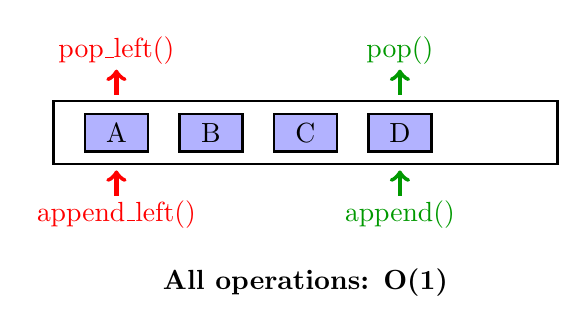
\begin{tikzpicture}[scale=0.8]
    \draw[thick] (0, 1) rectangle (8, 2);
    
    \draw[thick, fill=blue!30] (0.5, 1.2) rectangle (1.5, 1.8);
    \node at (1, 1.5) {A};
    
    \draw[thick, fill=blue!30] (2, 1.2) rectangle (3, 1.8);
    \node at (2.5, 1.5) {B};
    
    \draw[thick, fill=blue!30] (3.5, 1.2) rectangle (4.5, 1.8);
    \node at (4, 1.5) {C};
    
    \draw[thick, fill=blue!30] (5, 1.2) rectangle (6, 1.8);
    \node at (5.5, 1.5) {D};
    
    % Operations on both ends
    \draw[<-, ultra thick, red] (1, 2.5) -- (1, 2.1);
    \node[red] at (1, 2.8) {pop\_left()};
    \draw[->, ultra thick, red] (1, 0.5) -- (1, 0.9);
    \node[red] at (1, 0.2) {append\_left()};
    
    \draw[<-, ultra thick, green!60!black] (5.5, 2.5) -- (5.5, 2.1);
    \node[green!60!black] at (5.5, 2.8) {pop()};
    \draw[->, ultra thick, green!60!black] (5.5, 0.5) -- (5.5, 0.9);
    \node[green!60!black] at (5.5, 0.2) {append()};
    
    \node[below] at (4, -0.5) {\textbf{All operations: O(1)}};
\end{tikzpicture}
\end{center}

\begin{lstlisting}
from collections import deque

# Create deque
dq = deque([1, 2, 3])

# Stack operations (right end)
dq.append(4)        # [1, 2, 3, 4]
dq.pop()            # [1, 2, 3]

# Queue operations (left end)
dq.appendleft(0)    # [0, 1, 2, 3]
dq.popleft()        # [1, 2, 3]

# Both ends in O(1)! Best of both worlds!
\end{lstlisting}

\section{Key Takeaways}

\begin{enumerate}
    \item \textbf{Stack = LIFO:} Last In, First Out
    \begin{itemize}
        \item Use for: Undo, backtracking, reversing, DFS
        \item All operations: $O(1)$
    \end{itemize}
    
    \item \textbf{Queue = FIFO:} First In, First Out
    \begin{itemize}
        \item Use for: Order preservation, BFS, scheduling
        \item With deque: All operations $O(1)$
        \item With list: dequeue is $O(n)$ — use deque instead!
    \end{itemize}
    
    \item \textbf{Real-world analogies matter:}
    \begin{itemize}
        \item Stack = Pile of plates
        \item Queue = Line at store
    \end{itemize}
    
    \item \textbf{They're complements:}
    \begin{itemize}
        \item Stack reverses order
        \item Queue preserves order
        \item Deque does both
    \end{itemize}
    
    \item \textbf{Implementation matters:}
    \begin{itemize}
        \item Python list $\to$ good for stack
        \item Python deque $\to$ good for queue
        \item Choice affects performance!
    \end{itemize}
\end{enumerate}

\begin{insight}
Gilbert Strang would say: "These structures are so fundamental because they model the two most basic ways we think about order: most recent first, or first come first served. Everything else in computer science builds on these two simple ideas. Master them, and you've mastered the foundation."
\end{insight}

\section{Looking Ahead to Chapter 5}

Now that we understand how to organize data in lines (stacks and queues), we're ready for a completely different approach: \textbf{Linked Lists}.

What if items don't need to be in consecutive memory? What if each item could live anywhere and just "point" to the next one, like a treasure hunt?

That's the beauty of linked lists — flexibility at the cost of random access. Get ready for pointers!

\vspace{1cm}

\begin{center}
\rule{0.5\textwidth}{0.4pt}

\textit{"Stack and queue: Two simple ideas that power half of computer science."}

\rule{0.5\textwidth}{0.4pt}
\end{center}
\pagebreak
\section{Chapter 5: Linked Lists}
\subsection*{Freedom from Consecutive Memory}

\begin{center}
\textit{"An array is a street of houses. A linked list is a treasure hunt where each clue leads to the next."}
\end{center}

\section{The Big Picture: Why Do We Need Linked Lists?}

Remember arrays? They require consecutive memory blocks. This creates problems:

\begin{itemize}
    \item \textbf{Inserting in the middle:} Shift everything $\to$ $O(n)$
    \item \textbf{Growing the array:} Need to find bigger consecutive space, copy everything
    \item \textbf{Wasted space:} Must allocate more than needed for growth
\end{itemize}

\textbf{The Big Idea:} What if elements could live \textit{anywhere} in memory, and each element just remembers where the next one is?

\begin{keyidea}
\textbf{Linked List:} A sequence of nodes where each node contains:
\begin{enumerate}
    \item Data (the actual value)
    \item Pointer/Reference (address of the next node)
\end{enumerate}

Like a treasure hunt: Each clue tells you where to find the next clue!
\end{keyidea}

\section{First Principles: The Node}

\subsection{Understanding the Node}

A node is the basic building block:

\begin{center}
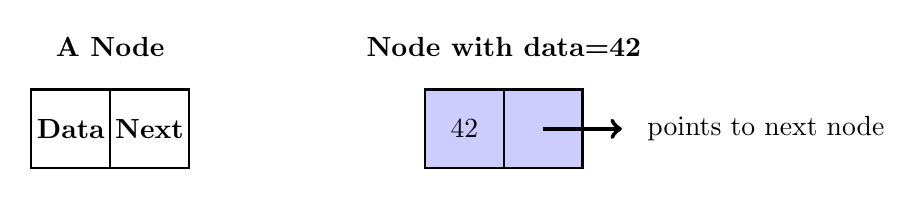
\begin{tikzpicture}[scale=1]
    % Single node structure
    \draw[thick] (0,0) rectangle (2,1);
    \draw[thick] (1,0) -- (1,1);
    
    \node at (0.5, 0.5) {\textbf{Data}};
    \node at (1.5, 0.5) {\textbf{Next}};
    
    \node[above] at (1, 1.3) {\textbf{A Node}};
    
    % Example node with value
    \draw[thick, fill=blue!20] (5,0) rectangle (7,1);
    \draw[thick] (6,0) -- (6,1);
    
    \node at (5.5, 0.5) {42};
    \draw[->, ultra thick] (6.5, 0.5) -- (7.5, 0.5);
    
    \node[above] at (6, 1.3) {\textbf{Node with data=42}};
    \node[right] at (7.7, 0.5) {points to next node};
\end{tikzpicture}
\end{center}

\subsection{Node Implementation in Python}

\begin{lstlisting}
class Node:
    def __init__(self, data):
        self.data = data    # Store the value
        self.next = None    # Initially doesn't point anywhere
    
    def __str__(self):
        return f"Node({self.data})"

# Create individual nodes
node1 = Node(10)
node2 = Node(20)
node3 = Node(30)

# Link them together
node1.next = node2  # node1 points to node2
node2.next = node3  # node2 points to node3
node3.next = None   # node3 is the last (points to nothing)

# Now we have a chain: 10 -> 20 -> 30 -> None
\end{lstlisting}

\subsection{Visualizing the Chain}

\begin{center}
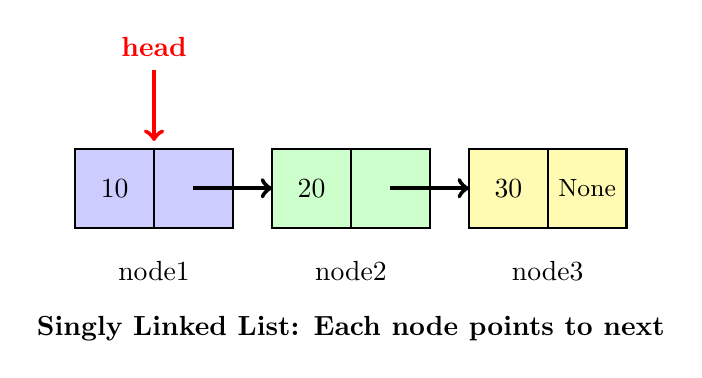
\begin{tikzpicture}[scale=1.0]
    % Node 1
    \draw[thick, fill=blue!20] (0,0) rectangle (2,1);
    \draw[thick] (1,0) -- (1,1);
    \node at (0.5, 0.5) {10};
    \draw[->, ultra thick] (1.5, 0.5) -- (2.5, 0.5);
    
    % Node 2
    \draw[thick, fill=green!20] (2.5,0) rectangle (4.5,1);
    \draw[thick] (3.5,0) -- (3.5,1);
    \node at (3, 0.5) {20};
    \draw[->, ultra thick] (4, 0.5) -- (5, 0.5);
    
    % Node 3
    \draw[thick, fill=yellow!30] (5,0) rectangle (7,1);
    \draw[thick] (6,0) -- (6,1);
    \node at (5.5, 0.5) {30};
    \node[font=\small] at (6.5, 0.5) {None};
    
    % Labels
    \node[below] at (1, -0.3) {node1};
    \node[below] at (3.5, -0.3) {node2};
    \node[below] at (6, -0.3) {node3};
    
    % Head pointer
    \draw[->, ultra thick, red] (1, 2) -- (1, 1.1);
    \node[red] at (1, 2.3) {\textbf{head}};
    
    \node[below] at (3.5, -1) {\textbf{Singly Linked List: Each node points to next}};
\end{tikzpicture}
\end{center}

\begin{insight}
\textbf{Key Insight:} We only need to remember the \textbf{head} (first node). From there, we can reach any other node by following the chain!

This is like knowing the entrance to a maze — you can find your way through by following the path.
\end{insight}

\section{Building a Linked List Class}

\subsection{The LinkedList Class}

\begin{lstlisting}
class LinkedList:
    def __init__(self):
        self.head = None  # Start with empty list
        self.size = 0
    
    def is_empty(self):
        """Check if list is empty"""
        return self.head is None
    
    def __len__(self):
        """Return size of list"""
        return self.size
    
    def __str__(self):
        """String representation: 1 -> 2 -> 3 -> None"""
        if self.is_empty():
            return "Empty List"
        
        result = []
        current = self.head
        while current is not None:
            result.append(str(current.data))
            current = current.next
        
        return " -> ".join(result) + " -> None"

# Create empty list
ll = LinkedList()
print(ll)  # Empty List
\end{lstlisting}

\section{Core Operations: Building Intuition}

\subsection{Operation 1: Insert at Beginning (Prepend)}

\textbf{Question:} How do we add a new node at the front?

\textbf{Steps:}
\begin{enumerate}
    \item Create new node
    \item Make new node point to current head
    \item Update head to be the new node
\end{enumerate}

\begin{center}
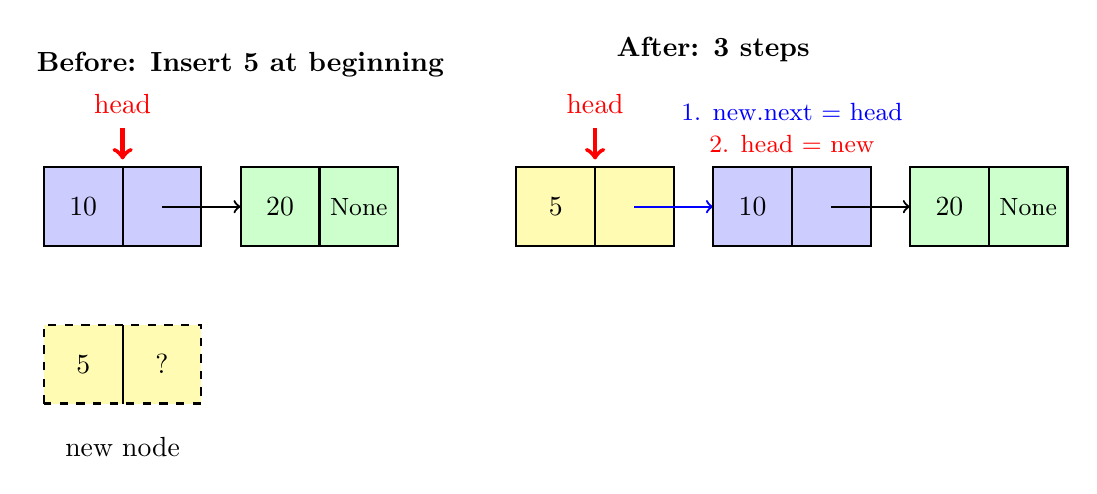
\begin{tikzpicture}[scale=1.0]
    % Before
    \node at (2.5, 5.3) {\textbf{Before: Insert 5 at beginning}};
    
    \draw[thick, fill=blue!20] (0,3) rectangle (2,4);
    \draw[thick] (1,3) -- (1,4);
    \node at (0.5, 3.5) {10};
    \draw[->, thick] (1.5, 3.5) -- (2.5, 3.5);
    
    \draw[thick, fill=green!20] (2.5,3) rectangle (4.5,4);
    \draw[thick] (3.5,3) -- (3.5,4);
    \node at (3, 3.5) {20};
    \node[font=\small] at (4, 3.5) {None};
    
    \draw[->, ultra thick, red] (1, 4.5) -- (1, 4.1);
    \node[red] at (1, 4.8) {head};
    
    % New node to be inserted
    \draw[thick, fill=yellow!30, dashed] (0,1) rectangle (2,2);
    \draw[thick] (1,1) -- (1,2);
    \node at (0.5, 1.5) {5};
    \node at (1.5, 1.5) {?};
    \node[below] at (1, 0.7) {new node};
    
    % After
    \node at (8.5, 5.5) {\textbf{After: 3 steps}};
    
    % Step 1: new node created
    \draw[thick, fill=yellow!30] (6,3) rectangle (8,4);
    \draw[thick] (7,3) -- (7,4);
    \node at (6.5, 3.5) {5};
    \draw[->, thick, blue] (7.5, 3.5) -- (8.5, 3.5);
    
    % Step 2: points to old head
    \draw[thick, fill=blue!20] (8.5,3) rectangle (10.5,4);
    \draw[thick] (9.5,3) -- (9.5,4);
    \node at (9, 3.5) {10};
    \draw[->, thick] (10, 3.5) -- (11, 3.5);
    
    \draw[thick, fill=green!20] (11,3) rectangle (13,4);
    \draw[thick] (12,3) -- (12,4);
    \node at (11.5, 3.5) {20};
    \node[font=\small] at (12.5, 3.5) {None};
    
    % Step 3: update head
    \draw[->, ultra thick, red] (7, 4.5) -- (7, 4.1);
    \node[red] at (7, 4.8) {head};
    
    % Labels
    \node[blue, font=\small] at (9.5, 4.7) {1. new.next = head};
    \node[red, font=\small] at (9.5, 4.3) {2. head = new};
\end{tikzpicture}
\end{center}

\begin{lstlisting}
def prepend(self, data):
    """Insert at beginning - O(1)"""
    new_node = Node(data)
    new_node.next = self.head  # Step 1: Point to old head
    self.head = new_node       # Step 2: Update head
    self.size += 1

# Usage
ll = LinkedList()
ll.prepend(20)  # List: 20 -> None
ll.prepend(10)  # List: 10 -> 20 -> None
ll.prepend(5)   # List: 5 -> 10 -> 20 -> None
print(ll)
\end{lstlisting}

\textbf{Time Complexity:} $O(1)$ — constant time! Just update a few pointers.

\begin{keyidea}
\textbf{Why is prepend so fast?}

In an array, inserting at the beginning requires shifting everything. In a linked list, we just:
\begin{itemize}
    \item Create new node
    \item Update two pointers
\end{itemize}

No shifting needed! This is the power of linked lists.
\end{keyidea}

\subsection{Operation 2: Insert at End (Append)}

\textbf{Problem:} To add at the end, we must walk through the entire list to find the last node.

\begin{center}
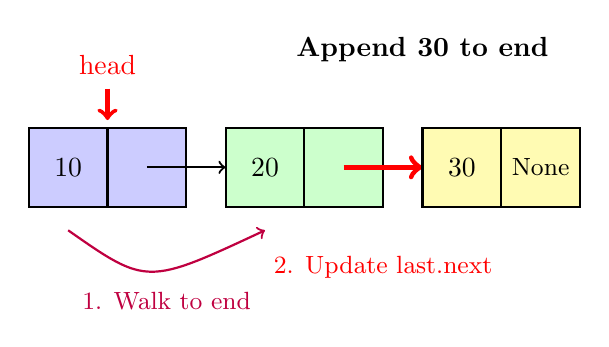
\begin{tikzpicture}[scale=1.0]
    \node at (5, 5) {\textbf{Append 30 to end}};
    
    % Existing list
    \draw[thick, fill=blue!20] (0,3) rectangle (2,4);
    \draw[thick] (1,3) -- (1,4);
    \node at (0.5, 3.5) {10};
    \draw[->, thick] (1.5, 3.5) -- (2.5, 3.5);
    
    \draw[thick, fill=green!20] (2.5,3) rectangle (4.5,4);
    \draw[thick] (3.5,3) -- (3.5,4);
    \node at (3, 3.5) {20};
    \draw[->, thick, red, line width=2pt] (4, 3.5) -- (5, 3.5);
    
    \draw[->, ultra thick, red] (1, 4.5) -- (1, 4.1);
    \node[red] at (1, 4.8) {head};
    
    % Traverse arrows
    \draw[->, thick, purple] (0.5, 2.7) .. controls (1.5, 2) .. (3, 2.7);
    \node[purple, font=\small] at (1.75, 1.8) {1. Walk to end};
    
    % New node
    \draw[thick, fill=yellow!30] (5,3) rectangle (7,4);
    \draw[thick] (6,3) -- (6,4);
    \node at (5.5, 3.5) {30};
    \node[font=\small] at (6.5, 3.5) {None};
    
    \node[red, below, font=\small] at (4.5, 2.5) {2. Update last.next};
\end{tikzpicture}
\end{center}

\begin{lstlisting}
def append(self, data):
    """Insert at end - O(n)"""
    new_node = Node(data)
    
    # Special case: empty list
    if self.is_empty():
        self.head = new_node
        self.size += 1
        return
    
    # Walk to the end
    current = self.head
    while current.next is not None:  # O(n) - must traverse
        current = current.next
    
    # Now current is the last node
    current.next = new_node
    self.size += 1

# Usage
ll = LinkedList()
ll.append(10)  # List: 10 -> None
ll.append(20)  # List: 10 -> 20 -> None
ll.append(30)  # List: 10 -> 20 -> 30 -> None
\end{lstlisting}

\textbf{Time Complexity:} $O(n)$ — must walk through entire list!

\begin{insight}
\textbf{Optimization:} Keep a \texttt{tail} pointer!

If we maintain a pointer to the last node, append becomes $O(1)$ too. This is a common optimization.
\end{insight}

\subsection{Operation 3: Delete a Node}

\textbf{Challenge:} To delete a node, we need to update the previous node's pointer to skip over it.

\begin{center}
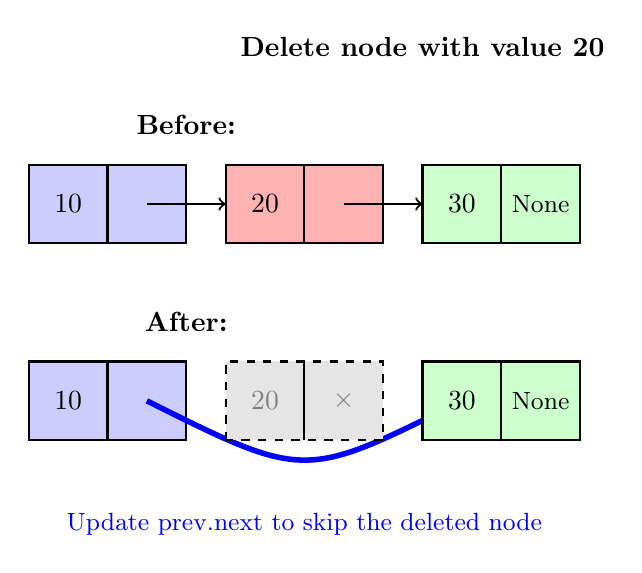
\begin{tikzpicture}[scale=1.0]
    \node at (5, 6) {\textbf{Delete node with value 20}};
    
    % Before
    \node at (2, 5) {\textbf{Before:}};
    \draw[thick, fill=blue!20] (0,3.5) rectangle (2,4.5);
    \draw[thick] (1,3.5) -- (1,4.5);
    \node at (0.5, 4) {10};
    \draw[->, thick] (1.5, 4) -- (2.5, 4);
    
    \draw[thick, fill=red!30] (2.5,3.5) rectangle (4.5,4.5);
    \draw[thick] (3.5,3.5) -- (3.5,4.5);
    \node at (3, 4) {20};
    \draw[->, thick] (4, 4) -- (5, 4);
    
    \draw[thick, fill=green!20] (5,3.5) rectangle (7,4.5);
    \draw[thick] (6,3.5) -- (6,4.5);
    \node at (5.5, 4) {30};
    \node[font=\small] at (6.5, 4) {None};
    
    % After
    \node at (2, 2.5) {\textbf{After:}};
    \draw[thick, fill=blue!20] (0,1) rectangle (2,2);
    \draw[thick] (1,1) -- (1,2);
    \node at (0.5, 1.5) {10};
    \draw[->, thick, blue, line width=2pt] (1.5, 1.5) .. controls (3.5, 0.5) .. (5.5, 1.5);
    
    \draw[thick, fill=green!20] (5,1) rectangle (7,2);
    \draw[thick] (6,1) -- (6,2);
    \node at (5.5, 1.5) {30};
    \node[font=\small] at (6.5, 1.5) {None};
    
    % Deleted node (grayed out)
    \draw[thick, fill=gray!20, dashed] (2.5,1) rectangle (4.5,2);
    \draw[thick] (3.5,1) -- (3.5,2);
    \node[gray] at (3, 1.5) {20};
    \node[gray] at (4, 1.5) {$\times$};
    
    \node[blue, below, font=\small] at (3.5, 0.2) {Update prev.next to skip the deleted node};
\end{tikzpicture}
\end{center}

\begin{lstlisting}
def delete(self, data):
    """Delete first occurrence of data - O(n)"""
    if self.is_empty():
        return False
    
    # Special case: delete head
    if self.head.data == data:
        self.head = self.head.next
        self.size -= 1
        return True
    
    # Find the node before the one to delete
    current = self.head
    while current.next is not None:
        if current.next.data == data:
            # Skip over the node to delete
            current.next = current.next.next
            self.size -= 1
            return True
        current = current.next
    
    return False  # Not found

# Usage
ll = LinkedList()
ll.append(10)
ll.append(20)
ll.append(30)
print(ll)  # 10 -> 20 -> 30 -> None

ll.delete(20)
print(ll)  # 10 -> 30 -> None
\end{lstlisting}

\textbf{Time Complexity:} $O(n)$ — must search for the node

\subsection{Operation 4: Search}

\begin{lstlisting}
def search(self, data):
    """Find if data exists in list - O(n)"""
    current = self.head
    while current is not None:
        if current.data == data:
            return True
        current = current.next
    return False

# Usage
print(ll.search(30))  # True
print(ll.search(99))  # False
\end{lstlisting}

\textbf{Time Complexity:} $O(n)$ — must potentially check every node

\section{Linked List vs Array: The Tradeoffs}

\begin{center}
\begin{tabular}{|l|c|c|}
\hline
\textbf{Operation} & \textbf{Array} & \textbf{Linked List} \\
\hline
Access by index & $O(1)$ & $O(n)$ \\
Search & $O(n)$ & $O(n)$ \\
Insert at beginning & $O(n)$ & $O(1)$ \\
Insert at end & $O(1)^*$ & $O(n)$ or $O(1)^{**}$ \\
Delete at beginning & $O(n)$ & $O(1)$ \\
Delete at end & $O(1)$ & $O(n)$ \\
Space per element & Just data & Data + pointer \\
Memory layout & Contiguous & Scattered \\
\hline
\multicolumn{3}{|l|}{$^*$ Amortized, $^{**}$ With tail pointer} \\
\hline
\end{tabular}
\end{center}

\begin{keyidea}
\textbf{The Big Tradeoff:}

\begin{itemize}
    \item \textbf{Arrays:} Fast access, slow insertion/deletion (except at end)
    \item \textbf{Linked Lists:} Slow access, fast insertion/deletion (at known position)
\end{itemize}

Choose based on what you need to do frequently!
\end{keyidea}

\section{Doubly Linked Lists: Bidirectional Travel}

\subsection{The Problem with Singly Linked Lists}

In a singly linked list, you can only go forward. To delete a node, you need the previous node, which requires traversing from the head.

\textbf{Solution:} Give each node TWO pointers — one to next, one to previous!

\begin{center}
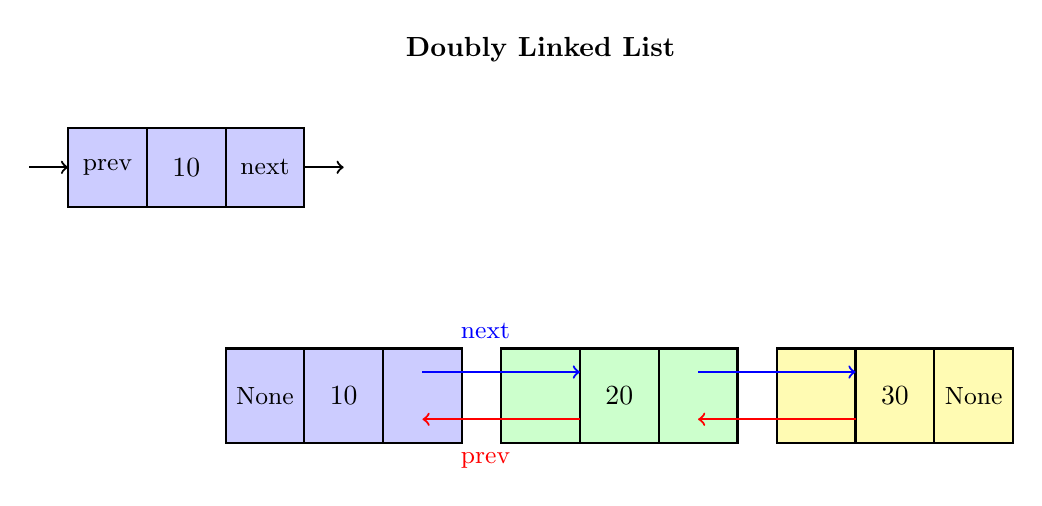
\begin{tikzpicture}[scale=1.0]
    \node at (6, 6) {\textbf{Doubly Linked List}};
        
    % Node structure
    \draw[thick, fill=blue!20] (0,4) rectangle (3,5);
    \draw[thick] (1,4) -- (1,5);
    \draw[thick] (2,4) -- (2,5);
    \node[font=\small] at (0.5, 4.5) {prev};
    \node at (1.5, 4.5) {10};
    \node[font=\small] at (2.5, 4.5) {next};
    \draw[<-, thick] (0, 4.5) -- (-0.5, 4.5);
    \draw[->, thick] (3, 4.5) -- (3.5, 4.5);    
    
    % Full list
    \draw[thick, fill=blue!20] (2,1) rectangle (5,2.2);
    \draw[thick] (3,1) -- (3,2.2);
    \draw[thick] (4,1) -- (4,2.2);
    \node[font=\small] at (2.5, 1.6) {None};
    \node at (3.5, 1.6) {10};
    
    \draw[thick, fill=green!20] (5.5,1) rectangle (8.5,2.2);
    \draw[thick] (6.5,1) -- (6.5,2.2);
    \draw[thick] (7.5,1) -- (7.5,2.2);
    \node at (7, 1.6) {20};
    
    \draw[thick, fill=yellow!30] (9,1) rectangle (12,2.2);
    \draw[thick] (10,1) -- (10,2.2);
    \draw[thick] (11,1) -- (11,2.2);
    \node at (10.5, 1.6) {30};
    \node[font=\small] at (11.5, 1.6) {None};
    
    % Forward arrows (next)
    \draw[->, thick, blue] (4.5, 1.9) -- (6.5, 1.9);
    \draw[->, thick, blue] (8, 1.9) -- (10, 1.9);
    
    % Backward arrows (prev)
    \draw[<-, thick, red] (4.5, 1.3) -- (6.5, 1.3);
    \draw[<-, thick, red] (8, 1.3) -- (10, 1.3);
    
    % Labels
    \node[blue, above, font=\small] at (5.3, 2.2) {next};
    \node[red, below, font=\small] at (5.3, 1.0) {prev};
\end{tikzpicture}
\end{center}

\subsection{Doubly Linked List Implementation}

\begin{lstlisting}
class DNode:
    def __init__(self, data):
        self.data = data
        self.next = None
        self.prev = None  # NEW: pointer to previous

class DoublyLinkedList:
    def __init__(self):
        self.head = None
        self.tail = None  # Keep track of last node too!
        self.size = 0
    
    def prepend(self, data):
        """Insert at beginning - O(1)"""
        new_node = DNode(data)
        
        if self.is_empty():
            self.head = self.tail = new_node
        else:
            new_node.next = self.head
            self.head.prev = new_node
            self.head = new_node
        
        self.size += 1
    
    def append(self, data):
        """Insert at end - O(1) with tail pointer!"""
        new_node = DNode(data)
        
        if self.is_empty():
            self.head = self.tail = new_node
        else:
            new_node.prev = self.tail
            self.tail.next = new_node
            self.tail = new_node
        
        self.size += 1
    
    def delete(self, data):
        """Delete node - easier with prev pointer!"""
        current = self.head
        
        while current is not None:
            if current.data == data:
                # Update previous node
                if current.prev:
                    current.prev.next = current.next
                else:
                    self.head = current.next
                
                # Update next node
                if current.next:
                    current.next.prev = current.prev
                else:
                    self.tail = current.prev
                
                self.size -= 1
                return True
            
            current = current.next
        
        return False
    
    def is_empty(self):
        return self.head is None

# Usage
dll = DoublyLinkedList()
dll.append(10)
dll.append(20)
dll.append(30)
# Can efficiently go both directions!
\end{lstlisting}

\textbf{Advantages:}
\begin{itemize}
    \item Can traverse backwards
    \item Append is $O(1)$ (with tail pointer)
    \item Deletion is easier (don't need to find previous)
\end{itemize}

\textbf{Disadvantage:}
\begin{itemize}
    \item Extra memory for prev pointer
    \item More pointers to update
\end{itemize}

\section{Circular Linked Lists: The Loop}

\subsection{What if the Last Node Points Back to First?}

\begin{center}
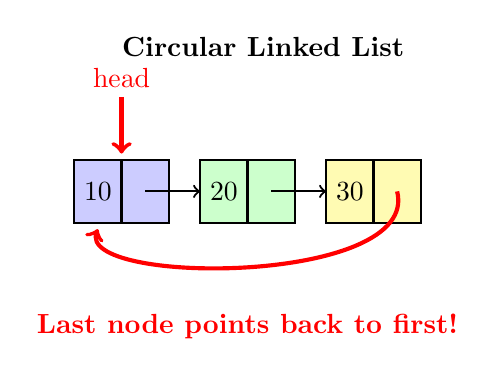
\begin{tikzpicture}[scale=0.8]
    \node at (3, 3.8) {\textbf{Circular Linked List}};
    
    % Nodes
    \draw[thick, fill=blue!20] (0,1) rectangle (1.5,2);
    \draw[thick] (0.75,1) -- (0.75,2);
    \node at (0.375, 1.5) {10};
    \draw[->, thick] (1.125, 1.5) -- (2, 1.5);
    
    \draw[thick, fill=green!20] (2,1) rectangle (3.5,2);
    \draw[thick] (2.75,1) -- (2.75,2);
    \node at (2.375, 1.5) {20};
    \draw[->, thick] (3.125, 1.5) -- (4, 1.5);
    
    \draw[thick, fill=yellow!30] (4,1) rectangle (5.5,2);
    \draw[thick] (4.75,1) -- (4.75,2);
    \node at (4.375, 1.5) {30};
    
    % Circular arrow back to head
    \draw[->, thick, red, line width=1.5pt] (5.125, 1.5) .. controls (5.5, 0) and (0, 0) .. (0.375, 0.9);
    \node[red, below] at (2.75, -0.3) {\textbf{Last node points back to first!}};
    
    \draw[->, ultra thick, red] (0.75, 3) -- (0.75, 2.1);
    \node[red] at (0.75, 3.3) {head};
\end{tikzpicture}
\end{center}

\textbf{Use cases:}
\begin{itemize}
    \item Round-robin scheduling
    \item Music playlists (loop)
    \item Circular buffers
\end{itemize}

\begin{warning}
\textbf{Watch out!} Must be careful with traversal — there's no \texttt{None} to stop at!

\begin{lstlisting}
def traverse_circular(self):
    """Must use different stop condition"""
    if self.is_empty():
        return
    
    current = self.head
    first = True
    
    while first or current != self.head:
        print(current.data)
        current = current.next
        first = False
    # Stop when we circle back to head
\end{lstlisting}
\end{warning}

\section{Common Linked List Patterns and Tricks}

\subsection{Pattern 1: Two Pointers (Slow and Fast)}

\textbf{Problem:} Find the middle element of a linked list in one pass.

\textbf{Solution:} Use two pointers — one moves twice as fast!

\begin{lstlisting}
def find_middle(self):
    """
    Find middle node using slow/fast pointers.
    When fast reaches end, slow is at middle!
    """
    if self.is_empty():
        return None
    
    slow = self.head
    fast = self.head
    
    while fast is not None and fast.next is not None:
        slow = slow.next      # Move 1 step
        fast = fast.next.next # Move 2 steps
    
    return slow  # Slow is at middle!

# Example: 1->2->3->4->5
# When fast is at 5, slow is at 3 (middle)
\end{lstlisting}

\begin{center}
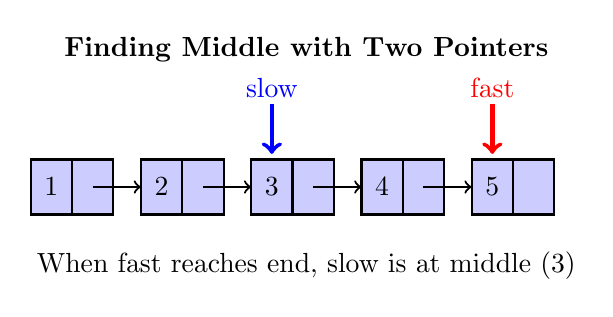
\begin{tikzpicture}[scale=0.7]
    \node at (5, 4.5) {\textbf{Finding Middle with Two Pointers}};
    
    % Nodes
    \foreach \x/\val in {0/1, 2/2, 4/3, 6/4, 8/5} {
        \draw[thick, fill=blue!20] (\x,1.5) rectangle (\x+1.5,2.5);
        \draw[thick] (\x+0.75,1.5) -- (\x+0.75,2.5);
        \node at (\x+0.375, 2) {\val};
        \ifnum\x<8
            \draw[->, thick] (\x+1.125, 2) -- (\x+2, 2);
        \fi
    }
    
    % Slow pointer
    \draw[->, ultra thick, blue] (4.375, 3.5) -- (4.375, 2.6);
    \node[blue] at (4.375, 3.8) {slow};
    
    % Fast pointer
    \draw[->, ultra thick, red] (8.375, 3.5) -- (8.375, 2.6);
    \node[red] at (8.375, 3.8) {fast};
    
    \node[below] at (5, 1) {When fast reaches end, slow is at middle (3)};
\end{tikzpicture}
\end{center}

\textbf{Time:} $O(n)$, \textbf{Space:} $O(1)$ — elegant!

\subsection{Pattern 2: Reverse a Linked List}

\textbf{Problem:} Reverse the entire list.

\begin{lstlisting}
def reverse(self):
    """
    Reverse linked list in-place.
    Key: Reverse the direction of all arrows!
    """
    prev = None
    current = self.head
    
    while current is not None:
        # Save next node
        next_node = current.next
        
        # Reverse the arrow
        current.next = prev
        
        # Move forward
        prev = current
        current = next_node
    
    # Update head
    self.head = prev

# Before: 1->2->3->None
# After:  3->2->1->None
\end{lstlisting}

\begin{center}
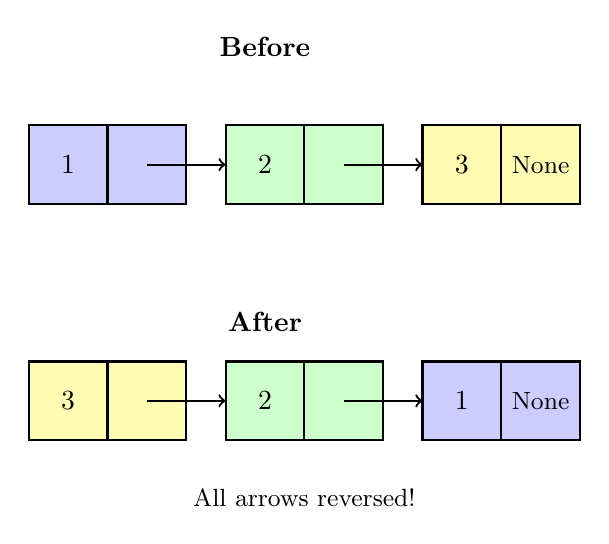
\begin{tikzpicture}[scale=1.0]
    % Before
    \node at (3, 5) {\textbf{Before}};
    
    \draw[thick, fill=blue!20] (0,3) rectangle (2,4);
    \draw[thick] (1,3) -- (1,4);
    \node at (0.5, 3.5) {1};
    \draw[->, thick] (1.5, 3.5) -- (2.5, 3.5);
    
    \draw[thick, fill=green!20] (2.5,3) rectangle (4.5,4);
    \draw[thick] (3.5,3) -- (3.5,4);
    \node at (3, 3.5) {2};
    \draw[->, thick] (4, 3.5) -- (5, 3.5);
    
    \draw[thick, fill=yellow!30] (5,3) rectangle (7,4);
    \draw[thick] (6,3) -- (6,4);
    \node at (5.5, 3.5) {3};
    \node[font=\small] at (6.5, 3.5) {None};
    
    % After
    \node at (3, 1.5) {\textbf{After}};
    
    \draw[thick, fill=yellow!30] (0,0) rectangle (2,1);
    \draw[thick] (1,0) -- (1,1);
    \node at (0.5, 0.5) {3};
    \draw[->, thick] (1.5, 0.5) -- (2.5, 0.5);
    
    \draw[thick, fill=green!20] (2.5,0) rectangle (4.5,1);
    \draw[thick] (3.5,0) -- (3.5,1);
    \node at (3, 0.5) {2};
    \draw[->, thick] (4, 0.5) -- (5, 0.5);
    
    \draw[thick, fill=blue!20] (5,0) rectangle (7,1);
    \draw[thick] (6,0) -- (6,1);
    \node at (5.5, 0.5) {1};
    \node[font=\small] at (6.5, 0.5) {None};
    
    \node[below, font=\small] at (3.5, -0.5) {All arrows reversed!};
\end{tikzpicture}
\end{center}

\subsection{Pattern 3: Detect Cycle (Floyd's Algorithm)}

\textbf{Problem:} Is there a cycle in the linked list?

\textbf{Solution:} Slow and fast pointers again! If there's a cycle, fast will eventually catch slow.

\begin{lstlisting}
def has_cycle(self):
    """
    Detect if list has a cycle using Floyd's algorithm.
    If fast catches slow, there's a cycle!
    """
    if self.is_empty():
        return False
    
    slow = self.head
    fast = self.head
    
    while fast is not None and fast.next is not None:
        slow = slow.next
        fast = fast.next.next
        
        if slow == fast:  # They met!
            return True
    
    return False  # Fast reached end, no cycle

# Think of it like a race track:
# If it's circular, the faster runner will lap the slower one!
\end{lstlisting}

\begin{center}
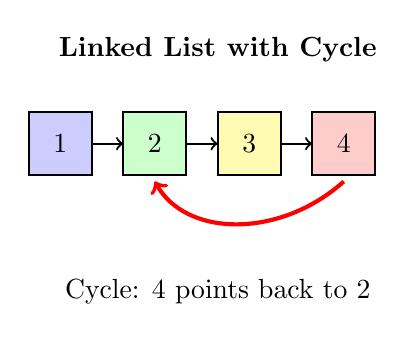
\begin{tikzpicture}[scale=0.8]
    \node at (3, 3) {\textbf{Linked List with Cycle}};
    
    % Nodes
    \draw[thick, fill=blue!20] (0,1) rectangle (1,2);
    \node at (0.5, 1.5) {1};
    \draw[->, thick] (1, 1.5) -- (1.5, 1.5);
    
    \draw[thick, fill=green!20] (1.5,1) rectangle (2.5,2);
    \node at (2, 1.5) {2};
    \draw[->, thick] (2.5, 1.5) -- (3, 1.5);
    
    \draw[thick, fill=yellow!30] (3,1) rectangle (4,2);
    \node at (3.5, 1.5) {3};
    \draw[->, thick] (4, 1.5) -- (4.5, 1.5);
    
    \draw[thick, fill=red!20] (4.5,1) rectangle (5.5,2);
    \node at (5, 1.5) {4};
    
    % Cycle back
    \draw[->, thick, red, line width=1.5pt] (5, 0.9) .. controls (4, 0) and (2.5, 0) .. (2, 0.9);
    
    \node[below] at (3, -0.5) {Cycle: 4 points back to 2};
\end{tikzpicture}
\end{center}

\section{Practice Problems}

\subsection{Problem 1: Remove Duplicates from Sorted List}

\begin{lstlisting}
def remove_duplicates_sorted(self):
    """
    Remove duplicates from sorted linked list.
    Example: 1->1->2->3->3 becomes 1->2->3
    """
    if self.is_empty():
        return
    
    current = self.head
    
    while current is not None and current.next is not None:
        if current.data == current.next.data:
            # Skip duplicate
            current.next = current.next.next
            self.size -= 1
        else:
            # Move forward
            current = current.next

# Time: O(n), Space: O(1)
\end{lstlisting}

\subsection{Problem 2: Merge Two Sorted Lists}

\begin{lstlisting}
def merge_sorted_lists(list1, list2):
    """
    Merge two sorted linked lists into one sorted list.
    Example: 
        1->3->5 and 2->4->6 
        becomes 1->2->3->4->5->6
    """
    # Create dummy head for easier handling
    dummy = Node(0)
    current = dummy
    
    p1 = list1.head
    p2 = list2.head
    
    while p1 is not None and p2 is not None:
        if p1.data <= p2.data:
            current.next = p1
            p1 = p1.next
        else:
            current.next = p2
            p2 = p2.next
        current = current.next
    
    # Attach remaining nodes
    if p1 is not None:
        current.next = p1
    if p2 is not None:
        current.next = p2
    
    # Create result list
    result = LinkedList()
    result.head = dummy.next
    return result

# Time: O(n + m), Space: O(1)
\end{lstlisting}

\subsection{Problem 3: Check if Palindrome}

\begin{lstlisting}
def is_palindrome(self):
    """
    Check if linked list is palindrome.
    Example: 1->2->3->2->1 is palindrome
    """
    if self.is_empty() or self.head.next is None:
        return True
    
    # Step 1: Find middle using slow/fast
    slow = fast = self.head
    while fast and fast.next:
        slow = slow.next
        fast = fast.next.next
    
    # Step 2: Reverse second half
    prev = None
    current = slow
    while current:
        next_node = current.next
        current.next = prev
        prev = current
        current = next_node
    
    # Step 3: Compare first half with reversed second half
    left = self.head
    right = prev
    
    while right:  # Compare until second half ends
        if left.data != right.data:
            return False
        left = left.next
        right = right.next
    
    return True

# Time: O(n), Space: O(1) - clever!
\end{lstlisting}

\subsection{Problem 4: Find Nth Node from End}

\begin{lstlisting}
def nth_from_end(self, n):
    """
    Find nth node from end in one pass.
    Example: 1->2->3->4->5, n=2 returns 4
    
    Trick: Use two pointers, n nodes apart!
    """
    if self.is_empty():
        return None
    
    # Move first pointer n steps ahead
    first = self.head
    for _ in range(n):
        if first is None:
            return None  # n is larger than list size
        first = first.next
    
    # Move both pointers together
    second = self.head
    while first is not None:
        first = first.next
        second = second.next
    
    return second

# When first reaches end, second is n from end!
# Time: O(n), Space: O(1)
\end{lstlisting}

\section{When to Use Linked Lists}

\begin{center}
\begin{tabular}{|p{6cm}|p{6cm}|}
\hline
\textbf{Use Linked List When:} & \textbf{Use Array When:} \\
\hline
Frequent insertions/deletions & Need random access by index \\
Don't know size in advance & Size is fixed or predictable \\
Don't need random access & Need cache-friendly memory \\
Implementing stack/queue & Need to search frequently \\
Building complex structures (graphs) & Working with small data \\
\hline
\end{tabular}
\end{center}

\section{Key Takeaways}

\begin{enumerate}
    \item \textbf{Linked lists = Scattered memory} connected by pointers
    
    \item \textbf{Node = Data + Pointer(s)} to next (and prev in doubly)
    
    \item \textbf{Tradeoff:} 
    \begin{itemize}
        \item Good: $O(1)$ insert/delete at known position
        \item Bad: $O(n)$ access by index, $O(n)$ search
    \end{itemize}
    
    \item \textbf{Variants:}
    \begin{itemize}
        \item Singly: One direction only
        \item Doubly: Bidirectional, easier deletion
        \item Circular: Last connects to first
    \end{itemize}
    
    \item \textbf{Two-pointer technique:} Powerful for many problems
    \begin{itemize}
        \item Find middle (slow/fast)
        \item Detect cycle (Floyd's)
        \item Nth from end (gap of n)
    \end{itemize}
    
    \item \textbf{Always consider:} What are you doing most frequently?
\end{enumerate}

\begin{insight}
Gilbert Strang's wisdom: "Arrays and linked lists are the yin and yang of data structures. Arrays give you speed of access through contiguous memory. Linked lists give you flexibility of modification through pointers. Neither is 'better' — they're different tools for different jobs. Master both, understand their tradeoffs, and you'll always choose wisely."
\end{insight}

\section{Looking Ahead to Chapter 6}

We've seen linear structures: arrays, stacks, queues, linked lists. But what if we need \textbf{instant lookups} by key, like a real dictionary?

Enter \textbf{Hash Tables} — one of the most powerful data structures in computer science. They give us $O(1)$ average-case search, insert, and delete. How? Through the magic of hashing!

Get ready to understand how Python dictionaries actually work under the hood!

\vspace{1cm}

\begin{center}
\rule{0.5\textwidth}{0.4pt}

\textit{"Pointers are not scary. They're just addresses. And addresses lead you to treasure."}

\rule{0.5\textwidth}{0.4pt}
\end{center}
\pagebreak
\section{Chapter 6: Hash Tables and Dictionaries}
\subsection*{The Magic of Instant Lookup}

\begin{center}
\textit{"A hash table is like a library where books magically jump to your hand when you call their name."}
\end{center}

\section{The Big Picture: The Search Problem}

Imagine you have a phone book with 1 million names. How do you find "Smith, John"?

\textbf{Option 1 (Array):} Check every entry from start → $O(n)$ = 1 million checks!

\textbf{Option 2 (Sorted Array + Binary Search):} Jump to middle, narrow down → $O(\log n)$ = 20 checks

\textbf{Option 3 (Hash Table):} Compute "Smith, John" → magical index → Done! → $O(1)$ = 1 check!

\begin{keyidea}
\textbf{The Dream:} Given any key (like a name), instantly compute where the value should be stored.

This is the promise of hash tables: \textbf{constant-time lookup, insert, and delete} (on average).
\end{keyidea}

\section{First Principles: How Hash Tables Work}

\subsection{The Core Idea: Direct Addressing}

Imagine if we could use the data itself as an array index:

\begin{center}
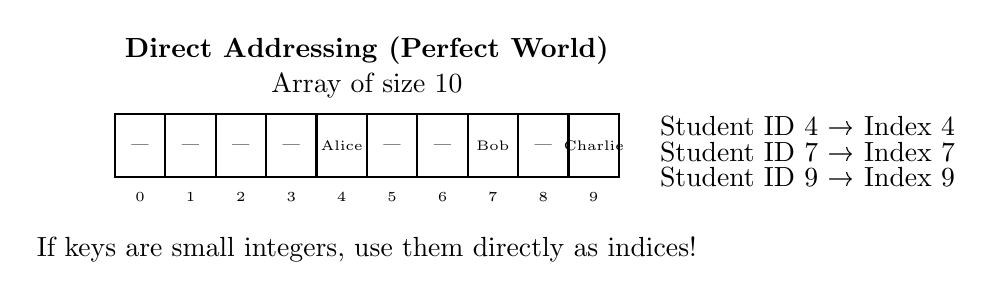
\begin{tikzpicture}[scale=0.8]
    \node at (4, 4) {\textbf{Direct Addressing (Perfect World)}};
    
    % Array
    \foreach \x/\val in {0/—, 1/—, 2/—, 3/—, 4/Alice, 5/—, 6/—, 7/Bob, 8/—, 9/Charlie} {
        \draw[thick] (\x*0.8, 2) rectangle (\x*0.8+0.8, 3);
        \node[font=\tiny] at (\x*0.8+0.4, 2.5) {\val};
        \node[below, font=\tiny] at (\x*0.8+0.4, 1.9) {\x};
    }
    
    \node[above] at (4, 3.1) {Array of size 10};
    
    % Examples
    \node[right] at (8.5, 2.8) {Student ID 4 → Index 4};
    \node[right] at (8.5, 2.4) {Student ID 7 → Index 7};
    \node[right] at (8.5, 2.0) {Student ID 9 → Index 9};
    
    \node[below] at (4, 1.2) {If keys are small integers, use them directly as indices!};
\end{tikzpicture}
\end{center}

\textbf{Problem:} What if keys aren't small integers? What if we have:
\begin{itemize}
    \item Strings: "Alice", "Bob"
    \item Large numbers: 9876543210
    \item Complex objects
\end{itemize}

\textbf{Solution:} Use a \textbf{hash function} to convert ANY key into a valid array index!

\subsection{The Hash Function: The Magic Converter}

\begin{center}
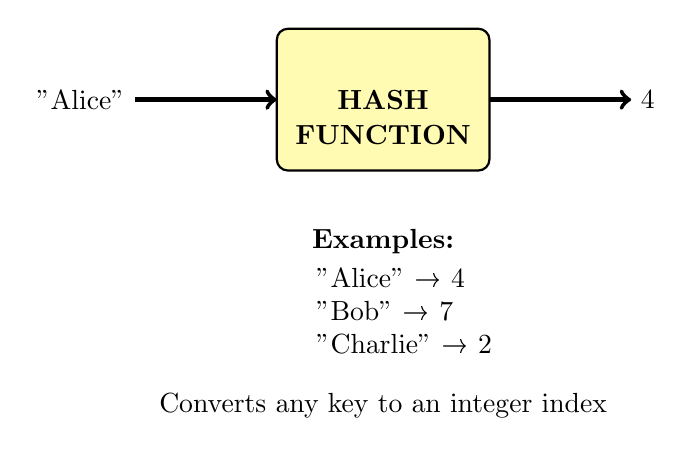
\begin{tikzpicture}[scale=0.9]
    % Hash function box
    \draw[thick, fill=yellow!30, rounded corners] (2, 2) rectangle (5, 4);
    \node at (3.5, 3) {\textbf{HASH}};
    \node at (3.5, 2.5) {\textbf{FUNCTION}};
    
    % Input
    \draw[->, ultra thick] (0, 3) -- (2, 3);
    \node[left] at (0, 3) {"Alice"};
    
    % Output
    \draw[->, ultra thick] (5, 3) -- (7, 3);
    \node[right] at (7, 3) {4};
    
    % Examples
    \node at (3.5, 1) {\textbf{Examples:}};
    \node[align=left] at (3.8, 0.02) {
        "Alice" → 4 \\
        "Bob" → 7 \\
        "Charlie" → 2
    };
    
    \node[below] at (3.5, -1) {Converts any key to an integer index};
\end{tikzpicture}
\end{center}

\begin{keyidea}
A \textbf{hash function} $h(key)$ takes any key and returns an integer (the hash code):

\[
h(\text{key}) \to \text{integer from 0 to table\_size - 1}
\]

\textbf{Requirements:}
\begin{enumerate}
    \item \textbf{Deterministic:} Same key always gives same hash
    \item \textbf{Fast:} Should compute in $O(1)$
    \item \textbf{Uniform:} Spread keys evenly across indices
\end{enumerate}
\end{keyidea}

\section{Building a Hash Function: From Scratch}

\subsection{Example 1: Simple String Hash}

Let's hash strings by summing ASCII values:

\begin{lstlisting}
def simple_hash(key, table_size):
    """
    Hash a string by summing character values.
    Example: "cat" = ord('c') + ord('a') + ord('t')
                    = 99 + 97 + 116 = 312
    """
    hash_value = 0
    for char in key:
        hash_value += ord(char)  # ASCII value
    
    # Ensure index fits in table
    return hash_value % table_size

# Test
table_size = 10
print(simple_hash("cat", table_size))    # Some index 0-9
print(simple_hash("dog", table_size))    # Different index
print(simple_hash("act", table_size))    # Same as "cat"! (collision)
\end{lstlisting}

\textbf{Problem:} "cat" and "act" have same hash (anagrams)! This is a \textbf{collision}.

\subsection{Example 2: Better Hash (Polynomial Rolling)}

Consider position of characters:

\begin{lstlisting}
def better_hash(key, table_size):
    """
    Polynomial hash: each position matters.
    hash = s[0]*31^(n-1) + s[1]*31^(n-2) + ... + s[n-1]
    """
    hash_value = 0
    for char in key:
        hash_value = hash_value * 31 + ord(char)
    
    return hash_value % table_size

# Now "cat" and "act" give different hashes!
print(better_hash("cat", 10))  # Different
print(better_hash("act", 10))  # from this
\end{lstlisting}

\textbf{Why 31?} It's a prime number that works well in practice. Primes help distribute values evenly.

\subsection{Python's Built-in Hash}

Python has a built-in \texttt{hash()} function:

\begin{lstlisting}
print(hash("Alice"))     # Some large integer
print(hash("Bob"))       # Different integer
print(hash(42))          # Works on numbers too
print(hash((1, 2, 3)))   # And tuples

# To fit in table:
table_size = 10
index = hash("Alice") % table_size
\end{lstlisting}

\section{The Collision Problem}

\subsection{What Are Collisions?}

Even with good hash functions, different keys can hash to the same index:

\begin{center}
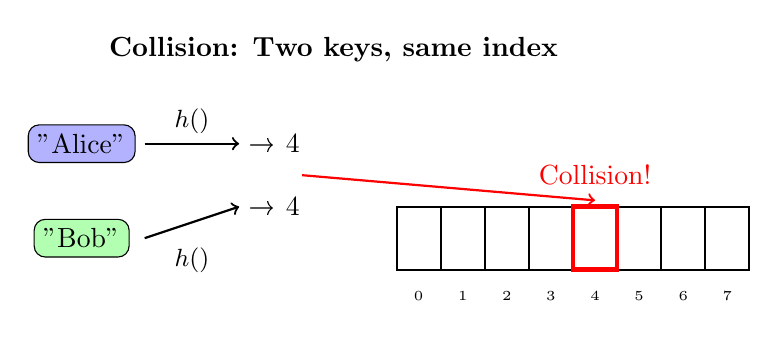
\begin{tikzpicture}[scale=0.8]
    \node at (5, 4) {\textbf{Collision: Two keys, same index}};
    
    % Keys
    \node[fill=blue!30, draw, rounded corners] at (1, 2.5) {"Alice"};
    \node[fill=green!30, draw, rounded corners] at (1, 1) {"Bob"};
    
    % Hash arrows
    \draw[->, thick] (2, 2.5) -- (3.5, 2.5);
    \node[above] at (2.75, 2.5) {\small $h()$};
    \draw[->, thick] (2, 1) -- (3.5, 1.5);
    \node[below] at (2.75, 1) {\small $h()$};
    
    % Both point to index 4
    \node[right] at (3.5, 2.5) {→ 4};
    \node[right] at (3.5, 1.5) {→ 4};
    
    % Array
    \foreach \x in {0,...,7} {
        \draw[thick] (6+\x*0.7, 0.5) rectangle (6+\x*0.7+0.7, 1.5);
        \node[below, font=\tiny] at (6+\x*0.7+0.35, 0.3) {\x};
    }
    
    % Highlight collision spot
    \draw[ultra thick, red] (6+4*0.7, 0.5) rectangle (6+4*0.7+0.7, 1.5);
    \node[red, above] at (6+4*0.7+0.35, 1.7) {Collision!};
    
    \draw[->, thick, red] (4.5, 2) -- (6+4*0.7+0.35, 1.6);
\end{tikzpicture}
\end{center}

\begin{insight}
\textbf{Birthday Paradox:} With only 23 people, there's >50\% chance two share a birthday!

Similarly, with a hash table of size 365, you'll likely get collisions with just 23 keys. Collisions are \textbf{inevitable} — we must handle them!
\end{insight}

\subsection{Solution 1: Chaining (Linked Lists)}

Each array slot stores a \textbf{linked list} of all items that hash there:

\begin{center}
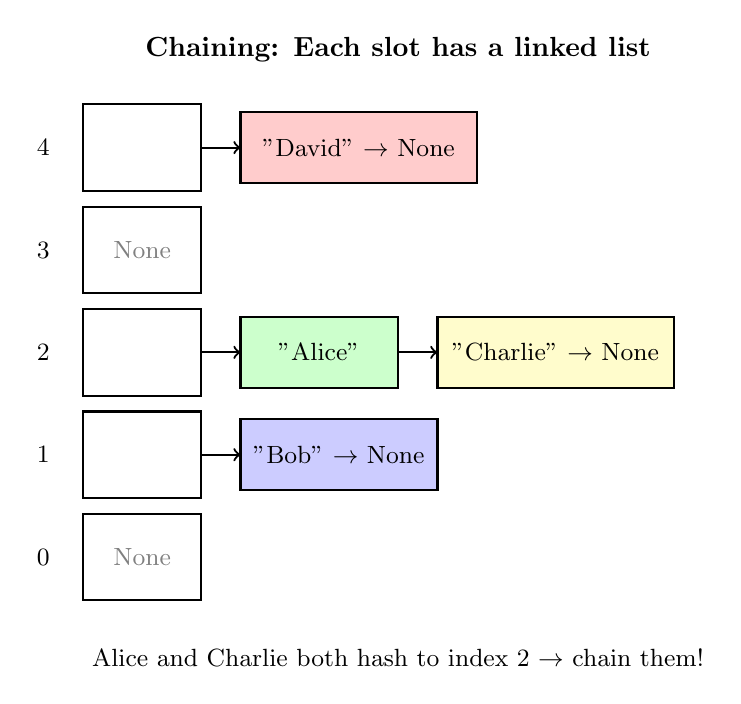
\begin{tikzpicture}[scale=1.0]
    \node at (4, 7) {\textbf{Chaining: Each slot has a linked list}};
    
    % Hash table array
    \foreach \x in {0,...,4} {
        \draw[thick] (0, \x*1.3) rectangle (1.5, \x*1.3+1.1);
        \node[left, font=\small] at (-0.3, \x*1.3+0.55) {\x};
    }
    
    % Slot 0: empty
    \node[gray, font=\small] at (0.75, 0.55) {None};
    
    % Slot 1: one item
    \draw[->, thick] (1.5, 1.85) -- (2, 1.85);
    \draw[thick, fill=blue!20] (2, 1.4) rectangle (4.5, 2.3);
    \node[font=\small] at (3.25, 1.85) {"Bob" $\to$ None};
    
    % Slot 2: two items (chain!)
    \draw[->, thick] (1.5, 3.15) -- (2, 3.15);
    \draw[thick, fill=green!20] (2, 2.7) rectangle (4, 3.6);
    \node[font=\small] at (3, 3.15) {"Alice"};
    \draw[->, thick] (4, 3.15) -- (4.5, 3.15);
    \draw[thick, fill=yellow!20] (4.5, 2.7) rectangle (7.5, 3.6);
    \node[font=\small] at (6, 3.15) {"Charlie" $\to$ None};
    
    % Slot 3: empty
    \node[gray, font=\small] at (0.75, 4.45) {None};
    
    % Slot 4: one item
    \draw[->, thick] (1.5, 5.75) -- (2, 5.75);
    \draw[thick, fill=red!20] (2, 5.3) rectangle (5, 6.2);
    \node[font=\small] at (3.5, 5.75) {"David" $\to$ None};
    
    \node[below, font=\small] at (4, -0.5) {Alice and Charlie both hash to index 2 $\to$ chain them!};
\end{tikzpicture}
\end{center}

\textbf{How it works:}
\begin{itemize}
    \item Compute $\text{index} = h(\text{key})$
    \item Go to \texttt{table[index]}
    \item Search through linked list for the key
    \item If found, update/return value
    \item If not found, append to list
\end{itemize}

\textbf{Performance:}
\begin{itemize}
    \item \textbf{Best case:} $O(1)$ — no collisions
    \item \textbf{Worst case:} $O(n)$ — all keys hash to same index!
    \item \textbf{Average case:} $O(1 + \alpha)$ where $\alpha = n/m$ (load factor)
\end{itemize}

\subsection{Solution 2: Open Addressing (Linear Probing)}

If a slot is occupied, try the next one:

\begin{center}
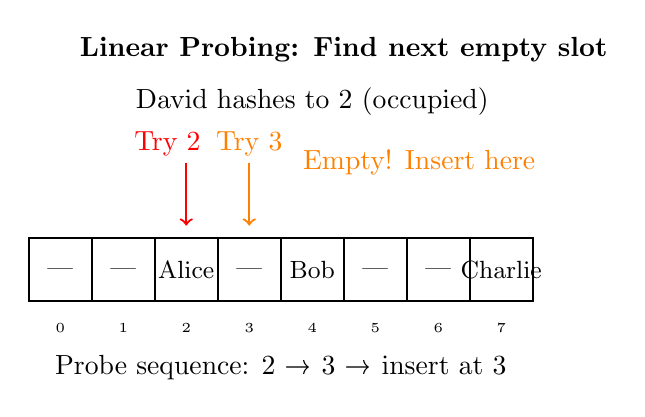
\begin{tikzpicture}[scale=0.8]
    \node at (5, 6) {\textbf{Linear Probing: Find next empty slot}};
    
    % Array
    \foreach \x/\val in {0/—, 1/—, 2/Alice, 3/—, 4/Bob, 5/—, 6/—, 7/Charlie} {
        \draw[thick] (\x, 2) rectangle (\x+1, 3);
        \node[font=\small] at (\x+0.5, 2.5) {\val};
        \node[below, font=\tiny] at (\x+0.5, 1.8) {\x};
    }
    
    % Show probing
    \node[above] at (4.5, 4.8) {David hashes to 2 (occupied)};
    \draw[->, thick, red] (2.5, 4.2) -- (2.5, 3.2);
    \node[red] at (2.2, 4.5) {Try 2};
    \draw[->, thick, orange] (3.5, 4.2) -- (3.5, 3.2);
    \node[orange] at (3.5, 4.5) {Try 3};
    \node[orange, right] at (4.2, 4.2) {Empty! Insert here};
    
    \node[below] at (4, 1.3) {Probe sequence: 2 → 3 → insert at 3};
\end{tikzpicture}
\end{center}

\textbf{Probing strategies:}
\begin{itemize}
    \item \textbf{Linear:} Try index, index+1, index+2, ...
    \item \textbf{Quadratic:} Try index, index+$1^2$, index+$2^2$, index+$3^2$, ...
    \item \textbf{Double hashing:} Use second hash function for step size
\end{itemize}

\textbf{Problem:} \textbf{Clustering} — filled slots create traffic jams

\section{Implementing a Hash Table with Chaining}

\begin{lstlisting}
class HashTable:
    def __init__(self, size=10):
        self.size = size
        self.table = [[] for _ in range(size)]  # List of lists (chains)
        self.count = 0
    
    def _hash(self, key):
        """Hash function using Python's built-in hash"""
        return hash(key) % self.size
    
    def put(self, key, value):
        """Insert or update key-value pair - O(1) average"""
        index = self._hash(key)
        
        # Check if key already exists (update)
        for i, (k, v) in enumerate(self.table[index]):
            if k == key:
                self.table[index][i] = (key, value)
                return
        
        # Key doesn't exist, append to chain
        self.table[index].append((key, value))
        self.count += 1
    
    def get(self, key):
        """Retrieve value by key - O(1) average"""
        index = self._hash(key)
        
        # Search through chain
        for k, v in self.table[index]:
            if k == key:
                return v
        
        raise KeyError(f"Key '{key}' not found")
    
    def delete(self, key):
        """Remove key-value pair - O(1) average"""
        index = self._hash(key)
        
        # Search and remove from chain
        for i, (k, v) in enumerate(self.table[index]):
            if k == key:
                self.table[index].pop(i)
                self.count -= 1
                return v
        
        raise KeyError(f"Key '{key}' not found")
    
    def __contains__(self, key):
        """Check if key exists (for 'in' operator)"""
        try:
            self.get(key)
            return True
        except KeyError:
            return False
    
    def load_factor(self):
        """Return load factor (average chain length)"""
        return self.count / self.size
    
    def __str__(self):
        """String representation"""
        result = []
        for i, chain in enumerate(self.table):
            if chain:
                result.append(f"  {i}: {chain}")
        return "HashTable:\n" + "\n".join(result)

# Usage
ht = HashTable(size=5)
ht.put("Alice", 25)
ht.put("Bob", 30)
ht.put("Charlie", 35)
ht.put("David", 28)

print(ht.get("Alice"))    # 25
print("Bob" in ht)        # True
ht.put("Alice", 26)       # Update
print(ht.get("Alice"))    # 26

print(ht)
print(f"Load factor: {ht.load_factor():.2f}")
\end{lstlisting}

\section{Load Factor and Resizing}

\subsection{What is Load Factor?}

\[
\alpha = \frac{n}{m} = \frac{\text{number of items}}{\text{table size}}
\]

\begin{center}
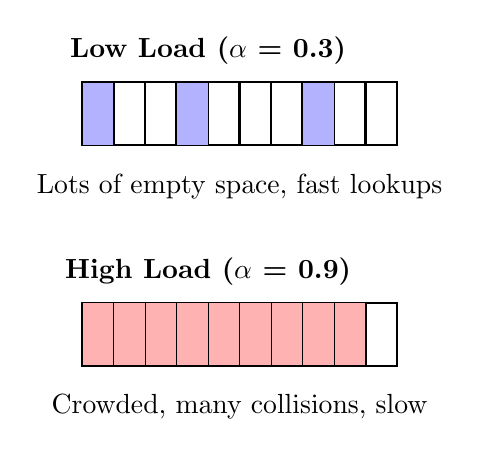
\begin{tikzpicture}[scale=0.8]
    % Low load factor
    \node at (2, 4) {\textbf{Low Load ($\alpha$ = 0.3)}};
    \foreach \x in {0,...,9} {
        \draw[thick] (\x*0.5, 2.5) rectangle (\x*0.5+0.5, 3.5);
    }
    \draw[fill=blue!30] (0, 2.5) rectangle (0.5, 3.5);
    \draw[fill=blue!30] (1.5, 2.5) rectangle (2, 3.5);
    \draw[fill=blue!30] (3.5, 2.5) rectangle (4, 3.5);
    \node[below] at (2.5, 2.2) {Lots of empty space, fast lookups};
    
    % High load factor
    \node at (2, 0.5) {\textbf{High Load ($\alpha$ = 0.9)}};
    \foreach \x in {0,...,9} {
        \draw[thick] (\x*0.5, -1) rectangle (\x*0.5+0.5, 0);
    }
    \foreach \x in {0,1,2,3,4,5,6,7,8} {
        \draw[fill=red!30] (\x*0.5, -1) rectangle (\x*0.5+0.5, 0);
    }
    \node[below] at (2.5, -1.3) {Crowded, many collisions, slow};
\end{tikzpicture}
\end{center}

\begin{keyidea}
\textbf{Rule of Thumb:} Keep load factor below 0.75

When $\alpha > 0.75$:
\begin{enumerate}
    \item Create new table (usually double the size)
    \item Rehash all existing items into new table
    \item Switch to new table
\end{enumerate}

This is \textbf{dynamic resizing}, just like dynamic arrays!
\end{keyidea}

\subsection{Implementing Resize}

\begin{lstlisting}
def _resize(self):
    """
    Double table size and rehash all items.
    Called when load factor exceeds threshold.
    """
    old_table = self.table
    self.size *= 2
    self.table = [[] for _ in range(self.size)]
    self.count = 0
    
    # Rehash all items
    for chain in old_table:
        for key, value in chain:
            self.put(key, value)  # Will use new hash function

def put(self, key, value):
    """Modified to check load factor"""
    # Check if resize needed
    if self.load_factor() > 0.75:
        self._resize()
    
    # ... rest of put logic ...
\end{lstlisting}

\textbf{Cost of resizing:} $O(n)$ to rehash all items, but happens rarely (like dynamic arrays).

\section{Hash Tables in Python: The dict}

Python's \texttt{dict} is a hash table!

\begin{lstlisting}
# Creating dictionaries
phone_book = {
    "Alice": "555-1234",
    "Bob": "555-5678",
    "Charlie": "555-9012"
}

# Or start empty
grades = {}

# Insert/Update - O(1) average
grades["Alice"] = 95
grades["Bob"] = 87

# Lookup - O(1) average
print(grades["Alice"])  # 95

# Check existence - O(1) average
if "Charlie" in grades:
    print("Charlie has a grade")

# Delete - O(1) average
del grades["Bob"]

# Get with default
score = grades.get("David", 0)  # Returns 0 if not found

# Iterate through keys
for name in phone_book:
    print(name, phone_book[name])

# Iterate through key-value pairs
for name, number in phone_book.items():
    print(f"{name}: {number}")
\end{lstlisting}

\section{Hash Table Applications: Real World}

\subsection{Application 1: Counting Frequencies}

\begin{lstlisting}
def count_words(text):
    """
    Count frequency of each word.
    Example: "hello world hello" -> {"hello": 2, "world": 1}
    """
    word_count = {}
    
    for word in text.split():
        word = word.lower()
        if word in word_count:
            word_count[word] += 1
        else:
            word_count[word] = 1
    
    return word_count

# Or more elegantly:
from collections import defaultdict

def count_words_v2(text):
    word_count = defaultdict(int)  # Default value is 0
    for word in text.split():
        word_count[word.lower()] += 1
    return dict(word_count)

# Even simpler:
from collections import Counter

def count_words_v3(text):
    return Counter(text.lower().split())

text = "hello world hello python world"
print(count_words(text))
# {'hello': 2, 'world': 2, 'python': 1}
\end{lstlisting}

\subsection{Application 2: Two Sum Problem}

\textbf{Problem:} Given array and target, find two numbers that sum to target.

\begin{lstlisting}
def two_sum(nums, target):
    """
    Find indices of two numbers that sum to target.
    
    Brute force: O(n^2) - check all pairs
    Hash table: O(n) - brilliant!
    
    Example: [2, 7, 11, 15], target=9 -> [0, 1]
    """
    seen = {}  # Maps number -> its index
    
    for i, num in enumerate(nums):
        complement = target - num
        
        if complement in seen:
            # Found it! Return indices
            return [seen[complement], i]
        
        # Remember this number
        seen[num] = i
    
    return None  # No solution

# Test
nums = [2, 7, 11, 15]
print(two_sum(nums, 9))   # [0, 1] (2 + 7 = 9)
print(two_sum(nums, 17))  # [0, 2] (2 + 15 = 17)
\end{lstlisting}
\begin{center}
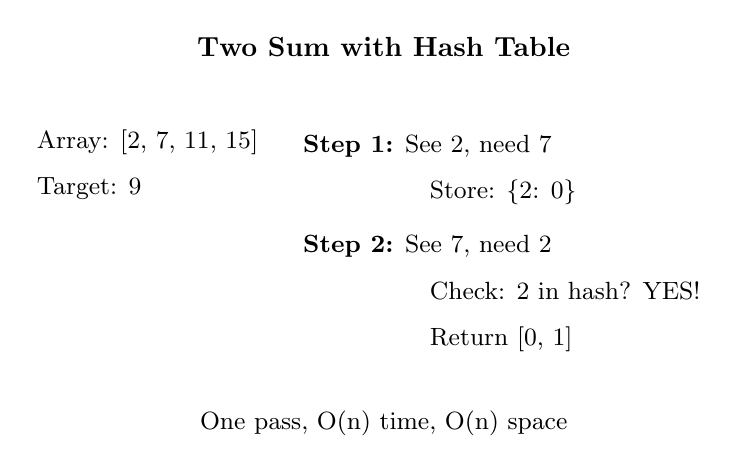
\begin{tikzpicture}[scale=1.0]
    \node at (5, 6) {\textbf{Two Sum with Hash Table}};
    
    \node[align=left, font=\small] at (2, 4.5) {
        Array: [2, 7, 11, 15] \\[0.2cm]
        Target: 9
    };
    
    \node[align=left, font=\small] at (6.5, 3.5) {
        \textbf{Step 1:} See 2, need 7 \\[0.2cm]
        \hspace{1.5cm} Store: \{2: 0\} \\[0.3cm]
        \textbf{Step 2:} See 7, need 2 \\[0.2cm]
        \hspace{1.5cm} Check: 2 in hash? YES! \\[0.2cm]
        \hspace{1.5cm} Return [0, 1]
    };
    
    \node[below, font=\small] at (5, 1.5) {One pass, O(n) time, O(n) space};
\end{tikzpicture}
\end{center}

\subsection{Application 3: Caching/Memoization}

\begin{lstlisting}
def fibonacci_memo(n, cache={}):
    """
    Fibonacci with memoization using hash table.
    Without cache: O(2^n)
    With cache: O(n)
    """
    if n in cache:
        return cache[n]
    
    if n <= 1:
        return n
    
    cache[n] = fibonacci_memo(n-1, cache) + fibonacci_memo(n-2, cache)
    return cache[n]

print(fibonacci_memo(100))  # Instant! Would hang without cache
\end{lstlisting}

\subsection{Application 4: Anagram Detection}

\begin{lstlisting}
def are_anagrams(s1, s2):
    """
    Check if two strings are anagrams.
    Example: "listen" and "silent" are anagrams
    """
    if len(s1) != len(s2):
        return False
    
    # Count character frequencies
    char_count = {}
    
    for char in s1:
        char_count[char] = char_count.get(char, 0) + 1
    
    for char in s2:
        if char not in char_count:
            return False
        char_count[char] -= 1
        if char_count[char] < 0:
            return False
    
    return True

# Or simpler:
from collections import Counter

def are_anagrams_v2(s1, s2):
    return Counter(s1) == Counter(s2)

print(are_anagrams("listen", "silent"))  # True
print(are_anagrams("hello", "world"))    # False
\end{lstlisting}

\section{Sets: Hash Tables Without Values}

A \textbf{set} is a hash table that only stores keys (no values):

\begin{lstlisting}
# Creating sets
fruits = {"apple", "banana", "orange"}
numbers = set([1, 2, 3, 2, 1])  # Duplicates removed: {1, 2, 3}

# Add - O(1)
fruits.add("grape")

# Remove - O(1)
fruits.remove("banana")

# Check membership - O(1)
if "apple" in fruits:
    print("We have apples!")

# Set operations
set1 = {1, 2, 3, 4}
set2 = {3, 4, 5, 6}

print(set1 & set2)  # Intersection: {3, 4}
print(set1 | set2)  # Union: {1, 2, 3, 4, 5, 6}
print(set1 - set2)  # Difference: {1, 2}

# Remove duplicates from list
numbers = [1, 2, 2, 3, 3, 3, 4]
unique = list(set(numbers))  # [1, 2, 3, 4]
\end{lstlisting}

\section{Practice Problems}

\subsection{Problem 1: First Non-Repeating Character}

\begin{lstlisting}
def first_non_repeating(s):
    """
    Find first character that appears only once.
    Example: "leetcode" -> "l"
             "loveleetcode" -> "v"
    """
    # Count frequencies
    char_count = {}
    for char in s:
        char_count[char] = char_count.get(char, 0) + 1
    
    # Find first with count 1
    for char in s:
        if char_count[char] == 1:
            return char
    
    return None

print(first_non_repeating("leetcode"))      # 'l'
print(first_non_repeating("loveleetcode"))  # 'v'
\end{lstlisting}

\subsection{Problem 2: Group Anagrams}

\begin{lstlisting}
def group_anagrams(words):
    """
    Group words that are anagrams.
    Example: ["eat", "tea", "tan", "ate", "nat", "bat"]
    -> [["eat","tea","ate"], ["tan","nat"], ["bat"]]
    """
    anagram_groups = {}
    
    for word in words:
        # Sort word to get canonical form
        key = ''.join(sorted(word))
        
        if key not in anagram_groups:
            anagram_groups[key] = []
        
        anagram_groups[key].append(word)
    
    return list(anagram_groups.values())

words = ["eat", "tea", "tan", "ate", "nat", "bat"]
print(group_anagrams(words))
# [['eat', 'tea', 'ate'], ['tan', 'nat'], ['bat']]
\end{lstlisting}

\subsection{Problem 3: Longest Consecutive Sequence}

\begin{lstlisting}
def longest_consecutive(nums):
    """
    Find length of longest consecutive sequence.
    Example: [100, 4, 200, 1, 3, 2] -> 4
    (sequence is 1, 2, 3, 4)
    
    Brute force: O(n log n) sort
    Hash table: O(n) brilliant solution!
    """
    if not nums:
        return 0
    
    num_set = set(nums)  # For O(1) lookup
    max_length = 0
    
    for num in num_set:
        # Only start counting if this is start of sequence
        if num - 1 not in num_set:
            current = num
            length = 1
            
            # Count consecutive numbers
            while current + 1 in num_set:
                current += 1
                length += 1
            
            max_length = max(max_length, length)
    
    return max_length

nums = [100, 4, 200, 1, 3, 2]
print(longest_consecutive(nums))  # 4 (sequence: 1,2,3,4)
\end{lstlisting}

\subsection{Problem 4: Subarray Sum Equals K}

\begin{lstlisting}
def subarray_sum(nums, k):
    """
    Count subarrays with sum equal to k.
    Example: [1, 1, 1], k=2 -> 2 subarrays: [1,1] and [1,1]
    
    Key insight: Use cumulative sum + hash table
    If cum_sum[j] - cum_sum[i] = k, then subarray i+1..j has sum k
    """
    count = 0
    cum_sum = 0
    sum_count = {0: 1}  # Base case: empty subarray
    
    for num in nums:
        cum_sum += num
        
        # Check if (cum_sum - k) exists
        if cum_sum - k in sum_count:
            count += sum_count[cum_sum - k]
        
        # Update sum count
        sum_count[cum_sum] = sum_count.get(cum_sum, 0) + 1
    
    return count

print(subarray_sum([1, 1, 1], 2))     # 2
print(subarray_sum([1, 2, 3], 3))     # 2
\end{lstlisting}

\section{Hash Function Design: Deep Dive}

\subsection{Properties of Good Hash Functions}

\begin{enumerate}
    \item \textbf{Deterministic:} Same input always produces same output
    \item \textbf{Uniform distribution:} Keys spread evenly across table
    \item \textbf{Fast to compute:} $O(1)$ time
    \item \textbf{Minimize collisions:} Different keys should hash differently
\end{enumerate}

\subsection{Common Hash Function Techniques}

\begin{lstlisting}
# 1. Division method
def hash_division(key, m):
    """Simple: key % m"""
    return key % m

# 2. Multiplication method
def hash_multiplication(key, m):
    """Knuth's method: use golden ratio"""
    A = 0.6180339887  # (sqrt(5) - 1) / 2
    return int(m * ((key * A) % 1))

# 3. Universal hashing (random)
import random

def create_universal_hash(m, p=10**9 + 7):
    """Generate random hash function from family"""
    a = random.randint(1, p-1)
    b = random.randint(0, p-1)
    
    def hash_func(key):
        return ((a * key + b) % p) % m
    
    return hash_func
\end{lstlisting}

\section{Performance Analysis: The Full Picture}

\begin{center}
\begin{tabular}{|l|c|c|}
\hline
\textbf{Operation} & \textbf{Average Case} & \textbf{Worst Case} \\
\hline
Search & $O(1)$ & $O(n)$ \\
Insert & $O(1)$ & $O(n)$ \\
Delete & $O(1)$ & $O(n)$ \\
Space & $O(n)$ & $O(n)$ \\
\hline
\end{tabular}
\end{center}

\textbf{Average case assumes:}
\begin{itemize}
    \item Good hash function (uniform distribution)
    \item Load factor kept reasonable ($\alpha < 0.75$)
    \item Keys are independent
\end{itemize}

\textbf{Worst case occurs when:}
\begin{itemize}
    \item All keys hash to same index (terrible hash function)
    \item Hash table degenerates to linked list
\end{itemize}

\section{Key Takeaways}

\begin{enumerate}
    \item \textbf{Hash tables = Arrays + Hash functions}
    \begin{itemize}
        \item Convert any key to array index
        \item Get $O(1)$ average-case operations!
    \end{itemize}
    
    \item \textbf{Collisions are inevitable}
    \begin{itemize}
        \item Handle with chaining (linked lists)
        \item Or open addressing (probing)
    \end{itemize}
    
    \item \textbf{Load factor matters}
    \begin{itemize}
        \item Keep $\alpha < 0.75$ for good performance
        \item Resize when needed (like dynamic arrays)
    \end{itemize}
    
    \item \textbf{Python's dict and set}
    \begin{itemize}
        \item dict: hash table with key-value pairs
        \item set: hash table with only keys
        \item Both have $O(1)$ operations
    \end{itemize}
    
    \item \textbf{Common use cases}
    \begin{itemize}
        \item Counting/frequency maps
        \item Fast lookups (seen before?)
        \item Caching/memoization
        \item Remove duplicates
        \item Group by key
    \end{itemize}
    
    \item \textbf{Trade-off}
    \begin{itemize}
        \item Pro: Lightning-fast operations
        \item Con: Extra memory, no ordering
    \end{itemize}
\end{enumerate}

\begin{insight}
Gilbert Strang's wisdom: "Hash tables are one of computer science's greatest inventions. They take the dream — instant lookup of any item — and make it real through the magic of hashing. Understanding hash tables deeply means understanding the balance between theory (mathematics of hash functions) and practice (handling collisions, choosing load factors). It's a beautiful example of how clever algorithms can beat brute force by orders of magnitude."
\end{insight}

\section{Looking Ahead to Chapter 7}

We've mastered linear structures (arrays, lists, stacks, queues) and the magical hash table. Now we're ready for \textbf{hierarchical} data: \textbf{Trees}!

Trees model relationships where items have parent-child connections:
\begin{itemize}
    \item File systems (folders contain files)
    \item Family trees (ancestors and descendants)
    \item Organization charts (managers and employees)
    \item Decision trees (if-then logic)
\end{itemize}

Get ready to think recursively again — trees are the perfect recursive structure!

\vspace{1cm}

\begin{center}
\rule{0.5\textwidth}{0.4pt}

\textit{"A hash table is organized chaos: scatter everything randomly, yet find it instantly."}

\rule{0.5\textwidth}{0.4pt}
\end{center}
\pagebreak
\section{Chapter 7: Trees and Binary Search Trees}
\subsection*{From Linear to Hierarchical}

\begin{center}
\textit{"A tree is a family reunion where everyone remembers who their parent is."}
\end{center}

\section{The Big Picture: Why Trees?}

So far, we've seen \textbf{linear} structures:
\begin{itemize}
    \item Arrays: Elements in a line
    \item Linked Lists: Nodes in a chain
    \item Stacks/Queues: Items in order
\end{itemize}

But many real-world relationships are \textbf{hierarchical}:

\begin{center}
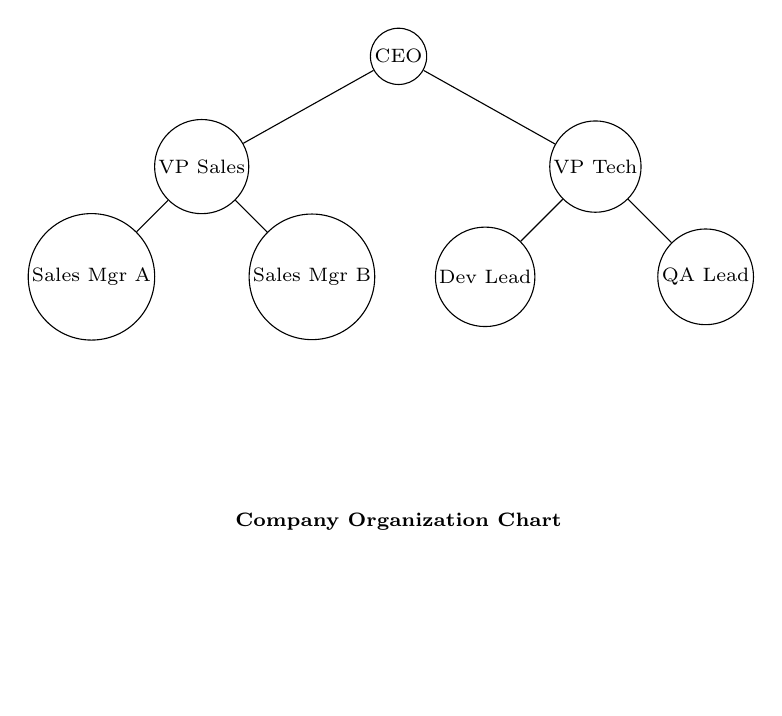
\begin{tikzpicture}[
    grow=down,
    level distance=1.4cm,
    level 1/.style={sibling distance=5cm},
    level 2/.style={sibling distance=2.8cm},
    every node/.style={
        draw,
        circle,
        minimum size=6mm,
        inner sep=1pt,
        font=\scriptsize
    },
    edge from parent/.style={draw,-}
]

\node {CEO}
    child { node {VP Sales}
        child { node {Sales Mgr A} }
        child { node {Sales Mgr B} }
    }
    child { node {VP Tech}
        child { node {Dev Lead} }
        child { node {QA Lead} }
    };

\node[below, draw=none] at (0,-3.8)
{\textbf{Company Organization Chart}};

\end{tikzpicture}
\end{center}

\textbf{Other examples:}
\begin{itemize}
    \item File systems (folders contain folders and files)
    \item Family trees (parents, children, descendants)
    \item HTML/DOM (tags contain other tags)
    \item Decision trees (if-then logic branches)
\end{itemize}

\begin{keyidea}
\textbf{Trees model relationships where:}
\begin{enumerate}
    \item One item is the "root" (starting point)
    \item Each item can have "children" (items below it)
    \item Each child has exactly one "parent" (item above it)
    \item No cycles (can't be your own ancestor!)
\end{enumerate}

Trees let us organize data in ways that linear structures can't!
\end{keyidea}

\section{First Principles: Tree Terminology}

\subsection{The Basic Structure}

\begin{center}
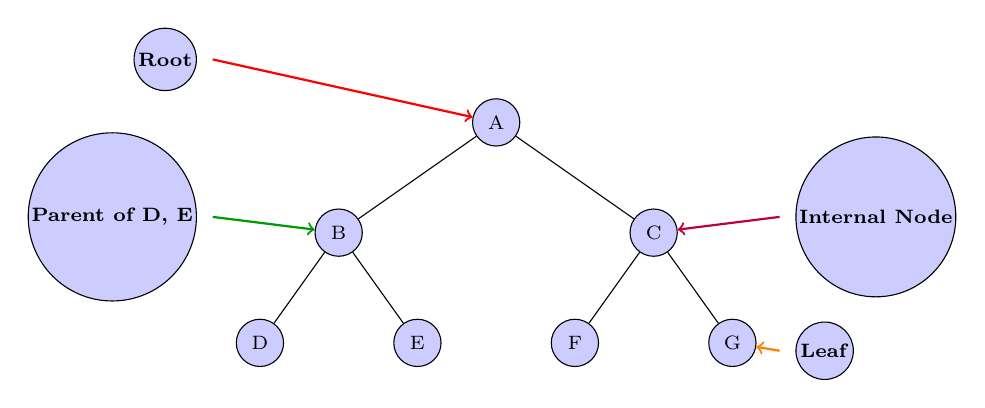
\begin{tikzpicture}[
    grow=down,
    level distance=1.4cm,
    level 1/.style={sibling distance=4cm},
    level 2/.style={sibling distance=2cm},
    every node/.style={
        circle,
        draw,
        minimum size=6mm,
        inner sep=1pt,
        fill=blue!20,
        font=\scriptsize
    },
    edge from parent/.style={draw,-}
]

% ---------------- Tree ----------------
\node (root) {A}
    child {node (b) {B}
        child {node (d) {D}}
        child {node (e) {E}}
    }
    child {node (c) {C}
        child {node (f) {F}}
        child {node (g) {G}}
    };

% ---------------- Left annotations ----------------
\node[anchor=east] at (-3.8,0.8) {\textbf{Root}};
\draw[->, red, thick] (-3.6,0.8) -- (root);

\node[anchor=east] at (-3.8,-1.2) {\textbf{Parent of D, E}};
\draw[->, green!60!black, thick] (-3.6,-1.2) -- (b);

% ---------------- Right annotations ----------------
\node[anchor=west] at (3.8,-1.2) {\textbf{Internal Node}};
\draw[->, purple, thick] (3.6,-1.2) -- (c);

\node[anchor=west] at (3.8,-2.9) {\textbf{Leaf}};
\draw[->, orange, thick] (3.6,-2.9) -- (g);

\end{tikzpicture}
\end{center}

\textbf{Vocabulary:}
\begin{itemize}
    \item \textbf{Root:} Top node (has no parent) — Node A
    \item \textbf{Parent:} Node directly above — B is parent of D and E
    \item \textbf{Child:} Node directly below — D and E are children of B
    \item \textbf{Siblings:} Nodes with same parent — D and E are siblings
    \item \textbf{Leaf:} Node with no children — D, E, F, G
    \item \textbf{Internal Node:} Node with at least one child — A, B, C
    \item \textbf{Subtree:} Tree formed by a node and its descendants
    \item \textbf{Edge:} Connection between parent and child
\end{itemize}

\subsection{Important Measurements}

\begin{center}
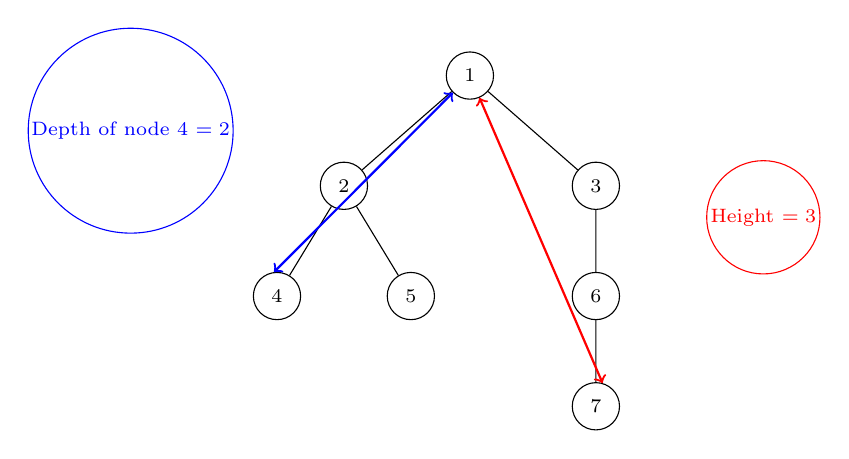
\begin{tikzpicture}[
    grow=down,
    level distance=1.4cm,
    level 1/.style={sibling distance=3.2cm},
    level 2/.style={sibling distance=1.7cm},
    every node/.style={
        circle,
        draw,
        minimum size=6mm,
        inner sep=1pt,
        font=\scriptsize
    },
    edge from parent/.style={draw,-}
]

% ---------------- Tree ----------------
\node (n1) {1}
    child { node (n2) {2}
        child { node (n4) {4} }
        child { node (n5) {5} }
    }
    child { node (n3) {3}
        child { node (n6) {6}
            child { node (n7) {7} }
        }
    };

% ---------------- Height annotation ----------------
\draw[<->, thick, red]
    ([xshift=2.8cm]n1) -- ([xshift=2.8cm]n7);
\node[red, anchor=west]
    at ([xshift=3.0cm,yshift=-1.8cm]n1) {Height $= 3$};

% ---------------- Depth annotation ----------------
\draw[<->, thick, blue]
    ([xshift=-2.8cm]n1) -- ([xshift=-2.8cm]n4);
\node[blue, anchor=east]
    at ([xshift=-3.0cm,yshift=-0.7cm]n1)
    {Depth of node 4 $= 2$};

\end{tikzpicture}
\end{center}

\begin{itemize}
    \item \textbf{Depth} of node: Distance from root (root has depth 0)
    \item \textbf{Height} of node: Distance to deepest leaf below it
    \item \textbf{Height} of tree: Height of root = max depth of any node
    \item \textbf{Level:} All nodes at same depth (level = depth)
\end{itemize}

\begin{keyidea}
\textbf{Depth:} How far DOWN from root? \\
\textbf{Height:} How far UP to reach it from deepest leaf?

Think of a building: depth is which floor you're on (from top), height is how many floors above you.
\end{keyidea}

\section{Binary Trees: At Most Two Children}

\subsection{Why Binary?}

A \textbf{binary tree} is a tree where each node has \textbf{at most 2 children}:
\begin{itemize}
    \item Left child
    \item Right child
\end{itemize}

\begin{center}
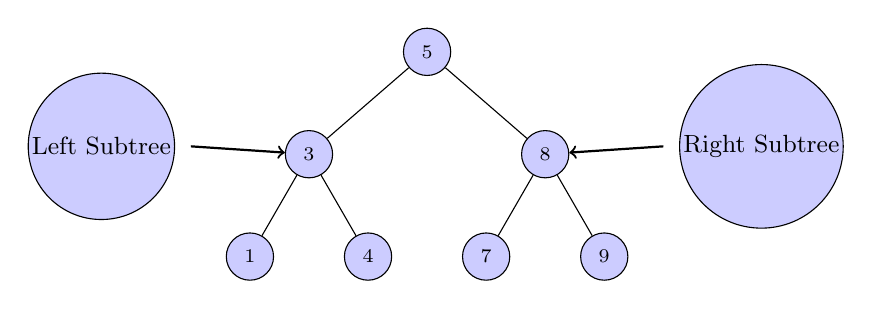
\begin{tikzpicture}[
    grow=down,
    level distance=1.3cm,
    level 1/.style={sibling distance=3cm},
    level 2/.style={sibling distance=1.5cm},
    every node/.style={
        circle,
        draw,
        minimum size=6mm,
        inner sep=1pt,
        fill=blue!20,
        font=\scriptsize
    },
    edge from parent/.style={draw,-}
]

% -------- Tree --------
\node (root) {5}
    child {node (L) {3}
        child {node {1}}
        child {node {4}}
    }
    child {node (R) {8}
        child {node {7}}
        child {node {9}}
    };

% -------- Left / Right labels --------
\node[anchor=east] at (-3.2,-1.2) {\small Left Subtree};
\draw[->, thick] (-3.0,-1.2) -- (L);

\node[anchor=west] at (3.2,-1.2) {\small Right Subtree};
\draw[->, thick] (3.0,-1.2) -- (R);

\end{tikzpicture}

\textbf{Binary Tree: Each node has $\le 2$ children}
\end{center}


\textbf{Why limit to 2?}
\begin{itemize}
    \item Simpler to implement and reason about
    \item Enables efficient search (Binary Search Trees!)
    \item Many algorithms naturally work with binary choices
\end{itemize}

\subsection{Binary Tree Node Implementation}

\begin{lstlisting}
class TreeNode:
    def __init__(self, data):
        self.data = data
        self.left = None   # Left child
        self.right = None  # Right child
    
    def __str__(self):
        return f"Node({self.data})"

# Build a simple tree
#       1
#      / \
#     2   3
#    / \
#   4   5

root = TreeNode(1)
root.left = TreeNode(2)
root.right = TreeNode(3)
root.left.left = TreeNode(4)
root.left.right = TreeNode(5)
\end{lstlisting}

\section{Tree Traversals: Visiting Every Node}

\textbf{Question:} How do we visit every node in a tree?

Unlike arrays (just loop), trees need special traversal strategies.

\subsection{The Three Main Traversals}

\begin{center}
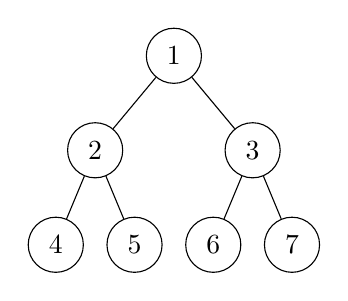
\begin{tikzpicture}[
    level distance=1.2cm,
    level 1/.style={sibling distance=2cm},
    level 2/.style={sibling distance=1cm},
    every node/.style={circle, draw, minimum size=0.7cm}
]
    \node {1}
        child {node {2}
            child {node {4}}
            child {node {5}}
        }
        child {node {3}
            child {node {6}}
            child {node {7}}
        };
\end{tikzpicture}

\vspace{0.5cm}

\textbf{Inorder (Left, Root, Right):} 4, 2, 5, 1, 6, 3, 7 \\
\textbf{Preorder (Root, Left, Right):} 1, 2, 4, 5, 3, 6, 7 \\
\textbf{Postorder (Left, Right, Root):} 4, 5, 2, 6, 7, 3, 1
\end{center}

\subsection{Inorder Traversal (Left → Root → Right)}

\begin{lstlisting}
def inorder(node):
    """
    Visit left subtree, then root, then right subtree.
    For BST: visits nodes in sorted order!
    """
    if node is None:
        return

    inorder(node.left)      # 1. Visit left
    print(node.data)        # 2. Process root
    inorder(node.right)     # 3. Visit right

# Trace for tree above:
# inorder(1) calls:
#   inorder(2) calls:
#     inorder(4) -> prints 4
#     prints 2
#     inorder(5) -> prints 5
#   prints 1
#   inorder(3) calls:
#     inorder(6) -> prints 6
#     prints 3
#     inorder(7) -> prints 7
\end{lstlisting}

\textbf{Time:} $O(n)$ — visit each node once \\
\textbf{Space:} $O(h)$ — recursion stack depth = height

\subsection{Preorder Traversal (Root → Left → Right)}

\begin{lstlisting}
def preorder(node):
    """
    Visit root first, then left, then right.
    Used to: copy tree, get prefix expression
    """
    if node is None:
        return
    
    print(node.data)        # 1. Process root
    preorder(node.left)     # 2. Visit left
    preorder(node.right)    # 3. Visit right

# Prints: 1, 2, 4, 5, 3, 6, 7
# (Root comes before its children)
\end{lstlisting}

\subsection{Postorder Traversal (Left → Right → Root)}

\begin{lstlisting}
def postorder(node):
    """
    Visit children first, then root.
    Used to: delete tree, get postfix expression
    """
    if node is None:
        return
    
    postorder(node.left)    # 1. Visit left
    postorder(node.right)   # 2. Visit right
    print(node.data)        # 3. Process root

# Prints: 4, 5, 2, 6, 7, 3, 1
# (Children come before parent)
\end{lstlisting}

\subsection{Level-Order Traversal (Breadth-First)}

Visit level by level, left to right — use a \textbf{queue}!

\begin{lstlisting}
from collections import deque

def level_order(root):
    """
    Visit tree level by level.
    Level 0: [1]
    Level 1: [2, 3]
    Level 2: [4, 5, 6, 7]
    """
    if root is None:
        return
    
    queue = deque([root])
    
    while queue:
        node = queue.popleft()
        print(node.data)
        
        if node.left:
            queue.append(node.left)
        if node.right:
            queue.append(node.right)

# Prints: 1, 2, 3, 4, 5, 6, 7
\end{lstlisting}

\begin{center}
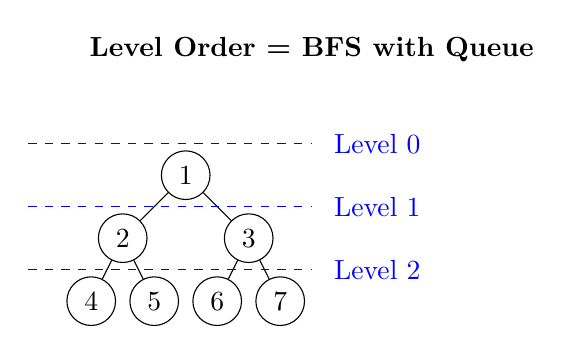
\begin{tikzpicture}[scale=0.8]
    \node at (4, 4) {\textbf{Level Order = BFS with Queue}};
    
    % Tree
    \node[circle, draw] (1) at (2, 2) {1};
    \node[circle, draw] (2) at (1, 1) {2};
    \node[circle, draw] (3) at (3, 1) {3};
    \node[circle, draw] (4) at (0.5, 0) {4};
    \node[circle, draw] (5) at (1.5, 0) {5};
    \node[circle, draw] (6) at (2.5, 0) {6};
    \node[circle, draw] (7) at (3.5, 0) {7};
    
    \draw (1) -- (2);
    \draw (1) -- (3);
    \draw (2) -- (4);
    \draw (2) -- (5);
    \draw (3) -- (6);
    \draw (3) -- (7);
    
    % Levels
    \draw[dashed, blue] (-0.5, 2.5) -- (4, 2.5);
    \node[blue, right] at (4.2, 2.5) {Level 0};
    \draw[dashed, blue] (-0.5, 1.5) -- (4, 1.5);
    \node[blue, right] at (4.2, 1.5) {Level 1};
    \draw[dashed, blue] (-0.5, 0.5) -- (4, 0.5);
    \node[blue, right] at (4.2, 0.5) {Level 2};
\end{tikzpicture}
\end{center}

\begin{keyidea}
\textbf{Traversal Choice Matters:}

\begin{itemize}
    \item \textbf{Inorder:} Get sorted values (in BST)
    \item \textbf{Preorder:} Copy tree structure
    \item \textbf{Postorder:} Delete tree (children before parent)
    \item \textbf{Level-order:} Process by levels, use queue
\end{itemize}

DFS (depth-first): inorder, preorder, postorder — use recursion/stack \\
BFS (breadth-first): level-order — use queue
\end{keyidea}

\section{Binary Search Trees (BST): The Ordered Tree}

\subsection{The BST Property}

A \textbf{Binary Search Tree} is a binary tree with a special ordering:

\begin{center}
\fbox{
\begin{minipage}{0.8\textwidth}
\textbf{BST Property:} For every node:
\begin{itemize}
    \item All values in \textbf{left} subtree $<$ node's value
    \item All values in \textbf{right} subtree $>$ node's value
\end{itemize}
\end{minipage}
}
\end{center}

\begin{center}
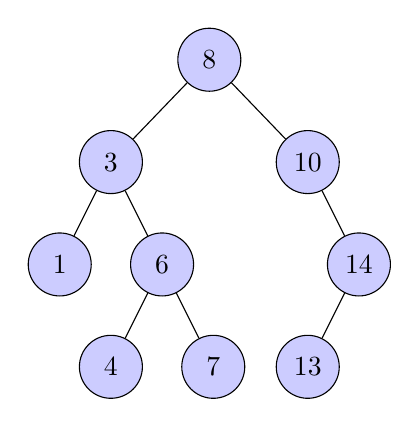
\begin{tikzpicture}[
    level distance=1.3cm,
    level 1/.style={sibling distance=2.5cm},
    level 2/.style={sibling distance=1.3cm},
    every node/.style={circle, draw, minimum size=0.8cm, fill=blue!20}
]
    \node {8}
        child {node {3}
            child {node {1}}
            child {node {6}
                child {node {4}}
                child {node {7}}
            }
        }
        child {node {10}
            child[missing]
            child {node {14}
                child {node {13}}
                child[missing]
            }
        };
\end{tikzpicture}

\vspace{0.3cm}
\textbf{Valid BST: Left < Parent < Right at every node}
\end{center}

\textbf{Why is this powerful?}

Like binary search on arrays, we can search in $O(\log n)$ time (in balanced trees)!

\subsection{BST Search: Like Binary Search}

\begin{lstlisting}
def search(node, target):
    """
    Search for target in BST.
    Time: O(h) where h = height
    In balanced tree: O(log n)
    In worst case (linear): O(n)
    """
    # Base case: not found
    if node is None:
        return False
    
    # Found it!
    if node.data == target:
        return True
    
    # Target is smaller, go left
    if target < node.data:
        return search(node.left, target)
    
    # Target is larger, go right
    else:
        return search(node.right, target)

# Iterative version (often preferred)
def search_iterative(node, target):
    """Same logic without recursion"""
    current = node
    
    while current is not None:
        if current.data == target:
            return True
        elif target < current.data:
            current = current.left
        else:
            current = current.right
    
    return False
\end{lstlisting}

\begin{center}
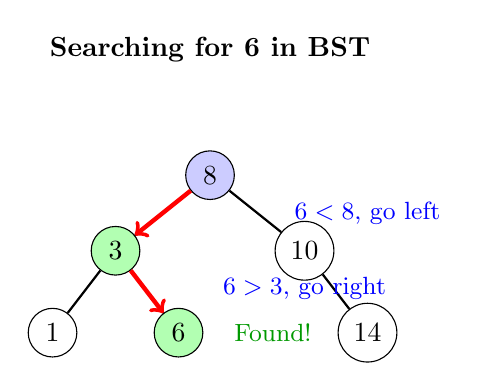
\begin{tikzpicture}[scale=0.8]
    \node at (3, 5) {\textbf{Searching for 6 in BST}};
    
    % Tree with search path highlighted
    \node[circle, draw, fill=blue!20] (8) at (3, 3) {8};
    \node[circle, draw, fill=green!30] (3) at (1.5, 1.8) {3};
    \node[circle, draw] (10) at (4.5, 1.8) {10};
    \node[circle, draw] (1) at (0.5, 0.5) {1};
    \node[circle, draw, fill=green!30] (6) at (2.5, 0.5) {6};
    \node[circle, draw] (14) at (5.5, 0.5) {14};
    
    \draw[thick] (8) -- (3);
    \draw[thick] (8) -- (10);
    \draw[thick] (3) -- (1);
    \draw[thick] (3) -- (6);
    \draw[thick] (10) -- (14);
    
    % Path arrows
    \draw[->, ultra thick, red] (8) -- (3);
    \draw[->, ultra thick, red] (3) -- (6);
    
    % Annotations - use $<$ and $>$ for proper symbols
    \node[font=\small, blue] at (5.5, 2.4) {$6 < 8$, go left};
    \node[font=\small, blue] at (4.5, 1.2) {$6 > 3$, go right};
    \node[font=\small, green!60!black] at (4, 0.5) {Found!};
\end{tikzpicture}

\vspace{0.3cm}
\small Only 3 comparisons instead of checking all 6 nodes!
\end{center}
\subsection{BST Insert: Maintain the Property}

\begin{lstlisting}
def insert(node, value):
    """
    Insert value into BST.
    Time: O(h) where h = height
    """
    # Base case: found insertion spot
    if node is None:
        return TreeNode(value)
    
    # Value already exists (no duplicates)
    if value == node.data:
        return node
    
    # Go left
    if value < node.data:
        node.left = insert(node.left, value)
    
    # Go right
    else:
        node.right = insert(node.right, value)
    
    return node

# Build BST by inserting: 8, 3, 10, 1, 6, 14
root = None
for value in [8, 3, 10, 1, 6, 14]:
    root = insert(root, value)
\end{lstlisting}

\begin{center}
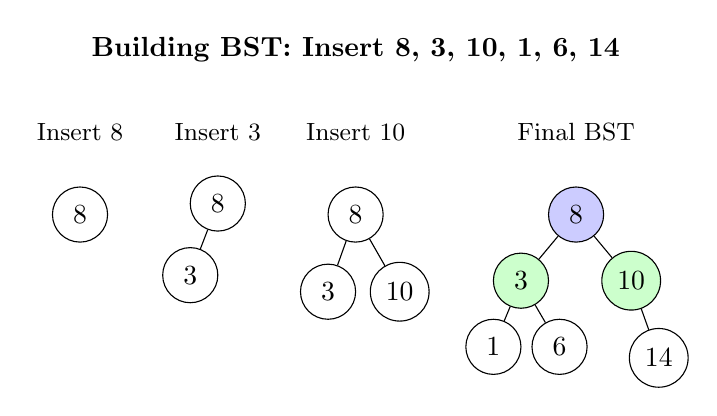
\begin{tikzpicture}[scale=0.7]
    \node at (5, 6.5) {\textbf{Building BST: Insert 8, 3, 10, 1, 6, 14}};
    
    % Step 1: Insert 8
    \node at (0, 5) {\small Insert 8};
    \node[circle, draw, minimum size=0.7cm] at (0, 3.5) {8};
    
    % Step 2: Insert 3
    \node at (2.5, 5) {\small Insert 3};
    \node[circle, draw, minimum size=0.7cm] (a) at (2.5, 3.7) {8};
    \node[circle, draw, minimum size=0.7cm] (a1) at (2, 2.4) {3};
    \draw (a) -- (a1);
    
    % Step 3: Insert 10
    \node at (5, 5) {\small Insert 10};
    \node[circle, draw, minimum size=0.7cm] (b) at (5, 3.5) {8};
    \node[circle, draw, minimum size=0.7cm] (b1) at (4.5, 2.1) {3};
    \node[circle, draw, minimum size=0.7cm] (b2) at (5.8, 2.1) {10};
    \draw (b) -- (b1);
    \draw (b) -- (b2);
    
    % Final tree
    \node at (9, 5) {\small Final BST};
    \node[circle, draw, fill=blue!20, minimum size=0.7cm] (c) at (9, 3.5) {8};
    \node[circle, draw, fill=green!20, minimum size=0.7cm] (d) at (8, 2.3) {3};
    \node[circle, draw, fill=green!20, minimum size=0.7cm] (e) at (10, 2.3) {10};
    \node[circle, draw, minimum size=0.7cm] (f) at (7.5, 1.1) {1};
    \node[circle, draw, minimum size=0.7cm] (g) at (8.7, 1.1) {6};
    \node[circle, draw, minimum size=0.7cm] (h) at (10.5, 0.9) {14};
    
    \draw (c) -- (d);
    \draw (c) -- (e);
    \draw (d) -- (f);
    \draw (d) -- (g);
    \draw (e) -- (h);
\end{tikzpicture}
\end{center}

\subsection{BST Delete: The Tricky Case}

Deleting has three cases:

\begin{enumerate}
    \item \textbf{Node is leaf:} Just remove it
    \item \textbf{Node has one child:} Replace node with its child
    \item \textbf{Node has two children:} Find successor, swap, delete successor
\end{enumerate}

\begin{lstlisting}
def find_min(node):
    """Find minimum value in tree (leftmost node)"""
    current = node
    while current.left:
        current = current.left
    return current

def delete(node, value):
    """
    Delete value from BST.
    Time: O(h)
    """
    if node is None:
        return None
    
    # Find the node to delete
    if value < node.data:
        node.left = delete(node.left, value)
    elif value > node.data:
        node.right = delete(node.right, value)
    else:
        # Found the node to delete!
        
        # Case 1: No children (leaf)
        if node.left is None and node.right is None:
            return None
        
        # Case 2: One child
        if node.left is None:
            return node.right
        if node.right is None:
            return node.left
        
        # Case 3: Two children
        # Find inorder successor (smallest in right subtree)
        successor = find_min(node.right)
        
        # Copy successor's value to this node
        node.data = successor.data
        
        # Delete the successor
        node.right = delete(node.right, successor.data)
    
    return node
\end{lstlisting}

\begin{center}
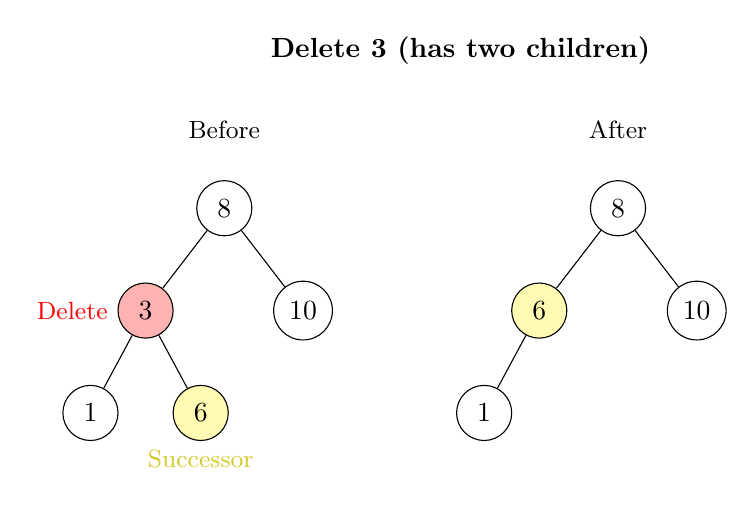
\begin{tikzpicture}[scale=1.0]
    \node at (5, 5.5) {\textbf{Delete 3 (has two children)}};
    
    % Before
    \node at (2, 4.5) {\small Before};
    \node[circle, draw, minimum size=0.7cm] (a) at (2, 3.5) {8};
    \node[circle, draw, fill=red!30, minimum size=0.7cm] (b) at (1, 2.2) {3};
    \node[circle, draw, minimum size=0.7cm] (c) at (3, 2.2) {10};
    \node[circle, draw, minimum size=0.7cm] (b1) at (0.3, 0.9) {1};
    \node[circle, draw, fill=yellow!30, minimum size=0.7cm] (b2) at (1.7, 0.9) {6};
    
    \draw (a) -- (b);
    \draw (a) -- (c);
    \draw (b) -- (b1);
    \draw (b) -- (b2);
    
    \node[red, left, font=\small] at (b.west) {Delete};
    \node[yellow!80!black, below, font=\small] at (b2.south) {Successor};
    
    % After
    \node at (7, 4.5) {\small After};
    \node[circle, draw, minimum size=0.7cm] (d) at (7, 3.5) {8};
    \node[circle, draw, fill=yellow!30, minimum size=0.7cm] (e) at (6, 2.2) {6};
    \node[circle, draw, minimum size=0.7cm] (f) at (8, 2.2) {10};
    \node[circle, draw, minimum size=0.7cm] (e1) at (5.3, 0.9) {1};
    
    \draw (d) -- (e);
    \draw (d) -- (f);
    \draw (e) -- (e1);
\end{tikzpicture}
\vspace{0.3cm}

\small Replace 3 with successor 6, delete original 6
\end{center}

\section{BST Operations Summary}

\begin{center}
\begin{tabular}{|l|c|c|}
\hline
\textbf{Operation} & \textbf{Average} & \textbf{Worst} \\
\hline
Search & $O(\log n)$ & $O(n)$ \\
Insert & $O(\log n)$ & $O(n)$ \\
Delete & $O(\log n)$ & $O(n)$ \\
Find Min/Max & $O(\log n)$ & $O(n)$ \\
Inorder Traversal & $O(n)$ & $O(n)$ \\
\hline
\end{tabular}
\end{center}

\textbf{Why worst case $O(n)$?}

If tree becomes unbalanced (skewed):
\begin{center}
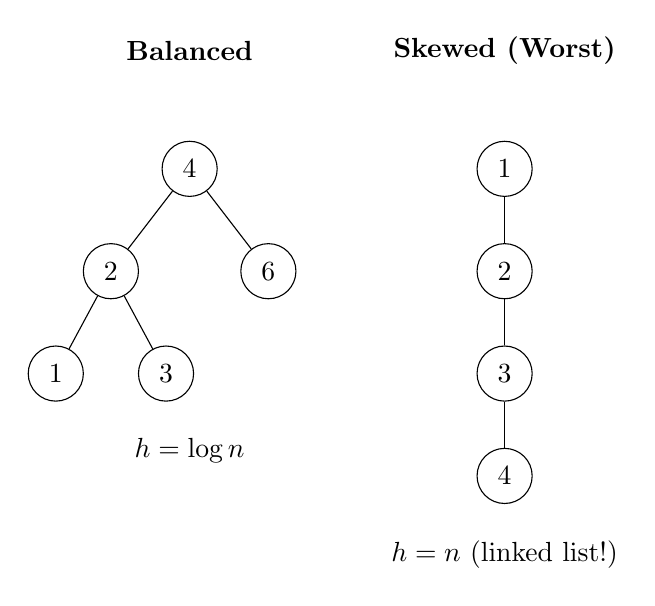
\begin{tikzpicture}[scale=1.0]
    % Balanced
    \node at (2, 5.5) {\textbf{Balanced}};
    \node[circle, draw, minimum size=0.7cm, fill=white] (a) at (2, 4) {4};
    \node[circle, draw, minimum size=0.7cm, fill=white] (b) at (1, 2.7) {2};
    \node[circle, draw, minimum size=0.7cm, fill=white] (c) at (3, 2.7) {6};
    \node[circle, draw, minimum size=0.7cm, fill=white] (d) at (0.3, 1.4) {1};
    \node[circle, draw, minimum size=0.7cm, fill=white] (e) at (1.7, 1.4) {3};
    
    \draw (a) -- (b);
    \draw (a) -- (c);
    \draw (b) -- (d);
    \draw (b) -- (e);
    
    \node[below] at (2, 0.7) {$h = \log n$};
    
    % Skewed
    \node at (6, 5.5) {\textbf{Skewed (Worst)}};
    \node[circle, draw, minimum size=0.7cm, fill=white] (f) at (6, 4) {1};
    \node[circle, draw, minimum size=0.7cm, fill=white] (g) at (6, 2.7) {2};
    \node[circle, draw, minimum size=0.7cm, fill=white] (h) at (6, 1.4) {3};
    \node[circle, draw, minimum size=0.7cm, fill=white] (i) at (6, 0.1) {4};
    
    \draw (f) -- (g);
    \draw (g) -- (h);
    \draw (h) -- (i);
    
    \node[below] at (6, -0.6) {$h = n$ (linked list!)};
\end{tikzpicture}
\end{center}

\begin{insight}
\textbf{The Balance Problem:}

BST performance depends on balance. Insert 1,2,3,4,5 in order → skewed tree!

\textbf{Solutions:}
\begin{itemize}
    \item AVL Trees (self-balancing, Chapter 18)
    \item Red-Black Trees (self-balancing, used in most libraries)
    \item Randomized insertion order
\end{itemize}

For now, understand: \textbf{balanced BST = $O(\log n)$, skewed BST = $O(n)$}
\end{insight}

\section{Common Tree Algorithms}

\subsection{Calculate Tree Height}

\begin{lstlisting}
def height(node):
    """
    Calculate height of tree.
    Height = longest path from node to leaf.
    """
    if node is None:
        return -1  # Or 0, depending on definition
    
    left_height = height(node.left)
    right_height = height(node.right)
    
    return 1 + max(left_height, right_height)

# For tree:     1
#              / \
#             2   3
# height = 1 + max(height(2), height(3))
#        = 1 + max(0, 0) = 1
\end{lstlisting}

\subsection{Count Nodes}

\begin{lstlisting}
def count_nodes(node):
    """Count total nodes in tree"""
    if node is None:
        return 0
    
    return 1 + count_nodes(node.left) + count_nodes(node.right)
\end{lstlisting}

\subsection{Check if Valid BST}

\begin{lstlisting}
def is_valid_bst(node, min_val=float('-inf'), max_val=float('inf')):
    """
    Check if tree is valid BST.
    Key insight: Each node must be within a valid range!
    """
    if node is None:
        return True
    
    # Check if current node violates BST property
    if node.data <= min_val or node.data >= max_val:
        return False
    
    # Check subtrees with updated ranges
    return (is_valid_bst(node.left, min_val, node.data) and
            is_valid_bst(node.right, node.data, max_val))

# Example: For node with value 5
#   Left subtree: all values must be in (-inf, 5)
#   Right subtree: all values must be in (5, inf)
\end{lstlisting}

\subsection{Lowest Common Ancestor (BST)}

\begin{lstlisting}
def lca_bst(root, p, q):
    """
    Find lowest common ancestor in BST.
    Beautiful use of BST property!
    """
    if root is None:
        return None
    
    # Both in left subtree
    if p < root.data and q < root.data:
        return lca_bst(root.left, p, q)
    
    # Both in right subtree
    if p > root.data and q > root.data:
        return lca_bst(root.right, p, q)
    
    # Split point: one left, one right (or one is root)
    return root

# In BST:    6
#           / \
#          2   8
#         / \ / \
#        0  4 7  9
#
# LCA(2, 8) = 6 (they split at 6)
# LCA(2, 4) = 2 (2 is ancestor of 4)
\end{lstlisting}

\section{Practice Problems}

\subsection{Problem 1: Maximum Depth}

\begin{lstlisting}
def max_depth(root):
    """
    Find maximum depth (height) of tree.
    Same as height function!
    """
    if root is None:
        return 0
    
    return 1 + max(max_depth(root.left), max_depth(root.right))
\end{lstlisting}

\subsection{Problem 2: Symmetric Tree}

\begin{lstlisting}
def is_symmetric(root):
    """
    Check if tree is mirror image of itself.
    Example:     1
                / \
               2   2
              / \ / \
             3  4 4  3  <- Symmetric
    """
    def is_mirror(left, right):
        # Both None
        if left is None and right is None:
            return True
        
        # One None, one not
        if left is None or right is None:
            return False
        
        # Values must match, and subtrees must mirror
        return (left.data == right.data and
                is_mirror(left.left, right.right) and
                is_mirror(left.right, right.left))
    
    if root is None:
        return True
    
    return is_mirror(root.left, root.right)
\end{lstlisting}

\subsection{Problem 3: Path Sum}

\begin{lstlisting}
def has_path_sum(root, target_sum):
    """
    Check if there's a root-to-leaf path that sums to target.
    Example:     5
                / \
               4   8
              /   / \
             11  13  4
            /  \      \
           7    2      1
    
    has_path_sum(22) = True (5->4->11->2)
    """
    if root is None:
        return False
    
    # Leaf node: check if it equals remaining sum
    if root.left is None and root.right is None:
        return root.data == target_sum
    
    # Check if either subtree has path
    remaining = target_sum - root.data
    return (has_path_sum(root.left, remaining) or
            has_path_sum(root.right, remaining))
\end{lstlisting}

\subsection{Problem 4: Kth Smallest in BST}

\begin{lstlisting}
def kth_smallest(root, k):
    """
    Find kth smallest element in BST.
    Key insight: Inorder traversal gives sorted order!
    """
    result = []
    
    def inorder(node):
        if node is None:
            return
        
        inorder(node.left)
        result.append(node.data)
        inorder(node.right)
    
    inorder(root)
    return result[k - 1]  # k is 1-indexed

# Better: stop early when we find kth element
def kth_smallest_optimized(root, k):
    stack = []
    current = root
    count = 0
    
    while stack or current:
        # Go left as far as possible
        while current:
            stack.append(current)
            current = current.left
        
        # Process node
        current = stack.pop()
        count += 1
        
        if count == k:
            return current.data
        
        # Go right
        current = current.right
    
    return None
\end{lstlisting}

\subsection{Problem 5: Serialize and Deserialize BST}

\begin{lstlisting}
def serialize(root):
    """
    Convert BST to string using preorder.
    Example: [2,1,3] -> "2,1,None,None,3,None,None"
    """
    if root is None:
        return "None"
    
    return f"{root.data},{serialize(root.left)},{serialize(root.right)}"

def deserialize(data):
    """Reconstruct BST from string"""
    def helper(values):
        val = next(values)
        
        if val == "None":
            return None
        
        node = TreeNode(int(val))
        node.left = helper(values)
        node.right = helper(values)
        
        return node
    
    values = iter(data.split(','))
    return helper(values)

# Test
root = TreeNode(2)
root.left = TreeNode(1)
root.right = TreeNode(3)

serialized = serialize(root)
print(serialized)  # "2,1,None,None,3,None,None"

new_root = deserialize(serialized)
print(new_root.data)  # 2
\end{lstlisting}

\section{Key Takeaways}

\begin{enumerate}
    \item \textbf{Trees model hierarchies}
    \begin{itemize}
        \item Root, parent, children, leaves
        \item Depth (from root), height (to deepest leaf)
    \end{itemize}
    
    \item \textbf{Binary trees: $\le 2$ children per node}
    \begin{itemize}
        \item Simpler structure, enables efficient algorithms
    \end{itemize}
    
    \item \textbf{Traversals visit all nodes}
    \begin{itemize}
        \item Inorder (Left-Root-Right): sorted for BST
        \item Preorder (Root-Left-Right): copy structure
        \item Postorder (Left-Right-Root): delete tree
        \item Level-order: BFS with queue
    \end{itemize}
    
    \item \textbf{BST property: Left $<$ Root $<$ Right}
    \begin{itemize}
        \item Enables $O(\log n)$ search/insert/delete
        \item Only if balanced! Skewed tree = $O(n)$
    \end{itemize}

    \item \textbf{Recursion is natural for trees}
    \begin{itemize}
        \item Each subtree is itself a tree
        \item Base case: empty tree (None)
        \item Recursive case: process root, recurse on children
    \end{itemize}
    
    \item \textbf{Balance matters}
    \begin{itemize}
        \item Balanced: $h = O(\log n)$ → fast operations
        \item Skewed: $h = O(n)$ → slow operations
        \item Self-balancing trees (AVL, Red-Black) maintain balance
    \end{itemize}
\end{enumerate}

\begin{insight}
Gilbert Strang's wisdom: "Trees are where recursion truly shines. Each tree is built from smaller trees — this self-similarity makes recursive solutions natural and elegant. When you see a tree problem, think: 'What do I do at this node? What do my left and right subtrees tell me?' Trust the recursion, and the solution unfolds beautifully."
\end{insight}

\section{Looking Ahead to Chapter 8}

Binary Search Trees give us $O(\log n)$ operations when balanced. But we can do even better for certain operations!

Next up: \textbf{Heaps and Priority Queues} — trees with a different property that gives us:
\begin{itemize}
    \item $O(1)$ access to minimum/maximum
    \item $O(\log n)$ insert and delete
    \item Perfect for: task scheduling, finding top K elements, sorting (heapsort)
\end{itemize}

Plus, heaps have a beautiful array representation — no pointers needed!

\vspace{1cm}

\begin{center}
\rule{0.5\textwidth}{0.4pt}

\textit{"A tree grows from its root, branches out, and reaches for the sky. So does understanding."}

\rule{0.5\textwidth}{0.4pt}
\end{center}
\pagebreak
\section{Chapter 8: Heaps and Priority Queues}
\subsection*{The Tree That Lives in an Array}

\begin{center}
\textit{"A heap is a tree with a promise: the parent is always greater (or smaller) than its children."}
\end{center}

\section{The Big Picture: What Problem Do Heaps Solve?}

Imagine you're managing a hospital emergency room. Patients arrive constantly, but you need to treat the \textbf{most urgent} patient next, not the one who arrived first.

\textbf{Options:}
\begin{itemize}
    \item \textbf{Unsorted array:} Find max = $O(n)$, insert = $O(1)$
    \item \textbf{Sorted array:} Find max = $O(1)$, insert = $O(n)$
    \item \textbf{BST:} Both = $O(\log n)$, but extra complexity
    \item \textbf{Heap:} Find max = $O(1)$, insert/delete = $O(\log n)$, simpler than BST!
\end{itemize}

\begin{keyidea}
\textbf{The Heap Promise:}

A heap gives us the \textbf{best of both worlds}:
\begin{enumerate}
    \item \textbf{Instant access} to max (or min) element: $O(1)$
    \item \textbf{Fast insert/delete:} $O(\log n)$
    \item \textbf{Simple structure:} Can store in array (no pointers!)
\end{enumerate}

Perfect for: Priority queues, top K elements, heap sort, scheduling
\end{keyidea}

\section{First Principles: The Heap Property}

\subsection{What IS a Heap?}

A \textbf{heap} is a \textbf{complete binary tree} with a special property:

\begin{center}
\fbox{
\begin{minipage}{0.85\textwidth}
\textbf{Max-Heap Property:} Every parent is $\geq$ its children \\
\textbf{Min-Heap Property:} Every parent is $\leq$ its children
\end{minipage}
}
\end{center}

\begin{center}
\begin{tikzpicture}[
    level distance=1.3cm,
    level 1/.style={sibling distance=2.5cm},
    level 2/.style={sibling distance=1.3cm},
    every node/.style={circle, draw, minimum size=0.8cm, fill=blue!20}
]
    % Max-Heap
    \node {50}
        child {node {30}
            child {node {10}}
            child {node {20}}
        }
        child {node {40}
            child {node {15}}
            child {node {25}}
        };
\end{tikzpicture}
\hspace{1cm}
\begin{tikzpicture}[
    level distance=1.3cm,
    level 1/.style={sibling distance=2.5cm},
    level 2/.style={sibling distance=1.3cm},
    every node/.style={circle, draw, minimum size=0.8cm, fill=green!20}
]
    % Min-Heap
    \node {5}
        child {node {10}
            child {node {30}}
            child {node {20}}
        }
        child {node {15}
            child {node {40}}
            child {node {25}}
        };
\end{tikzpicture}

\vspace{0.5cm}

\begin{minipage}{0.45\textwidth}
\centering
\textbf{Max-Heap: Parent $\geq$ Children}\\
{\color{red}\small Root = Maximum element!}
\end{minipage}
\hfill
\begin{minipage}{0.45\textwidth}
\centering
\textbf{Min-Heap: Parent $\leq$ Children}\\
{\color{red}\small Root = Minimum element!}
\end{minipage}
\end{center}

\textbf{Key differences from BST:}
\begin{itemize}
\item \textbf{BST:} Left $<$ Parent $<$ Right (ordered horizontally)
\item \textbf{Heap:} Parent vs Children only (ordered vertically)
\item \textbf{BST:} Can be any shape
\item \textbf{Heap:} Must be complete binary tree
\end{itemize}
\subsection{Complete Binary Tree: The Shape Rule}

A \textbf{complete binary tree} fills levels left to right, no gaps:

\begin{center}
\begin{tikzpicture}[scale=1.0]
    % -------- Complete tree --------
    \node at (2.5, 5.5) {\textbf{Complete $\checkmark$}};
    \node[circle, draw, fill=green!20, minimum size=0.7cm] (a1) at (2.5, 4) {1};
    \node[circle, draw, fill=green!20, minimum size=0.7cm] (a2) at (1.5, 2.7) {2};
    \node[circle, draw, fill=green!20, minimum size=0.7cm] (a3) at (3.5, 2.7) {3};
    \node[circle, draw, fill=green!20, minimum size=0.7cm] (a4) at (0.8, 1.4) {4};
    \node[circle, draw, fill=green!20, minimum size=0.7cm] (a5) at (2.2, 1.4) {5};
    
    \draw (a1) -- (a2);
    \draw (a1) -- (a3);
    \draw (a2) -- (a4);
    \draw (a2) -- (a5);
    
    \node[below, green!60!black, font=\small] at (2.5, 0.7) {Fills left to right};
    
    % -------- Not complete tree --------
    \node at (7, 5.5) {\textbf{Not Complete $\times$}};
    \node[circle, draw, fill=red!20, minimum size=0.7cm] (b1) at (7, 4) {1};
    \node[circle, draw, fill=red!20, minimum size=0.7cm] (b2) at (6, 2.7) {2};
    \node[circle, draw, fill=red!20, minimum size=0.7cm] (b3) at (8, 2.7) {3};
    \node[circle, draw, fill=red!20, minimum size=0.7cm] (b5) at (6.7, 1.4) {5};
    
    \draw (b1) -- (b2);
    \draw (b1) -- (b3);
    \draw (b2) -- (b5);
    
    \node[below, red, font=\small] at (7, 0.7) {Gap on left!};
\end{tikzpicture}
\end{center}

\textbf{Why complete?} Allows perfect array representation!

\section{The Magic: Heap in an Array}

\subsection{Array Representation}

Here's the beautiful part: we can store a complete binary tree in an array without pointers!

\begin{center}
\begin{tikzpicture}[scale=1.0]
    % Tree
    \node at (3.5, 6) {\textbf{Heap as Tree}};
    \node[circle, draw, fill=blue!20, minimum size=0.7cm] (0) at (3.5, 4.5) {50};
    \node[circle, draw, fill=blue!20, minimum size=0.7cm] (1) at (2, 3.2) {30};
    \node[circle, draw, fill=blue!20, minimum size=0.7cm] (2) at (5, 3.2) {40};
    \node[circle, draw, fill=blue!20, minimum size=0.7cm] (3) at (1, 1.9) {10};
    \node[circle, draw, fill=blue!20, minimum size=0.7cm] (4) at (3, 1.9) {20};
    \node[circle, draw, fill=blue!20, minimum size=0.7cm] (5) at (4, 1.9) {15};
    \node[circle, draw, fill=blue!20, minimum size=0.7cm] (6) at (6, 1.9) {25};
    
    \draw (0) -- (1);
    \draw (0) -- (2);
    \draw (1) -- (3);
    \draw (1) -- (4);
    \draw (2) -- (5);
    \draw (2) -- (6);
    
    % Array
    \node at (3.5, 0.8) {\textbf{Heap as Array}};
    \foreach \x/\val/\idx in {0/50/0, 1/30/1, 2/40/2, 3/10/3, 4/20/4, 5/15/5, 6/25/6} {
        \draw[thick] (\x*1, -0.3) rectangle (\x*1+1, 0.5);
        \node at (\x*1+0.5, 0.1) {\val};
        \node[below, font=\tiny] at (\x*1+0.5, -0.5) {\idx};
    }
    
    % Arrows showing mapping
    \draw[->, red, thick] (0) .. controls (2.5, 3) .. (0.5, 0.6);
    \draw[->, green!60!black, thick] (1) .. controls (1.5, 2) .. (1.5, 0.6);
    \draw[->, purple, thick] (2) .. controls (4.5, 2) .. (2.5, 0.6);
\end{tikzpicture}
\end{center}

\textbf{The Formula:} For node at index $i$:
\begin{itemize}
    \item \textbf{Left child:} $2i + 1$
    \item \textbf{Right child:} $2i + 2$
    \item \textbf{Parent:} $\lfloor (i-1)/2 \rfloor$
\end{itemize}

\begin{center}
\begin{tikzpicture}[scale=0.8]
    \node at (3.5, 4.5) {\textbf{Index Relationships}};
    
    % Array with relationships
    \foreach \x/\val/\idx in {0/50/0, 1/30/1, 2/40/2, 3/10/3, 4/20/4, 5/15/5, 6/25/6} {
        \draw[thick, fill=blue!20] (\x*1, 2) rectangle (\x*1+1, 3);
        \node at (\x*1+0.5, 2.5) {\val};
        \node[below, font=\small] at (\x*1+0.5, 1.8) {i=\idx};
    }
    
    % Show parent-child relationships
    \draw[->, thick, red] (0.5, 1.9) .. controls (0.5, 1.2) .. (1.5, 1.9);
    \node[red, font=\small] at (1, 0.8) {left child: $2i+1$};
    
    \draw[->, thick, red] (0.5, 1.9) .. controls (0.8, 0.8) .. (2.5, 1.9);
    \node[red, font=\small] at (2, 0.3) {right child: $2i+2$};
    
    \draw[<-, thick, green!60!black] (3.5, 3.1) .. controls (3.5, 3.6) .. (1.5, 3.1);
    \node[green!60!black, font=\small] at (2.5, 3.8) {parent: $(i-1)/2$};
\end{tikzpicture}
\end{center}

\begin{keyidea}
\textbf{Why This is Beautiful:}

No pointers needed! Just math to navigate:
\begin{itemize}
    \item Want left child of index 3? $2(3)+1 = 7$
    \item Want parent of index 5? $(5-1)/2 = 2$
    \item Cache-friendly: array access is fast
\end{itemize}

This is why heaps are so efficient!
\end{keyidea}

\section{Building a Max-Heap}

\subsection{Basic Heap Implementation}

\begin{lstlisting}
class MaxHeap:
    def __init__(self):
        self.heap = []
    
    def parent(self, i):
        """Get parent index"""
        return (i - 1) // 2
    
    def left_child(self, i):
        """Get left child index"""
        return 2 * i + 1
    
    def right_child(self, i):
        """Get right child index"""
        return 2 * i + 2
    
    def swap(self, i, j):
        """Swap two elements"""
        self.heap[i], self.heap[j] = self.heap[j], self.heap[i]
    
    def size(self):
        return len(self.heap)
    
    def is_empty(self):
        return len(self.heap) == 0
    
    def peek(self):
        """Get maximum element - O(1)"""
        if self.is_empty():
            raise IndexError("Heap is empty")
        return self.heap[0]
\end{lstlisting}

\subsection{Insert: Bubble Up}

When we insert a new element:
\begin{enumerate}
    \item Add it at the end (bottom-right of tree)
    \item \textbf{Bubble up:} Compare with parent, swap if larger
    \item Repeat until heap property restored
\end{enumerate}
\begin{center}
\begin{tikzpicture}[scale=1.0]
    \node at (4, 6) {\textbf{Insert 45 into Max-Heap}};
    
    % Step 1: Initial heap
    \node at (0, 5) {\small Step 1: Add};
    \node[circle, draw, minimum size=0.7cm] (a1) at (0, 3.8) {50};
    \node[circle, draw, minimum size=0.7cm] (a2) at (-0.8, 2.5) {30};
    \node[circle, draw, minimum size=0.7cm] (a3) at (0.8, 2.5) {40};
    \node[circle, draw, minimum size=0.7cm] (a4) at (-1.3, 1.2) {10};
    \node[circle, draw, minimum size=0.7cm] (a5) at (-0.3, 1.2) {20};
    \node[circle, draw, fill=yellow!40, minimum size=0.7cm] (a6) at (0.7, 1.2) {45};
    
    \draw (a1) -- (a2);
    \draw (a1) -- (a3);
    \draw (a2) -- (a4);
    \draw (a2) -- (a5);
    \draw (a3) -- (a6);
    
    \node[yellow!80!black, below, font=\small] at (a6.south) {New};
    
    % Step 2: Bubble up
    \node at (4, 5) {\small Step 2: Swap};
    \node[circle, draw, minimum size=0.7cm] (b1) at (4, 3.8) {50};
    \node[circle, draw, minimum size=0.7cm] (b2) at (3.2, 2.5) {30};
    \node[circle, draw, fill=yellow!40, minimum size=0.7cm] (b3) at (4.8, 2.5) {45};
    \node[circle, draw, minimum size=0.7cm] (b4) at (2.7, 1.2) {10};
    \node[circle, draw, minimum size=0.7cm] (b5) at (3.7, 1.2) {20};
    \node[circle, draw, minimum size=0.7cm] (b6) at (4.7, 1.2) {40};
    
    \draw (b1) -- (b2);
    \draw (b1) -- (b3);
    \draw (b2) -- (b4);
    \draw (b2) -- (b5);
    \draw (b3) -- (b6);
    
    \draw[->, red, ultra thick] (1.3, 2.5) -- (2.7, 2.5);
    \node[red, above, font=\small] at (2, 2.6) {$45 > 40$};
    
    % Step 3: Done
    \node at (8, 5) {\small Step 3: Done};
    \node[circle, draw, minimum size=0.7cm] (c1) at (8, 3.8) {50};
    \node[circle, draw, minimum size=0.7cm] (c2) at (7.2, 2.5) {30};
    \node[circle, draw, fill=green!30, minimum size=0.7cm] (c3) at (8.8, 2.5) {45};
    \node[circle, draw, minimum size=0.7cm] (c4) at (6.7, 1.2) {10};
    \node[circle, draw, minimum size=0.7cm] (c5) at (7.7, 1.2) {20};
    \node[circle, draw, minimum size=0.7cm] (c6) at (8.7, 1.2) {40};
    
    \draw (c1) -- (c2);
    \draw (c1) -- (c3);
    \draw (c2) -- (c4);
    \draw (c2) -- (c5);
    \draw (c3) -- (c6);
    
    \node[green!60!black, below, font=\small] at (c3.south) {$45 < 50$ \checkmark};
\end{tikzpicture}
\end{center}

\begin{lstlisting}
def insert(self, value):
    """
    Insert value into heap - O(log n)
    1. Add to end
    2. Bubble up until heap property satisfied
    """
    # Add to end
    self.heap.append(value)
    
    # Bubble up
    current = len(self.heap) - 1
    
    while current > 0:
        parent_idx = self.parent(current)
        
        # If current > parent, swap (max-heap)
        if self.heap[current] > self.heap[parent_idx]:
            self.swap(current, parent_idx)
            current = parent_idx
        else:
            break  # Heap property satisfied

# Usage
heap = MaxHeap()
for val in [50, 30, 40, 10, 20]:
    heap.insert(val)

heap.insert(45)  # Bubbles up from bottom
print(heap.heap)  # [50, 30, 45, 10, 20, 40]
\end{lstlisting}

\textbf{Time Complexity:} $O(\log n)$ — at most height swaps = $\log n$

\subsection{Extract Max: Bubble Down}

To remove the maximum (root):
\begin{enumerate}
    \item Replace root with last element
    \item \textbf{Bubble down:} Swap with larger child if needed
    \item Repeat until heap property restored
\end{enumerate}

\begin{center}
\begin{tikzpicture}[scale=0.9]
    \node at (5, 6.5) {\textbf{Extract Max from Heap}};
    
    % Step 1: Remove root
    \node at (0, 5.5) {\small Step 1};
    \node[circle, draw, fill=red!30, minimum size=0.7cm] (a1) at (0, 4.2) {50};
    \node[circle, draw, minimum size=0.7cm] (a2) at (-0.9, 3) {45};
    \node[circle, draw, minimum size=0.7cm] (a3) at (0.9, 3) {40};
    \node[circle, draw, minimum size=0.7cm] (a4) at (-1.4, 1.8) {30};
    \node[circle, draw, minimum size=0.7cm] (a5) at (-0.4, 1.8) {10};
    \node[circle, draw, fill=yellow!40, minimum size=0.7cm] (a6) at (0.7, 1.8) {20};
    
    \draw (a1) -- (a2);
    \draw (a1) -- (a3);
    \draw (a2) -- (a4);
    \draw (a2) -- (a5);
    \draw (a3) -- (a6);
    
    \node[red, above, font=\small] at (a1.north) {Remove};
    \node[yellow!80!black, below, font=\small] at (a6.south) {Move up};
    
    % Step 2: Replace with last
    \node at (3.8, 5.5) {\small Step 2};
    \node[circle, draw, fill=yellow!40, minimum size=0.7cm] (b1) at (3.8, 4.2) {20};
    \node[circle, draw, minimum size=0.7cm] (b2) at (2.9, 3) {45};
    \node[circle, draw, minimum size=0.7cm] (b3) at (4.7, 3) {40};
    \node[circle, draw, minimum size=0.7cm] (b4) at (2.4, 1.8) {30};
    \node[circle, draw, minimum size=0.7cm] (b5) at (3.4, 1.8) {10};
    
    \draw (b1) -- (b2);
    \draw (b1) -- (b3);
    \draw (b2) -- (b4);
    \draw (b2) -- (b5);
    
    \draw[->, red, ultra thick] (1.3, 4.2) -- (2.7, 4.2);
    
    % Step 3: Swap with larger child
    \node at (7.6, 5.5) {\small Step 3};
    \node[circle, draw, fill=green!30, minimum size=0.7cm] (c1) at (7.6, 4.2) {45};
    \node[circle, draw, fill=yellow!40, minimum size=0.7cm] (c2) at (6.7, 3) {20};
    \node[circle, draw, minimum size=0.7cm] (c3) at (8.5, 3) {40};
    \node[circle, draw, minimum size=0.7cm] (c4) at (6.2, 1.8) {30};
    \node[circle, draw, minimum size=0.7cm] (c5) at (7.2, 1.8) {10};
    
    \draw (c1) -- (c2);
    \draw (c1) -- (c3);
    \draw (c2) -- (c4);
    \draw (c2) -- (c5);
    
    \draw[->, red, ultra thick] (5.5, 4.2) -- (6.6, 4.2);
    \node[red, above, font=\small] at (6.05, 4.3) {$45 > 20$};
    
    % Step 4: Swap again
    \node at (11.4, 5.5) {\small Step 4: Done};
    \node[circle, draw, minimum size=0.7cm] (d1) at (11.4, 4.2) {45};
    \node[circle, draw, fill=green!30, minimum size=0.7cm] (d2) at (10.5, 3) {30};
    \node[circle, draw, minimum size=0.7cm] (d3) at (12.3, 3) {40};
    \node[circle, draw, fill=yellow!40, minimum size=0.7cm] (d4) at (10, 1.8) {20};
    \node[circle, draw, minimum size=0.7cm] (d5) at (11, 1.8) {10};
    
    \draw (d1) -- (d2);
    \draw (d1) -- (d3);
    \draw (d2) -- (d4);
    \draw (d2) -- (d5);
    
    \draw[->, red, ultra thick] (9.2, 3) -- (9.9, 3);
    \node[red, above, font=\small] at (9.55, 3.1) {$30 > 20$};
\end{tikzpicture}
\end{center}

\begin{lstlisting}
def extract_max(self):
    """
    Remove and return maximum element - O(log n)
    1. Save max (root)
    2. Replace root with last element
    3. Bubble down until heap property satisfied
    """
    if self.is_empty():
        raise IndexError("Heap is empty")
    
    # Save max
    max_val = self.heap[0]
    
    # Replace with last element
    self.heap[0] = self.heap[-1]
    self.heap.pop()
    
    # Bubble down
    if not self.is_empty():
        self._heapify_down(0)
    
    return max_val

def _heapify_down(self, i):
    """Bubble down from index i"""
    while True:
        largest = i
        left = self.left_child(i)
        right = self.right_child(i)
        
        # Check if left child is larger
        if left < len(self.heap) and self.heap[left] > self.heap[largest]:
            largest = left
        
        # Check if right child is larger
        if right < len(self.heap) and self.heap[right] > self.heap[largest]:
            largest = right
        
        # If largest is still i, we're done
        if largest == i:
            break
        
        # Swap and continue
        self.swap(i, largest)
        i = largest

# Usage
max_val = heap.extract_max()  # Returns 50
print(heap.heap)  # [45, 30, 40, 10, 20]
\end{lstlisting}

\textbf{Time Complexity:} $O(\log n)$ — at most height swaps

\section{Building a Heap from Array}

\subsection{Naive Approach: Insert One by One}

\begin{lstlisting}
def build_heap_naive(arr):
    """
    Build heap by inserting elements one by one.
    Time: O(n log n) - n inserts, each O(log n)
    """
    heap = MaxHeap()
    for val in arr:
        heap.insert(val)  # O(log n) each
    return heap
\end{lstlisting}

\subsection{Smart Approach: Heapify Bottom-Up}

Better algorithm: Start from bottom, heapify up:

\begin{lstlisting}
def build_heap_optimal(arr):
    """
    Build heap using heapify from bottom up.
    Time: O(n) - faster than O(n log n)!
    
    Key insight: Start from last non-leaf node,
    work backwards, heapify each.
    """
    heap = MaxHeap()
    heap.heap = arr.copy()
    
    # Last non-leaf node is at index (n//2 - 1)
    start = len(arr) // 2 - 1
    
    # Heapify from bottom to top
    for i in range(start, -1, -1):
        heap._heapify_down(i)
    
    return heap

# Example
arr = [3, 9, 2, 1, 4, 5]
heap = build_heap_optimal(arr)
print(heap.heap)  # [9, 4, 5, 1, 3, 2] - valid max-heap!
\end{lstlisting}

\begin{keyidea}
\textbf{Why is heapify $O(n)$?}

Mathematical proof (beautiful!):
\begin{itemize}
    \item Leaves (half the nodes): 0 work
    \item Level above: at most 1 swap per node
    \item Level above that: at most 2 swaps per node
    \item Root: at most $\log n$ swaps (but only 1 node!)
\end{itemize}

Sum: $\sum_{h=0}^{\log n} \frac{n}{2^{h+1}} \cdot h = O(n)$

Bottom-up heapify is LINEAR time — amazing!
\end{keyidea}

\section{Priority Queue: The Abstract Interface}

A \textbf{priority queue} is an abstract data type (like stack/queue) where each element has a priority:

\begin{center}
\begin{tabular}{|l|c|}
\hline
\textbf{Operation} & \textbf{Time (Heap)} \\
\hline
Insert & $O(\log n)$ \\
Get Max/Min & $O(1)$ \\
Extract Max/Min & $O(\log n)$ \\
Peek & $O(1)$ \\
\hline
\end{tabular}
\end{center}

\begin{lstlisting}
# Python's heapq module implements min-heap
import heapq

# Create empty heap
heap = []

# Insert elements - O(log n) each
heapq.heappush(heap, 5)
heapq.heappush(heap, 3)
heapq.heappush(heap, 7)
heapq.heappush(heap, 1)

print(heap)  # [1, 3, 7, 5] - min-heap array representation

# Peek at minimum - O(1)
print(heap[0])  # 1

# Extract minimum - O(log n)
min_val = heapq.heappop(heap)
print(min_val)  # 1
print(heap)     # [3, 5, 7]

# Build heap from list - O(n)
data = [9, 5, 6, 2, 3]
heapq.heapify(data)  # In-place!
print(data)  # [2, 3, 6, 9, 5] - valid min-heap

# For max-heap, use negative values
max_heap = []
for val in [3, 7, 1, 9]:
    heapq.heappush(max_heap, -val)

max_val = -heapq.heappop(max_heap)  # 9
\end{lstlisting}

\section{Heap Sort: Sorting with Heaps}

\subsection{The Algorithm}

\begin{enumerate}
    \item Build max-heap from array: $O(n)$
    \item Repeatedly extract max: $n \times O(\log n)$
    \item Total: $O(n \log n)$ — guaranteed!
\end{enumerate}

\begin{lstlisting}
def heap_sort(arr):
    """
    Sort array using heap.
    Time: O(n log n) - guaranteed (unlike quicksort)
    Space: O(1) - in-place (unlike mergesort)
    """
    n = len(arr)
    
    # Build max-heap - O(n)
    for i in range(n // 2 - 1, -1, -1):
        heapify_down(arr, n, i)
    
    # Extract elements one by one - O(n log n)
    for i in range(n - 1, 0, -1):
        # Swap max (root) with last element
        arr[0], arr[i] = arr[i], arr[0]
        
        # Heapify reduced heap
        heapify_down(arr, i, 0)

def heapify_down(arr, n, i):
    """Heapify subtree rooted at i with size n"""
    largest = i
    left = 2 * i + 1
    right = 2 * i + 2
    
    if left < n and arr[left] > arr[largest]:
        largest = left
    
    if right < n and arr[right] > arr[largest]:
        largest = right
    
    if largest != i:
        arr[i], arr[largest] = arr[largest], arr[i]
        heapify_down(arr, n, largest)

# Test
arr = [12, 11, 13, 5, 6, 7]
heap_sort(arr)
print(arr)  # [5, 6, 7, 11, 12, 13]
\end{lstlisting}
\pagebreak
\textbf{Heap Sort Advantages:}
\begin{itemize}
    \item $O(n \log n)$ worst case (unlike quicksort's $O(n^2)$)
    \item $O(1)$ space (unlike mergesort's $O(n)$)
    \item No recursion stack
\end{itemize}

\textbf{Disadvantages:}
\begin{itemize}
    \item Not stable (equal elements may swap order)
    \item Poor cache locality (random memory access)
    \item Slower than quicksort in practice
\end{itemize}

\section{Common Heap Applications}

\subsection{Application 1: Top K Elements}

Find K largest elements in stream:

\begin{lstlisting}
import heapq

def find_k_largest(stream, k):
    """
    Find k largest elements efficiently.
    
    Key insight: Use min-heap of size k!
    - If new element > min of heap, replace min
    - Heap always contains k largest seen so far
    
    Time: O(n log k) - much better than O(n log n) sorting!
    Space: O(k)
    """
    min_heap = []
    
    for num in stream:
        if len(min_heap) < k:
            heapq.heappush(min_heap, num)
        elif num > min_heap[0]:
            heapq.heapreplace(min_heap, num)  # Pop and push in one
    
    return sorted(min_heap, reverse=True)

# Example
stream = [3, 1, 5, 12, 2, 11, 8, 7]
print(find_k_largest(stream, 3))  # [12, 11, 8]
\end{lstlisting}
\begin{center}
\begin{tikzpicture}[scale=0.9]

    % Title (fixed at top)
    \node[font=\bfseries] (title) at (0, 4.8) {Finding Top 3 with Min-Heap};

    % Main content block
    \node[align=left, font=\small, anchor=north west] (content) at (-1.5, 4) {
        Stream: 3, 1, 5, 12, 2, 11 \\[0.35cm]
        After 3: \quad heap = [3] \\[0.25cm]
        After 1: \quad heap = [1, 3] \\[0.25cm]
        After 5: \quad heap = [1, 3, 5] \\[0.25cm]
        After 12: \quad heap = [3, 5, 12] \quad {\color{red}(replaced 1)} \\[0.25cm]
        After 2: \quad heap = [3, 5, 12] \quad {\color{blue}(2 $<$ 3, skip)} \\[0.25cm]
        After 11: \quad heap = [5, 11, 12] \quad {\color{red}(replaced 3)}
    };

    % Bottom note (properly spaced, no overlap)
    \node[font=\small, below=0.6cm of content.south west, anchor=west]
    {Heap always has $k=3$ largest elements};

\end{tikzpicture}
\end{center}

\subsection{Application 2: Merge K Sorted Lists}

\begin{lstlisting}
import heapq

def merge_k_sorted_lists(lists):
    """
    Merge k sorted lists efficiently.
    
    Naive: Compare all heads repeatedly - O(nk)
    Smart: Use min-heap - O(n log k)
    
    where n = total elements, k = number of lists
    """
    min_heap = []
    result = []
    
    # Initialize heap with first element from each list
    # Store (value, list_index, element_index)
    for i, lst in enumerate(lists):
        if lst:
            heapq.heappush(min_heap, (lst[0], i, 0))
    
    # Extract min and add next from same list
    while min_heap:
        val, list_idx, elem_idx = heapq.heappop(min_heap)
        result.append(val)
        
        # Add next element from same list
        if elem_idx + 1 < len(lists[list_idx]):
            next_val = lists[list_idx][elem_idx + 1]
            heapq.heappush(min_heap, (next_val, list_idx, elem_idx + 1))
    
    return result

# Test
lists = [
    [1, 4, 7],
    [2, 5, 8],
    [3, 6, 9]
]
print(merge_k_sorted_lists(lists))
# [1, 2, 3, 4, 5, 6, 7, 8, 9]
\end{lstlisting}

\subsection{Application 3: Median from Data Stream}

\begin{lstlisting}
import heapq

class MedianFinder:
    """
    Find median efficiently from data stream.
    
    Brilliant idea: Use TWO heaps!
    - Max-heap for smaller half
    - Min-heap for larger half
    - Keep sizes balanced
    
    Median is either:
    - Top of max-heap (if odd total)
    - Average of tops (if even total)
    """
    def __init__(self):
        self.small = []  # Max-heap (use negative values)
        self.large = []  # Min-heap
    
    def add_num(self, num):
        """Add number - O(log n)"""
        # Add to max-heap (small half)
        heapq.heappush(self.small, -num)
        
        # Balance: largest of small must be <= smallest of large
        if self.small and self.large and (-self.small[0] > self.large[0]):
            val = -heapq.heappop(self.small)
            heapq.heappush(self.large, val)
        
        # Balance sizes: differ by at most 1
        if len(self.small) > len(self.large) + 1:
            val = -heapq.heappop(self.small)
            heapq.heappush(self.large, val)
        
        if len(self.large) > len(self.small):
            val = heapq.heappop(self.large)
            heapq.heappush(self.small, -val)
    
    def find_median(self):
        """Get median - O(1)"""
        if len(self.small) > len(self.large):
            return -self.small[0]
        return (-self.small[0] + self.large[0]) / 2.0

# Test
mf = MedianFinder()
mf.add_num(1)
mf.add_num(2)
print(mf.find_median())  # 1.5
mf.add_num(3)
print(mf.find_median())  # 2.0
\end{lstlisting}

\begin{center}
\begin{tikzpicture}[scale=0.85]

    % Title
    \node[font=\bfseries] at (4, 5.2) {Two Heaps for Median};

    % Max-heap (small)
    \node[font=\small] at (1.5, 3.6) {Max-Heap (small)};
    \draw[thick, fill=blue!20] (0.5, 2) rectangle (2.5, 3);
    \node at (1.5, 2.5) {[1, 2, 3]};
    \node[font=\small] at (1.5, 1.7) {Top = 3};

    % Min-heap (large)
    \node[font=\small] at (6.5, 3.6) {Min-Heap (large)};
    \draw[thick, fill=green!20] (5.5, 2) rectangle (7.5, 3);
    \node at (6.5, 2.5) {[5, 6, 7]};
    \node[font=\small] at (6.5, 1.7) {Top = 5};

    % Arrow (slightly lower)
    \draw[->, ultra thick, red] (2.6, 2.35) -- (5.4, 2.35)
        node[midway, above=10pt, font=\small, red]
        {\textbf{Median = $(3+5)/2 = 4$}};

    % Bottom note
    \node[font=\small] at (4, 0.7)
    {Small half $\le$ Median $\le$ Large half};

\end{tikzpicture}
\end{center}

\section{Practice Problems}

\subsection{Problem 1: Kth Largest Element}

\begin{lstlisting}
def find_kth_largest(nums, k):
    """
    Find kth largest element.
    Multiple approaches:
    
    1. Sort: O(n log n)
    2. Min-heap of size k: O(n log k)
    3. Quickselect: O(n) average
    """
    # Approach 2: Min-heap
    import heapq
    
    heap = nums[:k]
    heapq.heapify(heap)  # O(k)
    
    for num in nums[k:]:  # O((n-k) log k)
        if num > heap[0]:
            heapq.heapreplace(heap, num)
    
    return heap[0]

# Test
nums = [3, 2, 1, 5, 6, 4]
print(find_kth_largest(nums, 2))  # 5
\end{lstlisting}

\subsection{Problem 2: Task Scheduler}

\begin{lstlisting}
import heapq
from collections import Counter

def least_interval(tasks, n):
    """
    Schedule tasks with cooldown n.
    Same task must wait n intervals.
    
    Example: tasks = ["A","A","A","B","B","B"], n = 2
    Output: 8  (A -> B -> idle -> A -> B -> idle -> A -> B)
    
    Use max-heap to always schedule most frequent task!
    """
    # Count frequencies
    freq = Counter(tasks)
    
    # Max-heap (use negative frequencies)
    heap = [-count for count in freq.values()]
    heapq.heapify(heap)
    
    time = 0
    
    while heap:
        temp = []
        
        # Process n+1 tasks (or fewer if heap small)
        for _ in range(n + 1):
            if heap:
                count = heapq.heappop(heap)
                if count < -1:
                    temp.append(count + 1)
            time += 1
            
            if not heap and not temp:
                break
        
        # Put back remaining tasks
        for count in temp:
            heapq.heappush(heap, count)
    
    return time

# Test
tasks = ["A","A","A","B","B","B"]
print(least_interval(tasks, 2))  # 8
\end{lstlisting}

\subsection{Problem 3: Ugly Number II}

\begin{lstlisting}
import heapq

def nth_ugly_number(n):
    """
    Find nth ugly number (only factors 2, 3, 5).
    Sequence: 1, 2, 3, 4, 5, 6, 8, 9, 10, 12...
    
    Use min-heap to generate in order!
    """
    heap = [1]
    seen = {1}
    ugly = 1
    
    for _ in range(n):
        ugly = heapq.heappop(heap)
        
        # Generate next candidates
        for factor in [2, 3, 5]:
            new_ugly = ugly * factor
            if new_ugly not in seen:
                seen.add(new_ugly)
                heapq.heappush(heap, new_ugly)
    
    return ugly

# Test
print(nth_ugly_number(10))  # 12
print(nth_ugly_number(15))  # 24
\end{lstlisting}

\section{Min-Heap vs Max-Heap: When to Use Which?}

\begin{center}
\begin{tabular}{|l|c|c|}
\hline
\textbf{Use Case} & \textbf{Min-Heap} & \textbf{Max-Heap} \\
\hline
Find minimum & $\checkmark$ &  \\
Find maximum &  & $\checkmark$ \\
Find k largest & $\checkmark$ &  \\
Find k smallest &  & $\checkmark$ \\
Dijkstra's algorithm & $\checkmark$ &  \\
Heap sort (ascending) &  & $\checkmark$ \\
Priority queue (high first) &  & $\checkmark$ \\
Priority queue (low first) & $\checkmark$ &  \\
\hline
\end{tabular}
\end{center}

\begin{keyidea}
\textbf{Counterintuitive Trick:}

To find k \textbf{largest}, use \textbf{min-heap} of size k! \\
To find k \textbf{smallest}, use \textbf{max-heap} of size k!

Why? Keep the "boundary" element at top for easy comparison.
\end{keyidea}

\section{Heap Operations Summary}

\begin{center}
\begin{tabular}{|l|c|c|}
\hline
\textbf{Operation} & \textbf{Time} & \textbf{Space} \\
\hline
Get min/max & $O(1)$ & $O(1)$ \\
Insert & $O(\log n)$ & $O(1)$ \\
Extract min/max & $O(\log n)$ & $O(1)$ \\
Build heap (heapify) & $O(n)$ & $O(1)$ \\
Heap sort & $O(n \log n)$ & $O(1)$ \\
\hline
\end{tabular}
\end{center}

\section{Key Takeaways}

\begin{enumerate}
    \item \textbf{Heap = Complete binary tree + heap property}
    \begin{itemize}
        \item Max-heap: Parent $\geq$ children
        \item Min-heap: Parent $\leq$ children
    \end{itemize}
    
    \item \textbf{Array representation is beautiful}
    \begin{itemize}
        \item Left child: $2i + 1$
        \item Right child: $2i + 2$
        \item Parent: $(i-1)/2$
        \item No pointers needed!
    \end{itemize}
    
    \item \textbf{Two key operations}
    \begin{itemize}
        \item Insert: Add to end, bubble up
        \item Extract: Replace root with last, bubble down
        \item Both $O(\log n)$
    \end{itemize}
    
    \item \textbf{Building heap is $O(n)$}
    \begin{itemize}
        \item Heapify bottom-up
        \item NOT $O(n \log n)$ — linear!
    \end{itemize}
    
    \item \textbf{Perfect for priority queues}
    \begin{itemize}
        \item Always access highest/lowest priority in $O(1)$
        \item Insert/delete in $O(\log n)$
    \end{itemize}
    
    \item \textbf{Heap sort: $O(n \log n)$ guaranteed}
    \begin{itemize}
        \item In-place: $O(1)$ space
        \item Not stable
        \item Slower than quicksort in practice
    \end{itemize}
    
    \item \textbf{Common patterns}
    \begin{itemize}
        \item Top K elements: min-heap of size k
        \item Merge k sorted: min-heap
        \item Running median: two heaps
    \end{itemize}
\end{enumerate}

\begin{insight}
Gilbert Strang's wisdom: "The heap is elegant in its simplicity. A tree that lives in an array. A guarantee that the best is always on top. And operations that dance up and down in logarithmic time. When you need the best element repeatedly, think heap. When you need to sort in-place with guaranteed performance, think heap sort. The heap is the unsung hero of efficient algorithms."
\end{insight}

\section{Looking Ahead to Chapter 9}

We've now mastered fundamental data structures:
\begin{itemize}
    \item Linear: Arrays, lists, stacks, queues
    \item Associative: Hash tables
    \item Hierarchical: Trees, BSTs, heaps
\end{itemize}

Next up: \textbf{Graphs} — the most general structure of all!

Graphs model:
\begin{itemize}
    \item Social networks (friends, followers)
    \item Maps and navigation (cities, roads)
    \item Dependencies (tasks, prerequisites)
    \item The internet itself!
\end{itemize}

Get ready for BFS, DFS, shortest paths, and the beautiful algorithms that work on graphs!

\vspace{1cm}

\begin{center}
\rule{0.5\textwidth}{0.4pt}

\textit{"In a heap, the best always rises to the top. Mathematics guarantees it."}

\rule{0.5\textwidth}{0.4pt}
\end{center}
\pagebreak
\section{Chapter 9: Graphs - Representation and Basics}
\subsection*{The Most General Data Structure}

\begin{center}
\textit{"A graph is everything connected to everything else, in whatever way you want."}
\end{center}

\section{The Big Picture: What ARE Graphs?}

Every data structure we've studied is actually a special case of a graph:
\begin{center}
\begin{tikzpicture}[scale=0.9]
    % Array/List
    \node at (0, 3.5) {\textbf{Array/List}};
    \foreach \x in {0,1,2,3} {
        \node[circle, draw, fill=blue!20, minimum size=0.6cm] (n\x) at (\x*1, 2) {};
    }
    \draw[->, thick] (n0) -- (n1);
    \draw[->, thick] (n1) -- (n2);
    \draw[->, thick] (n2) -- (n3);
    \node[below] at (1.5, 1.3) {\small Linear chain};
    
    % Tree
    \node at (6, 3.5) {\textbf{Tree}};
    \node[circle, draw, fill=green!20, minimum size=0.5cm] (t1) at (6, 2) {};
    \node[circle, draw, fill=green!20, minimum size=0.5cm] (t2) at (5.3, 1.2) {};
    \node[circle, draw, fill=green!20, minimum size=0.5cm] (t3) at (6.7, 1.2) {};
    \node[circle, draw, fill=green!20, minimum size=0.5cm] (t4) at (5, 0.4) {};
    \node[circle, draw, fill=green!20, minimum size=0.5cm] (t5) at (5.6, 0.4) {};
    
    \draw (t1) -- (t2);
    \draw (t1) -- (t3);
    \draw (t2) -- (t4);
    \draw (t2) -- (t5);
    \node[below] at (6, -0.2) {\small Hierarchy, no cycles};
    
    % General Graph
    \node at (10.5, 3.5) {\textbf{Graph}};
    \node[circle, draw, fill=yellow!30, minimum size=0.5cm] (g1) at (10, 2) {};
    \node[circle, draw, fill=yellow!30, minimum size=0.5cm] (g2) at (11, 2) {};
    \node[circle, draw, fill=yellow!30, minimum size=0.5cm] (g3) at (10, 0.8) {};
    \node[circle, draw, fill=yellow!30, minimum size=0.5cm] (g4) at (11, 0.8) {};
    
    \draw (g1) -- (g2);
    \draw (g1) -- (g3);
    \draw (g2) -- (g4);
    \draw (g3) -- (g4);
    \draw (g1) -- (g4);
    \node[below] at (10.5, -0.2) {\small Any connections!};
\end{tikzpicture}
\end{center}

\begin{keyidea}
A \textbf{graph} $G = (V, E)$ consists of:
\begin{itemize}
    \item \textbf{Vertices (V):} Nodes/points (like cities, people, web pages)
    \item \textbf{Edges (E):} Connections between vertices (like roads, friendships, links)
\end{itemize}

\textbf{No restrictions!} Any vertex can connect to any other vertex (or even itself).

This makes graphs the most \textbf{general} and \textbf{powerful} data structure.
\end{keyidea}

\section{First Principles: Types of Graphs}

\subsection{Undirected vs Directed Graphs}

\begin{center}
\begin{tikzpicture}[scale=0.8]
    % Undirected
    \node at (2, 4) {\textbf{Undirected Graph}};
    \node[circle, draw, fill=blue!20] (A) at (1, 2.5) {A};
    \node[circle, draw, fill=blue!20] (B) at (3, 2.5) {B};
    \node[circle, draw, fill=blue!20] (C) at (2, 1) {C};
    
    \draw[thick] (A) -- (B);
    \draw[thick] (B) -- (C);
    \draw[thick] (C) -- (A);
    
    \node[below] at (1, 0.3) {Two-way streets};
    \node[below, font=\small] at (1, -0.2) {Facebook friends};
    
    % Directed
    \node at (7, 4) {\textbf{Directed Graph (Digraph)}};
    \node[circle, draw, fill=green!20] (D) at (6, 2.5) {A};
    \node[circle, draw, fill=green!20] (E) at (8, 2.5) {B};
    \node[circle, draw, fill=green!20] (F) at (7, 1) {C};
    
    \draw[->, thick] (D) -- (E);
    \draw[->, thick] (E) -- (F);
    \draw[->, thick] (F) -- (D);
    \draw[->, thick] (E) to[bend left] (D);
    
    \node[below] at (7, 0.3) {One-way streets};
    \node[below, font=\small] at (7, -0.2) {Twitter followers};
\end{tikzpicture}
\end{center}

\textbf{Undirected:} Edge $(u,v)$ means $u \leftrightarrow v$ (bidirectional) \\
\textbf{Directed:} Edge $(u,v)$ means $u \to v$ (one-way)

\subsection{Weighted vs Unweighted Graphs}

\begin{center}
\begin{tikzpicture}[scale=0.8]
    % Unweighted
    \node at (2, 4) {\textbf{Unweighted}};
    \node[circle, draw, fill=blue!20] (A) at (1, 2.5) {A};
    \node[circle, draw, fill=blue!20] (B) at (3, 2.5) {B};
    \node[circle, draw, fill=blue!20] (C) at (2, 1) {C};
    
    \draw[thick] (A) -- (B);
    \draw[thick] (B) -- (C);
    \draw[thick] (C) -- (A);
    
    \node[below] at (2, 0.3) {All edges equal};
    
    % Weighted
    \node at (7, 4) {\textbf{Weighted}};
    \node[circle, draw, fill=green!20] (D) at (6, 2.5) {A};
    \node[circle, draw, fill=green!20] (E) at (8, 2.5) {B};
    \node[circle, draw, fill=green!20] (F) at (7, 1) {C};
    
    \draw[thick] (D) -- (E) node[midway, above] {5};
    \draw[thick] (E) -- (F) node[midway, right] {3};
    \draw[thick] (F) -- (D) node[midway, left] {7};
    
    \node[below] at (7, 0.3) {Edges have costs};
    \node[below, font=\small] at (7, -0.2) {Road distances};
\end{tikzpicture}
\end{center}

\subsection{Common Graph Terms}

\begin{center}
\begin{tikzpicture}[scale=0.8]
    \node at (4, 5.5) {\textbf{Graph Terminology}};
    
    \node[circle, draw, fill=blue!20, minimum size=0.8cm] (A) at (1, 3) {A};
    \node[circle, draw, fill=blue!20, minimum size=0.8cm] (B) at (3, 3.5) {B};
    \node[circle, draw, fill=blue!20, minimum size=0.8cm] (C) at (3, 2) {C};
    \node[circle, draw, fill=blue!20, minimum size=0.8cm] (D) at (5, 3) {D};
    \node[circle, draw, fill=red!20, minimum size=0.8cm] (E) at (7, 3) {E};
    
    \draw[thick] (A) -- (B);
    \draw[thick] (A) -- (C);
    \draw[thick] (B) -- (C);
    \draw[thick] (B) -- (D);
    \draw[thick] (C) -- (D);
    
    % Labels
    \node[below left, blue, font=\small] at (A.south west) {degree=2};
    \node[above, blue, font=\small] at (B.north) {degree=3};
    
    \draw[->, red, thick] (6, 3.5) -- (E);
    \node[red, above, font=\small] at (6.5, 3.8) {isolated};
    
    \draw[->, green!60!black, thick] (2, 1.2) -- (2, 2);
    \node[green!60!black, left, font=\small] at (1.8, 1.5) {path: A-C-D};
\end{tikzpicture}
\end{center}

\begin{itemize}
    \item \textbf{Degree:} Number of edges connected to a vertex
    \item \textbf{Path:} Sequence of vertices connected by edges
    \item \textbf{Cycle:} Path that starts and ends at same vertex
    \item \textbf{Connected:} Path exists between any two vertices
    \item \textbf{Isolated vertex:} No edges connecting it
    \item \textbf{Self-loop:} Edge from vertex to itself
\end{itemize}

\section{Representing Graphs: Three Main Ways}

\subsection{Method 1: Adjacency Matrix}

Use a 2D array where \texttt{matrix[i][j] = 1} if edge exists from $i$ to $j$.

\begin{center}
\begin{tikzpicture}[scale=0.8]
    % Graph
    \node at (2, 5) {\textbf{Graph}};
    \node[circle, draw, minimum size=0.7cm] (0) at (1, 3.5) {0};
    \node[circle, draw, minimum size=0.7cm] (1) at (3, 3.5) {1};
    \node[circle, draw, minimum size=0.7cm] (2) at (1, 2) {2};
    \node[circle, draw, minimum size=0.7cm] (3) at (3, 2) {3};
    
    \draw (0) -- (1);
    \draw (0) -- (2);
    \draw (1) -- (3);
    \draw (2) -- (3);
    
    % Matrix
    \node at (7, 5) {\textbf{Adjacency Matrix}};
    
    % Row labels (left side)
    \node[font=\tiny] at (5.7, 4.25) {0};
    \node[font=\tiny] at (5.7, 3.75) {1};
    \node[font=\tiny] at (5.7, 3.25) {2};
    \node[font=\tiny] at (5.7, 2.75) {3};
    
    % Column labels (top) 
    \node[font=\tiny] at (6.25, 4.68) {0};
    \node[font=\tiny] at (6.75, 4.68) {1};
    \node[font=\tiny] at (7.25, 4.68) {2};
    \node[font=\tiny] at (7.75, 4.68) {3};

    % Matrix cells
    \foreach \i in {0,1,2,3} {
        \foreach \j in {0,1,2,3} {
            \draw (6+\j*0.5, 4-\i*0.5) rectangle (6.5+\j*0.5, 4.5-\i*0.5);
        }
    }
    
    % Fill in edges
    \node at (6.25, 4.25) {0};
    \node[red] at (6.75, 4.25) {1};
    \node[red] at (7.25, 4.25) {1};
    \node at (7.75, 4.25) {0};
    
    \node[red] at (6.25, 3.75) {1};
    \node at (6.75, 3.75) {0};
    \node at (7.25, 3.75) {0};
    \node[red] at (7.75, 3.75) {1};
    
    \node[red] at (6.25, 3.25) {1};
    \node at (6.75, 3.25) {0};
    \node at (7.25, 3.25) {0};
    \node[red] at (7.75, 3.25) {1};
    
    \node at (6.25, 2.75) {0};
    \node[red] at (6.75, 2.75) {1};
    \node[red] at (7.25, 2.75) {1};
    \node at (7.75, 2.75) {0};
    
    \node[below, font=\small] at (7, 2.2) {1 = edge exists, 0 = no edge};
\end{tikzpicture}
\end{center}

\begin{lstlisting}
class GraphMatrix:
    def __init__(self, num_vertices):
        self.V = num_vertices
        self.matrix = [[0] * num_vertices for _ in range(num_vertices)]
    
    def add_edge(self, u, v):
        """Add edge between u and v - O(1)"""
        self.matrix[u][v] = 1
        self.matrix[v][u] = 1  # For undirected graph
    
    def has_edge(self, u, v):
        """Check if edge exists - O(1)"""
        return self.matrix[u][v] == 1
    
    def get_neighbors(self, u):
        """Get all neighbors of u - O(V)"""
        neighbors = []
        for v in range(self.V):
            if self.matrix[u][v] == 1:
                neighbors.append(v)
        return neighbors
    
    def print_graph(self):
        """Display adjacency matrix"""
        for row in self.matrix:
            print(row)

# Usage
g = GraphMatrix(4)
g.add_edge(0, 1)
g.add_edge(0, 2)
g.add_edge(1, 3)
g.add_edge(2, 3)
g.print_graph()
# Output:
# [0, 1, 1, 0]
# [1, 0, 0, 1]
# [1, 0, 0, 1]
# [0, 1, 1, 0]
\end{lstlisting}

\textbf{Pros:}
\begin{itemize}
    \item Check edge exists: $O(1)$
    \item Simple to implement
    \item Good for dense graphs
\end{itemize}

\textbf{Cons:}
\begin{itemize}
    \item Space: $O(V^2)$ — wastes space for sparse graphs
    \item Finding neighbors: $O(V)$ — must scan entire row
\end{itemize}

\subsection{Method 2: Adjacency List}

Store a list of neighbors for each vertex.

\begin{center}
\begin{tikzpicture}[scale=0.8]
    % Graph
    \node at (2, 5) {\textbf{Graph}};
    \node[circle, draw, minimum size=0.7cm] (0) at (1, 3.5) {0};
    \node[circle, draw, minimum size=0.7cm] (1) at (3, 3.5) {1};
    \node[circle, draw, minimum size=0.7cm] (2) at (1, 2) {2};
    \node[circle, draw, minimum size=0.7cm] (3) at (3, 2) {3};
    
    \draw (0) -- (1);
    \draw (0) -- (2);
    \draw (1) -- (3);
    \draw (2) -- (3);
    
    % Adjacency List
    \node at (7, 5) {\textbf{Adjacency List}};
    
    \node[left] at (5.5, 4) {0:};
    \draw (5.8, 3.8) rectangle (6.4, 4.2);
    \node at (6.1, 4) {1};
    \draw[->, thick] (6.4, 4) -- (6.7, 4);
    \draw (6.7, 3.8) rectangle (7.3, 4.2);
    \node at (7, 4) {2};
    
    \node[left] at (5.5, 3.3) {1:};
    \draw (5.8, 3.1) rectangle (6.4, 3.5);
    \node at (6.1, 3.3) {0};
    \draw[->, thick] (6.4, 3.3) -- (6.7, 3.3);
    \draw (6.7, 3.1) rectangle (7.3, 3.5);
    \node at (7, 3.3) {3};
    
    \node[left] at (5.5, 2.6) {2:};
    \draw (5.8, 2.4) rectangle (6.4, 2.8);
    \node at (6.1, 2.6) {0};
    \draw[->, thick] (6.4, 2.6) -- (6.7, 2.6);
    \draw (6.7, 2.4) rectangle (7.3, 2.8);
    \node at (7, 2.6) {3};
    
    \node[left] at (5.5, 1.9) {3:};
    \draw (5.8, 1.7) rectangle (6.4, 2.1);
    \node at (6.1, 1.9) {1};
    \draw[->, thick] (6.4, 1.9) -- (6.7, 1.9);
    \draw (6.7, 1.7) rectangle (7.3, 2.1);
    \node at (7, 1.9) {2};
    
    \node[below, font=\small] at (6.5, 1.2) {Each vertex $\to$ list of neighbors};
\end{tikzpicture}
\end{center}

\begin{lstlisting}
class GraphList:
    def __init__(self, num_vertices):
        self.V = num_vertices
        self.adj_list = [[] for _ in range(num_vertices)]
    
    def add_edge(self, u, v):
        """Add edge between u and v - O(1)"""
        self.adj_list[u].append(v)
        self.adj_list[v].append(u)  # For undirected
    
    def has_edge(self, u, v):
        """Check if edge exists - O(degree(u))"""
        return v in self.adj_list[u]
    
    def get_neighbors(self, u):
        """Get all neighbors of u - O(1)"""
        return self.adj_list[u]
    
    def print_graph(self):
        """Display adjacency list"""
        for vertex in range(self.V):
            print(f"{vertex}: {self.adj_list[vertex]}")

# Usage
g = GraphList(4)
g.add_edge(0, 1)
g.add_edge(0, 2)
g.add_edge(1, 3)
g.add_edge(2, 3)
g.print_graph()
# Output:
# 0: [1, 2]
# 1: [0, 3]
# 2: [0, 3]
# 3: [1, 2]
\end{lstlisting}

\textbf{Pros:}
\begin{itemize}
    \item Space: $O(V + E)$ — only stores existing edges!
    \item Finding neighbors: $O(1)$ — direct access
    \item Good for sparse graphs
\end{itemize}

\textbf{Cons:}
\begin{itemize}
    \item Check edge exists: $O(\text{degree})$ — must search list
\end{itemize}

\subsection{Method 3: Edge List}

Simply store all edges as pairs.

\begin{lstlisting}
class GraphEdgeList:
    def __init__(self):
        self.edges = []
    
    def add_edge(self, u, v):
        """Add edge - O(1)"""
        self.edges.append((u, v))
        self.edges.append((v, u))  # For undirected
    
    def has_edge(self, u, v):
        """Check if edge exists - O(E)"""
        return (u, v) in self.edges
    
    def print_graph(self):
        print("Edges:", self.edges)

# Usage
g = GraphEdgeList()
g.add_edge(0, 1)
g.add_edge(0, 2)
g.add_edge(1, 3)
g.print_graph()
# Output: Edges: [(0,1), (1,0), (0,2), (2,0), (1,3), (3,1)]
\end{lstlisting}

\textbf{Pros:}
\begin{itemize}
    \item Simple
    \item Space efficient for very sparse graphs
\end{itemize}

\textbf{Cons:}
\begin{itemize}
    \item Slow for most operations
    \item Rarely used except for algorithms like Kruskal's MST
\end{itemize}

\section{Comparison: Which Representation to Use?}

\begin{center}
\begin{tabular}{|l|c|c|c|}
\hline
\textbf{Operation} & \textbf{Matrix} & \textbf{List} & \textbf{Edge List} \\
\hline
Space & $O(V^2)$ & $O(V+E)$ & $O(E)$ \\
Add edge & $O(1)$ & $O(1)$ & $O(1)$ \\
Check edge & $O(1)$ & $O(deg)$ & $O(E)$ \\
Get neighbors & $O(V)$ & $O(1)$ & $O(E)$ \\
\hline
\end{tabular}
\end{center}

\begin{keyidea}
\textbf{Rule of Thumb:}

\begin{itemize}
    \item \textbf{Dense graph} (many edges): Adjacency matrix
    \item \textbf{Sparse graph} (few edges): Adjacency list ← \textbf{Most common!}
    \item \textbf{Specific algorithms} (Kruskal's): Edge list
\end{itemize}

Most real-world graphs are sparse (social networks, web, maps), so \textbf{adjacency list} is the default choice.
\end{keyidea}

\section{Graph Traversal: BFS and DFS}

Just like trees, we need ways to visit all vertices in a graph.

\subsection{Breadth-First Search (BFS): Level by Level}

Visit neighbors before going deeper. Use a \textbf{queue}!

\begin{center}
\begin{tikzpicture}[scale=0.8]
    \node at (4, 5) {\textbf{BFS Traversal from vertex 0}};
    
    % Graph
    \node[circle, draw, fill=blue!20] (0) at (2, 3) {0};
    \node[circle, draw] (1) at (1, 2) {1};
    \node[circle, draw] (2) at (3, 2) {2};
    \node[circle, draw] (3) at (0.5, 1) {3};
    \node[circle, draw] (4) at (1.5, 1) {4};
    \node[circle, draw] (5) at (3.5, 1) {5};
    
    \draw (0) -- (1);
    \draw (0) -- (2);
    \draw (1) -- (3);
    \draw (1) -- (4);
    \draw (2) -- (5);
    
    % Level labels
    \node[blue, right] at (4, 3) {Level 0: [0]};
    \node[green!60!black, right] at (4, 2) {Level 1: [1, 2]};
    \node[red, right] at (4, 1) {Level 2: [3, 4, 5]};
    
    \node[below] at (2, 0.3) {\textbf{Visit order: 0, 1, 2, 3, 4, 5}};
\end{tikzpicture}
\end{center}

\begin{lstlisting}
from collections import deque

def bfs(graph, start):
    """
    Breadth-First Search - visit level by level
    Time: O(V + E) - visit each vertex and edge once
    Space: O(V) - queue and visited set
    """
    visited = set()
    queue = deque([start])
    visited.add(start)
    result = []
    
    while queue:
        vertex = queue.popleft()
        result.append(vertex)
        
        # Visit all unvisited neighbors
        for neighbor in graph[vertex]:
            if neighbor not in visited:
                visited.add(neighbor)
                queue.append(neighbor)
    
    return result

# Usage
graph = {
    0: [1, 2],
    1: [0, 3, 4],
    2: [0, 5],
    3: [1],
    4: [1],
    5: [2]
}

print(bfs(graph, 0))  # [0, 1, 2, 3, 4, 5]
\end{lstlisting}

\textbf{Key properties of BFS:}
\begin{itemize}
    \item Finds \textbf{shortest path} (unweighted graphs)
    \item Uses \textbf{queue} (FIFO)
    \item Visits by \textbf{distance from start}
\end{itemize}

\subsection{Depth-First Search (DFS): Go Deep First}

Visit as far as possible before backtracking. Use \textbf{stack} (or recursion)!

\begin{center}
\begin{tikzpicture}[scale=0.8]
    \node at (4, 5) {\textbf{DFS Traversal from vertex 0}};
    
    % Graph
    \node[circle, draw, fill=blue!20] (0) at (2, 3) {0};
    \node[circle, draw, fill=green!20] (1) at (1, 2) {1};
    \node[circle, draw] (2) at (3, 2) {2};
    \node[circle, draw, fill=yellow!30] (3) at (0.5, 1) {3};
    \node[circle, draw, fill=yellow!30] (4) at (1.5, 1) {4};
    \node[circle, draw] (5) at (3.5, 1) {5};
    
    \draw (0) -- (1);
    \draw (0) -- (2);
    \draw (1) -- (3);
    \draw (1) -- (4);
    \draw (2) -- (5);
    
    % Path arrows
    \draw[->, ultra thick, red] (0) -- (1);
    \draw[->, ultra thick, red] (1) -- (3);
    
    \node[right] at (4, 3) {\small 0 → 1 → 3};
    \node[right] at (4, 2.5) {\small (go deep!)};
    \node[right] at (4, 2) {\small then backtrack};
    
    \node[below] at (2, 0.3) {\textbf{Visit order: 0, 1, 3, 4, 2, 5}};
\end{tikzpicture}
\end{center}

\begin{lstlisting}
def dfs_recursive(graph, start, visited=None):
    """
    Depth-First Search - recursive version
    Time: O(V + E)
    Space: O(V) - recursion stack
    """
    if visited is None:
        visited = set()
    
    visited.add(start)
    result = [start]
    
    for neighbor in graph[start]:
        if neighbor not in visited:
            result.extend(dfs_recursive(graph, neighbor, visited))
    
    return result

def dfs_iterative(graph, start):
    """
    Depth-First Search - iterative with stack
    Time: O(V + E)
    Space: O(V)
    """
    visited = set()
    stack = [start]
    result = []
    
    while stack:
        vertex = stack.pop()  # LIFO - stack!
        
        if vertex not in visited:
            visited.add(vertex)
            result.append(vertex)
            
            # Add neighbors in reverse order
            # (so they're visited in original order)
            for neighbor in reversed(graph[vertex]):
                if neighbor not in visited:
                    stack.append(neighbor)
    
    return result

# Usage
print(dfs_recursive(graph, 0))  # [0, 1, 3, 4, 2, 5]
print(dfs_iterative(graph, 0))  # [0, 1, 3, 4, 2, 5]
\end{lstlisting}

\textbf{Key properties of DFS:}
\begin{itemize}
    \item Goes \textbf{deep} before exploring siblings
    \item Uses \textbf{stack} or \textbf{recursion}
    \item Good for: detecting cycles, topological sort, pathfinding
\end{itemize}

\section{BFS vs DFS: When to Use Which?}

\begin{center}
\begin{tabular}{|l|c|c|}
\hline
\textbf{Property} & \textbf{BFS} & \textbf{DFS} \\
\hline
Data structure & Queue & Stack/Recursion \\
Order & Level by level & Deep first \\
Shortest path & Yes (unweighted) & No \\
Space & $O(V)$ & $O(V)$ \\
\hline
\end{tabular}
\end{center}

\textbf{Use BFS when:}
\begin{itemize}
    \item Finding shortest path (unweighted)
    \item Level-order traversal needed
    \item Testing if graph is bipartite
\end{itemize}

\textbf{Use DFS when:}
\begin{itemize}
    \item Detecting cycles
    \item Topological sorting
    \item Finding connected components
    \item Maze solving
\end{itemize}

\section{Common Graph Algorithms}

\subsection{Check if Path Exists}

\begin{lstlisting}
def has_path(graph, start, end):
    """
    Check if path exists from start to end using BFS.
    Time: O(V + E)
    """
    if start == end:
        return True
    
    visited = set([start])
    queue = deque([start])
    
    while queue:
        vertex = queue.popleft()
        
        if vertex == end:
            return True
        
        for neighbor in graph[vertex]:
            if neighbor not in visited:
                visited.add(neighbor)
                queue.append(neighbor)
    
    return False

# Test
graph = {0: [1, 2], 1: [3], 2: [3], 3: []}
print(has_path(graph, 0, 3))  # True
print(has_path(graph, 3, 0))  # False (directed!)
\end{lstlisting}

\subsection{Find Shortest Path (Unweighted)}

\begin{lstlisting}
def shortest_path_bfs(graph, start, end):
    """
    Find shortest path using BFS.
    Returns path as list of vertices.
    Time: O(V + E)
    """
    if start == end:
        return [start]
    
    visited = {start}
    queue = deque([(start, [start])])  # (vertex, path)
    
    while queue:
        vertex, path = queue.popleft()
        
        for neighbor in graph[vertex]:
            if neighbor not in visited:
                new_path = path + [neighbor]
                
                if neighbor == end:
                    return new_path
                
                visited.add(neighbor)
                queue.append((neighbor, new_path))
    
    return None  # No path exists

# Test
graph = {
    0: [1, 2],
    1: [0, 3],
    2: [0, 3],
    3: [1, 2, 4],
    4: [3]
}
print(shortest_path_bfs(graph, 0, 4))  # [0, 1, 3, 4] or [0, 2, 3, 4]
\end{lstlisting}

\subsection{Count Connected Components}

\begin{lstlisting}
def count_components(graph):
    """
    Count number of connected components.
    A component is a group of connected vertices.
    Time: O(V + E)
    """
    visited = set()
    count = 0
    
    def dfs(vertex):
        visited.add(vertex)
        for neighbor in graph[vertex]:
            if neighbor not in visited:
                dfs(neighbor)
    
    for vertex in graph:
        if vertex not in visited:
            dfs(vertex)
            count += 1
    
    return count

# Test
graph = {
    0: [1, 2],
    1: [0, 2],
    2: [0, 1],
    3: [4],
    4: [3],
    5: []
}
print(count_components(graph))  # 3 components: {0,1,2}, {3,4}, {5}
\end{lstlisting}

\subsection{Detect Cycle in Undirected Graph}

\begin{lstlisting}
def has_cycle_undirected(graph):
    """
    Detect cycle in undirected graph using DFS.
    Key: If we visit a node that's visited but not the parent,
    we found a cycle!
    Time: O(V + E)
    """
    visited = set()
    
    def dfs(vertex, parent):
        visited.add(vertex)
        
        for neighbor in graph[vertex]:
            if neighbor not in visited:
                if dfs(neighbor, vertex):
                    return True
            elif neighbor != parent:
                # Visited neighbor that's not parent = cycle!
                return True
        
        return False
    
    for vertex in graph:
        if vertex not in visited:
            if dfs(vertex, -1):
                return True
    
    return False

# Test
# Graph with cycle: 0-1-2-0
graph_cycle = {0: [1, 2], 1: [0, 2], 2: [0, 1]}
print(has_cycle_undirected(graph_cycle))  # True

# Graph without cycle (tree)
graph_tree = {0: [1, 2], 1: [0], 2: [0]}
print(has_cycle_undirected(graph_tree))  # False
\end{lstlisting}

\subsection{Detect Cycle in Directed Graph}

\begin{lstlisting}
def has_cycle_directed(graph):
    """
    Detect cycle in directed graph.
    Use DFS with recursion stack tracking.
    Time: O(V + E)
    """
    visited = set()
    rec_stack = set()  # Tracks current recursion path
    
    def dfs(vertex):
        visited.add(vertex)
        rec_stack.add(vertex)
        
        for neighbor in graph[vertex]:
            if neighbor not in visited:
                if dfs(neighbor):
                    return True
            elif neighbor in rec_stack:
                # Back edge to ancestor = cycle!
                return True
        
        rec_stack.remove(vertex)  # Backtrack
        return False
    
    for vertex in graph:
        if vertex not in visited:
            if dfs(vertex):
                return True
    
    return False

# Test
# Directed graph with cycle: 0 -> 1 -> 2 -> 0
graph_cycle = {0: [1], 1: [2], 2: [0]}
print(has_cycle_directed(graph_cycle))  # True

# Directed acyclic graph (DAG)
graph_dag = {0: [1, 2], 1: [2], 2: []}
print(has_cycle_directed(graph_dag))  # False
\end{lstlisting}

\section{Bipartite Graph: Two-Coloring}

A graph is \textbf{bipartite} if vertices can be divided into two sets with no edges within a set.

\begin{center}
\begin{tikzpicture}[scale=0.8]
    % Bipartite graph
    \node at (2, 4) {\textbf{Bipartite Graph}};
    
    \node[circle, draw, fill=blue!30] (A) at (0, 3) {A};
    \node[circle, draw, fill=blue!30] (B) at (0, 2) {B};
    \node[circle, draw, fill=red!30] (C) at (2, 3) {C};
    \node[circle, draw, fill=red!30] (D) at (2, 2) {D};
    
    \draw (A) -- (C);
    \draw (A) -- (D);
    \draw (B) -- (C);
    \draw (B) -- (D);
    
    \node[below, blue] at (0, 1.5) {Set 1};
    \node[below, red] at (2, 1.5) {Set 2};
    \node[below] at (1, 0.8) {No edges within sets!};
\end{tikzpicture}
\hspace{1cm}
\begin{tikzpicture}[scale=0.8]
    % Not bipartite (triangle)
    \node at (2, 4) {\textbf{Not Bipartite}};
    
    \node[circle, draw, fill=blue!30] (A) at (1, 3) {A};
    \node[circle, draw, fill=red!30] (B) at (0, 2) {B};
    \node[circle, draw, fill=red!30] (C) at (2, 2) {C};
    
    \draw (A) -- (B);
    \draw (B) -- (C);
    \draw (C) -- (A);
    
    \node[below] at (1, 1.3) {Odd cycle = not bipartite!};
\end{tikzpicture}
\end{center}

\begin{lstlisting}
def is_bipartite(graph):
    """
    Check if graph is bipartite using BFS coloring.
    Bipartite = can 2-color with no adjacent same color.
    
    Key insight: Try to color with two colors (0 and 1).
    If neighbor has same color, not bipartite!
    
    Time: O(V + E)
    """
    color = {}  # vertex -> color (0 or 1)
    
    for start in graph:
        if start in color:
            continue
        
        # BFS to color component
        queue = deque([start])
        color[start] = 0
        
        while queue:
            vertex = queue.popleft()
            
            for neighbor in graph[vertex]:
                if neighbor not in color:
                    # Color with opposite color
                    color[neighbor] = 1 - color[vertex]
                    queue.append(neighbor)
                elif color[neighbor] == color[vertex]:
                    # Same color = not bipartite!
                    return False
    
    return True

# Test
bipartite = {0: [1, 3], 1: [0, 2], 2: [1, 3], 3: [0, 2]}
print(is_bipartite(bipartite))  # True

not_bipartite = {0: [1, 2], 1: [0, 2], 2: [0, 1]}  # Triangle
print(is_bipartite(not_bipartite))  # False
\end{lstlisting}

\section{Real-World Graph Examples}

\begin{center}
\begin{tabular}{|l|l|l|}
\hline
\textbf{Domain} & \textbf{Vertices} & \textbf{Edges} \\
\hline
Social Network & People & Friendships \\
Web & Pages & Hyperlinks \\
Maps & Locations & Roads \\
Dependencies & Tasks & Prerequisites \\
Biology & Proteins & Interactions \\
Computer Network & Computers & Connections \\
Recommendation & Users/Items & Ratings \\
\hline
\end{tabular}
\end{center}

\section{Key Takeaways}

\begin{enumerate}
    \item \textbf{Graphs are the most general structure}
    \begin{itemize}
        \item Vertices connected by edges
        \item Can be directed/undirected, weighted/unweighted
    \end{itemize}
    
    \item \textbf{Three representations}
    \begin{itemize}
        \item Adjacency matrix: $O(V^2)$ space, $O(1)$ edge check
        \item Adjacency list: $O(V+E)$ space, $O(1)$ neighbor access ← Most common
        \item Edge list: $O(E)$ space, rarely used
    \end{itemize}
    
    \item \textbf{Two fundamental traversals}
    \begin{itemize}
        \item BFS: Queue, level-by-level, shortest path
        \item DFS: Stack/recursion, go deep, detect cycles
        \item Both $O(V + E)$ time
    \end{itemize}
    
    \item \textbf{Essential algorithms}
    \begin{itemize}
        \item Path existence: BFS or DFS
        \item Shortest path (unweighted): BFS
        \item Connected components: DFS
        \item Cycle detection: DFS with tracking
        \item Bipartite check: BFS with 2-coloring
    \end{itemize}
    
    \item \textbf{Always track visited vertices}
    \begin{itemize}
        \item Prevents infinite loops
        \item Ensures $O(V + E)$ time
    \end{itemize}
\end{enumerate}

\begin{insight}
Gilbert Strang's wisdom: "Graphs are where computer science meets the real world. Every relationship, every connection, every network can be modeled as a graph. Master BFS and DFS — these are the foundation upon which all graph algorithms are built. Once you understand how to traverse a graph, you understand how to navigate any connected structure in the universe."
\end{insight}

\section{Looking Ahead to Chapter 10}

We've learned basic graph traversal. But what about finding the \textbf{shortest path} in a \textbf{weighted} graph?

BFS works for unweighted graphs, but when edges have costs (like distances or times), we need more sophisticated algorithms:
\bigskip
\textbf{Chapter 10: Graph Algorithms - Shortest Paths}
\begin{itemize}
    \item \textbf{Dijkstra's Algorithm:} Single-source shortest path (non-negative weights)
    \item \textbf{Bellman-Ford:} Handles negative weights
    \item \textbf{Floyd-Warshall:} All-pairs shortest path
\end{itemize}

These are some of the most beautiful and practical algorithms in computer science!

\vspace{1cm}

\begin{center}
\rule{0.5\textwidth}{0.4pt}

\textit{"A graph is everything connected to everything. Understanding graphs is understanding connections."}

\rule{0.5\textwidth}{0.4pt}
\end{center}
\pagebreak
\section{Chapter 10: Graph Algorithms - Shortest Paths}
\subsection*{Finding the Best Route Through a Network}

\begin{center}
\textit{"The shortest path is not always a straight line when the world has structure."}
\end{center}

\section{The Big Picture: Why Shortest Paths Matter}

You're planning a road trip. Google Maps doesn't just connect you to your destination — it finds the \textbf{fastest} route considering:
\begin{itemize}
    \item Distance (miles)
    \item Time (speed limits)
    \item Traffic (current conditions)
    \item Tolls (cost)
\end{itemize}

\textbf{The Problem:} In a \textbf{weighted graph}, find the path from source to destination with \textbf{minimum total weight}.

\begin{center}
\begin{tikzpicture}[scale=0.9]
    \node at (4, 4.5) {\textbf{Shortest Path Problem}};
    
    \node[circle, draw, fill=green!30, minimum size=0.9cm] (A) at (0, 2) {A};
    \node[circle, draw, minimum size=0.8cm] (B) at (2, 3) {B};
    \node[circle, draw, minimum size=0.8cm] (C) at (2, 1) {C};
    \node[circle, draw, minimum size=0.8cm] (D) at (4, 3) {D};
    \node[circle, draw, fill=red!30, minimum size=0.9cm] (E) at (4, 1) {E};
    
    \draw[thick] (A) -- (B) node[midway, above] {\small 4};
    \draw[thick] (A) -- (C) node[midway, below] {\small 2};
    \draw[thick] (B) -- (D) node[midway, above] {\small 3};
    \draw[thick] (C) -- (E) node[midway, below] {\small 5};
    \draw[thick] (B) -- (C) node[midway, right] {\small 1};
    \draw[thick] (D) -- (E) node[midway, right] {\small 2};
    
    % Show two paths
    \draw[blue, ultra thick, opacity=0.3] (A) -- (B) -- (D) -- (E);
    \node[blue, above] at (2, 3.8)
        {Path 1: $A \to B \to D \to E = 9$};
    
    \draw[red, ultra thick, opacity=0.3] (A) -- (C) -- (E);
    \node[red, below] at (2, 0.2)
        {Path 2: $A \to C \to E = 7\ \checkmark$ shorter!};
\end{tikzpicture}
\end{center}

\begin{keyidea}
\textbf{Types of Shortest Path Problems:}

\begin{enumerate}
    \item \textbf{Single-Source:} From one vertex to all others (Dijkstra, Bellman-Ford)
    \item \textbf{Single-Pair:} From one vertex to another (use single-source)
    \item \textbf{All-Pairs:} Between every pair of vertices (Floyd-Warshall)
\end{enumerate}

Different problems, different algorithms!
\end{keyidea}

\section{Dijkstra's Algorithm: The Greedy Approach}

\subsection{The Core Idea}

\textbf{Greedy Strategy:} Always expand the closest unvisited vertex.

Think of it like exploring a city:
\begin{enumerate}
    \item Start at your location
    \item Visit the closest unvisited place
    \item From there, visit the next closest unvisited place
    \item Repeat until you've been everywhere
\end{enumerate}
\begin{center}
\begin{tikzpicture}[scale=1.0]
    \node at (5, 6.5) {\textbf{Dijkstra's Algorithm Animation}};
    
    % Initial state
    \node at (1.5, 5.5) {\small Step 1: Start};
    \node[circle, draw, fill=green!30, minimum size=0.8cm] (A1) at (1, 3.5) {A};
    \node[below=0.4cm, font=\tiny] at (A1) {d=0};
    \node[circle, draw, minimum size=0.8cm] (B1) at (2, 2.5) {B};
    \node[below=0.4cm, font=\tiny] at (B1) {d=$\infty$};
    \node[circle, draw, minimum size=0.8cm] (C1) at (2, 4.5) {C};
    \node[above=0.4cm, font=\tiny] at (C1) {d=$\infty$};
    
    \draw (A1) -- (B1) node[midway, below, font=\tiny] {4};
    \draw (A1) -- (C1) node[midway, left, font=\tiny] {2};
    \draw (B1) -- (C1) node[midway, right, font=\tiny] {1};
    
    % Step 2
    \node at (5, 5.5) {\small Step 2: Visit C};
    \node[circle, draw, fill=green!30, minimum size=0.8cm] (A2) at (4, 3.5) {A};
    \node[below=0.4cm, font=\tiny] at (A2) {d=0};
    \node[circle, draw, minimum size=0.8cm] (B2) at (5, 2.5) {B};
    \node[below=0.4cm, font=\tiny] at (B2) {d=3};
    \node[circle, draw, fill=yellow!40, minimum size=0.8cm] (C2) at (5, 4.5) {C};
    \node[above=0.4cm, font=\tiny] at (C2) {d=2};
    
    \draw (A2) -- (B2) node[midway, below, font=\tiny] {4};
    \draw[blue, ultra thick] (A2) -- (C2) node[midway, left, font=\tiny] {2};
    \draw (B2) -- (C2) node[midway, right, font=\tiny] {1};
    
    % Step 3
    \node at (9, 5.5) {\small Step 3: Visit B};
    \node[circle, draw, fill=green!30, minimum size=0.8cm] (A3) at (8, 3.5) {A};
    \node[below=0.4cm, font=\tiny] at (A3) {d=0};
    \node[circle, draw, fill=yellow!40, minimum size=0.8cm] (B3) at (9, 2.5) {B};
    \node[below=0.4cm, font=\tiny] at (B3) {d=3};
    \node[circle, draw, fill=green!30, minimum size=0.8cm] (C3) at (9, 4.5) {C};
    \node[above=0.4cm, font=\tiny] at (C3) {d=2};
    
    \draw (A3) -- (B3) node[midway, below, font=\tiny] {4};
    \draw[blue, ultra thick] (A3) -- (C3) node[midway, left, font=\tiny] {2};
    \draw[blue, ultra thick] (C3) -- (B3) node[midway, right, font=\tiny] {1};
    
    \node[below, font=\small] at (5, 1.5) {Always pick vertex with minimum distance!};
\end{tikzpicture}
\end{center}

\subsection{The Algorithm Step by Step}

\begin{enumerate}
    \item Initialize distances: source = 0, all others = $\infty$
    \item Use min-heap to always get closest unvisited vertex
    \item For each neighbor, try to relax (improve) its distance
    \item Repeat until all vertices visited
\end{enumerate}

\textbf{Key Concept: Edge Relaxation}
\begin{center}
\begin{tikzpicture}[scale=0.9]
    \node at (5, 5) {\textbf{Relaxation: Can we do better?}};
    
    % Before relaxation
    \node at (2.5, 4) {\small Before};
    \node[circle, draw, minimum size=0.8cm] (u) at (1, 2.5) {u};
    \node[above=0.5cm, font=\small] at (u) {d=5};
    \node[circle, draw, minimum size=0.8cm] (v) at (4, 2.5) {v};
    \node[above=0.5cm, font=\small] at (v) {d=14};
    
    \draw[->, thick] (u) -- (v) node[midway, below, font=\small] {weight=8};
    
    \node[font=\small] at (2.5, 1.5) {Current: d[v] = 14};
    \node[font=\small] at (2.5, 1.0) {Via u: d[u] + 8 = 13};
    \node[green!60!black, font=\small] at (2.5, 0.4) {$13 < 14$, so update d[v] = 13!};
    
    % After relaxation
    \node at (8.5, 4) {\small After};
    \node[circle, draw, minimum size=0.8cm] (u2) at (7, 2.5) {u};
    \node[above=0.5cm, font=\small] at (u2) {d=5};
    \node[circle, draw, fill=green!20, minimum size=0.8cm] (v2) at (10, 2.5) {v};
    \node[above=0.5cm, font=\small] at (v2) {d=13};
    
    \draw[->, ultra thick, green!60!black] (u2) -- (v2) node[midway, below, font=\small] {improved!};
\end{tikzpicture}
\end{center}

\subsection{Implementation with Min-Heap}

\begin{lstlisting}
import heapq

def dijkstra(graph, start):
    """
    Dijkstra's algorithm for single-source shortest path.
    
    Graph: adjacency list with weights
           {u: [(v, weight), ...], ...}
    
    Returns: distances from start to all vertices
    
    Time: O((V + E) log V) with min-heap
    Space: O(V)
    
    IMPORTANT: Works only with NON-NEGATIVE weights!
    """
    # Initialize distances
    distances = {vertex: float('inf') for vertex in graph}
    distances[start] = 0
    
    # Min-heap: (distance, vertex)
    min_heap = [(0, start)]
    
    # Track visited vertices
    visited = set()
    
    while min_heap:
        current_dist, current = heapq.heappop(min_heap)
        
        # Skip if already visited
        if current in visited:
            continue
        
        visited.add(current)
        
        # Relax edges to neighbors
        for neighbor, weight in graph[current]:
            distance = current_dist + weight
            
            # Found shorter path?
            if distance < distances[neighbor]:
                distances[neighbor] = distance
                heapq.heappush(min_heap, (distance, neighbor))
    
    return distances

# Example graph
graph = {
    'A': [('B', 4), ('C', 2)],
    'B': [('C', 1), ('D', 5)],
    'C': [('D', 8), ('E', 10)],
    'D': [('E', 2)],
    'E': []
}

distances = dijkstra(graph, 'A')
print(distances)
# {'A': 0, 'B': 3, 'C': 2, 'D': 8, 'E': 10}
\end{lstlisting}

\subsection{Dijkstra with Path Reconstruction}

Often we want the actual path, not just distances:

\begin{lstlisting}
def dijkstra_with_path(graph, start, end):
    """
    Dijkstra with path reconstruction.
    Returns: (shortest_distance, path)
    """
    distances = {vertex: float('inf') for vertex in graph}
    distances[start] = 0
    
    # Track predecessors for path reconstruction
    previous = {vertex: None for vertex in graph}
    
    min_heap = [(0, start)]
    visited = set()
    
    while min_heap:
        current_dist, current = heapq.heappop(min_heap)
        
        if current in visited:
            continue
        
        visited.add(current)
        
        # Early exit if we reached destination
        if current == end:
            break
        
        for neighbor, weight in graph[current]:
            distance = current_dist + weight
            
            if distance < distances[neighbor]:
                distances[neighbor] = distance
                previous[neighbor] = current
                heapq.heappush(min_heap, (distance, neighbor))
    
    # Reconstruct path
    path = []
    current = end
    while current is not None:
        path.append(current)
        current = previous[current]
    
    path.reverse()
    
    return distances[end], path

# Example
dist, path = dijkstra_with_path(graph, 'A', 'E')
print(f"Distance: {dist}")  # 10
print(f"Path: {' -> '.join(path)}")  # A -> C -> E
\end{lstlisting}

\subsection{Why Dijkstra Fails with Negative Weights}

\begin{center}
\begin{tikzpicture}[scale=1.0]
    \node at (3.5, 5) {\textbf{Negative Weight Problem}};
    
    \node[circle, draw, minimum size=0.8cm] (A) at (1, 3) {A};
    \node[circle, draw, minimum size=0.8cm] (B) at (3, 3.8) {B};
    \node[circle, draw, minimum size=0.8cm] (C) at (3, 2.2) {C};
    \node[circle, draw, minimum size=0.8cm] (D) at (5.5, 3) {D};
    
    \draw[->, thick] (A) -- (B) node[midway, above left, font=\small] {5};
    \draw[->, thick] (A) -- (C) node[midway, below left, font=\small] {2};
    \draw[->, thick] (B) -- (D) node[midway, above, font=\small] {1};
    \draw[->, thick, red] (C) -- (B) node[midway, left, font=\small] {$-4$};
    \draw[->, thick] (C) -- (D) node[midway, below right, font=\small] {3};
    
    \node[below, font=\small] at (3.5, 1.2) {A$\to$B costs 5, but A$\to$C$\to$B costs 2+($-4$) = $-2$!};
    \node[below, red, font=\small] at (3.5, 0.6) {Dijkstra visits B first (dist=5), misses better path!};
\end{tikzpicture}
\end{center}

\begin{keyidea}
\textbf{Dijkstra's Assumption:} Once we visit a vertex, we've found its shortest path.

This breaks with negative weights! A later path might be shorter.

\textbf{Solution:} Use Bellman-Ford for negative weights.
\end{keyidea}

\section{Bellman-Ford Algorithm: Handling Negative Weights}

\subsection{The Core Idea}

Instead of greedy (picking closest), do \textbf{$V-1$ rounds of relaxation}:

\textbf{Key Insight:} Any shortest path has at most $V-1$ edges. After $V-1$ rounds, all distances are correct!

\begin{lstlisting}
def bellman_ford(graph, start):
    """
    Bellman-Ford algorithm for shortest paths.
    
    Handles NEGATIVE weights!
    Can detect NEGATIVE CYCLES!
    
    Graph: list of edges [(u, v, weight), ...]
    
    Time: O(VE) - slower than Dijkstra
    Space: O(V)
    
    Returns: (distances, has_negative_cycle)
    """
    # Get all vertices
    vertices = set()
    for u, v, _ in graph:
        vertices.add(u)
        vertices.add(v)
    
    # Initialize distances
    distances = {v: float('inf') for v in vertices}
    distances[start] = 0
    
    # Relax all edges V-1 times
    for _ in range(len(vertices) - 1):
        for u, v, weight in graph:
            if distances[u] != float('inf'):
                if distances[u] + weight < distances[v]:
                    distances[v] = distances[u] + weight
    
    # Check for negative cycles
    # If we can still relax, there's a negative cycle
    for u, v, weight in graph:
        if distances[u] != float('inf'):
            if distances[u] + weight < distances[v]:
                return distances, True  # Negative cycle detected!
    
    return distances, False

# Example with negative weights
edges = [
    ('A', 'B', 4),
    ('A', 'C', 2),
    ('B', 'C', -5),  # Negative!
    ('B', 'D', 2),
    ('C', 'D', 3)
]

distances, has_cycle = bellman_ford(edges, 'A')
print(distances)  # {'A': 0, 'B': 4, 'C': -1, 'D': 2}
print(f"Negative cycle: {has_cycle}")  # False
\end{lstlisting}

\subsection{Why V-1 Iterations?}

\begin{center}
\begin{tikzpicture}[scale=0.8]
    \node at (4, 5) {\textbf{Understanding V-1 Iterations}};
    
    \node[circle, draw] (A) at (0, 3) {A};
    \node[circle, draw] (B) at (2, 3) {B};
    \node[circle, draw] (C) at (4, 3) {C};
    \node[circle, draw] (D) at (6, 3) {D};
    
    \draw[->, thick] (A) -- (B) node[midway, above] {1};
    \draw[->, thick] (B) -- (C) node[midway, above] {1};
    \draw[->, thick] (C) -- (D) node[midway, above] {1};
    
    \node[below] at (3, 1.2) {Longest simple path: 3 edges (V-1 edges)};
    \node[below] at (3, 0.6) {After 3 iterations, all distances correct!};
    
    % Show iterations
    \node[left, align=left] at (-1, 2) {
        \small Iter 1: A→B \\
        \small Iter 2: A→B→C \\
        \small Iter 3: A→B→C→D
    };
\end{tikzpicture}
\end{center}

\subsection{Detecting Negative Cycles}

\begin{center}
\begin{tikzpicture}[scale=1.0]
    \node at (3, 5) {\textbf{Negative Cycle}};
    
    \node[circle, draw, minimum size=0.8cm] (A) at (1, 3) {A};
    \node[circle, draw, minimum size=0.8cm] (B) at (3.5, 3.8) {B};
    \node[circle, draw, minimum size=0.8cm] (C) at (3.5, 2.2) {C};
    
    \draw[->, thick] (A) -- (B) node[midway, above left, font=\small] {5};
    \draw[->, thick, red] (B) -- (C) node[midway, right, font=\small] {$-3$};
    \draw[->, thick, red] (C) -- (B) node[midway, left, font=\small] {$-3$};
    
    \node[below, red, font=\small] at (2.5, 1.2) {B$\to$C$\to$B = $-3 + (-3) = -6 < 0$};
    \node[below, red, font=\small] at (2.5, 0.6) {Can loop forever getting shorter!};
\end{tikzpicture}
\end{center}

\begin{lstlisting}
# Example with negative cycle
edges_cycle = [
    ('A', 'B', 5),
    ('B', 'C', -3),
    ('C', 'B', -3)  # Creates negative cycle!
]

distances, has_cycle = bellman_ford(edges_cycle, 'A')
print(f"Negative cycle: {has_cycle}")  # True
print("Shortest paths undefined!")
\end{lstlisting}

\section{Floyd-Warshall: All-Pairs Shortest Paths}

\subsection{The Problem}

Find shortest paths between \textbf{every pair} of vertices.

\textbf{Naive approach:} Run Dijkstra $V$ times = $O(V^2 \log V + VE \log V)$

\textbf{Floyd-Warshall:} Clever DP approach = $O(V^3)$ — simpler and handles negatives!

\subsection{The Core Idea: Dynamic Programming}

\textbf{Key Insight:} Build up shortest paths by considering intermediate vertices.

\begin{center}
\begin{tikzpicture}[scale=0.8]
    \node at (4, 5) {\textbf{Floyd-Warshall: Consider Intermediate Vertices}};
    
    % Original path
    \node[circle, draw] (A) at (0, 3) {A};
    \node[circle, draw] (C) at (4, 3) {C};
    \draw[->, thick] (A) -- (C) node[midway, above] {10};
    
    \node[below] at (2, 2.5) {Direct: A→C = 10};
    
    % Via intermediate
    \node[circle, draw] (A2) at (0, 1) {A};
    \node[circle, draw, fill=yellow!30] (B2) at (2, 1) {B};
    \node[circle, draw] (C2) at (4, 1) {C};
    
    \draw[->, thick, blue] (A2) -- (B2) node[midway, above] {3};
    \draw[->, thick, blue] (B2) -- (C2) node[midway, above] {4};
    
    \node[below] at (2, 0.5) {Via B: A→B→C = 7 (better!)};
    
    \node[below] at (2, -0.5) {\textbf{Try all vertices k as intermediate, pick best}};
\end{tikzpicture}
\end{center}

\textbf{Recurrence:}
\[
\text{dist}[i][j][k] = \min(
\text{dist}[i][j][k-1], 
\text{dist}[i][k][k-1] + \text{dist}[k][j][k-1]
)
\]

Translation: "Best path from $i$ to $j$ using vertices $\{0..k\}$ is either:
\begin{enumerate}
    \item Best path not using $k$, OR
    \item Path through $k$"
\end{enumerate}

\subsection{Implementation}

\begin{lstlisting}
def floyd_warshall(graph):
    """
    Floyd-Warshall algorithm for all-pairs shortest paths.

    Graph: adjacency matrix (dist[i][j] = weight or inf)

    Time: O(V^3)
    Space: O(V^2)

    Handles negative weights!
    Can detect negative cycles!

    Returns: distance matrix
    """
    # Get number of vertices
    V = len(graph)

    # Initialize distance matrix (copy to avoid modifying input)
    dist = [row[:] for row in graph]

    # Initialize diagonal to 0
    for i in range(V):
        dist[i][i] = 0

    # Try each vertex as intermediate
    for k in range(V):
        # For each pair of vertices
        for i in range(V):
            for j in range(V):
                # Can we improve path i -> j by going through k?
                if dist[i][k] + dist[k][j] < dist[i][j]:
                    dist[i][j] = dist[i][k] + dist[k][j]

    # Check for negative cycles
    for i in range(V):
        if dist[i][i] < 0:
            print("Negative cycle detected!")
            return None

    return dist

# Example graph as adjacency matrix
INF = float('inf')
graph = [
    [0,   3,   8,   INF, -4],
    [INF, 0,   INF, 1,   7],
    [INF, 4,   0,   INF, INF],
    [2,   INF, -5,  0,   INF],
    [INF, INF, INF, 6,   0]
]

distances = floyd_warshall(graph)

# Print result
print("Shortest distances between all pairs:")
for row in distances:
    print([f"{x:4.0f}" if x != INF else " INF" for x in row])
\end{lstlisting}

\subsection{Floyd-Warshall with Path Reconstruction}

\begin{lstlisting}
def floyd_warshall_with_path(graph):
    """
    Floyd-Warshall with path reconstruction.
    Returns: (distance_matrix, next_matrix)
    """
    V = len(graph)
    dist = [row[:] for row in graph]
    
    # Next[i][j] = next vertex on path from i to j
    next_vertex = [[None if graph[i][j] == float('inf') else j 
                    for j in range(V)] for i in range(V)]
    
    for i in range(V):
        dist[i][i] = 0
        next_vertex[i][i] = i
    
    # Floyd-Warshall
    for k in range(V):
        for i in range(V):
            for j in range(V):
                if dist[i][k] + dist[k][j] < dist[i][j]:
                    dist[i][j] = dist[i][k] + dist[k][j]
                    next_vertex[i][j] = next_vertex[i][k]
    
    return dist, next_vertex

def reconstruct_path(next_vertex, start, end):
    """Reconstruct path using next matrix"""
    if next_vertex[start][end] is None:
        return None  # No path
    
    path = [start]
    current = start
    
    while current != end:
        current = next_vertex[current][end]
        path.append(current)
    
    return path

# Usage
distances, next_mat = floyd_warshall_with_path(graph)
path = reconstruct_path(next_mat, 0, 3)
print(f"Path from 0 to 3: {path}")
\end{lstlisting}

\section{Algorithm Comparison}

\begin{center}
\begin{tabular}{|l|c|c|c|c|}
\hline
\textbf{Algorithm} & \textbf{Time} & \textbf{Space} & \textbf{Negative?} & \textbf{Use When} \\
\hline
BFS & $O(V+E)$ & $O(V)$ & No & Unweighted \\
Dijkstra & $O((V+E)\log V)$ & $O(V)$ & No & Non-negative \\
Bellman-Ford & $O(VE)$ & $O(V)$ & Yes & Has negatives \\
Floyd-Warshall & $O(V^3)$ & $O(V^2)$ & Yes & All pairs \\
\hline
\end{tabular}
\end{center}

\begin{keyidea}
\textbf{Decision Tree:}
\begin{verbatim}
Is graph weighted?
|- No  -> BFS
`- Yes -> Are weights negative?
          |- No  -> Dijkstra (fastest)
          `- Yes -> Need all pairs?
                   |- No  -> Bellman-Ford
                   `- Yes -> Floyd-Warshall
\end{verbatim}
\end{keyidea}
\section{Practice Problems}

\subsection{Problem 1: Network Delay Time}

\begin{lstlisting}
def network_delay_time(times, n, k):
    """
    Network of n nodes. Given times[i] = (u, v, w) meaning
    signal takes w time to travel from u to v.
    
    Find minimum time for signal from k to reach all nodes.
    If impossible, return -1.
    
    Solution: Dijkstra from k, return max distance.
    """
    # Build graph
    graph = {i: [] for i in range(1, n+1)}
    for u, v, w in times:
        graph[u].append((v, w))
    
    # Dijkstra
    distances = {i: float('inf') for i in range(1, n+1)}
    distances[k] = 0
    
    heap = [(0, k)]
    
    while heap:
        dist, node = heapq.heappop(heap)
        
        if dist > distances[node]:
            continue
        
        for neighbor, weight in graph[node]:
            new_dist = dist + weight
            if new_dist < distances[neighbor]:
                distances[neighbor] = new_dist
                heapq.heappush(heap, (new_dist, neighbor))
    
    # Maximum distance is time to reach all
    max_dist = max(distances.values())
    return max_dist if max_dist != float('inf') else -1

# Test
times = [[2,1,1], [2,3,1], [3,4,1]]
print(network_delay_time(times, 4, 2))  # 2
\end{lstlisting}

\subsection{Problem 2: Cheapest Flights with K Stops}

\begin{lstlisting}
def find_cheapest_price(n, flights, src, dst, k):
    """
    Find cheapest flight from src to dst with at most k stops.
    
    Modified Dijkstra: track (cost, node, stops)
    """
    graph = {i: [] for i in range(n)}
    for u, v, price in flights:
        graph[u].append((v, price))
    
    # Min-heap: (cost, node, stops_remaining)
    heap = [(0, src, k+1)]
    
    # Track best cost to reach each node with given stops
    best = {}
    
    while heap:
        cost, node, stops = heapq.heappop(heap)
        
        if node == dst:
            return cost
        
        if stops > 0:
            for neighbor, price in graph[node]:
                new_cost = cost + price
                
                # Only add if this is better than what we've seen
                if (neighbor, stops-1) not in best or new_cost < best[(neighbor, stops-1)]:
                    best[(neighbor, stops-1)] = new_cost
                    heapq.heappush(heap, (new_cost, neighbor, stops-1))
    
    return -1

# Test
flights = [[0,1,100], [1,2,100], [0,2,500]]
print(find_cheapest_price(3, flights, 0, 2, 1))  # 200
\end{lstlisting}

\subsection{Problem 3: Path with Minimum Effort}

\begin{lstlisting}
def minimum_effort_path(heights):
    """
    2D grid of heights. Find path from top-left to bottom-right
    minimizing maximum absolute difference in consecutive cells.
    
    Solution: Modified Dijkstra treating grid as graph.
    """
    rows, cols = len(heights), len(heights[0])
    
    # Dijkstra with effort as distance
    efforts = [[float('inf')] * cols for _ in rows]
    efforts[0][0] = 0
    
    heap = [(0, 0, 0)]  # (effort, row, col)
    directions = [(0,1), (1,0), (0,-1), (-1,0)]
    
    while heap:
        effort, r, c = heapq.heappop(heap)
        
        if r == rows-1 and c == cols-1:
            return effort
        
        if effort > efforts[r][c]:
            continue
        
        for dr, dc in directions:
            nr, nc = r + dr, c + dc
            
            if 0 <= nr < rows and 0 <= nc < cols:
                new_effort = max(effort, abs(heights[nr][nc] - heights[r][c]))
                
                if new_effort < efforts[nr][nc]:
                    efforts[nr][nc] = new_effort
                    heapq.heappush(heap, (new_effort, nr, nc))
    
    return 0

# Test
heights = [[1,2,2], [3,8,2], [5,3,5]]
print(minimum_effort_path(heights))  # 2
\end{lstlisting}

\section{Advanced: A* Search}

A* is Dijkstra with a heuristic to guide search toward goal:

\begin{lstlisting}
def a_star(graph, start, goal, heuristic):
    """
    A* search: Dijkstra + heuristic.
    
    Priority = g(n) + h(n)
    g(n) = cost from start to n
    h(n) = estimated cost from n to goal (heuristic)
    
    Heuristic must be admissible (never overestimate).
    Example: straight-line distance for maps.
    
    Time: Better than Dijkstra in practice
          (explores fewer nodes)
    """
    # g_score: actual cost from start
    g_score = {vertex: float('inf') for vertex in graph}
    g_score[start] = 0
    
    # f_score: g + heuristic
    f_score = {vertex: float('inf') for vertex in graph}
    f_score[start] = heuristic(start, goal)
    
    # Min-heap: (f_score, vertex)
    open_set = [(f_score[start], start)]
    came_from = {}
    
    while open_set:
        _, current = heapq.heappop(open_set)
        
        if current == goal:
            # Reconstruct path
            path = [current]
            while current in came_from:
                current = came_from[current]
                path.append(current)
            return path[::-1]
        
        for neighbor, weight in graph[current]:
            tentative_g = g_score[current] + weight
            
            if tentative_g < g_score[neighbor]:
                came_from[neighbor] = current
                g_score[neighbor] = tentative_g
                f_score[neighbor] = tentative_g + heuristic(neighbor, goal)
                heapq.heappush(open_set, (f_score[neighbor], neighbor))
    
    return None  # No path found

# Example heuristic for grid: Manhattan distance
def manhattan_distance(pos1, pos2):
    return abs(pos1[0] - pos2[0]) + abs(pos1[1] - pos2[1])
\end{lstlisting}

\section{Key Takeaways}

\begin{enumerate}
    \item \textbf{Shortest paths are fundamental}
    \begin{itemize}
        \item Maps, networks, scheduling, resource allocation
        \item Different algorithms for different constraints
    \end{itemize}
    
    \item \textbf{Dijkstra: The workhorse}
    \begin{itemize}
        \item Greedy: always expand closest vertex
        \item $O((V+E) \log V)$ with min-heap
        \item Non-negative weights only!
    \end{itemize}
    
    \item \textbf{Bellman-Ford: The robust one}
    \begin{itemize}
        \item Relax all edges $V-1$ times
        \item $O(VE)$ — slower but handles negatives
        \item Detects negative cycles
    \end{itemize}
    
    \item \textbf{Floyd-Warshall: All pairs}
    \begin{itemize}
        \item DP: try all intermediate vertices
        \item $O(V^3)$ — only for small graphs
        \item Simple implementation, handles negatives
    \end{itemize}
    
    \item \textbf{Edge relaxation is key}
    \begin{itemize}
        \item "Can we improve this path?"
        \item Central to all algorithms
    \end{itemize}
    
    \item \textbf{Negative cycles are problematic}
    \begin{itemize}
        \item Can loop forever getting shorter
        \item Must detect and handle
    \end{itemize}
\end{enumerate}

\begin{insight}
Gilbert Strang's wisdom: "Shortest path algorithms are optimization in action. Dijkstra is greedy — take the best local choice. Bellman-Ford is thorough — check everything repeatedly. Floyd-Warshall is exhaustive — consider all possibilities. Each has its place. Understanding when to use which is understanding the trade-offs between speed, correctness, and complexity. These algorithms don't just find paths — they teach us how to think about optimization."
\end{insight}

\section{Looking Ahead to Chapter 11}

We've conquered shortest paths. Next: \textbf{Minimum Spanning Trees}!

\textbf{The Problem:} Connect all vertices with minimum total edge weight.
\begin{itemize}
    \item Network design (connect all cities with minimum cable)
    \item Clustering algorithms
    \item Approximation algorithms
\end{itemize}

\textbf{Two Beautiful Algorithms:}
\begin{itemize}
    \item \textbf{Kruskal's:} Sort edges, add if no cycle (greedy + union-find)
    \item \textbf{Prim's:} Grow tree from one vertex (like Dijkstra)
\end{itemize}

Get ready for more graph algorithm magic!

\vspace{1cm}

\begin{center}
\rule{0.5\textwidth}{0.4pt}

\textit{"The shortest path is found not by looking everywhere, but by looking smartly."}

\rule{0.5\textwidth}{0.4pt}
\end{center}
\pagebreak
\section{Chapter 11: Minimum Spanning Trees}
\subsection*{Connecting Everything at Minimum Cost}

\begin{center}
\textit{"A spanning tree touches all vertices once. A minimum spanning tree does it for the lowest price."}
\end{center}

\section{The Big Picture: The Connection Problem}

Imagine you're designing a network to connect 6 cities with fiber optic cable:

\begin{center}
\begin{tikzpicture}[scale=0.9]
    \node at (4, 5) {\textbf{Problem: Connect All Cities}};
    
    % Cities (vertices)
    \node[circle, draw, fill=blue!20, minimum size=0.7cm] (A) at (1, 3) {A};
    \node[circle, draw, fill=blue!20, minimum size=0.7cm] (B) at (3, 4) {B};
    \node[circle, draw, fill=blue!20, minimum size=0.7cm] (C) at (5, 3) {C};
    \node[circle, draw, fill=blue!20, minimum size=0.7cm] (D) at (1, 1) {D};
    \node[circle, draw, fill=blue!20, minimum size=0.7cm] (E) at (3, 1.5) {E};
    \node[circle, draw, fill=blue!20, minimum size=0.7cm] (F) at (5, 1) {F};
    
    % All possible connections with costs
    \draw[gray] (A) -- (B) node[midway, above left, font=\tiny] {4};
    \draw[gray] (A) -- (D) node[midway, left, font=\tiny] {2};
    \draw[gray] (A) -- (E) node[midway, above, font=\tiny] {5};
    \draw[gray] (B) -- (C) node[midway, above, font=\tiny] {6};
    \draw[gray] (B) -- (E) node[midway, right, font=\tiny] {3};
    \draw[gray] (C) -- (E) node[midway, above right, font=\tiny] {7};
    \draw[gray] (C) -- (F) node[midway, right, font=\tiny] {4};
    \draw[gray] (D) -- (E) node[midway, below, font=\tiny] {1};
    \draw[gray] (E) -- (F) node[midway, below right, font=\tiny] {8};
    
    \node[below] at (3, 0) {Which cables to lay to connect all cities at minimum cost?};
\end{tikzpicture}
\end{center}

\textbf{Requirements:}
\begin{itemize}
    \item Connect all cities (vertices)
    \item No cycles (redundant cables waste money)
    \item Minimize total cost
\end{itemize}

This is the \textbf{Minimum Spanning Tree (MST)} problem!

\begin{keyidea}
A \textbf{spanning tree} of graph $G = (V, E)$ is a subgraph that:
\begin{enumerate}
    \item Is a \textbf{tree} (connected, no cycles)
    \item \textbf{Spans} all vertices (includes every vertex)
    \item Has exactly $V - 1$ edges
\end{enumerate}

A \textbf{minimum spanning tree (MST)} is a spanning tree with minimum total edge weight.
\end{keyidea}

\section{First Principles: Understanding Spanning Trees}

\subsection{What is a Spanning Tree?}

\begin{center}
\begin{tikzpicture}[scale=0.95]
    % Original graph
    \node at (2, 5) {\textbf{Original Graph}};
    \node[circle, draw, minimum size=0.7cm] (A1) at (1, 3.5) {A};
    \node[circle, draw, minimum size=0.7cm] (B1) at (3, 3.5) {B};
    \node[circle, draw, minimum size=0.7cm] (C1) at (1, 2.2) {C};
    \node[circle, draw, minimum size=0.7cm] (D1) at (3, 2.2) {D};
    
    \draw (A1) -- (B1) node[midway, above, font=\tiny] {1};
    \draw (A1) -- (C1) node[midway, left, font=\tiny] {2};
    \draw (B1) -- (D1) node[midway, right, font=\tiny] {3};
    \draw (C1) -- (D1) node[midway, below, font=\tiny] {4};
    \draw (A1) -- (D1) node[midway, above right, font=\tiny] {5};
    
    \node[below, font=\small] at (2, 1.4) {5 edges (cycle exists)};
    
    % Spanning Tree 1
    \node at (6.5, 5) {\textbf{Spanning Tree 1}};
    \node[circle, draw, minimum size=0.7cm] (A2) at (5.5, 3.5) {A};
    \node[circle, draw, minimum size=0.7cm] (B2) at (7.5, 3.5) {B};
    \node[circle, draw, minimum size=0.7cm] (C2) at (5.5, 2.2) {C};
    \node[circle, draw, minimum size=0.7cm] (D2) at (7.5, 2.2) {D};
    
    \draw[thick, blue] (A2) -- (B2) node[midway, above, font=\tiny] {1};
    \draw[thick, blue] (A2) -- (C2) node[midway, left, font=\tiny] {2};
    \draw[thick, blue] (B2) -- (D2) node[midway, right, font=\tiny] {3};
    
    \node[below, blue, font=\small] at (6.5, 1.4) {Cost = 6, V$-$1=3 edges};
    
    % MST
    \node at (11, 5) {\textbf{MST (Minimum)}};
    \node[circle, draw, minimum size=0.7cm] (A3) at (10, 3.5) {A};
    \node[circle, draw, minimum size=0.7cm] (B3) at (12, 3.5) {B};
    \node[circle, draw, minimum size=0.7cm] (C3) at (10, 2.2) {C};
    \node[circle, draw, minimum size=0.7cm] (D3) at (12, 2.2) {D};
    
    \draw[thick, green!60!black] (A3) -- (B3) node[midway, above, font=\tiny] {1};
    \draw[thick, green!60!black] (A3) -- (C3) node[midway, left, font=\tiny] {2};
    \draw[thick, green!60!black] (B3) -- (D3) node[midway, right, font=\tiny] {3};
    
    \node[below, green!60!black, font=\small] at (11, 1.4) {Cost = 6 (same!)};
\end{tikzpicture}
\end{center}

\textbf{Key properties:}
\begin{itemize}
    \item Multiple spanning trees may exist
    \item MST may not be unique (ties in edge weights)
    \item MST always has exactly $V - 1$ edges
    \item Removing any edge disconnects the tree
    \item Adding any edge creates a cycle
\end{itemize}

\subsection{The Greedy Choice Property}

\textbf{Amazing fact:} Both algorithms we'll learn are \textbf{greedy} — they make locally optimal choices that lead to a global optimum!

\begin{insight}
\textbf{Why Greedy Works for MST:}

The \textbf{cut property} guarantees it: For any cut (partition of vertices into two sets), the minimum weight edge crossing the cut must be in some MST.

This is not obvious! Greedy algorithms usually don't guarantee optimal solutions. MST is special.
\end{insight}

\section{Kruskal's Algorithm: Sort and Connect}

\subsection{The Core Idea}

\textbf{Strategy:} 
\begin{enumerate}
    \item Sort all edges by weight (ascending)
    \item Consider edges from cheapest to most expensive
    \item Add edge if it doesn't create a cycle
    \item Stop when we have $V-1$ edges
\end{enumerate}

\begin{center}
\begin{tikzpicture}[scale=1.0]
    \node at (6.5, 6.5) {\textbf{Kruskal's Algorithm: Greedy Edge Selection}};
    
    % Step 1: Cheapest edge
    \node at (1.5, 5.5) {\small Step 1};
    \node[circle, draw, minimum size=0.7cm] (A1) at (0.5, 4.2) {A};
    \node[circle, draw, minimum size=0.7cm] (B1) at (2.5, 4.2) {B};
    \node[circle, draw, minimum size=0.7cm] (C1) at (0.5, 2.8) {C};
    \node[circle, draw, minimum size=0.7cm] (D1) at (2.5, 2.8) {D};
    
    \draw[gray!30] (A1) -- (B1) node[midway, above, font=\tiny] {4};
    \draw[thick, green!60!black] (A1) -- (C1) node[midway, left, font=\tiny] {1};
    \draw[gray!30] (B1) -- (D1) node[midway, right, font=\tiny] {3};
    \draw[gray!30] (C1) -- (D1) node[midway, below, font=\tiny] {2};
    
    \node[below, green!60!black, font=\tiny] at (1.5, 2.2) {Add edge 1 (cost=1)};
    
    % Step 2
    \node at (5, 5.5) {\small Step 2};
    \node[circle, draw, minimum size=0.7cm] (A2) at (4, 4.2) {A};
    \node[circle, draw, minimum size=0.7cm] (B2) at (6, 4.2) {B};
    \node[circle, draw, minimum size=0.7cm] (C2) at (4, 2.8) {C};
    \node[circle, draw, minimum size=0.7cm] (D2) at (6, 2.8) {D};
    
    \draw[gray!30] (A2) -- (B2) node[midway, above, font=\tiny] {4};
    \draw[thick, green!60!black] (A2) -- (C2);
    \draw[gray!30] (B2) -- (D2) node[midway, right, font=\tiny] {3};
    \draw[thick, green!60!black] (C2) -- (D2) node[midway, below, font=\tiny] {2};
    
    \node[below, green!60!black, font=\tiny] at (5, 2.2) {Add edge 2 (cost=2)};
    
    % Step 3
    \node at (8.5, 5.5) {\small Step 3};
    \node[circle, draw, minimum size=0.7cm] (A3) at (7.5, 4.2) {A};
    \node[circle, draw, minimum size=0.7cm] (B3) at (9.5, 4.2) {B};
    \node[circle, draw, minimum size=0.7cm] (C3) at (7.5, 2.8) {C};
    \node[circle, draw, minimum size=0.7cm] (D3) at (9.5, 2.8) {D};
    
    \draw[gray!30] (A3) -- (B3) node[midway, above, font=\tiny] {4};
    \draw[thick, green!60!black] (A3) -- (C3);
    \draw[thick, green!60!black] (B3) -- (D3) node[midway, right, font=\tiny] {3};
    \draw[thick, green!60!black] (C3) -- (D3);
    
    \node[below, green!60!black, font=\tiny] at (8.5, 2.2) {Add edge 3 (cost=3)};
    
    % Final
    \node at (12, 5.5) {\small Done!};
    \node[circle, draw, minimum size=0.7cm] (A4) at (11, 4.2) {A};
    \node[circle, draw, minimum size=0.7cm] (B4) at (13, 4.2) {B};
    \node[circle, draw, minimum size=0.7cm] (C4) at (11, 2.8) {C};
    \node[circle, draw, minimum size=0.7cm] (D4) at (13, 2.8) {D};
    
    \draw[red, dashed, thick] (A4) -- (B4) node[midway, above, font=\tiny] {4};
    \draw[thick, green!60!black] (A4) -- (C4);
    \draw[thick, green!60!black] (B4) -- (D4);
    \draw[thick, green!60!black] (C4) -- (D4);
    
    \node[below, red, font=\tiny] at (12, 2.2) {Skip (creates cycle)};
    
    \node[below, font=\small] at (6.5, 1.5) {\textbf{Total cost: 1 + 2 + 3 = 6}};
\end{tikzpicture}
\end{center}

\subsection{Cycle Detection: Union-Find}

\textbf{Challenge:} How do we detect if adding an edge creates a cycle?

\textbf{Solution:} \textbf{Union-Find} (Disjoint Set Union) data structure!
\begin{center}
\begin{tikzpicture}[scale=1.0]
    \node at (5.5, 6) {\textbf{Union-Find: Track Connected Components}};
    
    % Initial state
    \node at (2, 5) {\small Initially};
    \node[circle, draw, minimum size=0.7cm] (A1) at (1, 3.5) {A};
    \node[circle, draw, minimum size=0.7cm] (B1) at (2, 3.5) {B};
    \node[circle, draw, minimum size=0.7cm] (C1) at (3, 3.5) {C};
    
    \node[below, font=\small] at (2, 2.8) {Each in own set};
    \node[below, font=\tiny] at (2, 2.4) {\{A\} \{B\} \{C\}};
    
    % After union A-B
    \node at (6, 5) {\small After union(A,B)};
    \node[circle, draw, minimum size=0.7cm] (A2) at (5, 3.5) {A};
    \node[circle, draw, minimum size=0.7cm] (B2) at (6, 3.5) {B};
    \node[circle, draw, minimum size=0.7cm] (C2) at (7, 3.5) {C};
    
    \draw[thick] (A2) -- (B2);
    
    \node[below, font=\small] at (6, 2.8) {A,B in same set};
    \node[below, font=\tiny] at (6, 2.4) {\{A,B\} \{C\}};
    
    % Check B-C
    \node at (10, 5) {\small Can add B-C?};
    \node[circle, draw, minimum size=0.7cm] (A3) at (9, 3.5) {A};
    \node[circle, draw, minimum size=0.7cm] (B3) at (10, 3.5) {B};
    \node[circle, draw, minimum size=0.7cm] (C3) at (11, 3.5) {C};
    
    \draw[thick] (A3) -- (B3);
    \draw[dashed, blue, thick] (B3) -- (C3);
    
    \node[below, blue, font=\small] at (10, 2.8) {$\text{find}(B) \neq \text{find}(C)$};
    \node[below, blue, font=\tiny] at (10, 2.4) {Different sets $\to$ OK!};
\end{tikzpicture}
\end{center}

\subsection{Union-Find Implementation}

\begin{lstlisting}
class UnionFind:
    """
    Union-Find (Disjoint Set Union) data structure.

    Supports:
    - find(x): Which set does x belong to?
    - union(x, y): Merge sets containing x and y

    Optimizations:
    - Path compression: Make trees flat
    - Union by rank: Attach smaller tree to larger

    Time: O(alpha(n)) ~= O(1) amortized per operation
    where alpha is inverse Ackermann (grows incredibly slowly)
    """
    def __init__(self, n):
        self.parent = list(range(n))
        self.rank = [0] * n
        self.count = n

    def find(self, x):
        if self.parent[x] != x:
            self.parent[x] = self.find(self.parent[x])
        return self.parent[x]

    def union(self, x, y):
        root_x = self.find(x)
        root_y = self.find(y)

        if root_x == root_y:
            return False

        if self.rank[root_x] < self.rank[root_y]:
            self.parent[root_x] = root_y
        elif self.rank[root_x] > self.rank[root_y]:
            self.parent[root_y] = root_x
        else:
            self.parent[root_y] = root_x
            self.rank[root_x] += 1

        self.count -= 1
        return True

    def connected(self, x, y):
        return self.find(x) == self.find(y)

# Quick test
uf = UnionFind(5)
print(uf.connected(0, 1))
uf.union(0, 1)
print(uf.connected(0, 1))
uf.union(1, 2)
print(uf.connected(0, 2))
\end{lstlisting}

\subsection{Kruskal's Algorithm Implementation}

\begin{lstlisting}
def kruskal_mst(n, edges):
    """
    Kruskal's algorithm for Minimum Spanning Tree.

    Input:
    - n: number of vertices (0 to n-1)
    - edges: list of (u, v, weight)

    Output:
    - mst: list of edges in MST
    - total_cost: total weight of MST

    Time: O(E log E) for sorting
          O(E alpha(V)) for union-find operations
          Total: O(E log E)

    Space: O(V) for union-find
    """
    edges.sort(key=lambda x: x[2])

    uf = UnionFind(n)

    mst = []
    total_cost = 0

    for u, v, weight in edges:
        if uf.union(u, v):
            mst.append((u, v, weight))
            total_cost += weight

            if len(mst) == n - 1:
                break

    return mst, total_cost

# Example
n = 4
edges = [
    (0, 1, 4),
    (0, 2, 1),
    (1, 3, 3),
    (2, 3, 2)
]

mst, cost = kruskal_mst(n, edges)
print("MST edges:", mst)
print("Total cost:", cost)
\end{lstlisting}

\section{Prim's Algorithm: Grow from a Vertex}

\subsection{The Core Idea}

\textbf{Strategy:} Like Dijkstra, but growing a tree instead of finding distances!

\begin{enumerate}
    \item Start with any vertex
    \item Repeatedly add the \textbf{cheapest edge} connecting tree to a new vertex
    \item Stop when all vertices included
\end{enumerate}

\begin{center}
\begin{tikzpicture}[scale=1.0]
    \node at (6.5, 6.5) {\textbf{Prim's Algorithm: Grow the Tree}};
    
    % Step 1
    \node at (1.5, 5.5) {\small Step 1};
    \node[circle, draw, fill=green!30, minimum size=0.7cm] (A1) at (0.5, 4.2) {A};
    \node[circle, draw, minimum size=0.7cm] (B1) at (2.5, 4.2) {B};
    \node[circle, draw, minimum size=0.7cm] (C1) at (0.5, 2.8) {C};
    \node[circle, draw, minimum size=0.7cm] (D1) at (2.5, 2.8) {D};
    
    \draw[gray] (A1) -- (B1) node[midway, above, font=\tiny] {4};
    \draw[blue, ultra thick] (A1) -- (C1) node[midway, left, font=\tiny] {1};
    
    \node[below, font=\tiny] at (1.5, 2.2) {Start at A, add cheapest};
    
    % Step 2
    \node at (5, 5.5) {\small Step 2};
    \node[circle, draw, fill=green!30, minimum size=0.7cm] (A2) at (4, 4.2) {A};
    \node[circle, draw, minimum size=0.7cm] (B2) at (6, 4.2) {B};
    \node[circle, draw, fill=green!30, minimum size=0.7cm] (C2) at (4, 2.8) {C};
    \node[circle, draw, minimum size=0.7cm] (D2) at (6, 2.8) {D};
    
    \draw[gray] (A2) -- (B2) node[midway, above, font=\tiny] {4};
    \draw[thick, green!60!black] (A2) -- (C2);
    \draw[blue, ultra thick] (C2) -- (D2) node[midway, below, font=\tiny] {2};
    
    \node[below, font=\tiny] at (5, 2.2) {Cheapest from tree};
    
    % Step 3
    \node at (8.5, 5.5) {\small Step 3};
    \node[circle, draw, fill=green!30, minimum size=0.7cm] (A3) at (7.5, 4.2) {A};
    \node[circle, draw, minimum size=0.7cm] (B3) at (9.5, 4.2) {B};
    \node[circle, draw, fill=green!30, minimum size=0.7cm] (C3) at (7.5, 2.8) {C};
    \node[circle, draw, fill=green!30, minimum size=0.7cm] (D3) at (9.5, 2.8) {D};
    
    \draw[gray] (A3) -- (B3) node[midway, above, font=\tiny] {4};
    \draw[thick, green!60!black] (A3) -- (C3);
    \draw[thick, green!60!black] (C3) -- (D3);
    \draw[blue, ultra thick] (B3) -- (D3) node[midway, right, font=\tiny] {3};
    
    \node[below, font=\tiny] at (8.5, 2.2) {Add B via D};
    
    % Final
    \node at (12, 5.5) {\small Done!};
    \node[circle, draw, fill=green!30, minimum size=0.7cm] (A4) at (11, 4.2) {A};
    \node[circle, draw, fill=green!30, minimum size=0.7cm] (B4) at (13, 4.2) {B};
    \node[circle, draw, fill=green!30, minimum size=0.7cm] (C4) at (11, 2.8) {C};
    \node[circle, draw, fill=green!30, minimum size=0.7cm] (D4) at (13, 2.8) {D};
    
    \draw[thick, green!60!black] (A4) -- (C4);
    \draw[thick, green!60!black] (C4) -- (D4);
    \draw[thick, green!60!black] (B4) -- (D4);
    
    \node[below, font=\tiny] at (12, 2.2) {All vertices in tree};
\end{tikzpicture}
\end{center}

\subsection{Prim's Algorithm Implementation}

\begin{lstlisting}
import heapq

def prim_mst(graph, start=0):
    """
    Prim's algorithm for Minimum Spanning Tree.
    
    Graph: adjacency list with weights
           {u: [(v, weight), ...], ...}
    
    Time: O((V + E) log V) with min-heap
    Space: O(V)
    
    Similar to Dijkstra, but:
    - Dijkstra tracks distance from source
    - Prim tracks cost to add vertex to tree
    """
    n = len(graph)
    
    # Track which vertices are in MST
    in_mst = [False] * n
    
    # Track minimum cost to add each vertex
    min_cost = [float('inf')] * n
    min_cost[start] = 0
    
    # Track parent for edge reconstruction
    parent = [-1] * n
    
    # Min-heap: (cost, vertex)
    heap = [(0, start)]
    
    mst_edges = []
    total_cost = 0
    
    while heap:
        cost, u = heapq.heappop(heap)
        
        # Skip if already in MST
        if in_mst[u]:
            continue
        
        # Add vertex to MST
        in_mst[u] = True
        total_cost += cost
        
        # Add edge to MST (except for start)
        if parent[u] != -1:
            mst_edges.append((parent[u], u, cost))
        
        # Update neighbors
        for v, weight in graph[u]:
            if not in_mst[v] and weight < min_cost[v]:
                min_cost[v] = weight
                parent[v] = u
                heapq.heappush(heap, (weight, v))
    
    return mst_edges, total_cost

# Example graph
graph = {
    0: [(1, 4), (2, 1)],
    1: [(0, 4), (3, 3)],
    2: [(0, 1), (3, 2)],
    3: [(1, 3), (2, 2)]
}

mst, cost = prim_mst(graph)
print("MST edges:", mst)
print("Total cost:", cost)
# Output:
# MST edges: [(0, 2, 1), (2, 3, 2), (3, 1, 3)]
# Total cost: 6
\end{lstlisting}

\section{Kruskal vs Prim: When to Use Which?}

\begin{center}
\begin{tabular}{|l|c|c|}
\hline
\textbf{Property} & \textbf{Kruskal} & \textbf{Prim} \\
\hline
Time & $O(E \log E)$ & $O((V+E) \log V)$ \\
Space & $O(V)$ & $O(V)$ \\
Approach & Edge-based & Vertex-based \\
Data Structure & Union-Find & Min-Heap \\
Good for & Sparse graphs & Dense graphs \\
Edge ordering & Sorts all edges & Considers edges lazily \\
Natural output & Edge list & Can track tree structure \\
\hline
\end{tabular}
\end{center}

\begin{keyidea}
\textbf{Practical Guideline:}

\begin{itemize}
    \item \textbf{Sparse graph} ($E \approx V$): Kruskal slightly faster
    \item \textbf{Dense graph} ($E \approx V^2$): Prim better
    \item \textbf{Edge list given}: Kruskal natural choice
    \item \textbf{Adjacency list given}: Prim natural choice
\end{itemize}

Both are $O(E \log V)$ in practice — choice often depends on input format!
\end{keyidea}

\section{MST Properties and Theorems}

\subsection{Uniqueness}

\begin{center}
\begin{tikzpicture}[scale=1.0]
    \node at (4.5, 5) {\textbf{MST Uniqueness}};
    
    % Unique case
    \node at (2, 4) {\small All weights distinct};
    \node[circle, draw, minimum size=0.7cm] (A1) at (1, 2.5) {A};
    \node[circle, draw, minimum size=0.7cm] (B1) at (2, 2.5) {B};
    \node[circle, draw, minimum size=0.7cm] (C1) at (3, 2.5) {C};
    
    \draw[thick] (A1) -- (B1) node[midway, above, font=\tiny] {1};
    \draw[thick] (B1) -- (C1) node[midway, above, font=\tiny] {2};
    \draw[gray, dashed] (A1) .. controls (2, 1.3) .. (C1) node[midway, below, font=\tiny] {5};
    
    \node[below, green!60!black, font=\small] at (2, 0.8) {Unique MST};
    
    % Non-unique case
    \node at (7, 4) {\small Some weights equal};
    \node[circle, draw, minimum size=0.7cm] (A2) at (6, 2.5) {A};
    \node[circle, draw, minimum size=0.7cm] (B2) at (7, 2.5) {B};
    \node[circle, draw, minimum size=0.7cm] (C2) at (8, 2.5) {C};
    
    \draw[thick] (A2) -- (B2) node[midway, above, font=\tiny] {2};
    \draw[thick] (B2) -- (C2) node[midway, above, font=\tiny] {2};
    \draw[dashed, thick] (A2) .. controls (7, 1.3) .. (C2) node[midway, below, font=\tiny] {2};
    
    \node[below, orange, font=\small] at (7, 0.8) {Multiple MSTs!};
\end{tikzpicture}
\end{center}

\textbf{Theorem:} If all edge weights are distinct, the MST is unique.

\textbf{Proof idea:} Suppose two different MSTs exist. They must differ in at least one edge. But exchanging edges would violate optimality.

\subsection{Cycle Property}

\textbf{Theorem:} For any cycle in the graph, the maximum weight edge in that cycle cannot be in any MST.

\begin{center}
\begin{tikzpicture}[scale=0.8]
    \node at (3, 4) {\textbf{Cycle Property}};
    
    \node[circle, draw] (A) at (1, 2) {A};
    \node[circle, draw] (B) at (3, 3) {B};
    \node[circle, draw] (C) at (3, 1) {C};
    
    \draw (A) -- (B) node[midway, above left] {\small 2};
    \draw (B) -- (C) node[midway, right] {\small 3};
    \draw[red, ultra thick] (C) -- (A) node[midway, below left] {\small 5};
    
    \node[below, red] at (3, 0) {Edge with weight 5 cannot be in MST};
    \node[below] at (3, -0.4) {(Can use 2 and 3 instead)};
\end{tikzpicture}
\end{center}

\subsection{Cut Property}

\textbf{Theorem:} For any cut (partition of vertices), the minimum weight edge crossing the cut must be in some MST.

\begin{center}
\begin{tikzpicture}[scale=1.0]
    \node at (3, 5.5) {\textbf{Cut Property}};
    
    % Vertices
    \node[circle, draw, fill=blue!20, minimum size=0.7cm] (A) at (1, 3.5) {A};
    \node[circle, draw, fill=blue!20, minimum size=0.7cm] (B) at (2, 3.5) {B};
    \node[circle, draw, fill=red!20, minimum size=0.7cm] (C) at (4, 3.5) {C};
    \node[circle, draw, fill=red!20, minimum size=0.7cm] (D) at (5, 3.5) {D};
    
    % Cut line
    \draw[dashed, thick] (3, 4.8) -- (3, 2.2);
    \node at (3, 5.1) {\small Cut};
    
    % Edges
    \draw[thick] (A) -- (B) node[midway, above, font=\tiny] {1};
    \draw[thick] (C) -- (D) node[midway, above, font=\tiny] {2};
    \draw[green!60!black, ultra thick] (B) -- (C) node[midway, above, font=\tiny] {3};
    \draw[gray, thick] (A) to[bend right=20] (D) node[midway, below, font=\tiny] {7};
    
    \node[below, font=\small] at (3, 1.5) {Min edge crossing cut (weight 3) must be in some MST};
\end{tikzpicture}
\end{center}

This property is why greedy algorithms work for MST!

\section{Applications of MST}

\subsection{Network Design}

Design network to connect all nodes at minimum cost:
\begin{itemize}
    \item Computer networks
    \item Electrical grids
    \item Water/gas pipelines
    \item Transportation networks
\end{itemize}

\subsection{Clustering}

\textbf{Single-linkage clustering:} Build MST, then remove $k-1$ heaviest edges to get $k$ clusters.

\begin{center}
\begin{tikzpicture}[scale=1.0]
    \node at (3.5, 5.5) {\textbf{Clustering with MST}};
    
    % Points - Left cluster
    \node[circle, draw, fill=blue!30, minimum size=0.6cm] (A) at (1, 3.5) {};
    \node[circle, draw, fill=blue!30, minimum size=0.6cm] (B) at (2, 4) {};
    \node[circle, draw, fill=blue!30, minimum size=0.6cm] (C) at (1.5, 2.8) {};
    
    % Points - Right cluster
    \node[circle, draw, fill=red!30, minimum size=0.6cm] (D) at (5, 3.5) {};
    \node[circle, draw, fill=red!30, minimum size=0.6cm] (E) at (6, 4) {};
    \node[circle, draw, fill=red!30, minimum size=0.6cm] (F) at (5.5, 2.8) {};
    
    % MST edges within clusters
    \draw[thick] (A) -- (B);
    \draw[thick] (B) -- (C);
    \draw[thick] (D) -- (E);
    \draw[thick] (E) -- (F);
    
    % Heavy edge to remove
    \draw[red, ultra thick, dashed] (C) -- (D) node[midway, above, font=\small] {Remove};
    
    \node[below, font=\small] at (3.5, 1.8) {Remove heaviest edge $\to$ 2 clusters};
\end{tikzpicture}
\end{center}

\subsection{Approximation Algorithms}

MST is used in approximation algorithms for hard problems:
\begin{itemize}
    \item Traveling Salesman Problem (TSP)
    \item Steiner Tree Problem
\end{itemize}

\textbf{Example:} 2-approximation for metric TSP:
\begin{enumerate}
    \item Find MST
    \item Do DFS traversal of MST
    \item Shortcut repeated vertices
\end{enumerate}

This gives a tour at most 2× optimal!

\section{Practice Problems}

\subsection{Problem 1: Connecting Cities with Minimum Cost}

\begin{lstlisting}
def min_cost_connect_cities(n, connections):
    """
    Given n cities and possible connections with costs,
    find minimum cost to connect all cities.
    
    connections: [(city1, city2, cost), ...]
    
    Classic MST problem - use Kruskal.
    """
    # Sort by cost
    connections.sort(key=lambda x: x[2])
    
    uf = UnionFind(n)
    total_cost = 0
    edges_added = 0
    
    for city1, city2, cost in connections:
        if uf.union(city1, city2):
            total_cost += cost
            edges_added += 1
            
            if edges_added == n - 1:
                break
    
    # Check if all cities connected
    if edges_added != n - 1:
        return -1  # Impossible
    
    return total_cost

# Test
n = 4
connections = [[1,2,3], [3,4,4], [1,3,2], [2,3,5]]
print(min_cost_connect_cities(n, connections))  # 9
\end{lstlisting}

\subsection{Problem 2: Min Cost to Connect All Points}

\begin{lstlisting}
def min_cost_connect_points(points):
    """
    Connect all points with minimum total Manhattan distance.
    
    points: [(x1, y1), (x2, y2), ...]
    
    Build complete graph, then find MST.
    """
    n = len(points)
    
    # Build all edges with Manhattan distances
    edges = []
    for i in range(n):
        for j in range(i + 1, n):
            dist = abs(points[i][0] - points[j][0]) + \
                   abs(points[i][1] - points[j][1])
            edges.append((i, j, dist))
    
    # Kruskal
    edges.sort(key=lambda x: x[2])
    uf = UnionFind(n)
    
    total_cost = 0
    for i, j, dist in edges:
        if uf.union(i, j):
            total_cost += dist
    
    return total_cost

# Test
points = [[0,0], [2,2], [3,3], [2,4], [4,2]]
print(min_cost_connect_points(points))  # 10
\end{lstlisting}

\subsection{Problem 3: Critical Connections (Bridges)}

\begin{lstlisting}
def find_critical_connections(n, connections):
    """
    Find all critical edges (bridges) in network.
    Bridge = edge whose removal disconnects graph.
    
    After building MST, all MST edges are critical!
    (But not all bridges are necessarily in MST)
    
    Better approach: Tarjan's bridge-finding algorithm O(V+E)
    """
    # Build adjacency list
    graph = [[] for _ in range(n)]
    for u, v in connections:
        graph[u].append(v)
        graph[v].append(u)
    
    # Tarjan's algorithm for finding bridges
    discovery = [-1] * n
    low = [-1] * n
    parent = [-1] * n
    bridges = []
    time = [0]
    
    def dfs(u):
        discovery[u] = low[u] = time[0]
        time[0] += 1
        
        for v in graph[u]:
            if discovery[v] == -1:  # Not visited
                parent[v] = u
                dfs(v)
                
                # Update low value
                low[u] = min(low[u], low[v])
                
                # Check if edge is bridge
                if low[v] > discovery[u]:
                    bridges.append([u, v])
                    
            elif v != parent[u]:  # Back edge
                low[u] = min(low[u], discovery[v])
    
    # Run DFS from all unvisited vertices
    for i in range(n):
        if discovery[i] == -1:
            dfs(i)
    
    return bridges

# Test
n = 4
connections = [[0,1], [1,2], [2,0], [1,3]]
print(find_critical_connections(n, connections))
# [[1,3]] - only this edge is critical
\end{lstlisting}

\section{Advanced: Maximum Spanning Tree}

To find \textbf{maximum} spanning tree:

\textbf{Method 1:} Negate all weights, find MST, negate back

\textbf{Method 2:} Modify algorithms to pick largest edges instead

\begin{lstlisting}
def maximum_spanning_tree(n, edges):
    """Find maximum spanning tree (largest total weight)"""
    # Negate weights
    negated_edges = [(u, v, -w) for u, v, w in edges]
    
    # Find MST with negated weights
    mst, neg_cost = kruskal_mst(n, negated_edges)
    
    # Convert back
    max_mst = [(u, v, -w) for u, v, w in mst]
    max_cost = -neg_cost
    
    return max_mst, max_cost
\end{lstlisting}

\section{Key Takeaways}

\begin{enumerate}
    \item \textbf{MST connects all vertices at minimum cost}
    \begin{itemize}
        \item Tree with $V-1$ edges
        \item No cycles
        \item May not be unique
    \end{itemize}
    
    \item \textbf{Two classic algorithms}
    \begin{itemize}
        \item Kruskal: Sort edges, add if no cycle
        \item Prim: Grow tree from vertex
        \item Both are greedy and optimal!
    \end{itemize}
    
    \item \textbf{Kruskal's algorithm}
    \begin{itemize}
        \item Time: $O(E \log E)$
        \item Uses Union-Find for cycle detection
        \item Good for sparse graphs
    \end{itemize}
    
    \item \textbf{Prim's algorithm}
    \begin{itemize}
        \item Time: $O((V+E) \log V)$
        \item Like Dijkstra with min-heap
        \item Good for dense graphs
    \end{itemize}
    
    \item \textbf{Union-Find is powerful}
    \begin{itemize}
        \item Tracks disjoint sets
        \item Near-constant time operations
        \item Path compression + union by rank
    \end{itemize}
    
    \item \textbf{MST properties enable proofs}
    \begin{itemize}
        \item Cut property: Why greedy works
        \item Cycle property: Identifies bad edges
        \item Uniqueness: All distinct weights
    \end{itemize}
    
    \item \textbf{Many applications}
    \begin{itemize}
        \item Network design
        \item Clustering
        \item Approximation algorithms
    \end{itemize}
\end{enumerate}

\begin{insight}
Gilbert Strang's wisdom: "The Minimum Spanning Tree problem teaches us something profound: greedy can be optimal. Not always, but when certain properties hold (like the cut property), making the locally best choice at each step leads to the globally best solution. Both Kruskal and Prim are greedy in different ways — one focuses on edges, one on vertices — but both arrive at the same optimal tree. This is the beauty of mathematical structure."
\end{insight}

\section{Looking Ahead to Chapter 12}

We've mastered graph fundamentals:
\begin{itemize}
    \item Traversal (BFS, DFS)
    \item Shortest paths (Dijkstra, Bellman-Ford, Floyd-Warshall)
    \item Minimum spanning trees (Kruskal, Prim)
\end{itemize}

Next up: \textbf{Sorting Algorithms}!

Time to go back to fundamentals and understand:
\begin{itemize}
    \item Comparison sorts: Merge sort, quicksort, heapsort
    \item Lower bound: Why $O(n \log n)$ is best for comparison sorting
    \item Linear-time sorts: Counting sort, radix sort, bucket sort
    \item Stability, in-place, and other properties
\end{itemize}

Sorting is one of the most studied problems in CS — prepare for algorithmic elegance!

\vspace{1cm}

\begin{center}
\rule{0.5\textwidth}{0.4pt}

\textit{"A tree connects all, spanning their world. The minimum one does so at minimum cost."}

\rule{0.5\textwidth}{0.4pt}
\end{center}
\pagebreak
\section{Chapter 12: Sorting Algorithms}
\subsection*{The Most Studied Problem in Computer Science}

\begin{center}
\textit{"To sort is to bring order from chaos. To do it efficiently is to understand computation itself."}
\end{center}

\section{The Big Picture: Why Sorting Matters}

Sorting is everywhere:
\begin{itemize}
    \item Searching: Binary search requires sorted data
    \item Databases: SQL ORDER BY, indexing
    \item Graphics: Painter's algorithm (back-to-front rendering)
    \item Data analysis: Finding median, percentiles, outliers
    \item Algorithms: Many problems easier with sorted input
\end{itemize}

\begin{center}
\begin{tikzpicture}[scale=0.8]
    \node at (4, 4) {\textbf{The Sorting Problem}};
    
    % Unsorted array
    \node at (2, 3) {\small Unsorted};
    \foreach \x/\val in {0/5, 1/2, 2/8, 3/1, 4/9, 5/3} {
        \draw[thick, fill=red!20] (\x*0.7, 1.5) rectangle (\x*0.7+0.6, 2.3);
        \node at (\x*0.7+0.3, 1.9) {\val};
    }
    
    % Arrow
    \draw[->, ultra thick, blue] (2.5, 1.2) -- (2.5, 0.8);
    \node[blue, right] at (2.7, 1) {\small Sort!};
    
    % Sorted array
    \node at (2, 0.2) {\small Sorted};
    \foreach \x/\val in {0/1, 1/2, 2/3, 3/5, 4/8, 5/9} {
        \draw[thick, fill=green!20] (\x*0.7, -1) rectangle (\x*0.7+0.6, -0.2);
        \node at (\x*0.7+0.3, -0.6) {\val};
    }
    
    \node[below] at (2.1, -1.5) {$a_1 \leq a_2 \leq \cdots \leq a_n$};
\end{tikzpicture}
\end{center}

\begin{keyidea}
\textbf{Input:} Array of $n$ elements \\
\textbf{Output:} Same elements in non-decreasing order \\
\textbf{Goal:} Do it as fast as possible!

Two main categories:
\begin{enumerate}
    \item \textbf{Comparison sorts:} Only compare elements ($O(n \log n)$ optimal)
    \item \textbf{Non-comparison sorts:} Use special properties ($O(n)$ possible!)
\end{enumerate}
\end{keyidea}

\section{Elementary Sorts: Building Intuition}

\subsection{Bubble Sort: Swap Adjacent Elements}

Like bubbles rising to the surface — larger elements "bubble up" to the end.

\begin{center}
\begin{tikzpicture}[scale=0.9]
    \node at (2, 6) {\textbf{Bubble Sort: Pass 1}};
    
    % Initial
    \node at (1, 5) {\tiny Step 1};
    \foreach \x/\val in {0/5, 1/2, 2/8, 3/1} {
        \draw[thick] (\x*0.7, 4) rectangle (\x*0.7+0.6, 4.7);
        \node at (\x*0.7+0.3, 4.35) {\val};
    }
    \draw[red, ultra thick] (0, 4) rectangle (0.6, 4.7);
    \draw[red, ultra thick] (0.7, 4) rectangle (1.3, 4.7);
    
    % After swap
    \node at (1, 3.2) {\tiny Step 2};
    \foreach \x/\val in {0/2, 1/5, 2/8, 3/1} {
        \draw[thick] (\x*0.7, 2.2) rectangle (\x*0.7+0.6, 2.9);
        \node at (\x*0.7+0.3, 2.55) {\val};
    }
    \draw[red, ultra thick] (0.7, 2.2) rectangle (1.3, 2.9);
    \draw[red, ultra thick] (1.4, 2.2) rectangle (2.0, 2.9);
    
    % Continue
    \node at (1, 1.4) {\tiny Step 3};
    \foreach \x/\val in {0/2, 1/5, 2/8, 3/1} {
        \draw[thick] (\x*0.7, 0.4) rectangle (\x*0.7+0.6, 1.1);
        \node at (\x*0.7+0.3, 0.75) {\val};
    }
    \draw[red, ultra thick] (1.4, 0.4) rectangle (2.0, 1.1);
    \draw[red, ultra thick] (2.1, 0.4) rectangle (2.7, 1.1);
    
    \node[below, font=\small] at (1.5, -0.3) {$5 > 2$, swap. $5 < 8$, no swap. $8 > 1$, swap!};
\end{tikzpicture}
\end{center}

\begin{lstlisting}
def bubble_sort(arr):
    """
    Bubble Sort: Repeatedly swap adjacent elements if wrong order.
    
    Time: O(n^2) worst and average case
          O(n) best case (already sorted, optimized version)
    Space: O(1) - in-place
    Stable: Yes
    """
    n = len(arr)
    
    for i in range(n):
        swapped = False
        
        # Last i elements already in place
        for j in range(n - 1 - i):
            if arr[j] > arr[j + 1]:
                arr[j], arr[j + 1] = arr[j + 1], arr[j]
                swapped = True
        
        # Optimization: if no swaps, array is sorted
        if not swapped:
            break
    
    return arr

# Test
arr = [64, 34, 25, 12, 22, 11, 90]
print(bubble_sort(arr.copy()))
# [11, 12, 22, 25, 34, 64, 90]
\end{lstlisting}

\subsection{Selection Sort: Find Minimum}

Select the minimum element and put it at the beginning. Repeat.

\begin{lstlisting}
def selection_sort(arr):
    """
    Selection Sort: Find minimum, put at front, repeat.
    
    Time: O(n^2) - always (no optimization possible)
    Space: O(1) - in-place
    Stable: No (can be made stable with modifications)
    """
    n = len(arr)
    
    for i in range(n):
        # Find minimum in remaining array
        min_idx = i
        for j in range(i + 1, n):
            if arr[j] < arr[min_idx]:
                min_idx = j
        
        # Swap minimum to position i
        arr[i], arr[min_idx] = arr[min_idx], arr[i]
    
    return arr

# Test
arr = [64, 25, 12, 22, 11]
print(selection_sort(arr.copy()))
# [11, 12, 22, 25, 64]
\end{lstlisting}

\subsection{Insertion Sort: Build Sorted Portion}

Like sorting playing cards — pick one, insert into sorted portion.

\begin{center}
\begin{tikzpicture}[scale=0.7]
    \node at (4, 5) {\textbf{Insertion Sort}};
    
    % Step 1
    \node at (1, 4) {\tiny i=1};
    \draw[thick, fill=green!20] (0, 3.2) rectangle (0.5, 3.8);
    \node at (0.25, 3.5) {5};
    \draw[thick, fill=yellow!30] (0.6, 3.2) rectangle (1.1, 3.8);
    \node at (0.85, 3.5) {2};
    \foreach \x/\val in {2/8, 3/1} {
        \draw[thick] (\x*0.6, 3.2) rectangle (\x*0.6+0.5, 3.8);
        \node at (\x*0.6+0.25, 3.5) {\val};
    }
    \node[right] at (2.5, 3.5) {\tiny Insert 2 into sorted part};
    
    % Step 2
    \node at (1, 2.5) {\tiny i=2};
    \draw[thick, fill=green!20] (0, 1.7) rectangle (0.5, 2.3);
    \node at (0.25, 2) {2};
    \draw[thick, fill=green!20] (0.6, 1.7) rectangle (1.1, 2.3);
    \node at (0.85, 2) {5};
    \draw[thick, fill=yellow!30] (1.2, 1.7) rectangle (1.7, 2.3);
    \node at (1.45, 2) {8};
    \draw[thick] (1.8, 1.7) rectangle (2.3, 2.3);
    \node at (2.05, 2) {1};
    \node[right] at (2.5, 2) {\tiny 8 already in place};
    
    \node[below] at (2, 0.5) {Sorted portion grows left to right};
\end{tikzpicture}
\end{center}

\begin{lstlisting}
def insertion_sort(arr):
    """
    Insertion Sort: Build sorted portion one element at a time.
    
    Time: O(n^2) worst case (reverse sorted)
          O(n) best case (already sorted)
    Space: O(1) - in-place
    Stable: Yes
    
    Good for: Small arrays, nearly sorted data
    """
    n = len(arr)
    
    for i in range(1, n):
        key = arr[i]
        j = i - 1
        
        # Shift elements greater than key to the right
        while j >= 0 and arr[j] > key:
            arr[j + 1] = arr[j]
            j -= 1
        
        # Insert key at correct position
        arr[j + 1] = key
    
    return arr

# Test
arr = [12, 11, 13, 5, 6]
print(insertion_sort(arr.copy()))
# [5, 6, 11, 12, 13]
\end{lstlisting}

\section{Merge Sort: Divide and Conquer}

\subsection{The Core Idea}

\textbf{Strategy:}
\begin{enumerate}
    \item \textbf{Divide:} Split array in half
    \item \textbf{Conquer:} Recursively sort both halves
    \item \textbf{Combine:} Merge two sorted halves
\end{enumerate}

\begin{center}
\begin{tikzpicture}[scale=0.9]
    \node at (5, 7) {\textbf{Merge Sort: Divide and Conquer}};
    
    % Original
    \node[font=\small] at (5, 6) {[38, 27, 43, 3, 9, 82, 10]};
    
    % First split
    \draw[->, thick] (3, 5.8) -- (2, 5.2);
    \draw[->, thick] (7, 5.8) -- (8, 5.2);
    \node[font=\small] at (2, 4.8) {[38, 27, 43, 3]};
    \node[font=\small] at (8, 4.8) {[9, 82, 10]};
    
    % Second split
    \draw[->, thick] (1, 4.6) -- (0.5, 4);
    \draw[->, thick] (3, 4.6) -- (3.5, 4);
    \draw[->, thick] (7, 4.6) -- (6.5, 4);
    \draw[->, thick] (9, 4.6) -- (9.5, 4);
    
    \node[font=\small] at (0.5, 3.6) {[38, 27]};
    \node[font=\small] at (3.5, 3.6) {[43, 3]};
    \node[font=\small] at (6.5, 3.6) {[9, 82]};
    \node[font=\small] at (9.5, 3.6) {[10]};
    
    % Individual elements
    \draw[->, thick] (0, 3.4) -- (-0.3, 2.8);
    \draw[->, thick] (1, 3.4) -- (1.3, 2.8);
    \draw[->, thick] (3, 3.4) -- (2.7, 2.8);
    \draw[->, thick] (4, 3.4) -- (4.3, 2.8);
    \draw[->, thick] (6, 3.4) -- (5.7, 2.8);
    \draw[->, thick] (7, 3.4) -- (7.3, 2.8);
    
    \node[font=\small] at (-0.3, 2.4) {[38]};
    \node[font=\small] at (1.3, 2.4) {[27]};
    \node[font=\small] at (2.7, 2.4) {[43]};
    \node[font=\small] at (4.3, 2.4) {[3]};
    \node[font=\small] at (5.7, 2.4) {[9]};
    \node[font=\small] at (7.3, 2.4) {[82]};
    \node[font=\small] at (9.5, 2.4) {[10]};
    
    % Merge indicator
    \node[red, font=\small] at (5, 1.6) {$\downarrow$ Merge back up $\downarrow$};
    
    % Merge back - first level
    \draw[->, thick, blue] (0.5, 1.4) -- (0.5, 1);
    \draw[->, thick, blue] (3.5, 1.4) -- (3.5, 1);
    \draw[->, thick, blue] (6.5, 1.4) -- (7, 1);
    \draw[->, thick, blue] (9.5, 1.4) -- (9, 1);
    
    \node[font=\small] at (0.5, 0.6) {[27, 38]};
    \node[font=\small] at (3.5, 0.6) {[3, 43]};
    \node[font=\small] at (8, 0.6) {[9, 10, 82]};
    
    % Merge back - second level
    \draw[->, thick, blue] (2, 0.4) -- (2, 0);
    \draw[->, thick, blue] (8, 0.4) -- (8, 0);
    
    \node[font=\small] at (2, -0.4) {[3, 27, 38, 43]};
    \node[font=\small] at (8, -0.4) {[9, 10, 82]};
    
    % Final merge
    \draw[->, thick, blue] (5, -0.6) -- (5, -1);
    
    \node[font=\small] at (5, -1.4) {[3, 9, 10, 27, 38, 43, 82]};
\end{tikzpicture}
\end{center}

\subsection{The Merge Operation}

\textbf{Key insight:} Merging two sorted arrays into one is $O(n)$:

\begin{center}
\begin{tikzpicture}[scale=0.7]
    \node at (4, 4) {\textbf{Merging Two Sorted Arrays}};
    
    % Array 1
    \node[left] at (0, 2.5) {\small L:};
    \foreach \x/\val in {0/2, 1/5, 2/8} {
        \draw[thick, fill=blue!20] (\x*0.7+0.5, 2) rectangle (\x*0.7+1.1, 2.8);
        \node at (\x*0.7+0.8, 2.4) {\val};
    }
    
    % Array 2
    \node[left] at (0, 1.5) {\small R:};
    \foreach \x/\val in {0/1, 1/3, 2/9} {
        \draw[thick, fill=green!20] (\x*0.7+0.5, 0.7) rectangle (\x*0.7+1.1, 1.5);
        \node at (\x*0.7+0.8, 1.1) {\val};
    }
    
    % Result
    \node[left] at (4, 0) {\small Result:};
    \foreach \x/\val in {0/1, 1/2, 2/3, 3/5, 4/8, 5/9} {
        \draw[thick, fill=yellow!20] (\x*0.6+4.5, -0.5) rectangle (\x*0.6+1, 0.3);
        \node at (\x*0.6+4.75, -0.1) {\val};
    }
    
    \node[below] at (5.5, -1) {Compare heads, take smaller, advance pointer};
\end{tikzpicture}
\end{center}

\subsection{Implementation}

\begin{lstlisting}
def merge_sort(arr):
    """
    Merge Sort: Divide and conquer with merge.
    
    Time: O(n log n) - ALWAYS (best, worst, average)
    Space: O(n) - requires auxiliary array
    Stable: Yes
    
    Recurrence: T(n) = 2T(n/2) + O(n)
    Master Theorem: T(n) = O(n log n)
    """
    if len(arr) <= 1:
        return arr
    
    # Divide
    mid = len(arr) // 2
    left = merge_sort(arr[:mid])
    right = merge_sort(arr[mid:])
    
    # Conquer (merge)
    return merge(left, right)

def merge(left, right):
    """Merge two sorted arrays"""
    result = []
    i = j = 0
    
    # Compare elements from left and right
    while i < len(left) and j < len(right):
        if left[i] <= right[j]:
            result.append(left[i])
            i += 1
        else:
            result.append(right[j])
            j += 1
    
    # Add remaining elements
    result.extend(left[i:])
    result.extend(right[j:])
    
    return result

# Test
arr = [38, 27, 43, 3, 9, 82, 10]
print(merge_sort(arr))
# [3, 9, 10, 27, 38, 43, 82]
\end{lstlisting}

\begin{keyidea}
\textbf{Why Merge Sort is $O(n \log n)$:}

Tree has $\log n$ levels (divide by 2 each time). \\
Each level does $O(n)$ work (merge all elements). \\
Total: $O(n) \times O(\log n) = O(n \log n)$

\textbf{Always} $O(n \log n)$ — no best/worst case variation!
\end{keyidea}

\section{Quick Sort: Pick Pivot, Partition}

\subsection{The Core Idea}

\textbf{Strategy:}
\begin{enumerate}
    \item \textbf{Pick pivot:} Choose element (often last)
    \item \textbf{Partition:} Move smaller left, larger right
    \item \textbf{Recurse:} Sort left and right portions
\end{enumerate}

\begin{center}
\begin{tikzpicture}[scale=0.9]
    \node at (3, 6) {\textbf{Quick Sort: Partition Around Pivot}};
    
    % Before partition
    \node at (2, 5) {\small Before};
    \foreach \x/\val in {0/3, 1/7, 2/1, 3/9, 4/2} {
        \draw[thick] (\x*0.8, 3.8) rectangle (\x*0.8+0.7, 4.6);
        \node at (\x*0.8+0.35, 4.2) {\val};
    }
    \draw[red, ultra thick] (4*0.8, 3.8) rectangle (4*0.8+0.7, 4.6);
    \node[red, above, font=\tiny] at (4*0.8+0.35, 4.7) {pivot};
    
    % After partition
    \node at (2, 2.8) {\small After};
    \foreach \x/\val in {0/1, 1/2} {
        \draw[thick, fill=blue!20] (\x*0.8, 1.6) rectangle (\x*0.8+0.7, 2.4);
        \node at (\x*0.8+0.35, 2) {\val};
    }
    \draw[thick, fill=red!20] (2*0.8, 1.6) rectangle (2*0.8+0.7, 2.4);
    \node at (2*0.8+0.35, 2) {2};
    \foreach \x/\val in {3/3, 4/7, 5/9} {
        \draw[thick, fill=green!20] (\x*0.8, 1.6) rectangle (\x*0.8+0.7, 2.4);
        \node at (\x*0.8+0.35, 2) {\val};
    }
    
\node[blue, below, font=\small] at (0*0.8+0.7, 1) {$<$ pivot};
\node[red, below, font=\small] at (2*0.8+0.35, 1) {pivot};
\node[green!60!black, below, font=\small] at (4*0.8+0.35, 1) {$>$ pivot};
\end{tikzpicture}
\end{center}

\subsection{Partition Algorithm (Lomuto)}

\begin{lstlisting}
def partition(arr, low, high):
    """
    Lomuto partition scheme.
    
    Invariant: 
    - Elements [low, i] <= pivot
    - Elements [i+1, j-1] > pivot
    - Element at high is pivot
    """
    pivot = arr[high]
    i = low - 1  # Pointer for smaller elements
    
    for j in range(low, high):
        if arr[j] <= pivot:
            i += 1
            arr[i], arr[j] = arr[j], arr[i]
    
    # Place pivot in correct position
    arr[i + 1], arr[high] = arr[high], arr[i + 1]
    return i + 1

def quick_sort(arr, low=0, high=None):
    """
    Quick Sort: Partition around pivot, recurse.
    
    Time: O(n log n) average case
          O(n^2) worst case (already sorted, bad pivot)
    Space: O(log n) recursion stack (average)
           O(n) worst case
    Stable: No
    
    In practice: FASTEST sorting algorithm!
    """
    if high is None:
        high = len(arr) - 1
    
    if low < high:
        # Partition and get pivot position
        pi = partition(arr, low, high)
        
        # Recursively sort left and right
        quick_sort(arr, low, pi - 1)
        quick_sort(arr, pi + 1, high)
    
    return arr

# Test
arr = [10, 7, 8, 9, 1, 5]
print(quick_sort(arr.copy()))
# [1, 5, 7, 8, 9, 10]
\end{lstlisting}

\subsection{Optimizations}

\begin{lstlisting}
import random

def quick_sort_optimized(arr, low=0, high=None):
    """
    Optimized Quick Sort with:
    1. Random pivot (avoid worst case)
    2. Insertion sort for small subarrays
    3. Tail recursion elimination
    """
    if high is None:
        high = len(arr) - 1
    
    while low < high:
        # Use insertion sort for small subarrays
        if high - low < 10:
            insertion_sort_range(arr, low, high)
            break
        
        # Random pivot to avoid worst case
        pivot_idx = random.randint(low, high)
        arr[pivot_idx], arr[high] = arr[high], arr[pivot_idx]
        
        # Partition
        pi = partition(arr, low, high)
        
        # Recurse on smaller partition, iterate on larger
        # (tail recursion optimization)
        if pi - low < high - pi:
            quick_sort_optimized(arr, low, pi - 1)
            low = pi + 1
        else:
            quick_sort_optimized(arr, pi + 1, high)
            high = pi - 1
    
    return arr

def insertion_sort_range(arr, low, high):
    """Insertion sort for subarray"""
    for i in range(low + 1, high + 1):
        key = arr[i]
        j = i - 1
        while j >= low and arr[j] > key:
            arr[j + 1] = arr[j]
            j -= 1
        arr[j + 1] = key
\end{lstlisting}

\section{Heap Sort: Use the Heap!}

\begin{lstlisting}
def heap_sort(arr):
    """
    Heap Sort: Build max-heap, extract max repeatedly.
    
    Time: O(n log n) - ALWAYS
    Space: O(1) - in-place
    Stable: No
    
    Advantages:
    - Guaranteed O(n log n)
    - In-place (unlike merge sort)
    
    Disadvantages:
    - Not cache-friendly
    - Slower than quicksort in practice
    """
    n = len(arr)
    
    # Build max-heap (bottom-up heapify)
    for i in range(n // 2 - 1, -1, -1):
        heapify(arr, n, i)
    
    # Extract elements one by one
    for i in range(n - 1, 0, -1):
        # Swap max (root) with last element
        arr[0], arr[i] = arr[i], arr[0]
        
        # Heapify reduced heap
        heapify(arr, i, 0)
    
    return arr

def heapify(arr, n, i):
    """Heapify subtree rooted at i"""
    largest = i
    left = 2 * i + 1
    right = 2 * i + 2
    
    if left < n and arr[left] > arr[largest]:
        largest = left
    
    if right < n and arr[right] > arr[largest]:
        largest = right
    
    if largest != i:
        arr[i], arr[largest] = arr[largest], arr[i]
        heapify(arr, n, largest)

# Test
arr = [12, 11, 13, 5, 6, 7]
print(heap_sort(arr.copy()))
# [5, 6, 7, 11, 12, 13]
\end{lstlisting}

\section{The Lower Bound: Why $O(n \log n)$ is Optimal}

\subsection{Decision Tree Model}

Any comparison-based sort can be viewed as a decision tree:

\begin{center}
\begin{tikzpicture}[scale=1.0]
    \node at (4, 6.5) {\textbf{Decision Tree for Sorting [a, b, c]}};
    
    % Root
    \node[circle, draw, minimum size=0.8cm] (r) at (4, 5.5) {a:b};
    
    % Level 1
    \node[circle, draw, minimum size=0.8cm] (l1) at (2, 4) {a:c};
    \node[circle, draw, minimum size=0.8cm] (r1) at (6, 4) {b:c};
    
    \draw[->, thick] (r) -- (l1) node[midway, left, font=\tiny] {$a<b$};
    \draw[->, thick] (r) -- (r1) node[midway, right, font=\tiny] {$a>b$};
    
    % Level 2 - Leaves
    \node[draw, minimum width=1cm, minimum height=0.6cm] (ll) at (0.5, 2.5) {abc};
    \node[draw, minimum width=1cm, minimum height=0.6cm] (lr) at (3.5, 2.5) {acb};
    \node[draw, minimum width=1cm, minimum height=0.6cm] (rl) at (4.5, 2.5) {bac};
    \node[draw, minimum width=1cm, minimum height=0.6cm] (rr) at (7.5, 2.5) {bca};
    
    \draw[->, thick] (l1) -- (ll) node[midway, left, font=\tiny] {$a<c$};
    \draw[->, thick] (l1) -- (lr) node[midway, right, font=\tiny] {$a>c$};
    \draw[->, thick] (r1) -- (rl) node[midway, left, font=\tiny] {$b<c$};
    \draw[->, thick] (r1) -- (rr) node[midway, right, font=\tiny] {$b>c$};
    
    \node[below, font=\small] at (4, 1.8) {Leaves = all possible orderings = $n!$};
    \node[below, font=\small] at (4, 1.3) {Height = worst-case comparisons};
\end{tikzpicture}
\end{center}

\begin{keyidea}
\textbf{Lower Bound Proof:}

\begin{enumerate}
    \item Tree must have $\geq n!$ leaves (all permutations)
    \item Binary tree of height $h$ has $\leq 2^h$ leaves
    \item Therefore: $2^h \geq n!$
    \item Taking log: $h \geq \log(n!)$
    \item Stirling's approximation: $\log(n!) = \Theta(n \log n)$
    \item Thus: $h = \Omega(n \log n)$
\end{enumerate}

\textbf{Conclusion:} ANY comparison-based sort needs $\Omega(n \log n)$ comparisons in worst case!

This is a \textbf{fundamental limit} — cannot be beaten!
\end{keyidea}

\section{Linear-Time Sorts: Beyond Comparisons}

When we know something about the input, we can do better!

\subsection{Counting Sort: Count Occurrences}

When elements are integers in a small range $[0, k]$:

\begin{lstlisting}
def counting_sort(arr, max_val=None):
    """
    Counting Sort: Count occurrences, reconstruct array.
    
    Time: O(n + k) where k = range of values
    Space: O(k)
    Stable: Yes (with cumulative counts)
    
    Good when: k = O(n) (range is small)
    Bad when: k >> n (range is huge)
    """
    if not arr:
        return arr
    
    if max_val is None:
        max_val = max(arr)
    
    # Count occurrences
    count = [0] * (max_val + 1)
    for num in arr:
        count[num] += 1
    
    # Reconstruct array
    result = []
    for num, freq in enumerate(count):
        result.extend([num] * freq)
    
    return result

# Test
arr = [4, 2, 2, 8, 3, 3, 1]
print(counting_sort(arr))
# [1, 2, 2, 3, 3, 4, 8]
\end{lstlisting}

\subsection{Radix Sort: Sort Digit by Digit}

Sort numbers by processing digits from least significant to most significant:

\begin{center}
\begin{tikzpicture}[scale=0.7]
    \node at (4, 5) {\textbf{Radix Sort Example}};
    
    \node[left] at (0, 4) {\small Input:};
    \node at (2, 4) {170, 45, 75, 90, 802, 24, 2, 66};
    
    \node[left] at (0, 3) {\small By 1s:};
    \node at (2, 3) {170, 90, 802, 2, 24, 45, 75, 66};
    
    \node[left] at (0, 2) {\small By 10s:};
    \node at (2, 2) {802, 2, 24, 45, 66, 170, 75, 90};
    
    \node[left] at (0, 1) {\small By 100s:};
    \node at (2, 1) {2, 24, 45, 66, 75, 90, 170, 802};
    
    \node[below] at (4, 0) {\textbf{Sorted!}};
\end{tikzpicture}
\end{center}

\begin{lstlisting}
def radix_sort(arr):
    """
    Radix Sort: Sort by digits (least to most significant).
    
    Time: O(d * (n + k))
          where d = number of digits
                k = base (10 for decimal)
    Space: O(n + k)
    Stable: Yes (requires stable subroutine)
    
    Good for: Fixed-length integers
    """
    if not arr:
        return arr
    
    # Find maximum to know number of digits
    max_val = max(arr)
    
    # Sort by each digit
    exp = 1
    while max_val // exp > 0:
        counting_sort_by_digit(arr, exp)
        exp *= 10
    
    return arr

def counting_sort_by_digit(arr, exp):
    """Stable counting sort by digit at position exp"""
    n = len(arr)
    output = [0] * n
    count = [0] * 10
    
    # Count occurrences of digits
    for num in arr:
        digit = (num // exp) % 10
        count[digit] += 1
    
    # Cumulative count
    for i in range(1, 10):
        count[i] += count[i - 1]
    
    # Build output (backwards for stability)
    for i in range(n - 1, -1, -1):
        digit = (arr[i] // exp) % 10
        output[count[digit] - 1] = arr[i]
        count[digit] -= 1
    
    # Copy to original array
    for i in range(n):
        arr[i] = output[i]

# Test
arr = [170, 45, 75, 90, 802, 24, 2, 66]
print(radix_sort(arr.copy()))
# [2, 24, 45, 66, 75, 90, 170, 802]
\end{lstlisting}

\subsection{Bucket Sort: Distribute into Buckets}

When data is uniformly distributed:

\begin{lstlisting}
def bucket_sort(arr):
    """
    Bucket Sort: Distribute into buckets, sort each, concatenate.
    
    Time: O(n + k) average case (uniform distribution)
          O(n^2) worst case (all in one bucket)
    Space: O(n + k)
    Stable: Yes (if insertion sort used for buckets)
    
    Good for: Uniformly distributed floating point numbers [0, 1)
    """
    if not arr:
        return arr
    
    # Create buckets
    n = len(arr)
    buckets = [[] for _ in range(n)]
    
    # Distribute into buckets
    for num in arr:
        bucket_idx = int(n * num)  # Assumes [0, 1)
        buckets[bucket_idx].append(num)
    
    # Sort each bucket (using insertion sort)
    for bucket in buckets:
        insertion_sort(bucket)
    
    # Concatenate buckets
    result = []
    for bucket in buckets:
        result.extend(bucket)
    
    return result

# Test (normalize to [0, 1) first)
arr = [0.42, 0.32, 0.33, 0.52, 0.37, 0.47, 0.51]
print(bucket_sort(arr.copy()))
# [0.32, 0.33, 0.37, 0.42, 0.47, 0.51, 0.52]
\end{lstlisting}

\section{Sorting Algorithm Summary}

\begin{center}
\begin{tabular}{|l|c|c|c|c|}
\hline
\textbf{Algorithm} & \textbf{Best} & \textbf{Average} & \textbf{Worst} & \textbf{Space} \\
\hline
Bubble Sort & $O(n)$ & $O(n^2)$ & $O(n^2)$ & $O(1)$ \\
Selection Sort & $O(n^2)$ & $O(n^2)$ & $O(n^2)$ & $O(1)$ \\
Insertion Sort & $O(n)$ & $O(n^2)$ & $O(n^2)$ & $O(1)$ \\
\hline
Merge Sort & $O(n \log n)$ & $O(n \log n)$ & $O(n \log n)$ & $O(n)$ \\
Quick Sort & $O(n \log n)$ & $O(n \log n)$ & $O(n^2)$ & $O(\log n)$ \\
Heap Sort & $O(n \log n)$ & $O(n \log n)$ & $O(n \log n)$ & $O(1)$ \\
\hline
Counting Sort & $O(n+k)$ & $O(n+k)$ & $O(n+k)$ & $O(k)$ \\
Radix Sort & $O(nk)$ & $O(nk)$ & $O(nk)$ & $O(n+k)$ \\
Bucket Sort & $O(n+k)$ & $O(n+k)$ & $O(n^2)$ & $O(n)$ \\
\hline
\end{tabular}
\end{center}

\begin{keyidea}
\textbf{Which Sort to Use?}

\begin{itemize}
    \item \textbf{General purpose:} Quick Sort (fastest in practice)
    \item \textbf{Guaranteed $O(n \log n)$:} Merge Sort or Heap Sort
    \item \textbf{Nearly sorted:} Insertion Sort
    \item \textbf{Small range integers:} Counting Sort
    \item \textbf{Fixed-length integers:} Radix Sort
    \item \textbf{Uniform distribution:} Bucket Sort
    \item \textbf{Stability needed:} Merge Sort
    \item \textbf{Space limited:} Heap Sort (in-place)
\end{itemize}

Python's \texttt{sorted()} uses \textbf{Timsort} — hybrid of merge sort and insertion sort!
\end{keyidea}

\section{Key Takeaways}

\begin{enumerate}
    \item \textbf{Comparison sorts limited to $O(n \log n)$}
    \begin{itemize}
        \item Proven by decision tree lower bound
        \item Merge sort, quicksort, heapsort achieve this
    \end{itemize}
    
    \item \textbf{Three elementary $O(n^2)$ sorts}
    \begin{itemize}
        \item Bubble: Swap adjacent
        \item Selection: Find min
        \item Insertion: Build sorted portion
    \end{itemize}
    
    \item \textbf{Merge sort: Divide and conquer}
    \begin{itemize}
        \item Always $O(n \log n)$
        \item Stable, requires $O(n)$ space
    \end{itemize}
    
    \item \textbf{Quick sort: Fastest in practice}
    \begin{itemize}
        \item Average $O(n \log n)$, worst $O(n^2)$
        \item Randomized pivot avoids worst case
        \item In-place, not stable
    \end{itemize}
    
    \item \textbf{Heap sort: Guaranteed performance}
    \begin{itemize}
        \item Always $O(n \log n)$, in-place
        \item Not cache-friendly
    \end{itemize}
    
    \item \textbf{Linear-time sorts beat comparison bound}
    \begin{itemize}
        \item Counting: Small range integers
        \item Radix: Fixed-length numbers
        \item Bucket: Uniform distribution
    \end{itemize}
    
    \item \textbf{Properties matter}
    \begin{itemize}
        \item Stable: Preserve relative order
        \item In-place: $O(1)$ extra space
        \item Adaptive: Fast on nearly sorted
    \end{itemize}
\end{enumerate}

\begin{insight}
Gilbert Strang's wisdom: "Sorting reveals the essence of algorithm design. The elementary sorts teach us about invariants and correctness. Merge sort shows the power of divide-and-conquer. Quick sort demonstrates that average case often matters more than worst case. The lower bound proof is beautiful mathematics — it tells us what's possible and what's not. And linear-time sorts remind us that constraints can be opportunities. Every sort has its place in the algorithm designer's toolkit."
\end{insight}

\section{Looking Ahead to Chapter 13}

Sorting is fundamental, but searching is equally important!

\textbf{Chapter 13: Searching and Binary Search}
\begin{itemize}
    \item Linear vs binary search
    \item Binary search variants (first/last occurrence, etc.)
    \item Search in rotated arrays
    \item Peak finding
    \item Search in 2D matrices
\end{itemize}

Binary search is deceptively simple yet endlessly useful — prepare for elegant solutions!

\vspace{1cm}

\begin{center}
\rule{0.5\textwidth}{0.4pt}

\textit{"To sort is to understand. To sort efficiently is to master algorithms."}

\rule{0.5\textwidth}{0.4pt}
\end{center}
\pagebreak
\section{Chapter 13: Binary Search and Search Algorithms}
\subsection*{Finding Needles in Haystacks, Efficiently}

\begin{center}
\textit{"Linear search asks every element. Binary search asks only log n. Therein lies the power of order."}
\end{center}

\section{The Big Picture: The Search Problem}

You open a dictionary to find "algorithm". Do you:
\begin{itemize}
    \item Start at page 1 and flip through every page? (Linear search)
    \item Open to the middle, see if you're before/after, repeat? (Binary search)
\end{itemize}

The second is \textbf{exponentially faster}!
\begin{center}
\begin{tikzpicture}[scale=0.9]
    \node at (3, 6) {\textbf{Search in 1 Million Elements}};
    
    % Linear search
    \node at (2, 5) {\small Linear Search};
    \draw[thick, fill=red!20] (0, 3.8) rectangle (4, 4.5);
    \node[font=\small] at (2, 4.15) {1,000,000 comparisons};
    
    % Binary search
    \node at (2, 2.8) {\small Binary Search};
    \draw[thick, fill=green!20] (0, 1.6) rectangle (0.08, 2.3);
    \node[right] at (0.3, 1.95) {20 comparisons!};
    
    % Comparison arrow
    \draw[<->, ultra thick, blue] (4.5, 1.95) -- (4.5, 4.15);
    \node[blue, right, font=\small] at (4.7, 3.05) {50,000$\times$ faster!};
    
    % Explanation
    \node[below, font=\small] at (2, 0.8) {Binary search: $\log_2(1{,}000{,}000) \approx 20$};
\end{tikzpicture}
\end{center}
\begin{keyidea}
\textbf{The Power of Binary Search:}

By halving the search space with each comparison, we achieve $O(\log n)$ time.

\textbf{Price:} Array must be \textbf{sorted}!

Binary search is one of the most important algorithms in computer science, yet surprisingly tricky to implement correctly.
\end{keyidea}

\section{Linear Search: The Baseline}

\begin{lstlisting}
def linear_search(arr, target):
    """
    Linear Search: Check every element sequentially.
    
    Time: O(n) - must check all elements in worst case
    Space: O(1)
    
    Works on: Any array (sorted or unsorted)
    """
    for i in range(len(arr)):
        if arr[i] == target:
            return i  # Found at index i
    return -1  # Not found

# Test
arr = [5, 2, 8, 1, 9]
print(linear_search(arr, 8))   # 2
print(linear_search(arr, 7))   # -1
\end{lstlisting}

\textbf{When to use:}
\begin{itemize}
    \item Unsorted data
    \item Small arrays ($n < 100$)
    \item Single search (sorting overhead not worth it)
\end{itemize}

\section{Binary Search: The Logarithmic Leap}

\subsection{The Core Idea}

\textbf{Strategy:} Eliminate half the search space with each comparison.

\begin{center}
\begin{tikzpicture}[scale=0.7]
    \node at (4, 6) {\textbf{Binary Search for 7}};
    
    % Step 1
    \node at (0, 5) {\tiny Step 1};
    \foreach \x/\val in {0/1, 1/3, 2/5, 3/7, 4/9, 5/11, 6/13} {
        \draw[thick] (\x*0.7, 4) rectangle (\x*0.7+0.6, 4.7);
        \node at (\x*0.7+0.3, 4.35) {\val};
    }
    \draw[red, ultra thick] (3*0.7, 4) rectangle (3*0.7+0.6, 4.7);
    \node[red, above] at (3*0.7+0.3, 4.8) {\tiny mid=7};
    \node[green!60!black, right] at (5, 4.35) {\tiny Found!};
    
    % Visualization of halving
    \node at (0, 2.5) {\textbf{Search Space}};
    
    \draw[thick, fill=blue!20] (0, 1.5) rectangle (7, 2);
    \node at (3.5, 1.75) {n elements};
    
    \draw[->, thick] (3.5, 1.3) -- (3.5, 1);
    
    \draw[thick, fill=blue!30] (0, 0.5) rectangle (3.5, 1);
    \node at (1.75, 0.75) {n/2};
    \draw[thick, fill=gray!20] (3.5, 0.5) rectangle (7, 1);
    \node at (5.25, 0.75) {eliminated};
    
    \node[below] at (3.5, 0) {Each step halves search space!};
\end{tikzpicture}
\end{center}

\subsection{Implementation: Iterative}

\begin{lstlisting}
def binary_search(arr, target):
    """
    Binary Search: Divide and conquer on sorted array.
    
    Time: O(log n)
    Space: O(1)
    
    REQUIRES: Sorted array!
    
    Returns: Index of target, or -1 if not found
    """
    left = 0
    right = len(arr) - 1
    
    while left <= right:
        # Find middle (avoid overflow in some languages)
        mid = left + (right - left) // 2
        
        if arr[mid] == target:
            return mid
        elif arr[mid] < target:
            # Target in right half
            left = mid + 1
        else:
            # Target in left half
            right = mid - 1
    
    return -1  # Not found

# Test
arr = [1, 3, 5, 7, 9, 11, 13, 15, 17, 19]
print(binary_search(arr, 7))   # 3
print(binary_search(arr, 8))   # -1
print(binary_search(arr, 1))   # 0
print(binary_search(arr, 19))  # 9
\end{lstlisting}

\subsection{Implementation: Recursive}

\begin{lstlisting}
def binary_search_recursive(arr, target, left=0, right=None):
    """
    Binary Search: Recursive version.
    
    Time: O(log n)
    Space: O(log n) - recursion stack
    """
    if right is None:
        right = len(arr) - 1
    
    # Base case: search space exhausted
    if left > right:
        return -1
    
    mid = left + (right - left) // 2
    
    if arr[mid] == target:
        return mid
    elif arr[mid] < target:
        return binary_search_recursive(arr, target, mid + 1, right)
    else:
        return binary_search_recursive(arr, target, left, mid - 1)

# Test
arr = [1, 3, 5, 7, 9, 11, 13]
print(binary_search_recursive(arr, 7))  # 3
\end{lstlisting}

\subsection{Common Mistakes and Edge Cases}

\begin{lstlisting}
"""
COMMON BINARY SEARCH BUGS:
1. Overflow in mid calculation
   BAD: mid = (left + right) // 2  # May overflow in C++/Java
   GOOD: mid = left + (right - left) // 2

2. Wrong loop condition
   BAD: while left < right:  # Misses single element
   GOOD: while left <= right:

3. Wrong pointer updates
   BAD: left = mid or right = mid  # Infinite loop possible
   GOOD: left = mid + 1 or right = mid - 1

4. Not handling empty array
   GOOD: Check if arr is empty before search

5. Off-by-one errors
   GOOD: Carefully test boundaries
"""

def test_binary_search_edge_cases():
    """Test edge cases"""
    # Empty array
    assert binary_search([], 5) == -1
    
    # Single element - found
    assert binary_search([5], 5) == 0
    
    # Single element - not found
    assert binary_search([5], 3) == -1
    
    # Two elements
    assert binary_search([3, 5], 3) == 0
    assert binary_search([3, 5], 5) == 1
    
    # First element
    assert binary_search([1, 2, 3, 4, 5], 1) == 0
    
    # Last element
    assert binary_search([1, 2, 3, 4, 5], 5) == 4
    
    print("All edge cases passed!")

test_binary_search_edge_cases()
\end{lstlisting}

\section{Binary Search Variants}

\subsection{Find First Occurrence}

When duplicates exist, find the leftmost occurrence:

\begin{lstlisting}
def find_first_occurrence(arr, target):
    """
    Find first (leftmost) occurrence of target.
    
    Example: [1, 2, 2, 2, 3, 4], target=2
    Returns: 1 (first index of 2)
    
    Time: O(log n)
    """
    left, right = 0, len(arr) - 1
    result = -1
    
    while left <= right:
        mid = left + (right - left) // 2
        
        if arr[mid] == target:
            result = mid  # Found one, but keep searching left
            right = mid - 1  # Continue searching in left half
        elif arr[mid] < target:
            left = mid + 1
        else:
            right = mid - 1
    
    return result

# Test
arr = [1, 2, 2, 2, 2, 3, 4, 5]
print(find_first_occurrence(arr, 2))  # 1
\end{lstlisting}

\subsection{Find Last Occurrence}

\begin{lstlisting}
def find_last_occurrence(arr, target):
    """
    Find last (rightmost) occurrence of target.
    
    Time: O(log n)
    """
    left, right = 0, len(arr) - 1
    result = -1
    
    while left <= right:
        mid = left + (right - left) // 2
        
        if arr[mid] == target:
            result = mid  # Found one, but keep searching right
            left = mid + 1  # Continue searching in right half
        elif arr[mid] < target:
            left = mid + 1
        else:
            right = mid - 1
    
    return result

# Test
arr = [1, 2, 2, 2, 2, 3, 4, 5]
print(find_last_occurrence(arr, 2))  # 4
\end{lstlisting}

\subsection{Count Occurrences}

\begin{lstlisting}
def count_occurrences(arr, target):
    """
    Count occurrences of target in sorted array.
    
    Strategy: Find first and last occurrence, subtract.
    
    Time: O(log n) - two binary searches
    """
    first = find_first_occurrence(arr, target)
    
    if first == -1:
        return 0  # Not found
    
    last = find_last_occurrence(arr, target)
    
    return last - first + 1

# Test
arr = [1, 2, 2, 2, 2, 3, 4, 5]
print(count_occurrences(arr, 2))  # 4
print(count_occurrences(arr, 5))  # 1
print(count_occurrences(arr, 6))  # 0
\end{lstlisting}

\subsection{Search in Rotated Sorted Array}

A sorted array rotated at a pivot:

\begin{center}
\begin{tikzpicture}[scale=0.9]
    \node at (3, 5) {\textbf{Rotated Sorted Array}};
    
    % Original
    \node at (2, 4.2) {\small Original};
    \foreach \x/\val in {0/1, 1/2, 2/3, 3/4, 4/5, 5/6, 6/7} {
        \draw[thick] (\x*0.7, 3) rectangle (\x*0.7+0.6, 3.7);
        \node at (\x*0.7+0.3, 3.35) {\val};
    }
    
    % Rotated
    \node at (2, 2.2) {\small Rotated at index 3};
    \foreach \x/\val in {0/4, 1/5, 2/6, 3/7, 4/1, 5/2, 6/3} {
        \draw[thick, fill=blue!20] (\x*0.7, 0.8) rectangle (\x*0.7+0.6, 1.5);
        \node at (\x*0.7+0.3, 1.15) {\val};
    }
    
    \draw[red, ultra thick] (2.1, 0.6) -- (2.1, 1.7);
    \node[red, below, font=\tiny] at (2.1, 0.5) {pivot};
\end{tikzpicture}
\end{center}

\begin{lstlisting}
def search_rotated_array(arr, target):
    """
    Search in rotated sorted array.
    
    Example: [4,5,6,7,1,2,3], target=2
    
    Key insight: At least one half is always sorted!
    
    Time: O(log n)
    """
    left, right = 0, len(arr) - 1
    
    while left <= right:
        mid = left + (right - left) // 2
        
        if arr[mid] == target:
            return mid
        
        # Determine which half is sorted
        if arr[left] <= arr[mid]:
            # Left half is sorted
            if arr[left] <= target < arr[mid]:
                # Target in sorted left half
                right = mid - 1
            else:
                # Target in right half
                left = mid + 1
        else:
            # Right half is sorted
            if arr[mid] < target <= arr[right]:
                # Target in sorted right half
                left = mid + 1
            else:
                # Target in left half
                right = mid - 1
    
    return -1

# Test
arr = [4, 5, 6, 7, 0, 1, 2]
print(search_rotated_array(arr, 0))  # 4
print(search_rotated_array(arr, 3))  # -1
\end{lstlisting}

\subsection{Find Rotation Point}

\begin{lstlisting}
def find_rotation_point(arr):
    """
    Find index of minimum element (rotation point).
    
    Example: [4,5,6,7,1,2,3] returns 4 (index of 1)
    
    Time: O(log n)
    """
    left, right = 0, len(arr) - 1
    
    while left < right:
        mid = left + (right - left) // 2
        
        if arr[mid] > arr[right]:
            # Minimum is in right half
            left = mid + 1
        else:
            # Minimum is in left half (or at mid)
            right = mid
    
    return left  # left == right at minimum

# Test
arr = [4, 5, 6, 7, 1, 2, 3]
print(find_rotation_point(arr))  # 4
\end{lstlisting}

\section{Binary Search on Answer Space}

\textbf{Brilliant technique:} Binary search doesn't need a sorted array — it needs a sorted \textbf{answer space}!

\subsection{Square Root}

\begin{lstlisting}
def sqrt_binary_search(x, precision=1e-6):
    """
    Find square root using binary search.
    
    Search space: [0, x]
    Condition: mid^2 == x
    
    Time: O(log(x/precision))
    """
    if x < 0:
        raise ValueError("Cannot compute sqrt of negative")
    
    if x < 1:
        left, right = x, 1
    else:
        left, right = 0, x
    
    while right - left > precision:
        mid = (left + right) / 2
        
        if mid * mid > x:
            right = mid
        else:
            left = mid
    
    return (left + right) / 2

# Test
print(sqrt_binary_search(16))    # 4.0
print(sqrt_binary_search(2))     # ~1.414
print(sqrt_binary_search(0.25))  # 0.5
\end{lstlisting}

\subsection{Capacity To Ship Packages}

\begin{lstlisting}
def ship_within_days(weights, days):
    """
    Find minimum ship capacity to ship all packages within days.
    Example: weights=[1,2,3,4,5,6,7,8,9,10], days=5
    Key insight: Binary search on capacity!
    - Too small capacity -> need more days
    - Too large capacity -> overkill
    Search space: [max(weights), sum(weights)]
    Time: O(n log(sum - max))
    """
    def can_ship(capacity):
        """Check if we can ship with given capacity"""
        days_needed = 1
        current_load = 0
        for weight in weights:
            if current_load + weight > capacity:
                days_needed += 1
                current_load = weight
            else:
                current_load += weight
        return days_needed <= days
    
    left = max(weights)      # Must fit heaviest package
    right = sum(weights)     # Ship everything at once
    
    while left < right:
        mid = left + (right - left) // 2
        if can_ship(mid):
            # Can ship, try smaller capacity
            right = mid
        else:
            # Cannot ship, need larger capacity
            left = mid + 1
    
    return left

# Test
weights = [1, 2, 3, 4, 5, 6, 7, 8, 9, 10]
print(ship_within_days(weights, 5))  # 15
\end{lstlisting}

\subsection{Koko Eating Bananas}

\begin{lstlisting}
def min_eating_speed(piles, h):
    """
    Koko loves bananas. Guards return in h hours.
    Find minimum speed k (bananas/hour) to eat all piles.
    
    Example: piles=[3,6,7,11], h=8
    
    Binary search on speed!
    
    Time: O(n log m) where m = max(piles)
    """
    def can_finish(speed):
        """Check if can finish all piles at this speed"""
        hours_needed = 0
        for pile in piles:
            hours_needed += (pile + speed - 1) // speed  # Ceiling division
        return hours_needed <= h
    
    left = 1                # Minimum speed
    right = max(piles)      # Maximum speed needed
    
    while left < right:
        mid = left + (right - left) // 2
        
        if can_finish(mid):
            right = mid  # Can finish, try slower
        else:
            left = mid + 1  # Too slow, go faster
    
    return left

# Test
piles = [3, 6, 7, 11]
print(min_eating_speed(piles, 8))  # 4
\end{lstlisting}

\section{Peak Finding}

\subsection{1D Peak Finding}

\begin{lstlisting}
def find_peak_1d(arr):
    """
    Find any peak element in array.
    Peak: arr[i] >= arr[i-1] and arr[i] >= arr[i+1]
    Example: [1,2,3,1] -> peak at index 2 (value 3)
    Time: O(log n)
    """
    left, right = 0, len(arr) - 1
    while left < right:
        mid = left + (right - left) // 2
        if arr[mid] < arr[mid + 1]:
            # Peak is in right half
            left = mid + 1
        else:
            # Peak is in left half or at mid
            right = mid
    return left  # left == right at peak

# Test
arr = [1, 2, 3, 1]
print(find_peak_1d(arr))  # 2
arr = [1, 2, 1, 3, 5, 6, 4]
print(find_peak_1d(arr))  # 5 or 1 (multiple peaks)
\end{lstlisting}
\subsection{2D Peak Finding}

\begin{lstlisting}
def find_peak_2d(matrix):
    """
    Find peak in 2D matrix.
    Peak: Greater than all 4 neighbors.
    
    Strategy: Binary search on columns,
    find max in column, recurse.
    
    Time: O(n log m) where n=rows, m=cols
    """
    rows = len(matrix)
    cols = len(matrix[0])
    
    left, right = 0, cols - 1
    
    while left <= right:
        mid_col = left + (right - left) // 2
        
        # Find max in this column
        max_row = 0
        for i in range(rows):
            if matrix[i][mid_col] > matrix[max_row][mid_col]:
                max_row = i
        
        # Check neighbors
        left_val = matrix[max_row][mid_col - 1] if mid_col > 0 else -1
        right_val = matrix[max_row][mid_col + 1] if mid_col < cols - 1 else -1
        
        if matrix[max_row][mid_col] >= left_val and \
           matrix[max_row][mid_col] >= right_val:
            return (max_row, mid_col)
        elif left_val > matrix[max_row][mid_col]:
            right = mid_col - 1
        else:
            left = mid_col + 1
    
    return None

# Test
matrix = [
    [10, 8, 10, 10],
    [14, 13, 12, 11],
    [15, 9, 11, 21],
    [16, 17, 19, 20]
]
print(find_peak_2d(matrix))  # (2, 3) or another peak
\end{lstlisting}

\section{Search in Special Arrays}

\subsection{Search in Infinite Sorted Array}

\begin{lstlisting}
def search_infinite_array(arr, target):
    """
    Search in infinite (very large) sorted array.
    Cannot use len(arr) or arr[very_large_index].
    
    Strategy: 
    1. Find range where target could be (exponential search)
    2. Binary search in that range
    
    Time: O(log k) where k is position of target
    """
    # Find range using exponential search
    left, right = 0, 1
    
    # Double right until we pass target
    while arr[right] < target:
        left = right
        right *= 2
    
    # Binary search in [left, right]
    while left <= right:
        mid = left + (right - left) // 2
        
        if arr[mid] == target:
            return mid
        elif arr[mid] < target:
            left = mid + 1
        else:
            right = mid - 1
    
    return -1

# Test (simulate infinite array)
arr = list(range(1000000))  # [0, 1, 2, ..., 999999]
print(search_infinite_array(arr, 12345))  # 12345
\end{lstlisting}

\subsection{Search in Row-Column Sorted Matrix}

\begin{lstlisting}
def search_matrix(matrix, target):
    """
    Search in matrix where:
    - Each row is sorted
    - Each column is sorted
    
    Example:
    [1,  4,  7,  11, 15]
    [2,  5,  8,  12, 19]
    [3,  6,  9,  16, 22]
    [10, 13, 14, 17, 24]
    
    Strategy: Start top-right, move left or down.
    
    Time: O(n + m)
    """
    if not matrix or not matrix[0]:
        return False
    
    rows, cols = len(matrix), len(matrix[0])
    row, col = 0, cols - 1  # Start top-right
    
    while row < rows and col >= 0:
        if matrix[row][col] == target:
            return True
        elif matrix[row][col] > target:
            col -= 1  # Move left
        else:
            row += 1  # Move down
    
    return False

# Test
matrix = [
    [1,  4,  7,  11, 15],
    [2,  5,  8,  12, 19],
    [3,  6,  9,  16, 22],
    [10, 13, 14, 17, 24]
]
print(search_matrix(matrix, 5))   # True
print(search_matrix(matrix, 20))  # False
\end{lstlisting}

\section{Practice Problems}

\subsection{Problem 1: First Bad Version}

\begin{lstlisting}
def first_bad_version(n, is_bad_version):
    """
    You are a product manager with n versions.
    Find first bad version using is_bad_version(i) API.
    
    Example: [good, good, bad, bad, bad]
    Returns index of first bad.
    
    Minimize API calls using binary search!
    
    Time: O(log n)
    """
    left, right = 1, n
    
    while left < right:
        mid = left + (right - left) // 2
        
        if is_bad_version(mid):
            # This is bad, first bad might be earlier
            right = mid
        else:
            # This is good, first bad is later
            left = mid + 1
    
    return left

# Test
def mock_is_bad(bad_from):
    """Create mock function"""
    return lambda v: v >= bad_from

is_bad = mock_is_bad(4)
print(first_bad_version(5, is_bad))  # 4
\end{lstlisting}

\subsection{Problem 2: Find K Closest Elements}

\begin{lstlisting}
def find_k_closest(arr, k, x):
    """
    Find k closest elements to x in sorted array.
    
    Example: arr=[1,2,3,4,5], k=4, x=3
    Returns: [1,2,3,4]
    
    Strategy: Binary search for position, expand window.
    
    Time: O(log n + k)
    """
    # Binary search for position
    left, right = 0, len(arr) - k
    
    while left < right:
        mid = left + (right - left) // 2
        
        # Compare distances of window edges
        if x - arr[mid] > arr[mid + k] - x:
            left = mid + 1
        else:
            right = mid
    
    return arr[left:left + k]

# Test
arr = [1, 2, 3, 4, 5]
print(find_k_closest(arr, 4, 3))  # [1, 2, 3, 4]
\end{lstlisting}

\subsection{Problem 3: Median of Two Sorted Arrays}

\begin{lstlisting}
def find_median_sorted_arrays(nums1, nums2):
    """
    Find median of two sorted arrays.
    Example: [1,3] and [2] -> median is 2.0
             [1,2] and [3,4] -> median is 2.5
    Strategy: Binary search on smaller array for partition.
    Time: O(log(min(m,n)))
    Space: O(1)
    """
    # Ensure nums1 is smaller
    if len(nums1) > len(nums2):
        nums1, nums2 = nums2, nums1
    
    m, n = len(nums1), len(nums2)
    left, right = 0, m
    
    while left <= right:
        partition1 = (left + right) // 2
        partition2 = (m + n + 1) // 2 - partition1
        
        # Get max of left parts
        max_left1 = float('-inf') if partition1 == 0 else nums1[partition1 - 1]
        max_left2 = float('-inf') if partition2 == 0 else nums2[partition2 - 1]
        
        # Get min of right parts
        min_right1 = float('inf') if partition1 == m else nums1[partition1]
        min_right2 = float('inf') if partition2 == n else nums2[partition2]
        
        # Check if partition is correct
        if max_left1 <= min_right2 and max_left2 <= min_right1:
            # Found correct partition
            if (m + n) % 2 == 0:
                return (max(max_left1, max_left2) + 
                        min(min_right1, min_right2)) / 2
            else:
                return max(max_left1, max_left2)
        elif max_left1 > min_right2:
            right = partition1 - 1
        else:
            left = partition1 + 1
    
    raise ValueError("Arrays not sorted")

# Test
print(find_median_sorted_arrays([1, 3], [2]))     # 2.0
print(find_median_sorted_arrays([1, 2], [3, 4]))  # 2.5
\end{lstlisting}

\section{Binary Search Template}

\begin{lstlisting}
"""
UNIVERSAL BINARY SEARCH TEMPLATE

Key questions to ask:
1. What are we searching for? (target value or condition)
2. What is the search space? (array, range of values)
3. How do we eliminate half? (comparison or condition check)
4. What defines our boundaries? (inclusive/exclusive)

Template:
"""

def binary_search_template(search_space, condition):
    """
    Universal template for binary search problems.
    
    search_space: could be array, range, etc.
    condition: function that returns True/False
    """
    left, right = 0, len(search_space) - 1
    result = -1
    
    while left <= right:
        mid = left + (right - left) // 2
        
        if condition(mid):
            result = mid  # Save result
            # Decide which half to search based on problem
            # right = mid - 1  # or
            # left = mid + 1
        elif should_go_left(mid):
            right = mid - 1
        else:
            left = mid + 1
    
    return result
\end{lstlisting}

\section{Key Takeaways}

\begin{enumerate}
    \item \textbf{Binary search is $O(\log n)$ magic}
    \begin{itemize}
        \item Halves search space each step
        \item Requires sorted data
        \item Surprisingly hard to implement correctly!
    \end{itemize}
    
    \item \textbf{Many variants exist}
    \begin{itemize}
        \item First/last occurrence
        \item Search in rotated array
        \item Peak finding
        \item Search in 2D matrices
    \end{itemize}
    
    \item \textbf{Binary search on answer space}
    \begin{itemize}
        \item Don't need sorted array
        \item Need monotonic condition
        \item Search for optimal value
    \end{itemize}
    
    \item \textbf{Common patterns}
    \begin{itemize}
        \item Finding boundaries (first/last)
        \item Optimization problems (minimize/maximize)
        \item Finding in transformed spaces
    \end{itemize}
    
    \item \textbf{Implementation tips}
    \begin{itemize}
        \item Use \texttt{left + (right - left) // 2} for mid
        \item Loop condition: \texttt{left <= right}
        \item Update: \texttt{left = mid + 1} or \texttt{right = mid - 1}
        \item Test edge cases thoroughly
    \end{itemize}
    
    \item \textbf{When to use}
    \begin{itemize}
        \item Sorted data
        \item Large datasets
        \item Optimization problems
        \item "Find first/last where condition holds"
    \end{itemize}
\end{enumerate}

\begin{insight}
Gilbert Strang's wisdom: "Binary search embodies the power of the divide-and-conquer paradigm. By repeatedly halving the problem, we turn linear time into logarithmic — the difference between waiting minutes and waiting milliseconds for large data. But its true beauty lies in its generality: binary search isn't just for finding elements in arrays. It's a way of thinking about any problem where you can efficiently test a condition and eliminate half the possibilities. Master this pattern, and you've mastered a fundamental tool of algorithmic problem-solving."
\end{insight}

\section{Looking Ahead to Chapter 14}

We've mastered fundamental algorithms: sorting and searching. Now it's time for a powerful technique that solves seemingly intractable problems efficiently.

\textbf{Chapter 14: Dynamic Programming}
\begin{itemize}
    \item Breaking problems into overlapping subproblems
    \item Memoization vs tabulation
    \item Classic problems: Fibonacci, knapsack, LCS, LIS
    \item Building intuition for DP thinking
\end{itemize}

Dynamic programming is where algorithm design becomes an art. Get ready for one of the most beautiful and powerful techniques in computer science!

\vspace{1cm}

\begin{center}
\rule{0.5\textwidth}{0.4pt}

\textit{"To search linearly is to be thorough. To search binary is to be clever."}

\rule{0.5\textwidth}{0.4pt}
\end{center}
\pagebreak
\section{Chapter 14: Dynamic Programming}
\subsection*{Remembering the Past to Build the Future}

\begin{center}
\textit{"Those who cannot remember the past are condemned to compute it again."}
\end{center}

\section{The Big Picture: What is Dynamic Programming?}

Imagine climbing stairs. At step 10, you wonder: "How many ways to reach here?"

\textbf{Naive approach:} Count all paths from the bottom. \\
\textbf{DP insight:} You can only reach step 10 from step 9 or step 8. So:
\[
\text{ways}(10) = \text{ways}(9) + \text{ways}(8)
\]

You've already computed ways(9) and ways(8) — \textbf{reuse them}!

\begin{center}
\begin{tikzpicture}[scale=1.0]
    \node at (4, 6) {\textbf{Climbing Stairs: The DP Insight}};
    
    % Stairs
    \foreach \x in {0,...,5} {
        \draw[thick, fill=blue!20] (\x*1.3, \x*0.8) rectangle (\x*1.3+1.1, \x*0.8+0.6);
        \node at (\x*1.3+0.55, \x*0.8+0.3) {\x};
    }
    
    % Arrows showing paths
    \draw[->, ultra thick, red] (4*1.3+1.1, 4*0.8+0.3) -- (5*1.3, 5*0.8+0.3);
    \draw[->, ultra thick, blue] (3*1.3+1.1, 3*0.8+0.3) .. controls (4*1.3+0.5, 4*0.8+1.5) .. (5*1.3, 5*0.8+0.3);
    
    \node[red, right, font=\small] at (7.5, 4) {From step 4};
    \node[blue, right, font=\small] at (7.5, 3.4) {From step 3};
    
    \node[below, font=\small] at (4, 0.3) {ways(5) = ways(4) + ways(3)};
\end{tikzpicture}
\end{center}

\begin{keyidea}
\textbf{Dynamic Programming (DP)} is an optimization technique for problems with:

\begin{enumerate}
    \item \textbf{Optimal substructure:} Optimal solution contains optimal solutions to subproblems
    \item \textbf{Overlapping subproblems:} Same subproblems computed multiple times
\end{enumerate}

\textbf{Key idea:} Store solutions to subproblems, reuse them instead of recomputing.

\textbf{Name origin:} Richard Bellman coined "dynamic programming" in the 1950s. "Dynamic" sounded impressive to funders!
\end{keyidea}

\section{First Principles: Fibonacci Numbers}

\subsection{The Problem}

Fibonacci sequence: $F(n) = F(n-1) + F(n-2)$ with $F(0) = 0, F(1) = 1$

Sequence: 0, 1, 1, 2, 3, 5, 8, 13, 21, 34, ...

\subsection{Naive Recursive Solution}

\begin{lstlisting}
def fib_naive(n):
    """
    Naive recursive Fibonacci.
    
    Time: O(2^n) - EXPONENTIAL!
    Space: O(n) - recursion stack
    
    Why exponential? Massive recomputation!
    """
    if n <= 1:
        return n
    return fib_naive(n - 1) + fib_naive(n - 2)

# Test
print(fib_naive(10))  # 55
# fib_naive(40) takes seconds!
# fib_naive(100) - forget about it!
\end{lstlisting}

\subsection{The Problem: Redundant Computation}

\begin{center}
\begin{tikzpicture}[scale=0.7, level distance=1.2cm,
  level 1/.style={sibling distance=4cm},
  level 2/.style={sibling distance=2cm},
  level 3/.style={sibling distance=1cm}]
    
    \node at (4, 6) {\textbf{Recursion Tree for fib(5)}};
    
    \node[circle, draw] {5}
        child {node[circle, draw] {4}
            child {node[circle, draw] {3}
                child {node[circle, draw, fill=red!30] {2}}
                child {node[circle, draw] {1}}
            }
            child {node[circle, draw, fill=red!30] {2}
                child {node[circle, draw] {1}}
                child {node[circle, draw] {0}}
            }
        }
        child {node[circle, draw] {3}
            child {node[circle, draw, fill=red!30] {2}
                child {node[circle, draw] {1}}
                child {node[circle, draw] {0}}
            }
            child {node[circle, draw] {1}}
        };
    
    \node[red, below] at (4, -0.5) {fib(2) computed 3 times!};
    \node[below] at (4, -1) {Exponential explosion of redundant work};
\end{tikzpicture}
\end{center}

\section{DP Solution 1: Memoization (Top-Down)}

\textbf{Idea:} Cache results of function calls.

\begin{lstlisting}
def fib_memo(n, memo=None):
    """
    Fibonacci with memoization (top-down DP).
    
    Time: O(n) - each subproblem computed once
    Space: O(n) - memo dictionary + recursion stack
    """
    if memo is None:
        memo = {}
    
    # Base cases
    if n <= 1:
        return n
    
    # Check cache
    if n in memo:
        return memo[n]
    
    # Compute and store
    memo[n] = fib_memo(n - 1, memo) + fib_memo(n - 2, memo)
    return memo[n]

# Test
print(fib_memo(10))   # 55
print(fib_memo(100))  # Instant!
# 354224848179261915075
\end{lstlisting}

\textbf{Python decorator version:}

\begin{lstlisting}
from functools import lru_cache

@lru_cache(maxsize=None)
def fib_cached(n):
    """
    Fibonacci with automatic caching.
    Python's @lru_cache decorator handles memoization.
    """
    if n <= 1:
        return n
    return fib_cached(n - 1) + fib_cached(n - 2)

# Test
print(fib_cached(100))  # Instant!
\end{lstlisting}

\section{DP Solution 2: Tabulation (Bottom-Up)}

\textbf{Idea:} Build solution iteratively from base cases.

\begin{lstlisting}
def fib_tab(n):
    """
    Fibonacci with tabulation (bottom-up DP).
    
    Time: O(n)
    Space: O(n) - table
    """
    if n <= 1:
        return n
    
    # Create table
    dp = [0] * (n + 1)
    dp[0] = 0
    dp[1] = 1
    
    # Fill table bottom-up
    for i in range(2, n + 1):
        dp[i] = dp[i - 1] + dp[i - 2]
    
    return dp[n]

# Test
print(fib_tab(10))   # 55
print(fib_tab(100))  # Instant!
\end{lstlisting}

\subsection{Space-Optimized Version}

\begin{lstlisting}
def fib_optimized(n):
    """
    Space-optimized Fibonacci.
    
    Observation: Only need last 2 values!
    
    Time: O(n)
    Space: O(1) - only 2 variables!
    """
    if n <= 1:
        return n
    
    prev2, prev1 = 0, 1
    
    for i in range(2, n + 1):
        current = prev1 + prev2
        prev2 = prev1
        prev1 = current
    
    return prev1

# Test
print(fib_optimized(100))  # Instant, O(1) space!
\end{lstlisting}

\section{Memoization vs Tabulation}

\begin{center}
\begin{tabular}{|l|c|c|}
\hline
\textbf{Property} & \textbf{Memoization} & \textbf{Tabulation} \\
\hline
Approach & Top-down & Bottom-up \\
Implementation & Recursive & Iterative \\
Computes & Only needed subproblems & All subproblems \\
Stack space & O(n) recursion & O(1) \\
Table space & O(n) & O(n) \\
Easier to write & Often yes & Often no \\
\hline
\end{tabular}
\end{center}

\begin{keyidea}
\textbf{When to use which?}

\textbf{Memoization:}
\begin{itemize}
    \item Easier to write (follow recursive logic)
    \item When you don't need all subproblems
    \item When recursion is natural
\end{itemize}

\textbf{Tabulation:}
\begin{itemize}
    \item No recursion stack overflow
    \item Can optimize space more easily
    \item Clearer time/space complexity
\end{itemize}

\textbf{Both have same time complexity!} Choice is often preference.
\end{keyidea}

\section{The DP Recipe}

\begin{center}
\begin{tikzpicture}[scale=1.0]
    \node at (6, 8.5) {\textbf{Dynamic Programming Recipe}};
    
    % Step 1
    \draw[thick, fill=blue!20] (0, 7) rectangle (12, 8.2);
    \node[font=\large] at (6, 7.85) {\textbf{1. Identify if DP applies}};
    \node[font=\small] at (6, 7.35) {$\checkmark$ Optimal substructure? $\checkmark$ Overlapping subproblems?};
    
    % Step 2
    \draw[thick, fill=green!20] (0, 5.8) rectangle (12, 6.8);
    \node[font=\large] at (6, 6.55) {\textbf{2. Define subproblem}};
    \node[font=\small] at (6, 6.05) {What does dp[i] or dp[i][j] represent?};
    
    % Step 3
    \draw[thick, fill=yellow!30] (0, 4.6) rectangle (12, 5.6);
    \node[font=\large] at (6, 5.35) {\textbf{3. Find recurrence relation}};
    \node[font=\small] at (6, 4.85) {How to compute dp[i] from smaller subproblems?};
    
    % Step 4
    \draw[thick, fill=orange!20] (0, 3.4) rectangle (12, 4.4);
    \node[font=\large] at (6, 4.15) {\textbf{4. Identify base cases}};
    \node[font=\small] at (6, 3.65) {What are the smallest subproblems we can solve directly?};
    
    % Step 5
    \draw[thick, fill=red!20] (0, 2.2) rectangle (12, 3.2);
    \node[font=\large] at (6, 2.95) {\textbf{5. Decide computation order}};
    \node[font=\small] at (6, 2.45) {Bottom-up or top-down? Can we optimize space?};
    
    % Step 6
    \draw[thick, fill=purple!20] (0, 1) rectangle (12, 2);
    \node[font=\large] at (6, 1.75) {\textbf{6. Implement and test}};
    \node[font=\small] at (6, 1.25) {Code it up, verify with examples};
\end{tikzpicture}
\end{center}

\section{Classic DP Problem 1: Climbing Stairs}

\begin{lstlisting}
def climb_stairs(n):
    """
    You can climb 1 or 2 steps at a time.
    How many ways to reach step n?
    
    1. DP applies: ways(n) = ways(n-1) + ways(n-2)
    2. Subproblem: dp[i] = ways to reach step i
    3. Recurrence: dp[i] = dp[i-1] + dp[i-2]
    4. Base cases: dp[0] = 1, dp[1] = 1
    5. Bottom-up, can optimize to O(1) space
    
    Time: O(n)
    Space: O(1)
    """
    if n <= 1:
        return 1
    
    prev2, prev1 = 1, 1
    
    for i in range(2, n + 1):
        current = prev1 + prev2
        prev2 = prev1
        prev1 = current
    
    return prev1

# Test
print(climb_stairs(2))   # 2 (1+1 or 2)
print(climb_stairs(3))   # 3 (1+1+1, 1+2, 2+1)
print(climb_stairs(10))  # 89
\end{lstlisting}

\section{Classic DP Problem 2: Coin Change}

\subsection{Minimum Coins}

\begin{lstlisting}
def coin_change_min(coins, amount):
    """
    Find minimum number of coins to make amount.
    Example: coins=[1,2,5], amount=11
    Answer: 3 (5+5+1)
    1. Subproblem: dp[i] = min coins for amount i
    2. Recurrence: dp[i] = min(dp[i - coin] + 1) for each coin
    3. Base case: dp[0] = 0
    Time: O(amount * coins)
    Space: O(amount)
    """
    dp = [float('inf')] * (amount + 1)
    dp[0] = 0
    
    for i in range(1, amount + 1):
        for coin in coins:
            if coin <= i:
                dp[i] = min(dp[i], dp[i - coin] + 1)
    
    return dp[amount] if dp[amount] != float('inf') else -1

# Test
print(coin_change_min([1, 2, 5], 11))  # 3
print(coin_change_min([2], 3))         # -1 (impossible)
\end{lstlisting}

\subsection{Number of Ways}

\begin{lstlisting}
def coin_change_ways(coins, amount):
    """
    Count number of ways to make amount.
    Example: coins=[1,2,5], amount=5
    Answer: 4 ([1,1,1,1,1], [1,1,1,2], [1,2,2], [5])
    Time: O(amount * coins)
    Space: O(amount)
    """
    dp = [0] * (amount + 1)
    dp[0] = 1  # One way to make 0: use no coins
    
    # For each coin
    for coin in coins:
        # Update all amounts that can use this coin
        for i in range(coin, amount + 1):
            dp[i] += dp[i - coin]
    
    return dp[amount]

# Test
print(coin_change_ways([1, 2, 5], 5))  # 4
\end{lstlisting}

\section{Classic DP Problem 3: Longest Increasing Subsequence (LIS)}

\begin{center}
\begin{tikzpicture}[scale=0.7]
    \node at (6, 4) {\textbf{Longest Increasing Subsequence}};
    
    \node at (1, 3) {\small Array:};
    \foreach \x/\val in {0/10, 1/9, 2/2, 3/5, 4/3, 5/7, 6/101, 7/18} {
        \draw[thick] (\x*1+2, 2.5) rectangle (\x*1+2.8, 3.2);
        \node at (\x*1+2.4, 2.85) {\val};
    }
    
    \node at (1, 2) {\small LIS:};
    \foreach \x/\val in {0/2, 1/3, 2/7, 3/18} {
        \draw[thick, fill=green!30] (\x*1.5+2, 1.5) rectangle (\x*1.5+2.8, 2.2);
        \node at (\x*1.5+2.4, 1.85) {\val};
    }
    
    \node[below] at (6, 1) {Length = 4};
\end{tikzpicture}
\end{center}

\begin{lstlisting}
def length_of_LIS(nums):
    """
    Find length of longest increasing subsequence.
    
    Subsequence: Delete some elements, keep order.
    Increasing: nums[i] < nums[j] for i < j in subsequence.
    
    Example: [10,9,2,5,3,7,101,18]
    LIS: [2,3,7,101] or [2,3,7,18], length = 4
    
    1. Subproblem: dp[i] = length of LIS ending at i
    2. Recurrence: dp[i] = max(dp[j] + 1) for all j < i where nums[j] < nums[i]
    3. Base case: dp[i] = 1 (each element is LIS of length 1)
    
    Time: O(n^2)
    Space: O(n)
    """
    if not nums:
        return 0
    
    n = len(nums)
    dp = [1] * n  # Each element is LIS of length 1
    
    for i in range(1, n):
        for j in range(i):
            if nums[j] < nums[i]:
                dp[i] = max(dp[i], dp[j] + 1)
    
    return max(dp)

# Test
nums = [10, 9, 2, 5, 3, 7, 101, 18]
print(length_of_LIS(nums))  # 4
\end{lstlisting}

\subsection{LIS with Binary Search (O(n log n))}

\begin{lstlisting}
import bisect

def length_of_LIS_fast(nums):
    """
    LIS in O(n log n) using binary search.
    
    Idea: Maintain array of smallest tail elements for each length.
    
    Time: O(n log n)
    Space: O(n)
    """
    tails = []
    
    for num in nums:
        # Binary search for position
        pos = bisect.bisect_left(tails, num)
        
        if pos == len(tails):
            tails.append(num)
        else:
            tails[pos] = num
    
    return len(tails)

# Test
nums = [10, 9, 2, 5, 3, 7, 101, 18]
print(length_of_LIS_fast(nums))  # 4
\end{lstlisting}

\section{Classic DP Problem 4: Longest Common Subsequence (LCS)}

\begin{center}
\begin{tikzpicture}[scale=0.7]
    \node at (6, 4) {\textbf{Longest Common Subsequence}};
    
    \node[left] at (1, 3) {\small Text 1:};
    \node at (4, 3) {A \textcolor{red}{B} \textcolor{red}{C} D \textcolor{red}{E} F};
    
    \node[left] at (1, 2) {\small Text 2:};
    \node at (4, 2) {X \textcolor{red}{B} Y \textcolor{red}{C} \textcolor{red}{E} Z};
    
    \node[left] at (1, 1) {\small LCS:};
    \node[red] at (4, 1) {B C E};
    
    \node[below] at (6, 0.3) {Length = 3};
\end{tikzpicture}
\end{center}

\begin{lstlisting}
def longest_common_subsequence(text1, text2):
    """
    Find length of longest common subsequence.
    Example: "ABCDE", "XBYCE"
    LCS: "BCE", length = 3
    1. Subproblem: dp[i][j] = LCS of text1[0:i] and text2[0:j]
    2. Recurrence:
       - If text1[i-1] == text2[j-1]: dp[i][j] = dp[i-1][j-1] + 1
       - Else: dp[i][j] = max(dp[i-1][j], dp[i][j-1])
    3. Base case: dp[0][j] = dp[i][0] = 0
    Time: O(m * n)
    Space: O(m * n)
    """
    m, n = len(text1), len(text2)
    
    # Create DP table
    dp = [[0] * (n + 1) for _ in range(m + 1)]
    
    # Fill table
    for i in range(1, m + 1):
        for j in range(1, n + 1):
            if text1[i - 1] == text2[j - 1]:
                # Characters match, extend LCS
                dp[i][j] = dp[i - 1][j - 1] + 1
            else:
                # Characters don't match, take best of two options
                dp[i][j] = max(dp[i - 1][j], dp[i][j - 1])
    
    return dp[m][n]

# Test
print(longest_common_subsequence("ABCDE", "XBYCE"))  # 3
print(longest_common_subsequence("abc", "abc"))      # 3
print(longest_common_subsequence("abc", "def"))      # 0
\end{lstlisting}

\subsection{Space-Optimized LCS}

\begin{lstlisting}
def lcs_space_optimized(text1, text2):
    """
    LCS with O(min(m,n)) space.
    Observation: Only need previous row!
    Time: O(m * n)
    Space: O(min(m, n))
    """
    # Ensure text2 is shorter
    if len(text1) < len(text2):
        text1, text2 = text2, text1
    
    m, n = len(text1), len(text2)
    
    # Only keep two rows
    prev = [0] * (n + 1)
    curr = [0] * (n + 1)
    
    for i in range(1, m + 1):
        for j in range(1, n + 1):
            if text1[i - 1] == text2[j - 1]:
                curr[j] = prev[j - 1] + 1
            else:
                curr[j] = max(prev[j], curr[j - 1])
        prev, curr = curr, prev
    
    return prev[n]

# Test
print(lcs_space_optimized("ABCDE", "XBYCE"))  # 3
\end{lstlisting}

\section{Classic DP Problem 5: 0/1 Knapsack}
\begin{center}
\begin{tikzpicture}[scale=1.0]
    \node at (5, 6.5) {\textbf{0/1 Knapsack Problem}};
    
    % Items
    \node at (2.5, 5.5) {\small Items:};
    
    \draw[thick] (0.5, 3.5) rectangle (2, 4.5);
    \node at (1.25, 4.2) {v=60};
    \node[font=\small] at (1.25, 3.85) {w=10};
    
    \draw[thick] (2.5, 3.5) rectangle (4, 4.5);
    \node at (3.25, 4.2) {v=100};
    \node[font=\small] at (3.25, 3.85) {w=20};
    
    \draw[thick] (4.5, 3.5) rectangle (6, 4.5);
    \node at (5.25, 4.2) {v=120};
    \node[font=\small] at (5.25, 3.85) {w=30};
    
    % Knapsack
    \node at (8.5, 5.5) {\small Capacity: 50};
    \draw[thick] (7, 3.2) rectangle (10, 5);
    \node[font=\Large] at (8.5, 4.1) {???};
    
    \node[below, green!60!black, font=\small] at (5, 2.5) {Best: Items 2 and 3, value = 220};
\end{tikzpicture}
\end{center}


\begin{lstlisting}
def knapsack_01(weights, values, capacity):
    """
    0/1 Knapsack: Each item can be taken at most once.
    
    Maximize value without exceeding capacity.
    
    1. Subproblem: dp[i][w] = max value using items 0..i with capacity w
    2. Recurrence:
       - Don't take item i: dp[i][w] = dp[i-1][w]
       - Take item i: dp[i][w] = dp[i-1][w-weights[i]] + values[i]
       - dp[i][w] = max of above two
    3. Base case: dp[0][w] = 0

    Time: O(n * capacity)
    Space: O(n * capacity)
    """
    n = len(weights)
    
    # Create DP table
    dp = [[0] * (capacity + 1) for _ in range(n + 1)]
    
    # Fill table
    for i in range(1, n + 1):
        for w in range(capacity + 1):
            # Option 1: Don't take item i-1
            dp[i][w] = dp[i - 1][w]
            
            # Option 2: Take item i-1 (if it fits)
            if weights[i - 1] <= w:
                dp[i][w] = max(dp[i][w], 
                              dp[i - 1][w - weights[i - 1]] + values[i - 1])
    
    return dp[n][capacity]

# Test
weights = [10, 20, 30]
values = [60, 100, 120]
capacity = 50
print(knapsack_01(weights, values, capacity))  # 220
\end{lstlisting}

\subsection{Space-Optimized Knapsack}

\begin{lstlisting}
def knapsack_space_optimized(weights, values, capacity):
    """
    0/1 Knapsack with O(capacity) space.
    Trick: Iterate backwards to avoid overwriting!
    Time: O(n * capacity)
    Space: O(capacity)
    """
    dp = [0] * (capacity + 1)
    
    for i in range(len(weights)):
        # Iterate backwards to avoid using updated values
        for w in range(capacity, weights[i] - 1, -1):
            dp[w] = max(dp[w], dp[w - weights[i]] + values[i])
    
    return dp[capacity]

# Test
weights = [10, 20, 30]
values = [60, 100, 120]
capacity = 50
print(knapsack_space_optimized(weights, values, capacity))  # 220
\end{lstlisting}

\section{Practice Problems}

\subsection{Problem 1: House Robber}

\begin{lstlisting}
def rob(nums):
    """
    Rob houses to maximize money, cannot rob adjacent houses.
    
    Example: [2,7,9,3,1]
    Rob houses 0, 2, 4: 2+9+1 = 12
    
    Recurrence: dp[i] = max(dp[i-1], dp[i-2] + nums[i])
    
    Time: O(n)
    Space: O(1)
    """
    if not nums:
        return 0
    if len(nums) == 1:
        return nums[0]
    
    prev2, prev1 = nums[0], max(nums[0], nums[1])
    
    for i in range(2, len(nums)):
        current = max(prev1, prev2 + nums[i])
        prev2 = prev1
        prev1 = current
    
    return prev1

# Test
print(rob([2, 7, 9, 3, 1]))  # 12
\end{lstlisting}

\subsection{Problem 2: Edit Distance}

\begin{lstlisting}
def min_distance(word1, word2):
    """
    Minimum edit distance (Levenshtein distance).
    Operations: insert, delete, replace
    
    Example: "horse" -> "ros"
    Replace h->r, delete o, delete e -> 3 operations

    Time: O(m * n)
    Space: O(m * n)
    """
    m, n = len(word1), len(word2)
    
    dp = [[0] * (n + 1) for _ in range(m + 1)]
    
    # Base cases
    for i in range(m + 1):
        dp[i][0] = i  # Delete all
    for j in range(n + 1):
        dp[0][j] = j  # Insert all
    
    # Fill table
    for i in range(1, m + 1):
        for j in range(1, n + 1):
            if word1[i - 1] == word2[j - 1]:
                dp[i][j] = dp[i - 1][j - 1]  # No operation
            else:
                dp[i][j] = 1 + min(
                    dp[i - 1][j],      # Delete
                    dp[i][j - 1],      # Insert
                    dp[i - 1][j - 1]   # Replace
                )
    
    return dp[m][n]

# Test
print(min_distance("horse", "ros"))  # 3
\end{lstlisting}

\subsection{Problem 3: Partition Equal Subset Sum}

\begin{lstlisting}
def can_partition(nums):
    """
    Can array be partitioned into two subsets with equal sum?
    
    Example: [1,5,11,5] -> True ([1,5,5] and [11])
    
    Insight: This is 0/1 knapsack!
    Target = sum(nums) / 2
    
    Time: O(n * sum)
    Space: O(sum)
    """
    total = sum(nums)
    
    # Odd sum cannot be partitioned equally
    if total % 2 != 0:
        return False
    
    target = total // 2
    
    # DP: can we make sum = target?
    dp = [False] * (target + 1)
    dp[0] = True  # Can always make 0
    
    for num in nums:
        # Iterate backwards (0/1 knapsack pattern)
        for s in range(target, num - 1, -1):
            dp[s] = dp[s] or dp[s - num]
    
    return dp[target]

# Test
print(can_partition([1, 5, 11, 5]))  # True
print(can_partition([1, 2, 3, 5]))   # False
\end{lstlisting}

\section{DP Patterns}

\begin{center}
\begin{tabular}{|l|l|l|}
\hline
\textbf{Pattern} & \textbf{Characteristics} & \textbf{Example} \\
\hline
Linear DP & 1D array & Fibonacci, Climbing Stairs \\
Grid DP & 2D array & LCS, Edit Distance \\
Knapsack & Capacity constraint & 0/1 Knapsack, Subset Sum \\
Subsequence & Non-contiguous elements & LIS, LCS \\
String DP & Match/transform strings & Edit Distance, Palindrome \\
Decision DP & Choose or skip & House Robber, Knapsack \\
\hline
\end{tabular}
\end{center}

\section{Key Takeaways}

\begin{enumerate}
    \item \textbf{DP = Recursion + Memoization}
    \begin{itemize}
        \item Avoid redundant computation
        \item Trade space for time
    \end{itemize}
    
    \item \textbf{Two approaches: Memoization vs Tabulation}
    \begin{itemize}
        \item Memoization: Top-down, recursive
        \item Tabulation: Bottom-up, iterative
        \item Same time complexity, different implementation
    \end{itemize}
    
    \item \textbf{DP recipe}
    \begin{itemize}
        \item Define subproblem
        \item Find recurrence relation
        \item Identify base cases
        \item Decide computation order
        \item Optimize space if possible
    \end{itemize}
    
    \item \textbf{Common patterns}
    \begin{itemize}
        \item 1D DP: Fibonacci, Climbing Stairs
        \item 2D DP: LCS, Edit Distance, Knapsack
        \item String DP: Matching, transformation
        \item Subsequence DP: LIS, LCS
    \end{itemize}
    
    \item \textbf{Space optimization}
    \begin{itemize}
        \item Often can reduce from O(n) to O(1)
        \item Or from O(n²) to O(n)
        \item Keep only what you need!
    \end{itemize}
    
    \item \textbf{DP vs other techniques}
    \begin{itemize}
        \item DP: Optimal substructure + overlapping subproblems
        \item Greedy: Optimal substructure, no overlap, local choice
        \item Divide \& Conquer: Optimal substructure, disjoint subproblems
    \end{itemize}
\end{enumerate}

\begin{insight}
Gilbert Strang's wisdom: "Dynamic programming is the art of solving a problem by breaking it down into overlapping subproblems and remembering the answers. It's recursion with memory. The name 'dynamic programming' was chosen by Richard Bellman to hide the mathematical nature of the work from a defense secretary who had a pathological fear of the word 'research.' But don't let the fancy name fool you — at its heart, DP is simple: compute something once, remember it, use it again. This one idea, applied systematically, solves thousands of seemingly different problems."
\end{insight}

\vspace{1cm}

\begin{center}
\rule{0.5\textwidth}{0.4pt}

\textit{"Those who cannot remember the past are condemned to compute it again."}

\rule{0.5\textwidth}{0.4pt}
\end{center}
\end{document}
